%&latex
% UF Sample ETD Main Document Fall 2014
% Documenting the dvipdfmx/dvipdfm "File not Found" error
% Improved method of handling the single/multiple appendices issue
% Updated font calls to meet latest LaTeX standards

% Define Document Class to be used and options - Choose the option that meets your OS%
\documentclass[12pt,final,CPage]{ufthesis} %Use this line for Windows OS
%\documentclass[12pt,dvipdfmx,final,CPage]{ufthesis} %Use this line for Macintosh/Linux OS



% Macintosh and Linux users - If you get a dvipdfm file not found error
% change dvipdfm to dvipdfmx here and in the packages.tex file graphicx and hyperref packages and
% compile using Latex, Latex, Bibtex, Latex, Latex, XeLaTeX - this usually fixes
% the problem NOTE: If you are including an Appendix Latex will complain about
% "something missing" press "r" followed by "Enter" and Tex will ignore the error.

%-------------------------------------C:\Program Files\MiKTeX 2.5\miktex----------------------------------%
% Preamble %

% Define Packages To be used and options %
% here you define all the packages you wish to use in your paper, the ones shown are not all necessary,
% but all have purpose and can be very useful, so leave these as default and add packages as necassary
\usepackage{graphicx}
%\usepackage[dvipdfmx]{graphicx}
\usepackage{amsmath}
\usepackage{amsthm}
\usepackage{slashed}
\usepackage{algpseudocode}
\usepackage{tabularx}
\usepackage{url}
\usepackage[letterpaper,hmargin=1in,vmargin=1in]{geometry}
\usepackage{lscape}
%\usepackage{hanging}
\usepackage{longtable}
\usepackage{amsfonts}
\usepackage{amssymb}
%\usepackage[cmbright]{sfmath} % Comment this line to use Times New Roman Math Typeface
\usepackage{subfigure}
\usepackage{rotating}
\usepackage{calc}
\usepackage{setspace}
\usepackage{ufenumerate}
\usepackage{latexsym}
\usepackage{epsf}
\usepackage{epsfig}
\usepackage{euscript}
\usepackage[format=hang,justification=raggedright,singlelinecheck=0,labelsep=period]{caption}
\usepackage[numbers,sort&compress]{natbib} %Use this set-up for numbered reference lists
%\usepackage[authoryear]{natbib} %Use this set-up if you want an un-numbered reference list
%\usepackage{hypernat}



\usepackage[hyperfootnotes=false]{hyperref}
%\usepackage[dvipdfmx,hyperfootnotes=false]{hyperref}
%\usepackage[dvips,hyperfootnotes=false]{hyperref}
\hypersetup{colorlinks=true,linkcolor=blue,anchorcolor=blue,citecolor=blue,filecolor=blue,urlcolor=blue,bookmarksnumbered=true,pdfview=FitB} %
% % %DO NOT PLACE ANY PACKAGES AFTER THE HYPERREF SET UP


\def\UrlFont{\rmfamily} %use this line for Times New Roman
%\def\UrlFont{\sffamily} %use this line for Helvetica

%\allowdisplaybreaks  % % This command allows equation arrays and similar environments
% % % to break across pages to improve text flow - use only if needed.

% Prevent figures, tables or algorithms from using a separate page or column alone
\renewcommand{\topfraction}{0.85}
\renewcommand{\textfraction}{0.1}
\renewcommand{\floatpagefraction}{0.75}

% *** Do not adjust lengths that control margins, column widths, etc. ***
% *** Do not use packages that alter fonts (such as pslatex).         ***
% There should be no need to do such things with IEEEtran.cls V1.6 and later.
% correct bad hyphenation here
%\hyphenation{op-tical net-works semi-C:\Program Files\MiKTeX 2.5\miktexconduc-tor}

%------------------------------------------%

% Extra commands or misc formatting such as page alignment or output paper-size commands

%\include{extraparameters}

%------------------------------------------%

% Set your personal and paper information
\SetFullName{Sean-Jiun Wang}%
\SetThesisType{Dissertation}%{Dissertation} %{Thesis}
\SetDegreeType{Doctor of Philosophy}% {Doctor of Philosophy} {Master of Science}
\SetGradMonth{May}%
\SetGradYear{2019}%
\SetDepartment{Physics}%
\SetChair{Jacobo Konigsberg}%
\SetCochair{Ivan K. Furic}%uncomment this line and enter the name of your cochair inside the braces if you have one.
%If you have a cochair there two places in the ufthesis.cls file that will need to be uncommented as well
%In the "getting personal information" section about line 630
%And the "Abstract" Section around line 556
% Type your title here in all CAPS %
\SetTitle{OBSERVATION OF HIGGS BOSON DECAY TO BOTTOM QUARKS\\WHEN PRODUCED IN ASSOCIATION WITH A WEAK VECTOR BOSON}



% Define student-specific info (self-explanatory) %
%\include{userinfo}






%------------------------------------------%

% user defined commands in order to geC:\Program Files\MiKTeX 2.5\miktexnerate new commands, macros, and redefine default commands %
% user defined commands %
% Here is where you define optional commands such as macros, new commands,
% and new environments to be used in your paper

% optional command to prevent a word from breaking across a line %
\hyphenchar\font=-1


% Commands to produce proper bullet list
\newlength{\widthOfItem}
\let\Itemize=\itemize
\let\endItemize=\enditemize
\renewenvironment{itemize}{%
	\begin{Itemize}
		\setlength{\itemsep}{0.5\baselineskip}
		\setlength{\labelwidth}{2em}
		\setlength{\listparindent}{.32in}%
		\setlength{\leftmargin}{.32in}
		\setlength{\rightmargin}{0in}
		\settowidth{\widthOfItem}{\labelitemi}
		\setlength{\labelsep}{\leftmargin-\widthOfItem}
		\renewcommand{\labelitemii}{--}
		\singlespacing}{%
	\end{Itemize}}

% shortcut for setting up inserting \prime command in mathmode to avoid errors %
\newcommand{\p}{^{\prime}}

% shortcuts for prime color text
\newcommand{\red}{\textcolor[rgb]{1.00,0.00,0.00}}
\newcommand{\green}{\textcolor[rgb]{0.00,1.00,0.00}}
\newcommand{\blue}{\textcolor[rgb]{0.00,0.00,1.00}}

% Shorcut commands for mathmatical formulas %

\newcommand{\latex}{\LaTeX 2\ensuremath{\epsilon}}

% THEOREM Environments ---------------------------------------------------
%These environments are provided as a convenience - feel free to modify if needed

\newtheorem{theorem}{Theorem}[chapter]%To link the theorem to each chapter uncomment the chapter option
\newtheorem{lemma}{Lemma}%[theorem]% To link each lemma to a theorem uncomment the theorem option
\newtheorem{corollary}{Corollary}%[theorem]% To link each corollary to a theorem uncomment the theorem option
% to link a corollary to a chapter change the theorem option to chapter
\newtheorem{definition}{Definition}%[chapter] %the same is true for both definitions and assumptions
\newtheorem{assumption}{Assumption}%[chapter] %
\newtheorem{proposition}{Proposition}[chapter]
\newtheorem{algorithm}{Algorithm}[chapter]

%%%%%%%%%%%%%%%%%%%%%%%%%%%%%
% Particle Physics Commands %
%%%%%%%%%%%%%%%%%%%%%%%%%%%%%

% Mathematical Symbols
\newcommand{\symEM}{\ensuremath{\mathrm{U(1)}}}
\newcommand{\symWEAK}{\ensuremath{\mathrm{SU(2)}}}
\newcommand{\symSTRONG}{\ensuremath{\mathrm{SU(3)}}}
\newcommand{\symSM}{\ensuremath{\symSTRONG \times \symWEAK \times \symEM}}

% Units
\newcommand{\pb}{\ensuremath{\mathrm{pb}}}
\newcommand{\fb}{\ensuremath{\mathrm{fb}}}
\newcommand{\invpb}{\ensuremath{\mathrm{pb^{-1}}}}
\newcommand{\invfb}{\ensuremath{\mathrm{fb^{-1}}}}
\newcommand{\MeV}{\ensuremath{\mathrm{MeV}}}
\newcommand{\GeV}{\ensuremath{\mathrm{GeV}}}
\newcommand{\TeV}{\ensuremath{\mathrm{TeV}}}

% Particle Symbols
\newcommand{\lepe}{\ensuremath{e}}
\newcommand{\lepm}{\ensuremath{\mu}}
\newcommand{\lept}{\ensuremath{\tau}}
\newcommand{\lepne}{\ensuremath{\nu_{e}}}
\newcommand{\lepnm}{\ensuremath{\nu_{\mu}}}
\newcommand{\lepnt}{\ensuremath{\nu_{\tau}}}

\newcommand{\lepebar}{\ensuremath{\bar{e}}}
\newcommand{\lepmbar}{\ensuremath{\bar{\mu}}}
\newcommand{\leptbar}{\ensuremath{\bar{\tau}}}
\newcommand{\lepnebar}{\ensuremath{\bar{\nu}_{e}}}
\newcommand{\lepnmbar}{\ensuremath{\bar{\nu}_{\mu}}}
\newcommand{\lepntbar}{\ensuremath{\bar{\nu}_{\tau}}}

\newcommand{\qrku}{\ensuremath{u}}
\newcommand{\qrkd}{\ensuremath{d}}
\newcommand{\qrkc}{\ensuremath{c}}
\newcommand{\qrks}{\ensuremath{s}}
\newcommand{\qrkb}{\ensuremath{b}}
\newcommand{\qrkt}{\ensuremath{t}}

\newcommand{\qrkubar}{\ensuremath{\bar{u}}}
\newcommand{\qrkdbar}{\ensuremath{\bar{d}}}
\newcommand{\qrkcbar}{\ensuremath{\bar{c}}}
\newcommand{\qrksbar}{\ensuremath{\bar{s}}}
\newcommand{\qrkbbar}{\ensuremath{\bar{b}}}
\newcommand{\qrktbar}{\ensuremath{\bar{t}}}

\newcommand{\bosg}{\ensuremath{\gamma}}
\newcommand{\bosV}{\ensuremath{V}}
\newcommand{\bosW}{\ensuremath{W}}
\newcommand{\bosWp}{\ensuremath{W^{+}}}
\newcommand{\bosWm}{\ensuremath{W^{-}}}
\newcommand{\bosZ}{\ensuremath{Z}}
\newcommand{\bosZn}{\ensuremath{Z^{0}}}
\newcommand{\bosgln}{\ensuremath{g}}
\newcommand{\bosH}{\ensuremath{H}}

% Shorthand
\newcommand{\VH}{\ensuremath{VH}}
\newcommand{\bb}{\ensuremath{\qrkb\bar{\qrkb}}}
\newcommand{\Hbb}{\ensuremath{\bosH(\bb)}}
\newcommand{\VHbb}{\ensuremath{\VH(\bb)}}
\newcommand{\Wlight}{\ensuremath{\bosW+\qrku\qrkd\qrkc\qrks\bosgln}}
\newcommand{\Wb}{\ensuremath{\bosW+\qrkb}}
\newcommand{\Wbb}{\ensuremath{\bosW+\qrkb\qrkbbar}}
\newcommand{\Zlight}{\ensuremath{\bosZ+\qrku\qrkd\qrkc\qrks\bosgln}}
\newcommand{\Zb}{\ensuremath{\bosZ+\qrkb}}
\newcommand{\Zbb}{\ensuremath{\bosZ+\qrkb\qrkbbar}}
\newcommand{\VZbb}{\ensuremath{\bosV\bosZ(\bb)}}

% Decay Formulae
\newcommand{\Htobb}{\ensuremath{\bosH\rightarrow\qrkb\bar{\qrkb}}}

% VHbb Decay Channels
\newcommand{\Znn}{\ensuremath{\bosZ(\nu\bar{\nu})}}
\newcommand{\ZnnH}{\ensuremath{\bosZ(\nu\bar{\nu})\bosH}}
\newcommand{\ZnnHbb}{\ensuremath{\bosZ(\nu\bar{\nu})\bosH(\bb)}}

\newcommand{\Wln}{\ensuremath{\bosW(\ell\nu)}}
\newcommand{\WlnH}{\ensuremath{\bosW(\ell\nu)\bosH}}
\newcommand{\WlnHbb}{\ensuremath{\bosW(\ell\nu)\bosH(\bb)}}

\newcommand{\Wen}{\ensuremath{\bosW(\lepe\nu)}}
\newcommand{\WenH}{\ensuremath{\bosW(\lepe\nu)\bosH}}
\newcommand{\WenHbb}{\ensuremath{\bosW(\lepe\nu)\bosH(\bb)}}

\newcommand{\Wmn}{\ensuremath{\bosW(\lepm\nu)}}
\newcommand{\WmnH}{\ensuremath{\bosW(\lepm\nu)\bosH}}
\newcommand{\WmnHbb}{\ensuremath{\bosW(\lepm\nu)\bosH(\bb)}}

\newcommand{\Zll}{\ensuremath{\bosZ(\ell\bar{\ell})}}
\newcommand{\ZllH}{\ensuremath{\bosZ(\ell\bar{\ell})\bosH}}
\newcommand{\ZllHbb}{\ensuremath{\bosZ(\ell\bar{\ell})\bosH(\bb)}}

\newcommand{\Zee}{\ensuremath{\bosZ(\lepe\bar{\lepe})}}
\newcommand{\ZeeH}{\ensuremath{\bosZ(\lepe\bar{\lepe})\bosH}}
\newcommand{\ZeeHbb}{\ensuremath{\bosZ(\lepe\bar{\lepe})\bosH(\bb)}}

\newcommand{\Zmm}{\ensuremath{\bosZ(\lepm\bar{\lepm})}}
\newcommand{\ZmmH}{\ensuremath{\bosZ(\lepm\bar{\lepm})\bosH}}
\newcommand{\ZmmHbb}{\ensuremath{\bosZ(\lepm\bar{\lepm})\bosH(\bb)}}

% Kinematic Variables and Other Quantities
\newcommand{\sqrts}{\ensuremath{\sqrt{s}}}
\newcommand{\massH}{\ensuremath{m_{\bosH}}}
\newcommand{\pT}{\ensuremath{p_{\mathrm{T}}}}
\newcommand{\mjj}{\ensuremath{m(jj)}}
\newcommand{\pTjj}{\ensuremath{\pT(jj)}}
\newcommand{\pTjmax}{\ensuremath{\pT(j)_{\mathrm{max}}}}
\newcommand{\pTjmin}{\ensuremath{\pT(j)_{\mathrm{min}}}}
\newcommand{\pTjadd}{\ensuremath{\pT(j)_{\mathrm{add}}}}
\newcommand{\btag}{\ensuremath{b\textrm{-}\mathrm{tag}}}
\newcommand{\btagmax}{\ensuremath{b\textrm{-}\mathrm{tag_{max}}}}
\newcommand{\btagmin}{\ensuremath{b\textrm{-}\mathrm{tag_{min}}}}
\newcommand{\btagadd}{\ensuremath{b\textrm{-}\mathrm{tag_{add}}}}
\newcommand{\pTV}{\ensuremath{\pT(V)}}
\newcommand{\pTmiss}{\ensuremath{p_{\mathrm{T}}^{\mathrm{miss}}}}
\newcommand{\pTmisstrk}{\ensuremath{p_{\mathrm{T}}^{\mathrm{miss, track}}}}

%These were some user commands I've run across that I thought some might want to incorporate into their work
%\newcommand{\bdm}{
 %   \begin{displaymath}}

%\newcommand{\edm}{
%    \end{displaymath}}

%\newcommand{\be}{
%    \begin{equation}}

%\newcommand{\ee}{
%    \end{equation}}

%\newcommand{\bea}{
 %   \begin{eqnarray}}

%\newcommand{\eea}{
%    \end{eqnarray}}


%-------------------------------------------------------------------------------------------------------%

% Begin Main Part of Document %

\begin{document}


 % % % % % % % % % % % % % % % % % % % % % % % % % % % % % % % % % % % % % %
 % Remember - You MUST get a .bst file that matches the Journal in your
 % field that you choose as your Reference example
 % NONE of these examples will satisfy the Graduate Editorial Office
 % if they don't match your Journal example!!!!
 % NOTE: If you use a numbered reference system and your references
 % are set in parentheses rather than brackets you need to select the
 % Natbib option "numbers sort and compress" in the packages.tex file
 % % % % % % % % % % % % % % % % % % % % % % % % % % % % % % % % % % % % % %


 %Note that the path separator is a forward slash NOT a back slash
 %Place YOUR .bst file in the bst folder and use that filename (without the .bst extension)
 % as your Bibliography Style file

\bibliographystyle{bst/apsrev4-1}
%\bibliographystyle{bst/abbrv}
%\bibliographystyle{bst/abbrvnat}
%\bibliographystyle{bst/abbrvurl_uf}
%\bibliographystyle{bst/alphaurl_uf}
%\bibliographystyle{bst/apa-good}
%\bibliographystyle{bst/Chicago_Web}
%\bibliographystyle{bst/ecology_web}
%\bibliographystyle{bst/IEEEtran}
%\bibliographystyle{bst/mla_web}
%\bibliographystyle{bst/mla-good}
%\bibliographystyle{bst/plainnat}
%\bibliographystyle{bst/plainurl_uf}
%\bibliographystyle{bst/Science_Web}
%\bibliographystyle{bst/uf_econ}
%\bibliographystyle{bst/uffull}
%\bibliographystyle{bst/ufinit}
%\bibliographystyle{bst/unsrtnat}
%\bibliographystyle{bst/unsrturl_uf}
%\bibliographystyle{bst/plain}
%\bibliographystyle{bst/ufinit}
%\bibliographystyle{bst/plainurl_uf}


%-----------------------------------------------------------------------%

\maketitle % % % % Creates the Title page from the information entered in userinfo.tex
\makecopyright

%------------------------------------------%

\dedication{% Add your text for the dedication here between the center tags
%\addvspace{4.25in}
%\begin{center}%\singlespacing
\vspace{-20 mm}
I dedicate this to everyone that helped revamp this template. Aliquam molestie sed urna quis convallis. Aenean nibh eros, aliquam non eros in, tempus lacinia justo. In magna sapien, blandit a faucibus ac, scelerisque nec purus. Praesent fermentum felis nec massa interdum, vel dapibus mi luctus. Cras id fringilla mauris. Ut molestie eros mi, ut hendrerit nulla tempor et. Pellentesque tortor quam, mattis a scelerisque nec, euismod et odio. Mauris rhoncus metus sit amet risus mattis, eu mattis sem interdum.\\
%\end{center}
} % %Creates the dedication - if your dedication is more than a single line
% % % % % % % % % % % % % % % % % %you will need to reduce the vspace amount to keep the text centered verticlly
% % % % % % % % % % % % % % % % % %optional - comment or delete if you are not dedicating to anyone,

%------------------------------------------%

% Make sure to keep the text within the brackets and the output should turn out correct
\acknowledge{%
Thanks to all the help I have received in writing and learning about
this tutorial. Acknowledgments are required and must be written in paragraph form. This mandates at least three sentences. }
 % % % %Required - There is no requirement to acknowledge a particular person
% % % % % % % % % % % % % % % % %but you must acknowledge someone (funding source, committee chair, spouse)?

%------------------------------------------%

% This file includes the file which creates the table of contents %
% This creates your table of contents, list of figures, and list of tables
% the pdfbookmark line adds the word to the bookmarks of the pdf without adding it to the TOC itself
\pdfbookmark[0]{TABLE OF CONTENTS}{tableofcontents}
\tableofcontents %
\listoftables %
%\setcounter{lofdepth}{2}
\listoffigures %

% Produced list of abbreviations or symbols %
%\printindex[keylist]{KEY TO ABBREVIATIONS}{KEY TO ABBREVIATIONS}{}
%\printindex[mathlist]{KEY TO SYMBOLS}{KEY TO SYMBOLS}{%
%The list shown below gives a brief description of the major mathematical symbols defined in this work. For each
%symbol, the page number corresponds to the place where the symbol is first used.} %
 %This file creates the Table of Contents, List of Figures, and List of Objects (if any)
% % % % % % % %delete or comment the file you want to remove

%------------------------------------------%

%%This is an optional file. A list of abbreviations is NOT even suggested.
%%Best practice is to define the item the first time it is used in the document

%%%-----------List of Symbols, Nomenclature or Abbreviation--------

%% Please note: a list of Symbols, terms, acronyms, etc. is not usually the best practice.
%% More often you should simply define an abbreviation the first time it is used.
%% If you DO need to include a list like this please notice that it must be paginated manually
%% by breaking it up into page size tables. Longtable will not wrap the definition properly if
%% it extends to a second line and a similar issue is encountered when the tabbing environment
%% is used. If you have a better way of meeting the Editorial Office requirements I'd love to hear about it.

\chapter*{LIST OF SYMBOLS, NOMENCLATURE, OR ABBREVIATIONS} \addcontentsline{toc}{chapter}{LIST OF SYMBOLS} %Start
%writing here. This is optional.
\singlespacing
\begin{tabular}{l p{5in}} %if the terms in the first column are longer than 1.4 inches reduce the number 5 appropriately
$\sum$ & Denotes the summation of a series of terms\\
\\%This adds the single space between definitions (required)
$\bigcap$ & A really big bigcap\\
\\
fractal & A geometric pattern that is repeated at ever smaller
scales to produce irregular shapes and surfaces that cannot be represented by classical
geometry. Fractals are used especially in computer modeling of irregular patterns and structures in nature.}\\
\\
polynomial & (in one variable) an expression consisting of the sum of two
or more terms each of which is the product of a constant and a
variable raised to an integral power: $ax^2 + bx + c$ is a
polynomial, where $a, b,$ and $c$ are constants and $x$ is a
variable.}\\
\\
$\sum$ & Denotes the summation of a series of terms\\
\\
$\bigcap$ & A really big bigcap\\
\\
fractal & A geometric pattern that is repeated at ever smaller
scales to produce irregular shapes and surfaces that cannot be represented by classical
geometry. Fractals are used especially in computer modeling of irregular patterns and structures in nature.}\\
\\
polynomial & (in one variable) an expression consisting of the sum of two
or more terms each of which is the product of a constant and a
variable raised to an integral power: $ax^2 + bx + c$ is a
polynomial, where $a, b,$ and $c$ are constants and $x$ is a
variable.}\\
\\
$\sum$ & Denotes the summation of a series of terms\\
\\
$\bigcap$ & A really big bigcap\\
\\
fractal & A geometric pattern that is repeated at ever smaller
scales to produce irregular shapes and surfaces that cannot be represented by classical
geometry. Fractals are used especially in computer modeling of irregular patterns and structures in nature.}\\
\\
polynomial & (in one variable) an expression consisting of the sum of two
or more terms each of which is the product of a constant and a
variable raised to an integral power: $ax^2 + bx + c$ is a
polynomial, where $a, b,$ and $c$ are constants and $x$ is a
variable.}\\

\end{tabular}

\begin{tabular}{lp{5in}}
$\sum$ & Denotes the summation of a series of terms\\
\\
$\bigcap$ & A really big bigcap\\
\\
fractal & A geometric pattern that is repeated at ever smaller
scales to produce irregular shapes and surfaces that cannot be represented by classical
geometry. Fractals are used especially in computer modeling of irregular patterns and structures in nature.}\\
\\
polynomial & (in one variable) an expression consisting of the sum of two
or more terms each of which is the product of a constant and a
variable raised to an integral power: $ax^2 + bx + c$ is a
polynomial, where $a, b,$ and $c$ are constants and $x$ is a
variable.}\\
\\
$\sum$ & Denotes the summation of a series of terms\\
\\
$\bigcap$ & A really big bigcap\\
\\
fractal & A geometric pattern that is repeated at ever smaller
scales to produce irregular shapes and surfaces that cannot be represented by classical
geometry. Fractals are used especially in computer modeling of irregular patterns and structures in nature.}\\
\\
polynomial & (in one variable) an expression consisting of the sum of two
or more terms each of which is the product of a constant and a
variable raised to an integral power: $ax^2 + bx + c$ is a
polynomial, where $a, b,$ and $c$ are constants and $x$ is a
variable.}\\
\\
$\sum$ & Denotes the summation of a series of terms\\
\\
$\bigcap$ & A really big bigcap\\
\\
fractal & A geometric pattern that is repeated at ever smaller
scales to produce irregular shapes and surfaces that cannot be represented by classical
geometry. Fractals are used especially in computer modeling of irregular patterns and structures in nature.}\\
\\
polynomial & (in one variable) an expression consisting of the sum of two
or more terms each of which is the product of a constant and a
variable raised to an integral power: $ax^2 + bx + c$ is a
polynomial, where $a, b,$ and $c$ are constants and $x$ is a
variable.}\\
\\
\end{tabular}
\doublespacing




%------------------------------------------%
% This line adds the word CHAPTER to the TOC just before the listing of the chapter and subsections begins
\addtocontents{toc}{\protect\addvspace{10pt}\noindent{CHAPTER}\protect\hfill\par}{}% This extra line adds the word CHAPTER to the table of contents %
\phantomsection
% Write in only the text of your abstract, all the extra heading jargon is automatically taken care of
\begin{abstract}
A search for the Standard Model Higgs boson (\symH) produced in association with a weak vector boson (\VH) and decaying into a bottom-antibottom quark pair (\bb) is reported for the decay channels \ZnnHbb, \WenHbb, \WmnHbb, \ZeeHbb, and \ZmmHbb, with a focus on \ZnnHbb\ in particular. The search is performed with a dataset corresponding to an integrated luminosity of 41.3 \invfb\ at a center-of-mass energy of \sqrts\ = 13 \TeV\ recorded by the CMS experiment at the LHC during Run 2 in 2017. An excess of events is observed above the expected background with a significance of 3.3 standard deviations, which is compatible with the Standard Model expectation of 3.1 standard deviations for a Higgs boson of mass \massH\ = 125.09 \GeV. When combined with the results of previous \VH\ measurements and \Htobb\ searches using other Higgs production modes, the observed (expected) significance is 5.6 (5.5) standard deviations. This represents the first observation of \Htobb\ by the CMS experiment.
\end{abstract}
 %The abstract is created using this file and userinfo.tex
% % % % % % % % % % %If you have a c-chair you must uncomment that line in userinfo.tex AND find the
% % % % % % % % % % %co-chair lines in ufthesis.cls and un-comment those as well

%-----------------------------------------------------------------------%

% This section encompasses the main body of the paper from all the content through to the biographical sketch

% Chapters to be included (more can be added by creating a new chapter#.tex %
% file and then implementing the \inlcude{chapter#.tex} command as seen below %
\chapter{INTRODUCTION} \label{intro}

The fundamental structure of the universe has remained an enduring fascination of mankind. The philosophers of antiquity speculated that the world could be decomposed into the base elements of water, earth, fire, and air. The alchemists of the Middle Ages, regarding the classical elements to be expressions of hidden substance, sought to unveil its nature with crude experiments. The scholars of the Renaissance rejected the Aristotelian description of physical phenomena for its empirical failures and pondered if atoms were the indivisible units of matter. The chemists of the 19th century advanced and refined the atomic theory in their pursuit to catalog the pure elements. The physicists of the 20th century realized the necessity of a quantum description of the universe while delving into the subatomic realm. The scientific paradigm of the current era now rests on the theoretical framework known as the Standard Model of particle physics which, though understood to be incomplete, has had its predictions verified with remarkable accuracy.

\section{The Standard Model}

The fundamental forces\footnote{Gravity, which does not have a satisfactory quantum description, falls outside of the Standard Model.} and forms of matter within the universe are explained by the Standard Model in terms of elementary particles, their antiparticles, and their interactions. The following subsections highlight the features of the model necessary to motivate the treatise of this paper. A formal and rigorous treatment of the theory is beyond the scope of this paper but may be found in such texts as Ref. \cite{Peskin} and \cite{Schwartz}.

The Standard Model is a relativistic quantum field theory (QFT) in which fundamental particles are understood to be excitations of their associated fields that permeate all of space-time. The fundamental forces are generated by the internal gauge symmetry of the model \symSM, which gives rise to the strong (\symSTRONG), weak (\symWEAK), and electromagnetic (\symEM) interactions. Its current formulation is thus a combination of electroweak theory with quantum chromodynamics (QCD). The particles manifested by the model may be broadly categorized into \textit{fermions} and \textit{bosons} and a visual summary is shown in Figure \ref{fig:SM}.

\begin{figure}[htbp]
  \centering
    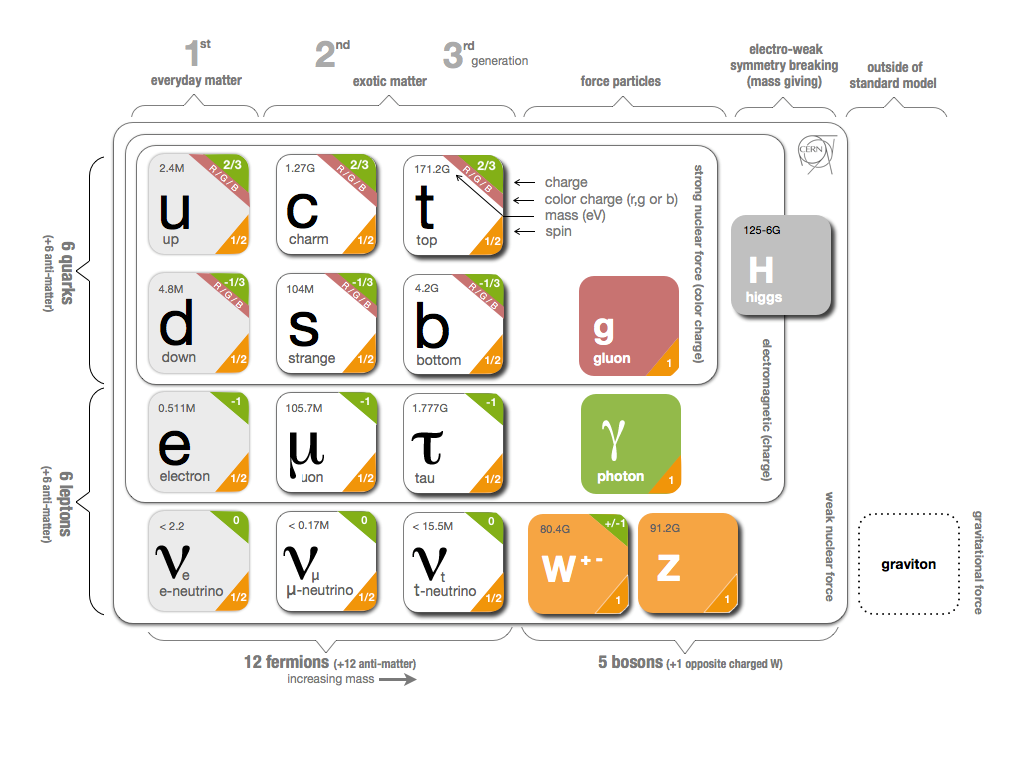
\includegraphics[width=6in]{images/SMinfographic_image}
    \caption[Standard Model Infographic]{An infographic of the Standard Model \cite{Purcell:1473657}. The elementary particles are arranged in their usual generational pairs and the surrounding solid lines divide them into sections based on the fundamental forces they experience.}
    \label{fig:SM}
\end{figure}

\subsection{Fermions}

The fermions encompass all forms of ordinary and exotic matter and obey Fermi-Dirac statistics because of their half-integer spin, namely, spin-\ensuremath{\frac{1}{2}}. They are divided into \textit{leptons} and \textit{quarks}. The electrically charged leptons interact via the electromagnetic and weak nuclear forces and include the familiar \textit{electron} (\lepe), the \textit{muon} (\lepm), and the \textit{tau} (\lept). The charged leptons also have neutral counterparts (\lepne, \lepnm, \lepnt) known as \textit{neutrinos}, which interact solely via the weak nuclear force. The quarks, having both electric and color charge, interact via the electromagnetic and strong and weak nuclear forces and include the up (\qrku), down (\qrkd), charm (\qrkc), strange (\qrks), bottom (\qrkb), and top (\qrkt). Although the leptons can exist freely, the nature of the strong interaction gives rise to color confinement, whereby quarks only appear within composite particles called hadrons. The bound states of quark doublets are known as mesons while those of quark triplets, of which the familiar proton is an example, are known as baryons.

The leptons and quarks are each arranged into pairs by flavour quantum number and sorted into three generations of increasing mass\footnote{The observation of neutrino oscillations disproved the prediction that they are massless but its implications for the lepton generations are unclear.}, as depicted in Figure \ref{fig:SM}. The more massive particles of the higher generations decay into the stable particles of the first generation, which corroborates the observation that ordinary matter consists of electrons and up and down quarks which are bound in protons and neutrons. There are no known constraints on the number of fermion generations, although experimental results suggest there are only three.

\subsection{Bosons}

The bosons, which obey Bose-Einstein statistics because of their integer spin, are divided into vector and scalar bosons. The spin-1 vector, or gauge, bosons mediate the fundamental forces and are exchanged between elementary particles during their interactions. The photon (\bosg) mediates the electromagnetic force, which is responsible for the phenomenon of intermolecular repulsion.\footnote{It is this repulsion that prevents us from passing through objects.} The \bosW\ and \bosZ\ bosons mediate the weak nuclear force that causes nuclear decay. And finally, the gluons (\bosgln) mediate the strong nuclear force that binds quarks into hadrons and even protons and neutrons in nuclei. The only spin-0 scalar boson in the theory is the Higgs boson (\bosH), which is responsible for the masses of the heavy gauge bosons and fermions.

\subsection{The Higgs Mechanism}

The requirement of gauge invariance under \symWEAK\ leads to a prediction of massless gauge bosons, which stands in contrast to the observation that the weak vector bosons are massive. In order to reconcile this observation while preserving the gauge invariance of the interaction, a mechanism of \textit{spontaneous symmetry breaking} was incorporated into the unified electroweak theory proposed by Sheldon Glashow \cite{EWKGLASHOW}, Abdus Salam \cite{EWKSALAM}, and Steven Weinberg \cite{EWKWEINBERG}. This mechanism, which came to be known as the \textit{Higgs mechanism}, was independently developed by Robert Brout and Fran\c{c}ois Englert \cite{HIGGSBE}, its namesake Peter Higgs \cite{HIGGSH}, and Gerald Guralnik, Richard Hagen, and Sir Thomas Kibble \cite{HIGGSGHK}.

The mechanism introduces into the Standard Model a scalar field $\phi$ represented as a complex doublet
\begin{equation}
  \phi = \begin{pmatrix}
           \phi^{+} \\
           \phi^{0} \\
         \end{pmatrix}
       = \frac{1}{\sqrt{2}}
         \begin{pmatrix}
           \phi_{1} + i\phi_{2} \\
           \phi_{3} + i\phi_{4} \\
         \end{pmatrix}
\end{equation}
and its potential $V(\phi)$ of the form
\begin{equation}
V(\phi) = \mu^{2}\phi^{\dag}\phi + \frac{\lambda}{2}(\phi^{\dag}\phi)^{2},
\end{equation}
where the real parameters $\mu^{2}$ and $\lambda$ represent the mass and self-coupling, respectively. The self-coupling $\lambda$ is taken to be positive by convention such that the potential is bounded from below. When $\mu^{2} > 0$, the potential is parabolic in shape and the ground state of the vacuum is at $\phi = 0$, keeping its symmetries intact. However, when $\mu^{2} < 0$, the minimum of the potential is no longer at $\phi = 0$ but rather\footnote{The solution is unique up to a phase $e^{i\theta}$, but it is customary to take $\theta = 0$.}
\begin{equation}
  v = \left(\frac{-\mu^{2}}{\lambda}\right)^{1/2},
  \label{eq:vev}
\end{equation}
where the vacuum now attains an expectation value $v$ in its ground state. The shape of such a potential is illustrated in Figure \ref{fig:potential}. The Higgs mechanism thus provides the means to spontaneously break the $\symWEAK \times \symEM$ symmetry within the model.

\begin{figure}[htbp]
  \centering
    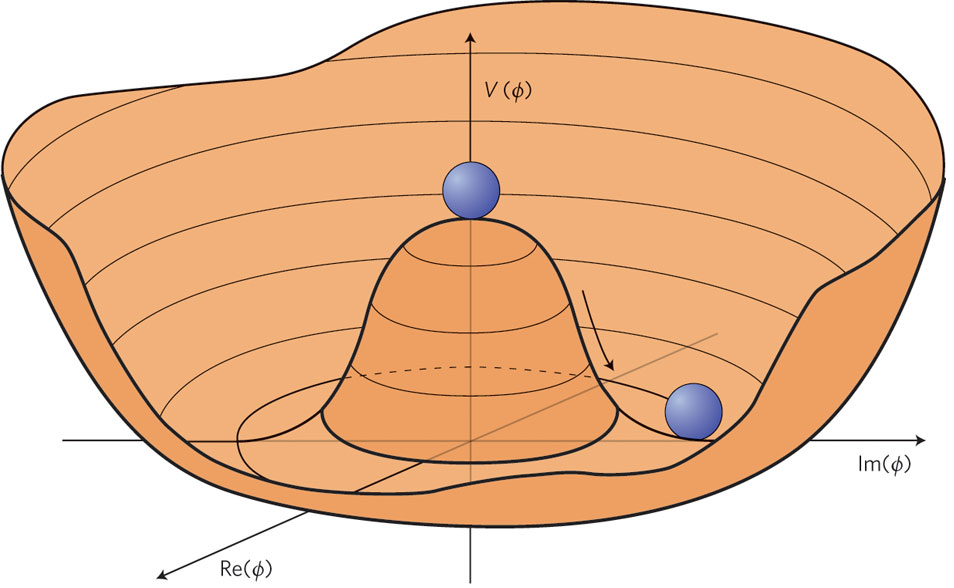
\includegraphics[width=3.5in]{images/higgspotential}
    \caption[Shape of the Higgs Field Potential]{The shape of the Higgs field potential for $\mu^{2} < 0$ \cite{deBoer:2013pud}. The transition of the field from its unstable state at the origin to its true ground state spontaneously breaks the rotational symmetry of the system.}
    \label{fig:potential}
\end{figure}

Because particles are excitations of their fields, the presence of the Higgs field also suggests the existence of the Higgs boson. An expression for the mass of this new boson can be determined by expanding the potential around the vacuum ground state $\phi_{0}$. By choosing the unitary gauge, the components of $\phi_{0}$ become
\begin{equation}
  (\phi_{1})_{0} = 0, (\phi_{2})_{0} = 0, (\phi_{3})_{0} = v, (\phi_{4})_{0} = 0
\end{equation}
and $\phi_{0}$ becomes simply
\begin{equation}
  \phi_{0} = \begin{pmatrix}
               \phi^{+} \\
               \phi^{0} \\
             \end{pmatrix}_{0}
           = \frac{1}{\sqrt{2}}
             \begin{pmatrix}
               0 \\
               v \\
             \end{pmatrix}.
\end{equation}
Then for small fluctuations $\phi(x) = \phi_{0} + H(x)$, the potential to second order in $H$ becomes
\begin{align}
  \begin{split}
    V(\phi) &= \frac{\mu^{2}}{2}(v^{2} + 2vH + H^{2}) + \frac{\lambda}{4}(v^{2} + 2vH + H^{2})^{2} \\
            &= \frac{1}{2}(\mu^{2}v^{2} + \frac{\lambda}{2}v^{4}) + (\mu^{2}v + \lambda v^{3})H + \frac{1}{2}(\mu^{2} + 3\lambda v^{2})H^{2} + \mathcal{O}(H^{3}) \\
            &= V_{0} - \frac{1}{2}(2\mu^{2})H^{2} + \mathcal{O}(H^{3}), \\
  \end{split}
  \label{eq:higgsexpand}
\end{align}
where $V_{0}$ collects the constant terms and Equation \ref{eq:vev} has been used to vanish the first order term and simplify the second order term. The mass can be read from the coefficient of the second order term in $H$:
\begin{equation}
  m_{H}^{2} = -2\mu^{2} \implies m_{H} = \sqrt{2}\mu = \sqrt{2\lambda}v,
\end{equation}
where the sign of the mass was dropped because $\mu^2$ was chosen to be negative. Although the Standard Model predicts a massive Higgs boson, its dependence on the value of the unknown self-coupling parameter $\lambda$ and the vacuum expectation value $v$ means it must be determined experimentally.

\subsubsection{Gauge boson masses}

The necessity of the Higgs mechanism is realized by how it generates the masses of the gauge bosons. The Lagrangian for the Higgs may be written as
\begin{equation}
  \mathcal{L}_{\phi} = (D_{\mu}\phi)^{\dag}(D^{\mu}\phi) - V(\phi) = (D_{\mu}\phi)^{\dag}(D^{\mu}\phi) - \mu^{2}\phi^{\dag}\phi - \frac{\lambda}{2}(\phi^{\dag}\phi)^{2},
  \label{eq:Lhiggs}
\end{equation}
By definition, the Higgs field has weak hypercharge $Y = +1$ and weak isospin $T_{3} = -1/2$. The weak hypercharge $Y$ and weak isospin $T$ are the generators of the \symWEAK\ and \symEM\ symmetries, respectively, with the choice of their values made to satisfy the relation
\begin{equation}
  Q = T_{3} + \frac{1}{2}Y,
\end{equation}
where $Q$ is the electric charge.\footnote{Hence, the Higgs boson is a neutral particle.} These choices require the covariant derivative of the kinetic term to be of the form
\begin{equation}
  D_{\mu}\phi = (\partial_{\mu} - \frac{i}{2}g\boldsymbol\sigma\cdot\mathbf{W}_{\mu} - \frac{i}{2}g^{\prime}B_{\mu})\phi,
\end{equation}
where $\mathbf{W_{\mu}}$ and $B_{\mu}$ are, respectively, the \symWEAK\ and \symEM\ gauge bosons, $g$ and $g^{\prime}$ are the corresponding gauge couplings, and $\boldsymbol\sigma = \sigma^{a}, a = 1, 2, 3$ are the Pauli matrices.

The gauge boson masses are contained in the kinetic term of the Lagrangian and can be determined by evaluating its expression for the vacuum ground state. The covariant derivative becomes
\begin{align}
  \begin{split}
    D_{\mu}\phi &\rightarrow \left[ \partial_{\mu} - \frac{i}{2}g \begin{pmatrix} W_{\mu}^{3} & W_{\mu}^{1} - iW_{\mu}^{2} \\ W_{\mu}^{1} + iW_{\mu}^{2} & -W_{\mu}^{3} \\ \end{pmatrix} - \frac{i}{2}g^{\prime}B_{\mu} \right] \frac{1}{\sqrt{2}} \begin{pmatrix} 0 \\ v + H \\ \end{pmatrix} \\[1em]
                &= -\frac{i}{2} \begin{pmatrix} \frac{g}{\sqrt{2}}(W_{\mu}^{1}-iW_{\mu}^{2})(v + H) \\ i\sqrt{2}\partial_{\mu}H + \frac{1}{\sqrt{2}}(-gW_{\mu}^{3} + g^{\prime}B_{\mu})(v + H) \\ \end{pmatrix} \\
  \end{split}
\end{align}
and substituting this expression into Equation \ref{eq:Lhiggs} while ignoring the potential term for clarity yields
\begin{align}
  \begin{split}
    \mathcal{L}_{\phi} &= \frac{1}{4} \begin{vmatrix} \frac{g}{\sqrt{2}}(W_{\mu}^{1}-iW_{\mu}^{2})(v + H) \\ i\sqrt{2}\partial_{\mu}H + \frac{1}{\sqrt{2}}(-gW_{\mu}^{3} + g^{\prime}B_{\mu})(v + H) \\ \end{vmatrix}^{2} \\[1em]
                       &= \frac{1}{4} \left[ 2(\partial_{\mu}H)^{2} + \left( \frac{g^{2}}{2} \left( (W_{\mu}^{1})^{2} + (W_{\mu}^{2})^{2} \right) + \frac{1}{2} \left( g^{\prime}B_{\mu} - gW_{\mu}^{3} \right)^{2} \right) (v + H)^{2} \right] \\[1em]
                       &= \frac{1}{2}(\partial_{\mu}H)^{2} + \frac{g^{2}}{8}(W_{\mu}^{1})^{2}v^{2} + \frac{g^{2}}{8}(W_{\mu}^{2})^{2}v^{2} + \frac{1}{8}\left( g^{\prime}B_{\mu} - gW_{\mu}^{3} \right)^{2}v^{2} + \mathcal{O}(H), \\
    \label{eq:gaugemasses}
  \end{split}
\end{align}
where higher order terms in $H$ have been discarded. The result of Equation \ref{eq:gaugemasses} reveals that the broken symmetry of the Higgs field causes the $W_{\mu}^{1}$ and $W_{\mu}^{2}$ vector fields to both acquire a mass of
\begin{equation}
  m_{W}^{2} = \frac{g^{2}v^{2}}{4} \implies m_{W} = \frac{gv}{2}.
\end{equation}
The linear combination of vector fields $(g^{\prime}B_{\mu} - gW_{\mu}^{3})$ also acquires a mass that depends on the couplings $g$ and $g^{\prime}$, and is typically expressed as
\begin{equation}
  m_{Z}^{2} = \frac{(g^{2} + g^{\prime 2}) v^{2}}{4} \implies m_{Z} = \frac{\sqrt{g^{2} + g^{\prime 2}} v}{2}.
\end{equation}
The excitations of these massive vector fields are the weak gauge bosons \bosWp, \bosWm, and \bosZn\ which have been observed in nature and whose masses have been measured\cite{PDG2018} to be
\begin{equation}
  m_{\bosWp} = m_{\bosWm} = 80.379 \pm 0.012\ \GeV\ \mathrm{and}\ m_{\bosZn} = 91.1876 \pm 0.0021\ \GeV.
\end{equation}

The derivation would be complete but for a missing gauge boson. Recall our earlier transformation to the unitary gauge which fixed three of the four degrees of freedom of the Higgs field. According to Goldstone's Theorem\cite{Goldstone}, these degrees of freedom become the longitudinal polarizations of the now massive weak gauge bosons. The untouched degree of freedom thus corresponds to the massless photon \bosg. By taking the electromagnetic field $A_{\mu}$ to be proportional to the missing linear combination of fields $(g^{\prime}W_{\mu}^{3} + gB_{\mu})$, it can be explicitly introduced into the kinetic term of the Lagrangian while remaining orthogonal to the other fields.

\subsubsection{Fermion masses}

Although the Dirac Lagrangian describes the dynamics of the fermions, it is inadequate for explaining their observed masses. This is because a Dirac mass term of the form
\begin{equation}
  m\bar{\psi}\psi = m(\bar{\psi}_{L} + \bar{\psi}_{R})(\psi_{L} + \psi_{R}) = m(\bar{\psi}_{L}\psi_{R} + \bar{\psi}_{R}\psi_{L})
\end{equation}
violates the gauge invariance of the model by coupling together left-handed and right-handed fermions which transform differently under both \symWEAK\ and \symEM. The masses of the fermions are instead another consequence of spontaneous symmetry breaking, and their coupling to the scalar Higgs field through Yukawa interactions gives rise to their mass terms in the Standard Model Lagrangian.

The Yukawa interaction of the first generation leptons to the Higgs field $\phi$ is given by
\begin{equation}
  \mathcal{L}_{\mathrm{Yukawa}} = -\lambda_{\lepe} \left( \bar{L} \phi \lepe_{R} + \lepebar_{R} \phi^{\dag} L\right),
\end{equation}
where $\lambda_{\lepe}$ is the coupling constant, the \symWEAK\ singlet $\lepe_{R}$ represents the right-handed electron, and the \symWEAK\ doublet $L$ represents the left-handed neutrino\footnote{The neutrinos have been experimentally measured, within uncertainties, to have left-handed helicity only.} and electron, i.e.
\begin{equation}
  L = \begin{pmatrix} \nu_{L} \\ \lepe_{L} \\ \end{pmatrix}.
\end{equation}
Evaluating this expression for the vacuum ground state yields the electron mass term
\begin{align}
  \begin{split}
    \mathcal{L}_{\mathrm{Yukawa}} &= -\lambda_{\lepe} \left( \bar{L} \phi_{0} \lepe_{R} + \lepebar_{R} \phi_{0}^{\dag} L\right) \\[1em]
                                  &= -\frac{\lambda_{\lepe}}{\sqrt{2}} \left[ \begin{pmatrix} \bar{\nu}_{L} & \lepebar_{L} \\ \end{pmatrix} \begin{pmatrix} 0 \\ v \\ \end{pmatrix}_{0} \lepe_{R} + \lepebar_{R} \begin{pmatrix} 0 & v \\ \end{pmatrix}_{0} \begin{pmatrix} \nu_{L} \\ \lepe_{L} \\ \end{pmatrix} \right] \\[1em]
                                  &= -\frac{\lambda_{\lepe}v}{\sqrt{2}} \left( \lepebar_{L} \lepe_{R} + \lepebar_{R} \lepe_{L} \right), \\[1em]
  \end{split}
\end{align}
which gives the electron mass
\begin{equation}
  m_{\lepe} = \frac{\lambda_{\lepe}v}{\sqrt{2}}.
\end{equation}
Therefore the electron, and similarly for the charged leptons of the other generations, is a mixture of left-handed and right-handed fields which acquire a mass that is proportional to the vacuum expectation value $v$ and their coupling to the Higgs field.

The Yukawa interaction of the quarks, taking into account the existence of the right-handed \symWEAK\ singlet $\qrku_{R}$, is similarly given by
\begin{equation}
  \mathcal{L}_{\mathrm{Yukawa}} = -\Lambda_{\qrkd}^{ij} \left( \bar{Q}_{L}^{i} \phi \qrkd_{R}^{j} + \qrkdbar_{R}^{j} \phi^{\dag} Q_{L}^{i} \right) -\Lambda_{\qrku}^{ij} \left( \bar{Q}_{L}^{i} \tilde{\phi} \qrku_{R}^{j} + \qrkubar_{R}^{j} \tilde{\phi}^{\dag} Q_{L}^{i} \right),
\end{equation}
where $\Lambda_{\qrkd}^{ij}$ and $\Lambda_{\qrku}^{ij}$ are $3 \times 3$ complex matrices of couplings for the down-type and up-type quarks, respectively, whose indices $i$ and $j$ run over the quark generations, $\qrkd_{R}$ and $\qrku_{R}$ are the right-handed singlets, $Q_{L}$ is the left-handed doublet
\begin{equation}
  Q_{L} = \begin{pmatrix} u_{L} \\ d_{L} \\ \end{pmatrix},
\end{equation}
and $\tilde{\phi}$ is the charge conjugate of the Higgs doublet
\begin{equation}
  \tilde{\phi} = \begin{pmatrix} \phi^{0*} \\ -\phi^{+*} \\ \end{pmatrix} \implies \tilde{\phi}_{0} = \begin{pmatrix} v \\ 0 \\ \end{pmatrix}.
\end{equation}
Proceeding as before, evaluating this expression for the vacuum ground state yields
\begin{equation}
  \mathcal{L}_{\mathrm{Yukawa}} = -\frac{v}{\sqrt{2}} \Lambda_{\qrkd}^{ij} \left( \qrkdbar_{L}^{i} \qrkd_{R}^{j} + \qrkdbar_{R}^{j} \qrkd_{L}^{i} \right) -\frac{v}{\sqrt{2}} \Lambda_{\qrku}^{ij} \left( \qrkubar_{L}^{i}\qrku_{R}^{j} + \qrkubar_{R}^{j} \qrku_{L}^{i} \right),
\end{equation}
from which the quark masses are found to be
\begin{equation}
  M_{\qrkd}^{ij} = \frac{\Lambda_{\qrkd}^{ij}v}{\sqrt{2}}\ \mathrm{and}\ M_{\qrku}^{ij} = \frac{\Lambda_{\qrku}^{ij}v}{\sqrt{2}}.
\end{equation}
These mass terms resemble those of leptons except that they are matrices which depend on the Yukawa couplings of the mixed quark states to the Higgs field. The physical quark fields correspond to the mass eigenstates obtained by diagonalizing the mass matrices $M_{\qrkd}^{ij}$ and $M_{\qrku}^{ij}$. A general complex matrix may be diagonalized by a biunitary transformation, so there exist unitary matrices $\mathbf{D}_{L}$, $\mathbf{D}_{R}$, $\mathbf{U}_{L}$, and $\mathbf{U}_{R}$ such that
\begin{equation}
  \mathbf{D}_{L}^{\dag}\mathbf{M}_{\qrkd}\mathbf{D}_{R} = \begin{pmatrix} m_{\qrkd} & 0 & 0 \\ 0 & m_{\qrks} & 0 \\ 0 & 0 & m_{\qrkb} \\ \end{pmatrix},\ \mathbf{U}_{L}^{\dag}\mathbf{M}_{\qrku}\mathbf{U}_{R} = \begin{pmatrix} m_{\qrku} & 0 & 0 \\ 0 & m_{\qrkc} & 0 \\ 0 & 0 & m_{\qrkt} \\ \end{pmatrix},
\end{equation}
where the mass eigenvalues are real and positive. But this transformation also amounts to diagonalizing the Yukawa coupling matrices, thus revealing that the quark masses also depend on their couplings and the vacuum expectation value in the same fashion as the charged leptons.

\section{The Higgs Boson}

While the Standard Model predicts the existence of the Higgs boson, it does not predict the value of its self-coupling $\lambda$ and therefore its mass \massH\ is an unknown parameter of the model. Theoretical constraints based on unitarity bounds, the stability of the vacuum, and the energy scale of Standard Model physics only place the value of \massH\ within a wide range from 100 \GeV\ up to 1 \TeV. Stronger limits on \massH, not to mention an observation of the elusive boson, would have to be obtained from experimental results. During the 1980s, experimental searches for the Higgs boson began in earnest as particle accelerators finally reached energies that enabled the predicted mass range to be studied. The current era of high-energy physics experiment is now dominated by experiments at the Large Hadron Collider (LHC) and so the following qualitative review of Standard Model Higgs boson phenomenology is framed in its context.

\subsection{Phenomenology}

The Standard Model Higgs boson is predicted to be a spinless particle with zero electric or color charge that is even under the combined symmetry of charge conjugation and parity (CP-symmetry). It is also predicted to couple to the gauge bosons, fermions, and itself\footnote{The Higgs self-couplings come from the higher order terms of Equation \ref{eq:higgsexpand}.} in proportion to their masses according to
\begin{equation}
  \begin{array}{ccc}
    g_{Hf\bar{f}} = \frac{m_{f}}{v}, & g_{HVV} = \frac{2m_{V}^{2}}{v}, & g_{HHVV} = \frac{2m_{V}^{2}}{v^{2}}, \\[1em]
    g_{HHH} = \frac{3m_{H}^{2}}{v},  & g_{HHHH} = \frac{3m_{H}^{2}}{v^{2}}, \\
  \end{array}
\end{equation}
where $V = \bosW\ \mathrm{or}\ \bosZ$ and $v$ is the vacuum expectation value.\cite{PDG2018} These interactions may be expressed as the Feynman diagram vertices shown in Figure \ref{fig:higgsvertices}. Because the Higgs boson might be coaxed into existence by these interactions, the production modes of the Higgs boson have informed the development of modern hadron colliders. By the same token, those interactions provide the means for the massive Higgs boson to decay into lighter and more stable particles. The decay modes of the Higgs boson thus influence the design of particle detectors capable of accurately measuring the properties of its decays products.

\begin{figure}[htbp]
  \centering
  \mbox{
    \subfigure [] {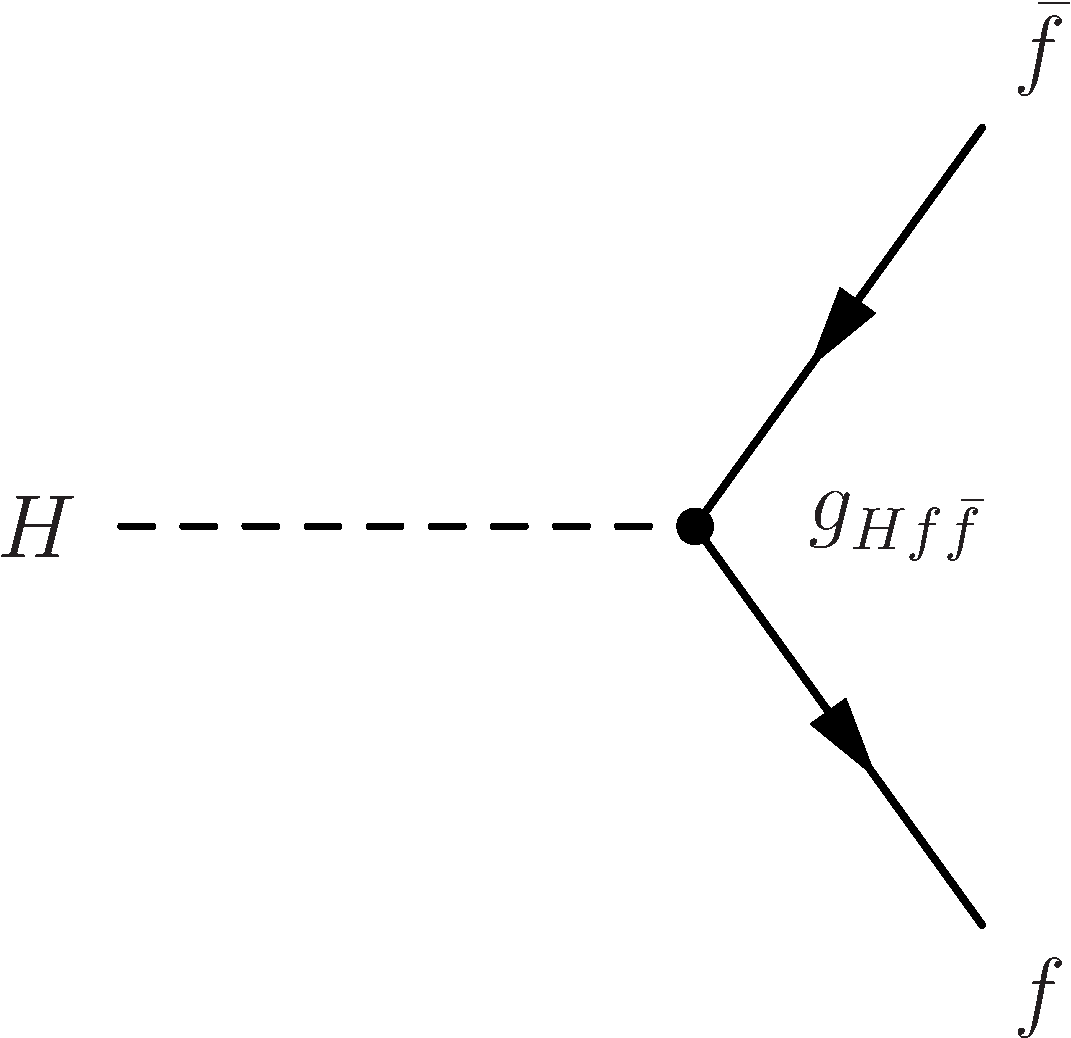
\includegraphics[scale=0.2]{images/vertex-Hff}} \qquad
    \subfigure [] {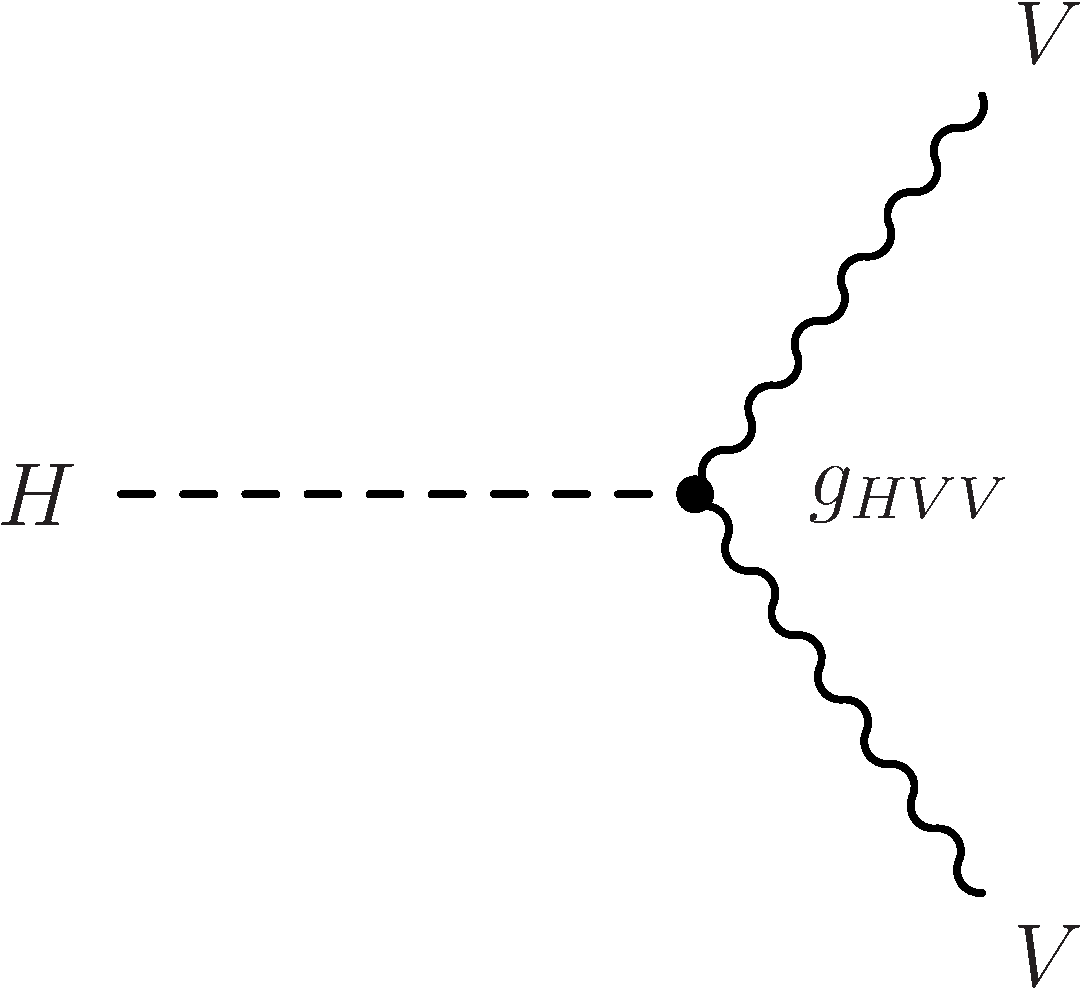
\includegraphics[scale=0.2]{images/vertex-HVV}} \qquad
    \subfigure [] {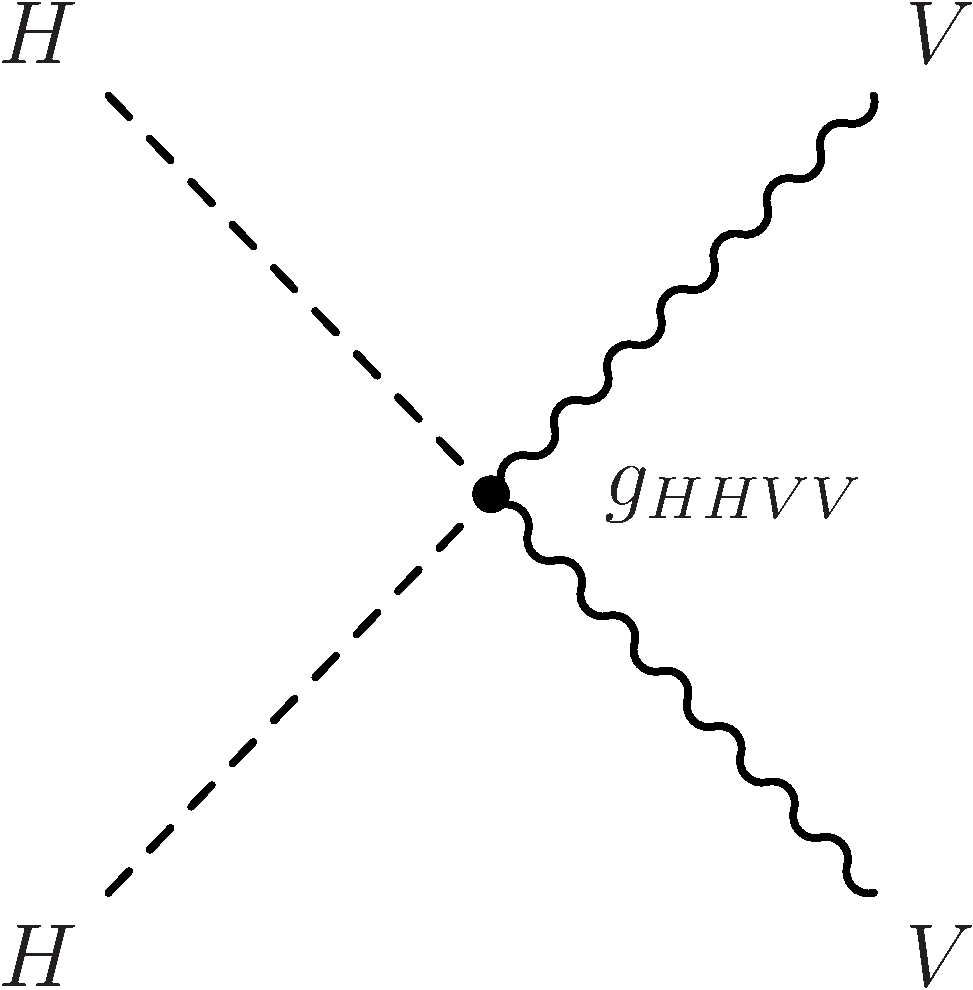
\includegraphics[scale=0.2]{images/vertex-HHVV}} \qquad
  }
  \mbox{
    \subfigure [] {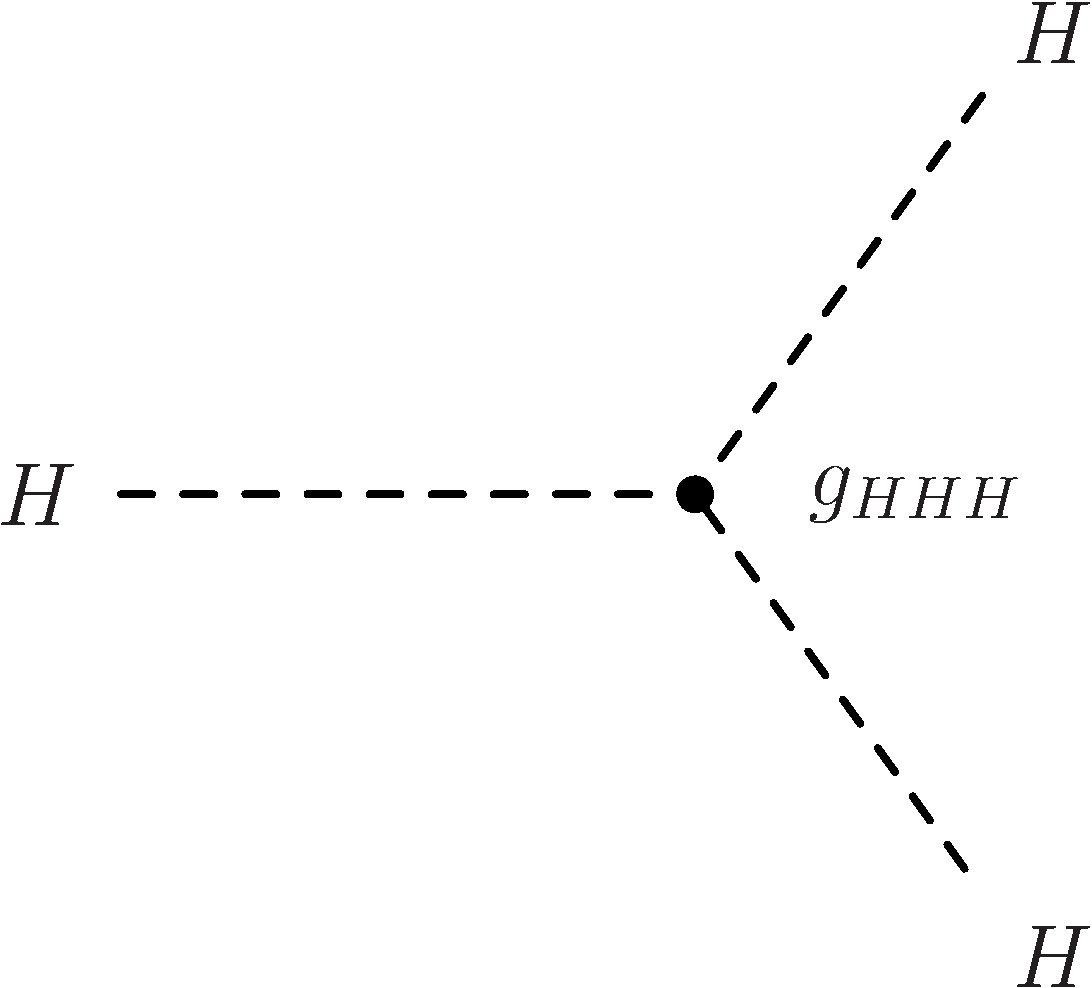
\includegraphics[scale=0.2]{images/vertex-HHH}} \qquad
    \subfigure [] {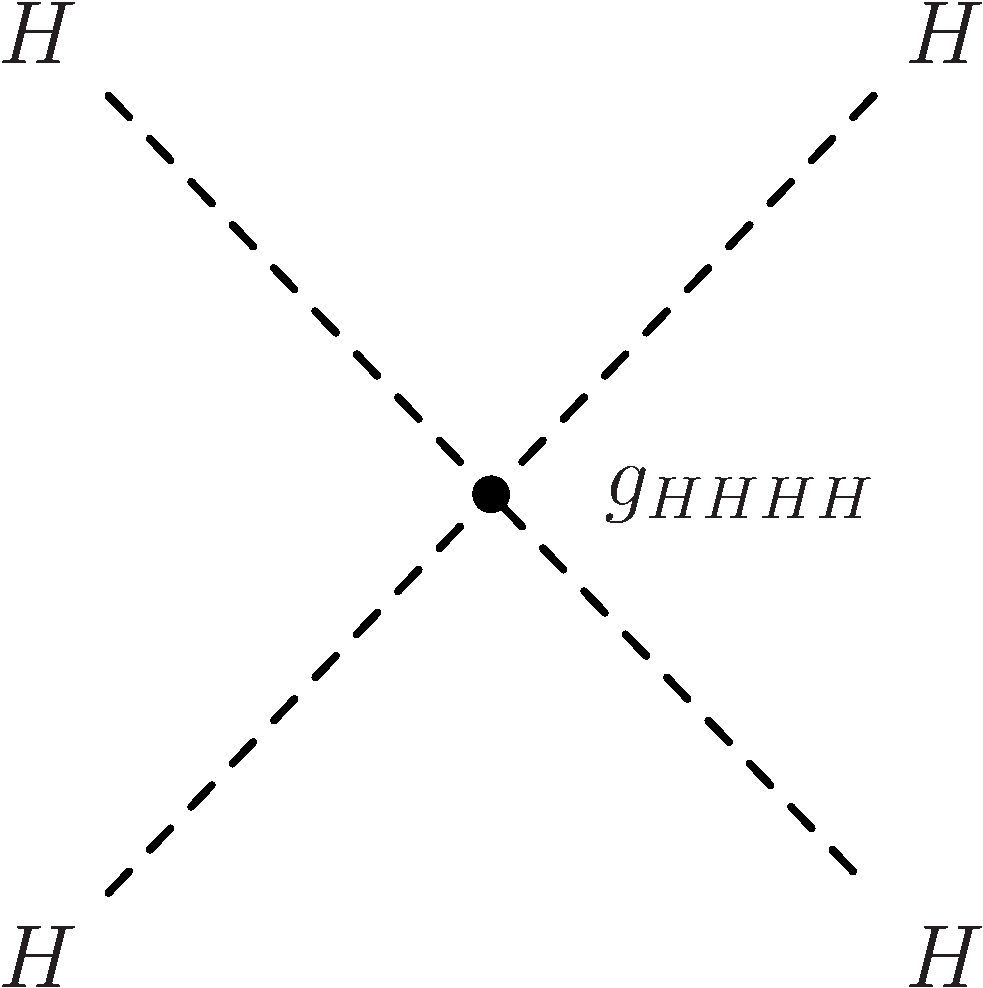
\includegraphics[scale=0.2]{images/vertex-HHHH}} \qquad
  }
  \caption[Higgs Boson Interaction Vertices]{The Feynman diagrams for the vertices of the Standard Model Higgs boson representing the A) fermion-Higgs interaction; B) trilinear gauge-Higgs interaction; C) quartic gauge-Higgs interaction; D) trilinear self-interaction; E) quartic self-interaction.}
  \label{fig:higgsvertices}
\end{figure}
 
\subsubsection{Production modes} \label{productionmodes}

The production of massive particles such as the Higgs boson proceeds from the interactions of hadrons made to collide at high energies. The probability that such a collision results in a specific interaction is known as a cross section $\sigma$. The production cross sections of the Higgs boson depend on the center-of-mass energy of the collision $\sqrt{s}$ and its mass \massH, and have been determined by theoretical calculations to behave as shown in Figure \ref{fig:higgsprodxsec}.

\begin{figure}[htbp]
  \centering
  \mbox{
    \subfigure [] {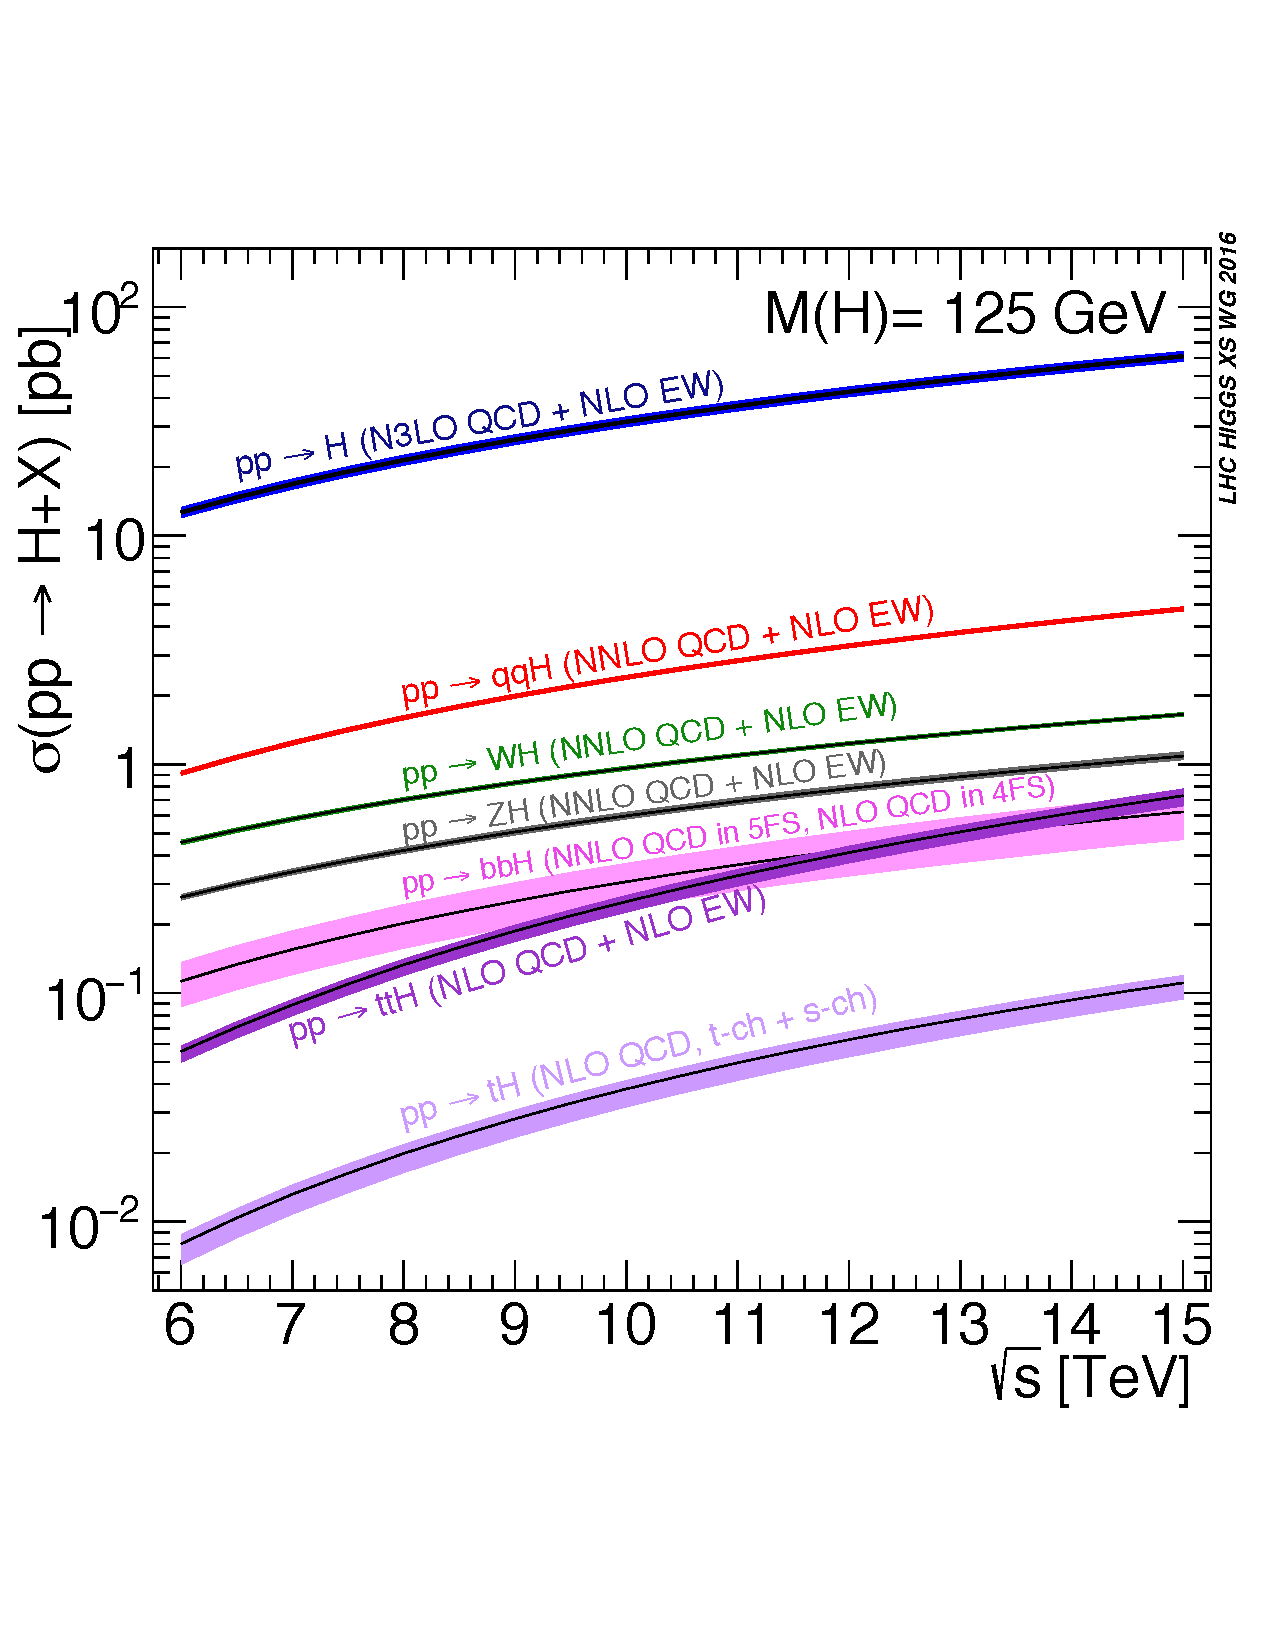
\includegraphics[scale=0.36]{images/Plot_Escan_H125_new_sqrt}} \qquad
    \subfigure [] {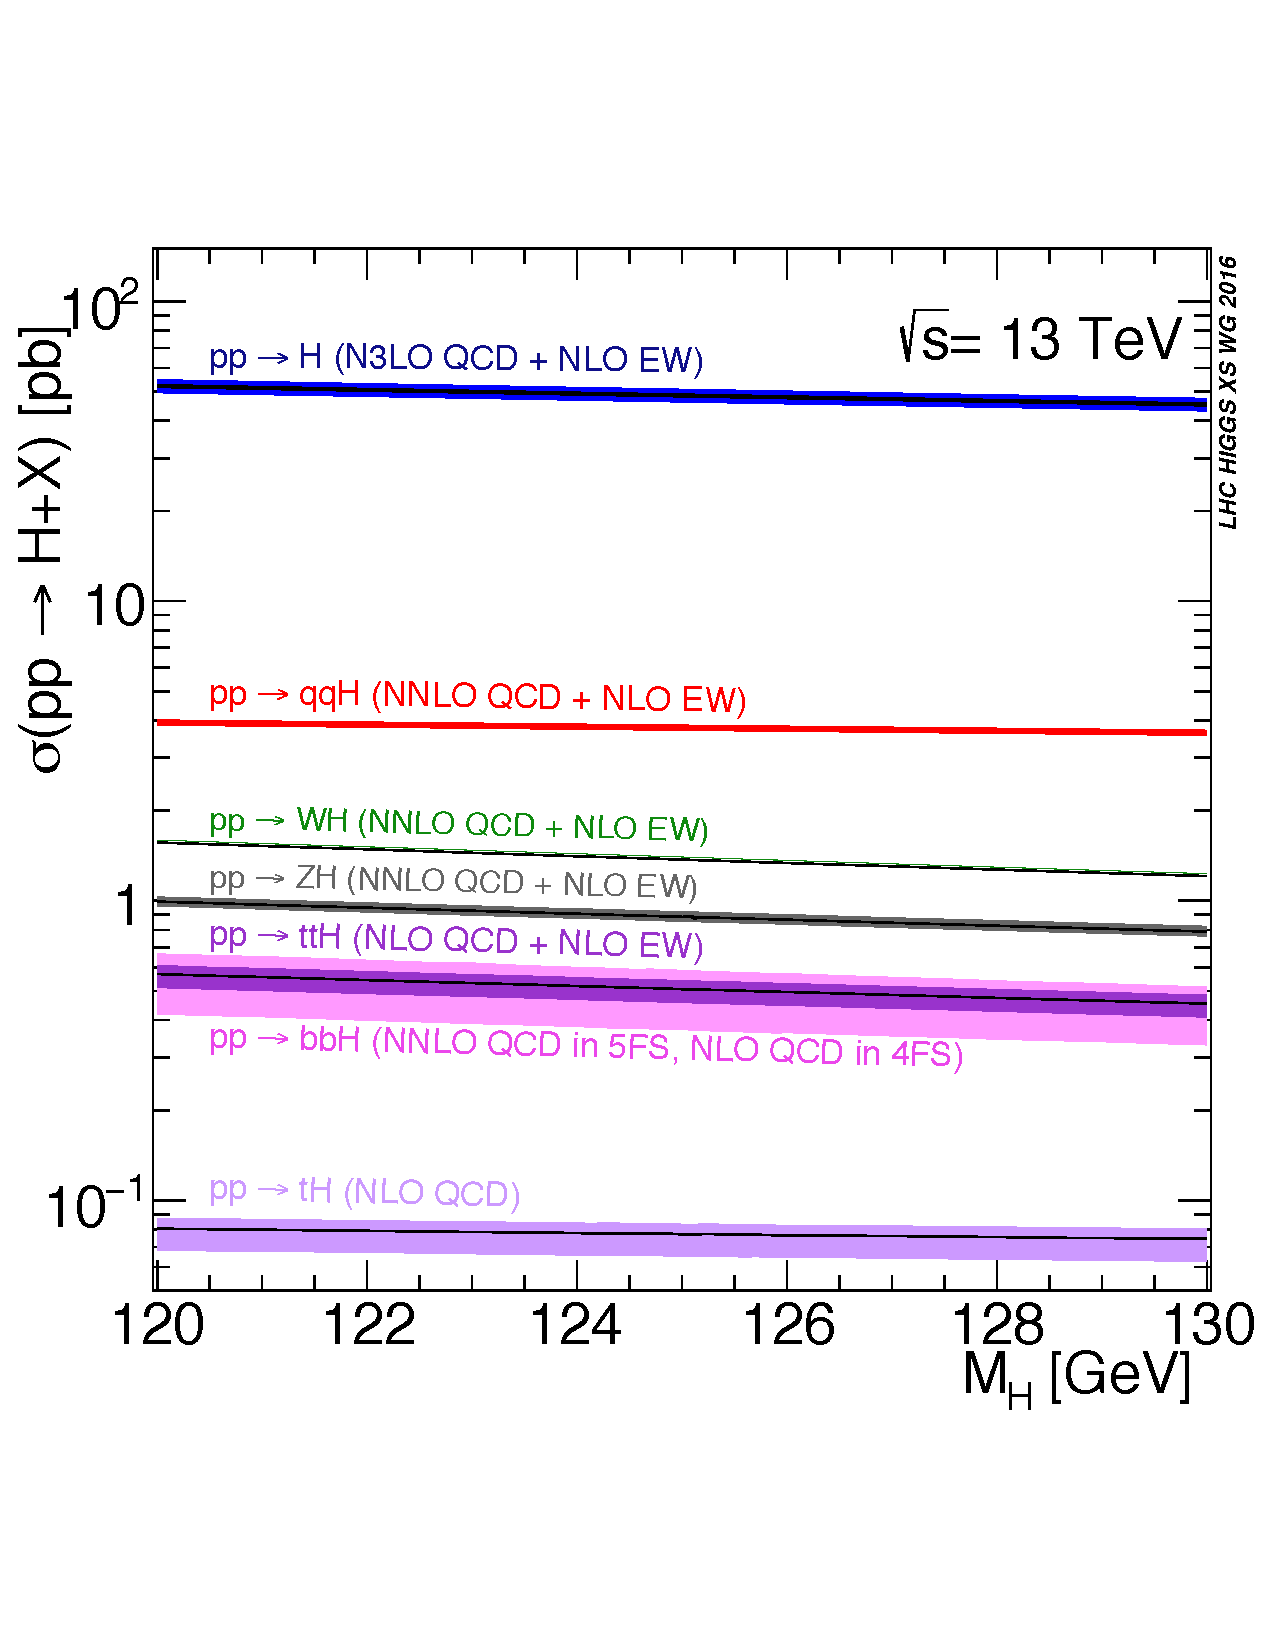
\includegraphics[scale=0.36]{images/plot_13tev_H_sqrt}} \qquad
  }
  \caption[Higgs Boson Production Cross Sections]{The production cross section for the Higgs boson as A) a function of the center of mass energy $\sqrt{s}$ for $\massH = 125\ \GeV$; B) a function of \massH\ for $\sqrt{s} = 13\ \TeV$. The shaded bands show the combined parametric and theoretical uncertainties and the labels indicate the production mode and any radiative corrections considered.\cite{CERNYR4}}
  \label{fig:higgsprodxsec}
\end{figure}

The dominant production mode is gluon fusion ($pp \rightarrow H$), in which a gluon from each of the colliding hadrons form a virtual quark loop. Because the Higgs boson couples to quarks in proportion to their masses, it can be radiated from the resulting virtual top quark or, to a lesser extent, bottom quark loop. The production mode with the second-largest cross section is vector boson fusion ($pp \rightarrow qqH$), which proceeds from the parton scattering of two quarks, or anti-quarks, via their exchange of weak vector bosons \bosV. This produces a Higgs boson because of the allowed trilinear gauge-Higgs interaction. The vector boson associated production mode ($pp \rightarrow \VH$), or \textit{Higgstrahlung}, has the third-largest cross section. This production mechanism proceeds from the weak interaction of a quark and an anti-quark from which a Higgs boson is radiated by the virtual \bosW\ or \bosZ\ weak vector boson. Because the \bosZ\ associated production can also be induced via a virtual top quark loop, contributions of nearly 15\% to the total production cross section of this mode come from the process $\bosgln\bosgln \rightarrow \bosZ\bosH$. The fourth relevant production mode is top quark pair associated production ($pp \rightarrow ttH$). Rather than forming a virtual top quark loop, a gluon from each of the colliding hadrons decays into a top quark-antiquark pair and a Higgs boson is produced by the annhiliation of a top quark of one pair and the top anti-quark of the other. The smallest cross sections are contributed by the single top quark associated production and bottom quark pair associated production modes, which are suppressed relative to the main production modes. The Feynman diagrams for the main production modes are shown in Figure \ref{fig:higgsprodfeyn}.

\begin{figure}[htbp]
  \centering
  \mbox{
    \subfigure [] {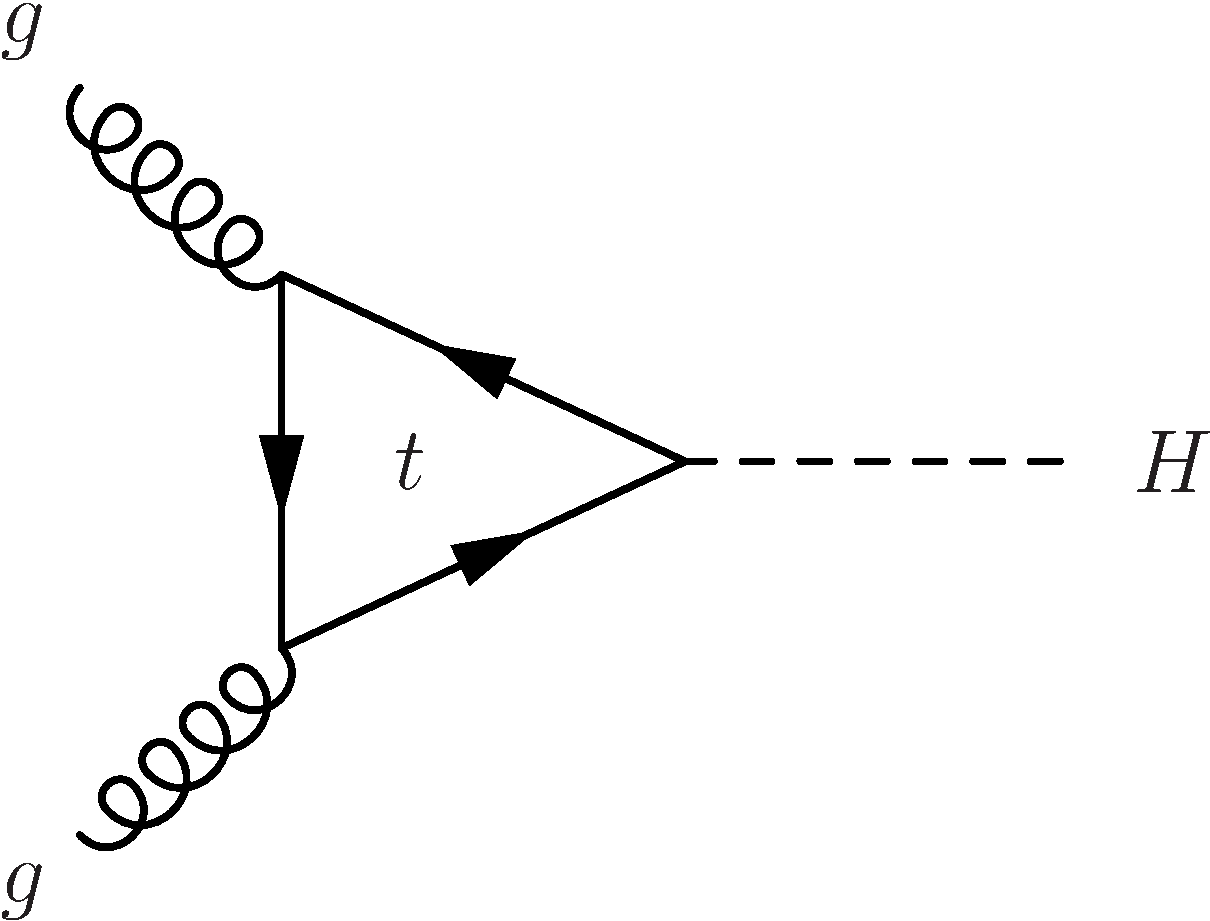
\includegraphics[scale=0.2]{images/production-ggH}} \qquad
    \subfigure [] {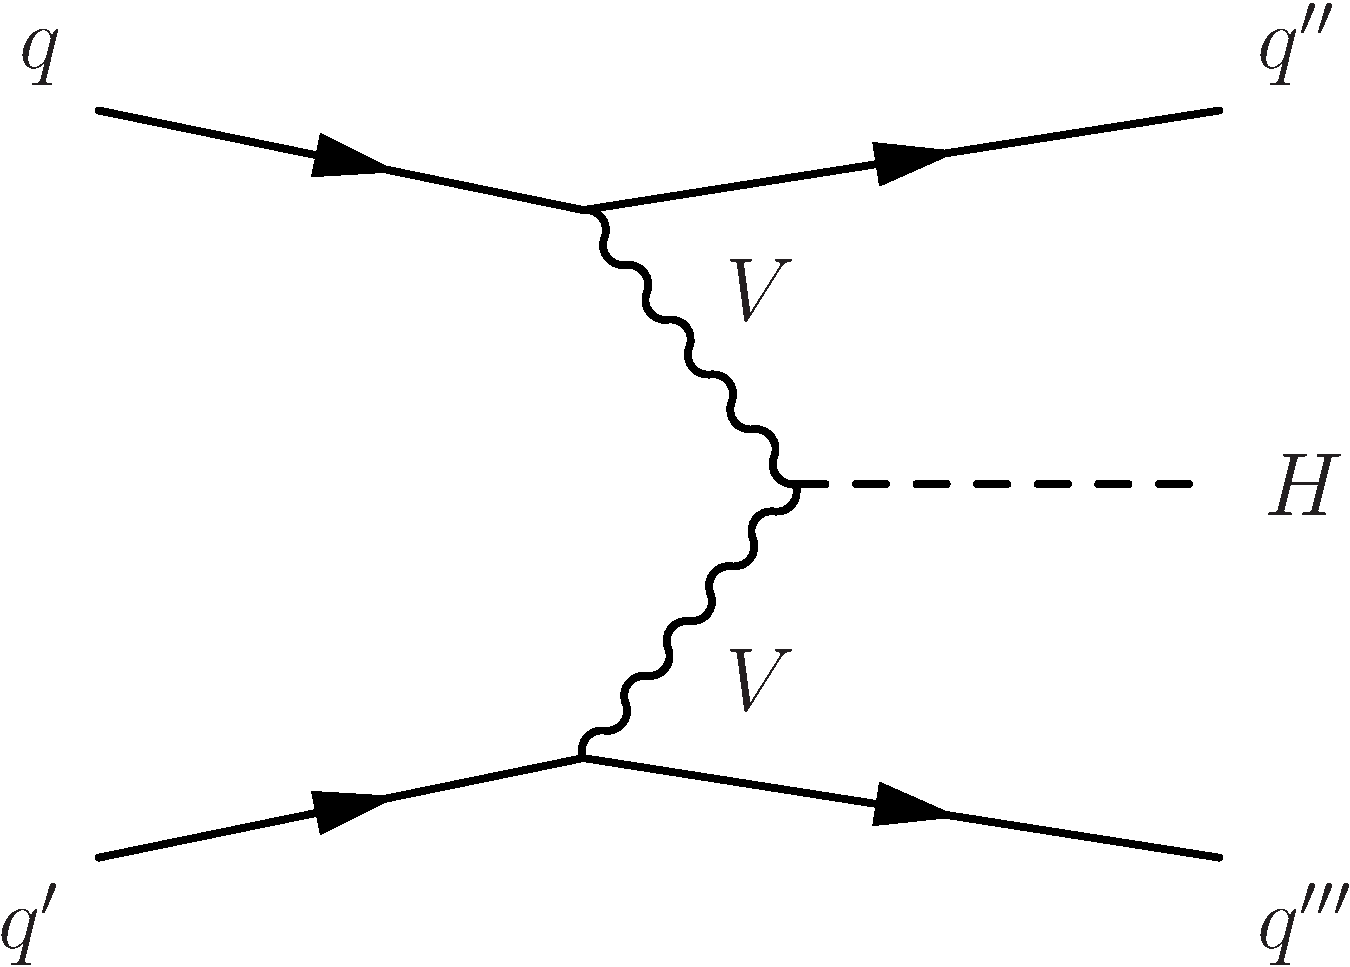
\includegraphics[scale=0.2]{images/production-VBF}} \qquad
    \subfigure [] {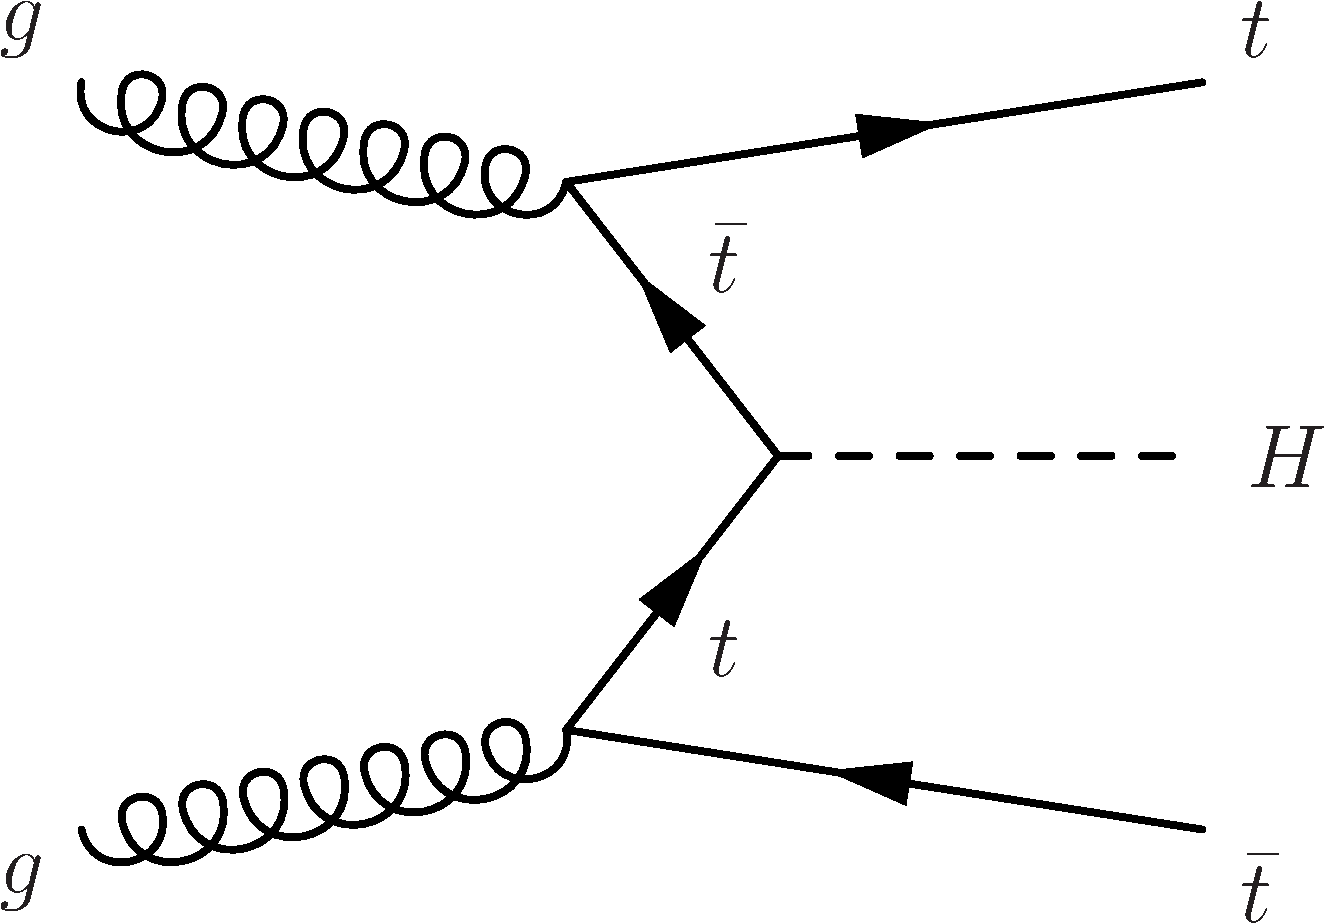
\includegraphics[scale=0.2]{images/production-ttH}} \qquad
  }
  \mbox{
    \subfigure [] {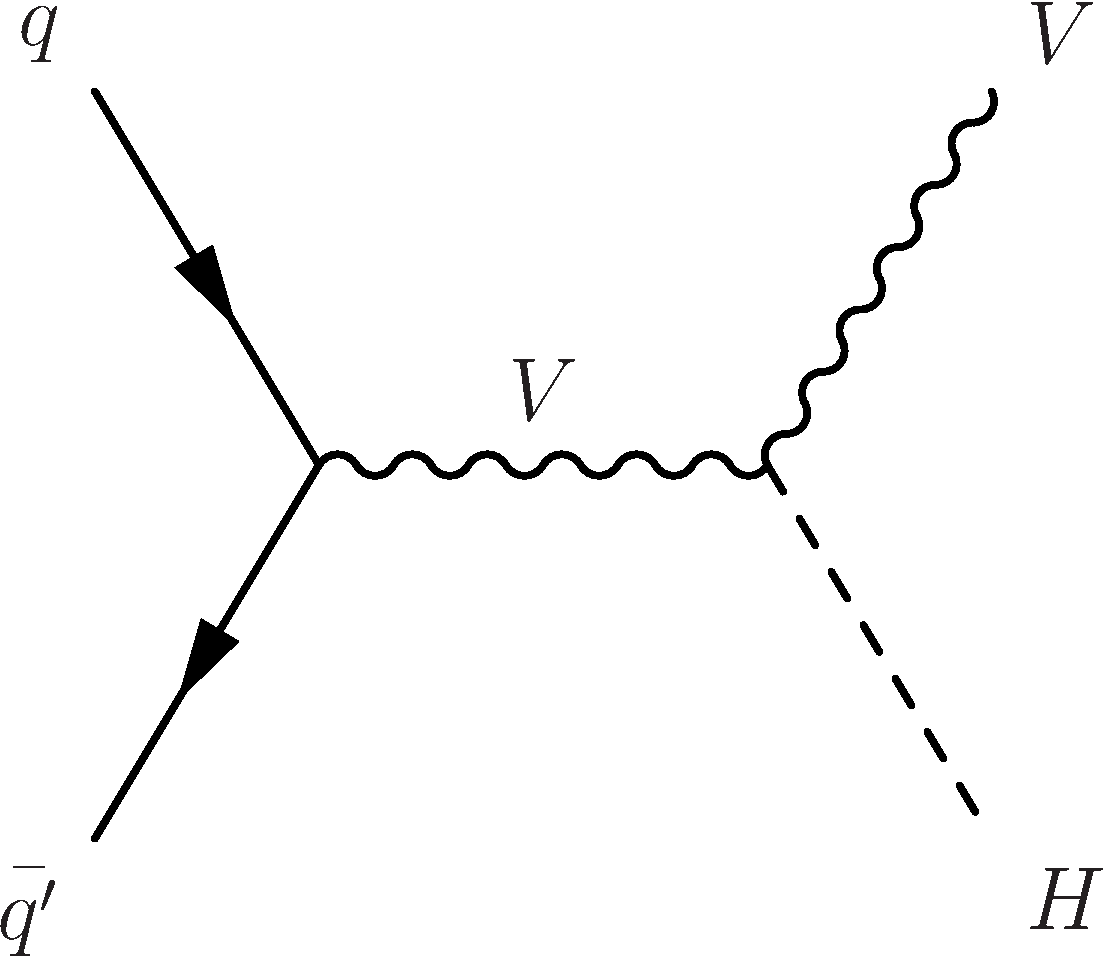
\includegraphics[scale=0.2]{images/production-VH}} \qquad
    \subfigure [] {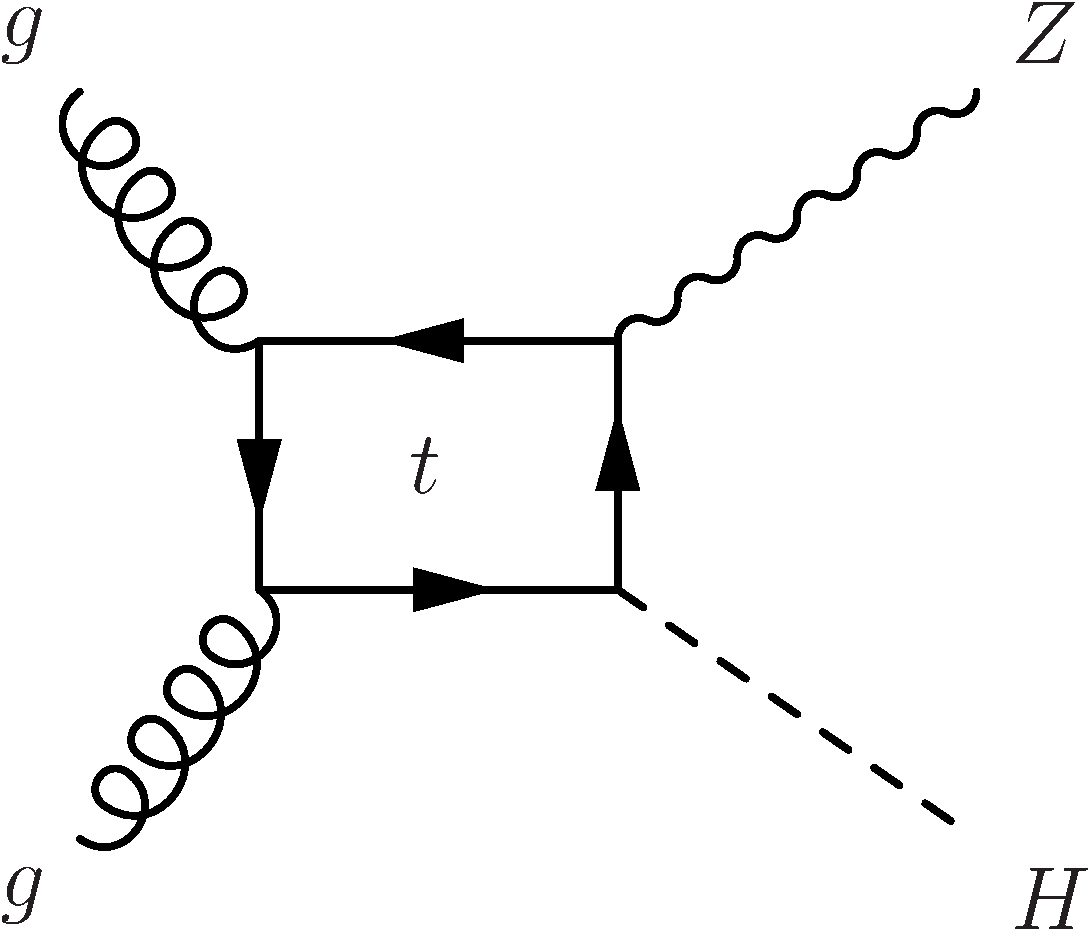
\includegraphics[scale=0.2]{images/production-ggZHbox_v2}} \qquad
    \subfigure [] {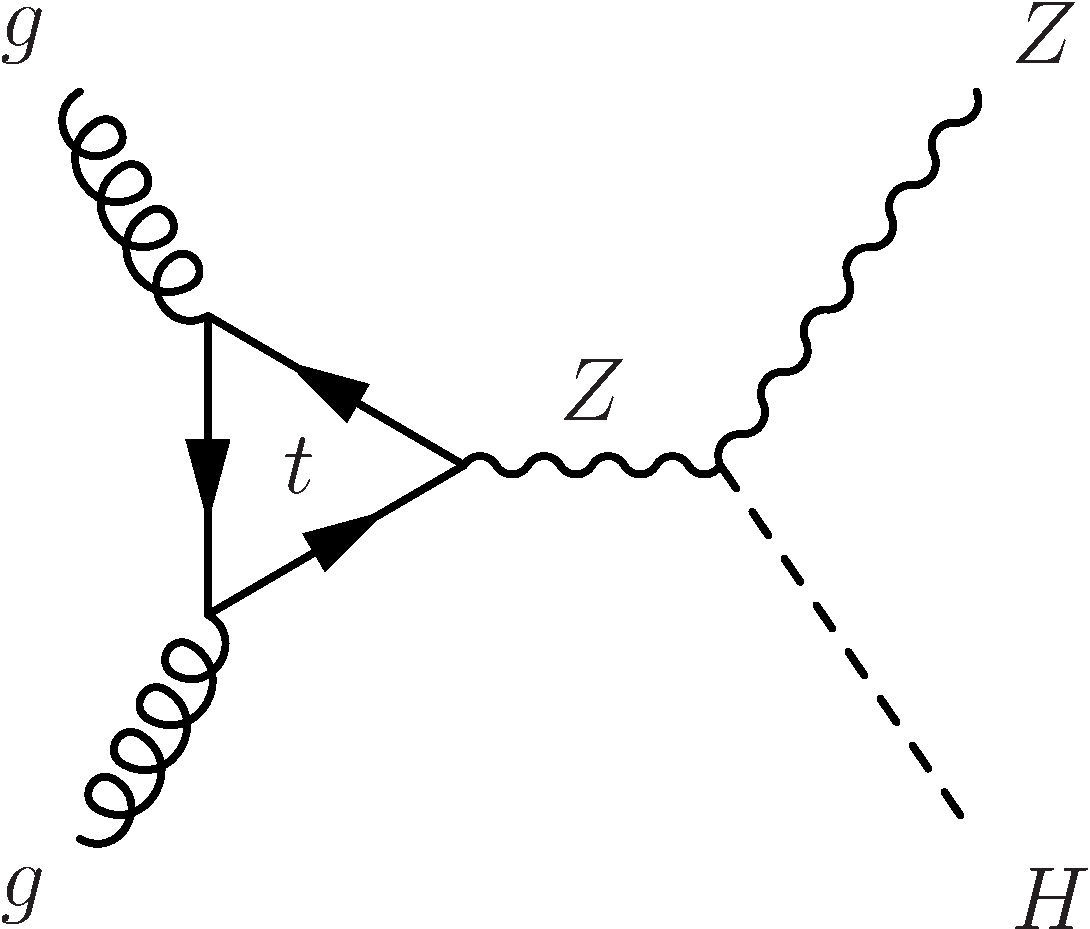
\includegraphics[scale=0.2]{images/production-ggZH}} \qquad
  }
  \caption[Higgs Boson Production Diagrams]{The Feynman diagrams for the Higgs boson production processes of A) gluon fusion; B) vector boson fusion; C) top quark pair associated production; D) vector boson associated production; E), D) top-loop induced contributions to the \bosZ\ boson associated production.}
  \label{fig:higgsprodfeyn}
\end{figure}

For the current center-of-mass energy of proton collisions at the LHC, $\sqrt{s} = 13\ \TeV$, and a Higgs boson mass of $\massH = 125\ \GeV$, the state-of-the-art values computed for the production cross sections\footnote{The cross sections are presented in units of picobarns $(\pb)$, where $1\ \mathrm{barn} = 10^{-24}\ \mathrm{cm}^{2}$.} are
\begin{alignat*}{2}
  &\sigma\left( pp \rightarrow H \right) &&= 48.58\ {}_{-6.7\%}^{+4.6\%} \ (\mathrm{theory}) \pm 3.2\%\ (\mathrm{PDF} + \alpha_{s})\ \pb, \\
  &\sigma\left( pp \rightarrow qqH \right) &&= 3.782\ {}_{-0.3\%}^{+0.4\%} \ (\mathrm{QCD\ scale}) \pm 2.1\%\ (\mathrm{PDF} + \alpha_{s})\ \pb, \\
  &\sigma\left( pp \rightarrow WH \right) &&= 1.373\ {}_{-0.7\%}^{+0.5\%} \ (\mathrm{QCD\ scale}) \pm 1.9\%\ (\mathrm{PDF} + \alpha_{s})\ \pb,
\end{alignat*}
\begin{alignat*}{2}
  &\sigma_{\mathrm{total}}\left( pp \rightarrow ZH \right) &&= 0.8839\ {}_{-3.1\%}^{+3.8\%} \ (\mathrm{QCD\ scale}) \pm 1.6\%\ (\mathrm{PDF} + \alpha_{s})\ \pb, \\
  &\sigma\left( gg \rightarrow ZH \right) &&= 0.1227\ {}_{-18.9\%}^{+25.1\%} \ (\mathrm{QCD\ scale}) \pm 2.4\%\ (\mathrm{PDF} + \alpha_{s})\ \pb, \\
  &\sigma\left( pp \rightarrow ttH \right) &&= 0.5071\ {}_{-9.2\%}^{+5.8\%} \ (\mathrm{QCD\ scale}) \pm 3.6\%\ (\mathrm{PDF} + \alpha_{s})\ \pb.
\end{alignat*}
The uncertainties are due to variations on the QCD renormalization scale ($\mathrm{QCD\ scale}$), the parton distribution function (PDF) that determines the momenta of the interacting partons, and the strong coupling constant ($\alpha_{s}$). The accuracy of these cross sections are determined by the inclusion of higher-order terms during their calculation, which is generally next-to-next-to-leading (NNLO) order in QCD and next-to-leading order (NLO) in electroweak corrections. The exceptions are that the gluon fusion cross section is calculated further to N3LO in QCD, hence acquiring additional theoretical uncertainties, and the top quark pair associated production cross section which is calculated only to NLO in QCD. The methods and theoretical treatment of these cross section calculations are thoroughly documented in Ref. \cite{CERNYR4}.

\subsubsection{Decay modes} \label{decaymodes}

With a predicted lifetime\footnote{The total decay width of the Higgs boson is predicted to be $\Gamma_{H} = 4.088$ \MeV\ and the lifetime of a particle is given by $\tau = \hslash\ /\ \Gamma$.} of $1.6 \times 10^{-22}\ \mathrm{s}$, the Higgs boson decays almost immediately and its presence can only be inferred from its decay products. Based on its predicted properties, the final state of its decay must be electrically and color neutral. By conservation of mass, it must also decay into lighter particles so, for example, a decay into a top quark-antiquark pair $t\bar{t}$ is forbidden for low mass Higgs bosons. However, because the Higgs boson couples to particles in proportion to their masses, the heaviest allowed decays will be the most favored.

\begin{figure}[htbp]
  \centering
    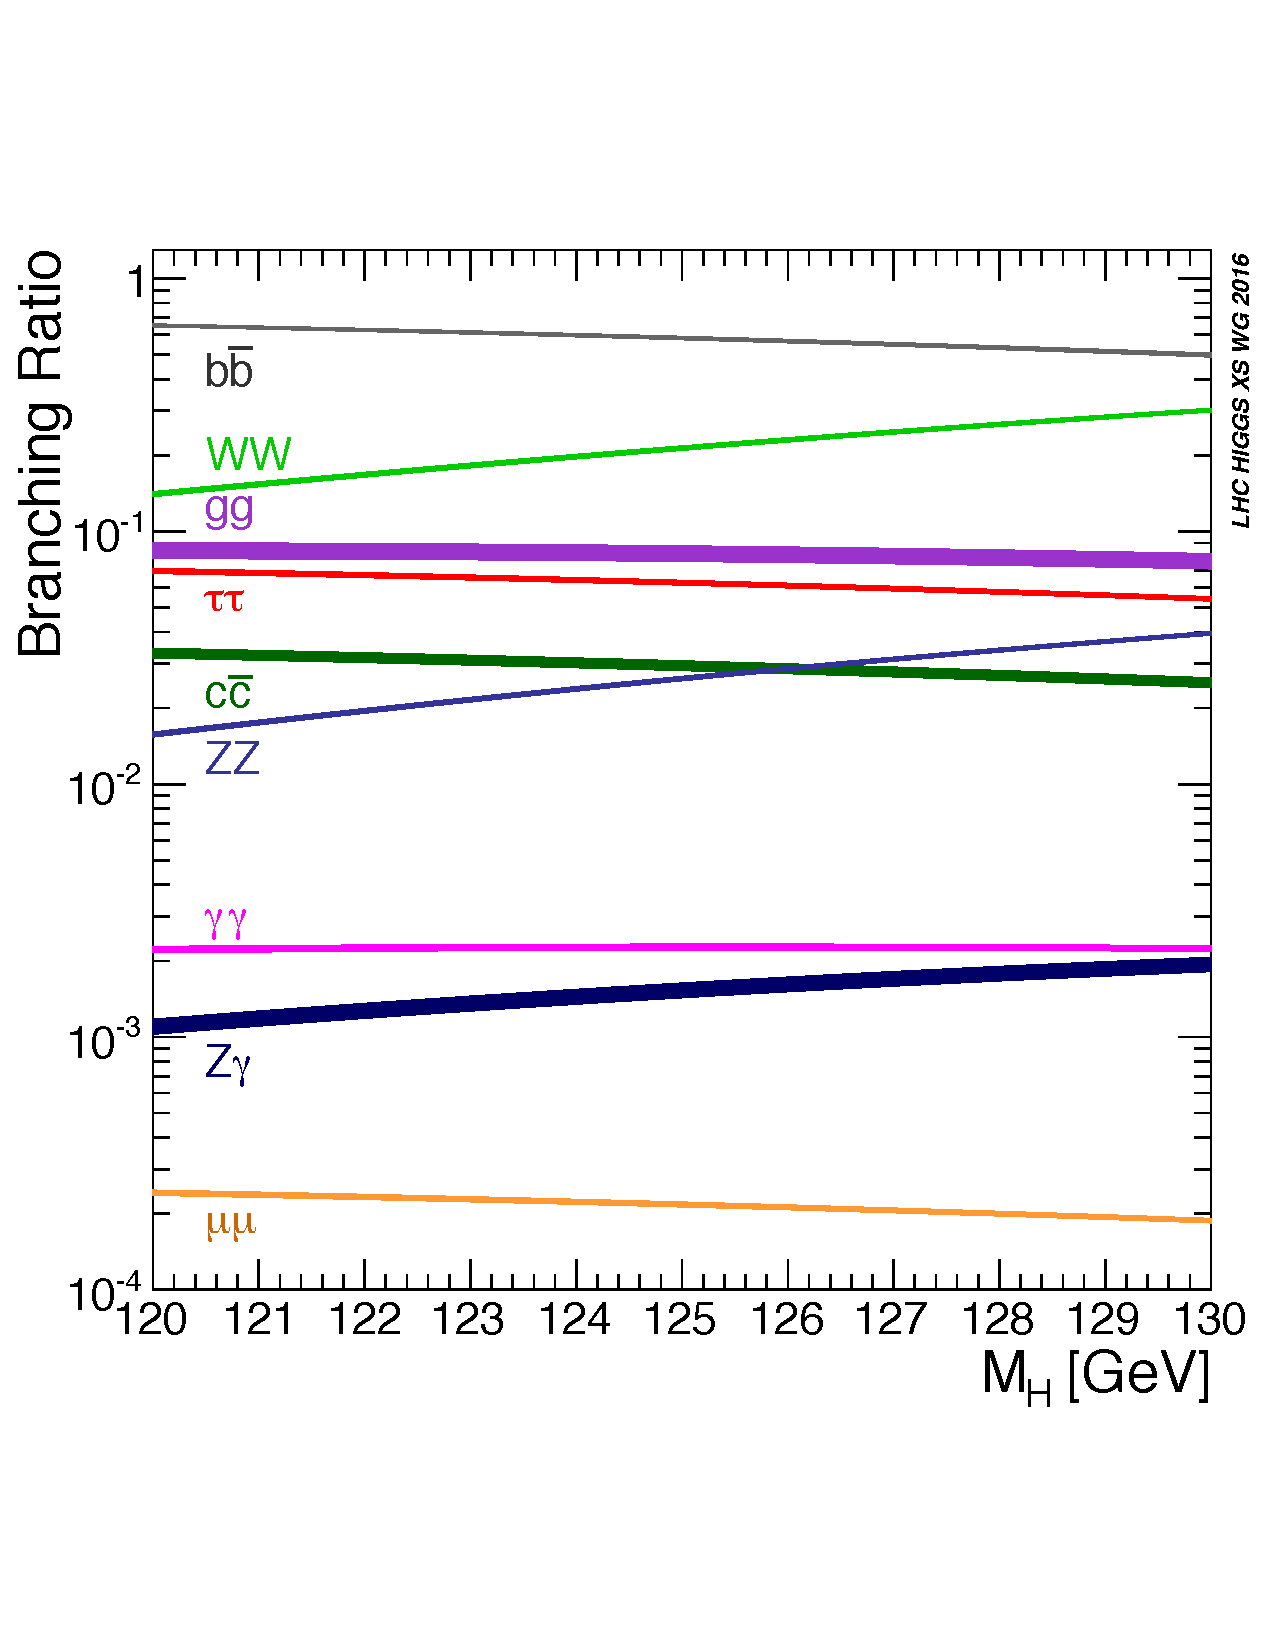
\includegraphics[width=3.5in]{images/SMHiggsBR-YR4-square}
    \caption[Higgs Boson Branching Ratios]{The branching ratios of the Higgs boson as a function of its mass \massH. \cite{CERNYR4}. The shaded bands indicate the theoretical uncertainty of the calculation while the labels indicate the decay mode.}
    \label{fig:higgsbrplots}
\end{figure}

The probability of a particular decay mode occuring is given by its \textit{branching ratio}, and is shown in Figure \ref{fig:higgsbrplots} as a function of the Higgs boson mass \massH. For a Higgs boson mass of $\massH = 125\ \GeV$, the state-of-the-art values computed for the branching ratios of its allowed decays are, in descending order,
\begin{alignat*}{2}
  &\textrm{BR}\left( H \rightarrow \bb \right) &&= 0.5824\ {}_{-0.65\%}^{+0.65\%}\ (\mathrm{theory}) {}_{-0.74\%}^{+0.72\%}\ (m_{q}) {}_{-0.80\%}^{+0.78\%}\ (\alpha_{s}), \\
  &\textrm{BR}\left( H \rightarrow \bosW\bosW \right) &&= 0.2137\ {}_{-0.99\%}^{+0.99\%}\ (\mathrm{theory}) {}_{-0.98\%}^{+0.99\%}\ (m_{q}) {}_{-0.63\%}^{+0.66\%}\ (\alpha_{s}), \\
  &\textrm{BR}\left( H \rightarrow \bosgln\bosgln \right) &&= 0.08187\ {}_{-3.41\%}^{+3.40\%}\ (\mathrm{theory}) {}_{-1.13\%}^{+1.12\%}\ (m_{q}) {}_{-3.61\%}^{+3.69\%}\ (\alpha_{s}), \\
  &\textrm{BR}\left( H \rightarrow \tau\bar{\tau} \right) &&= 0.06272\ {}_{-1.16\%}^{+1.17\%}\ (\mathrm{theory}) {}_{-0.98\%}^{+0.98\%}\ (m_{q}) {}_{-0.62\%}^{+0.62\%}\ (\alpha_{s}), \\
  &\textrm{BR}\left( H \rightarrow c\bar{c} \right) &&= 0.02891\ {}_{-1.20\%}^{+1.20\%}\ (\mathrm{theory}) {}_{-0.98\%}^{+5.26\%}\ (m_{q}) {}_{-1.25\%}^{+1.25\%}\ (\alpha_{s}), \\
  &\textrm{BR}\left( H \rightarrow \bosZ\bosZ \right) &&= 0.02619\ {}_{-0.99\%}^{+0.99\%}\ (\mathrm{theory}) {}_{-0.98\%}^{+0.99\%}\ (m_{q}) {}_{-0.63\%}^{+0.66\%}\ (\alpha_{s}), \\
  &\textrm{BR}\left( H \rightarrow \bosg\bosg \right) &&= 0.002270\ {}_{-1.72\%}^{+1.73\%}\ (\mathrm{theory}) {}_{-0.99\%}^{+0.93\%}\ (m_{q}) {}_{-0.62\%}^{+0.61\%}\ (\alpha_{s}), \\
  &\textrm{BR}\left( H \rightarrow \bosZ\bosg \right) &&= 0.001533\ {}_{-5.71\%}^{+5.71\%}\ (\mathrm{theory}) {}_{-1.01\%}^{+0.98\%}\ (m_{q}) {}_{-0.65\%}^{+0.58\%}\ (\alpha_{s}), \\
  &\textrm{BR}\left( H \rightarrow \mu\bar{\mu} \right) &&= 0.0002176\ {}_{-1.23\%}^{+1.23\%}\ (\mathrm{theory}) {}_{-0.99\%}^{+0.97\%}\ (m_{q}) {}_{-0.64\%}^{+0.59\%}\ (\alpha_{s}).
\end{alignat*}
The theoretical uncertainties account for missing higher-order QCD and electroweak corrections, while the parametric uncertainties cover the variations of the quark masses $m_{q}$, where $q = c,\ b,\ t$, and the strong coupling constant $\alpha_{s}$ which are input parameters to the calculation. The methods and theoretical treatment of the computation of these branching ratios is also documented in Ref. \cite{CERNYR4}.

\subsection{Discovery}

The discovery of a new boson with a mass close to 125 \GeV\ was announced on July 4, 2012 at CERN, with independent observations achieved by the ATLAS\cite{ATLASHiggsDiscovery} and CMS\cite{CMSHiggsDiscovery} collaborations. Within a year's time, the new particle would be verified by both experiments to have zero spin and positive parity\cite{ATLASHiggsVerify,CMSHiggsVerify} and its observed couplings would remain consistent with a Standard Model Higgs boson.\cite{HiggsCouplingConstraints} At this point, the new boson was recognized as a Higgs boson, and in 2013 the Nobel Prize in Physics would be awarded to Fran\c{c}ois Englert and Peter Higgs for their discovery of the Higgs mechanism and prediction of a Higgs boson almost half a century before its discovery.

The decay channels with the highest sensitivities were $\bosH \rightarrow \bosZ\bosZ$, with each \bosZ\ boson subsequently decaying into a pair of charged leptons, and $\bosH \rightarrow \bosg\bosg$, for which ATLAS and CMS both had observed local significances above the expected background of $3\sigma$ and $4\sigma$, respectively. While those channels individually passed the $3\sigma$ threshold for establishing evidence, it would take their combination with other channels for ATLAS to surpass and CMS to reach $5\sigma$, the threshold for declaring a discovery. By the beginning of 2015, when the LHC would resume operations since its first planned maintainence period, the Higgs production modes of gluon fusion and vector boson fusion had been observed, as well as its decays to $WW$, $ZZ$, and $\bosg\bosg$. 

\section{Searches for \VHbb}

The preferred decay mode of the Higgs boson, as determined by its measured mass of $\massH = 125.26 \pm 0.16\ \GeV$\cite{PDG2018}, is to a bottom quark-antiquark pair, henceforth \Hbb, with a branching ratio of nearly 59\%. An observation would establish clearly the coupling of the Higgs boson to bottom quarks, and to down-type quarks in general. Moreover, as the dominant decay mode, a precise measurement of its branching ratio has direct ramifications for improving the constraints on the total decay width of the Higgs boson and provides an opportunity to check for anomalous Yukawa couplings that may present a case for new physics beyond the Standard Model. The observation of \Hbb\ is therefore of great scientific interest and experiments must be dedicated towards searching for this decay.

\subsection{Motivation for \VHbb}

The experimental challenge of searching for \Hbb\ is in distinguishing its decay signature, or signal, from the immense background of Standard Model processes. The bottom and antibottom quarks produced by the decay will both hadronize due to color confinement, forming two unstable B-hadrons that subsequently decay into cones of lighter particles known as jets. Such a final state is not unique, as QCD processes which produce many jets are a common occurance. However, even if the pair of jets can be correctly identified as originating from bottom quarks and not lighter quarks or gluons, the multijet production of a bottom quark-antiquark pair occurs at a rate that is seven orders of magnitude greater than the gluon fusion production of a Higgs boson that decays into a bottom quark-antiquark pair, as shown in Figure \ref{fig:MCFM}. While advances in the field of jet substructure may eventually enable such a strategy\cite{ggHbb}, a direct search for final states containing only two \qrkb-jets faces a large and irreducible multijet background.

One solution for mitigating the multijet background is searching for \Hbb\ using the remaining Higgs boson production modes and exploiting their final state topologies. The vector boson fusion final state is fully hadronic, as the two scattering quarks will form their own jets, and is challenging in its own right. The top-quark associated production final state potentially contains leptons from the dominant decay of the top quark, $\qrkt \rightarrow \bosW\qrkb$, but a combinatorial complexity arises with the presence of additional \qrkb-jets. The key lies in using the weak vector boson associated production mode, henceforth \VHbb, which offers a final state that can be distinguished by the leptonic decays of either the \bosW\ or \bosZ\ , thereby enabling the reduction of the multijet background to negligible levels.

\begin{figure}[htbp]
  \centering
    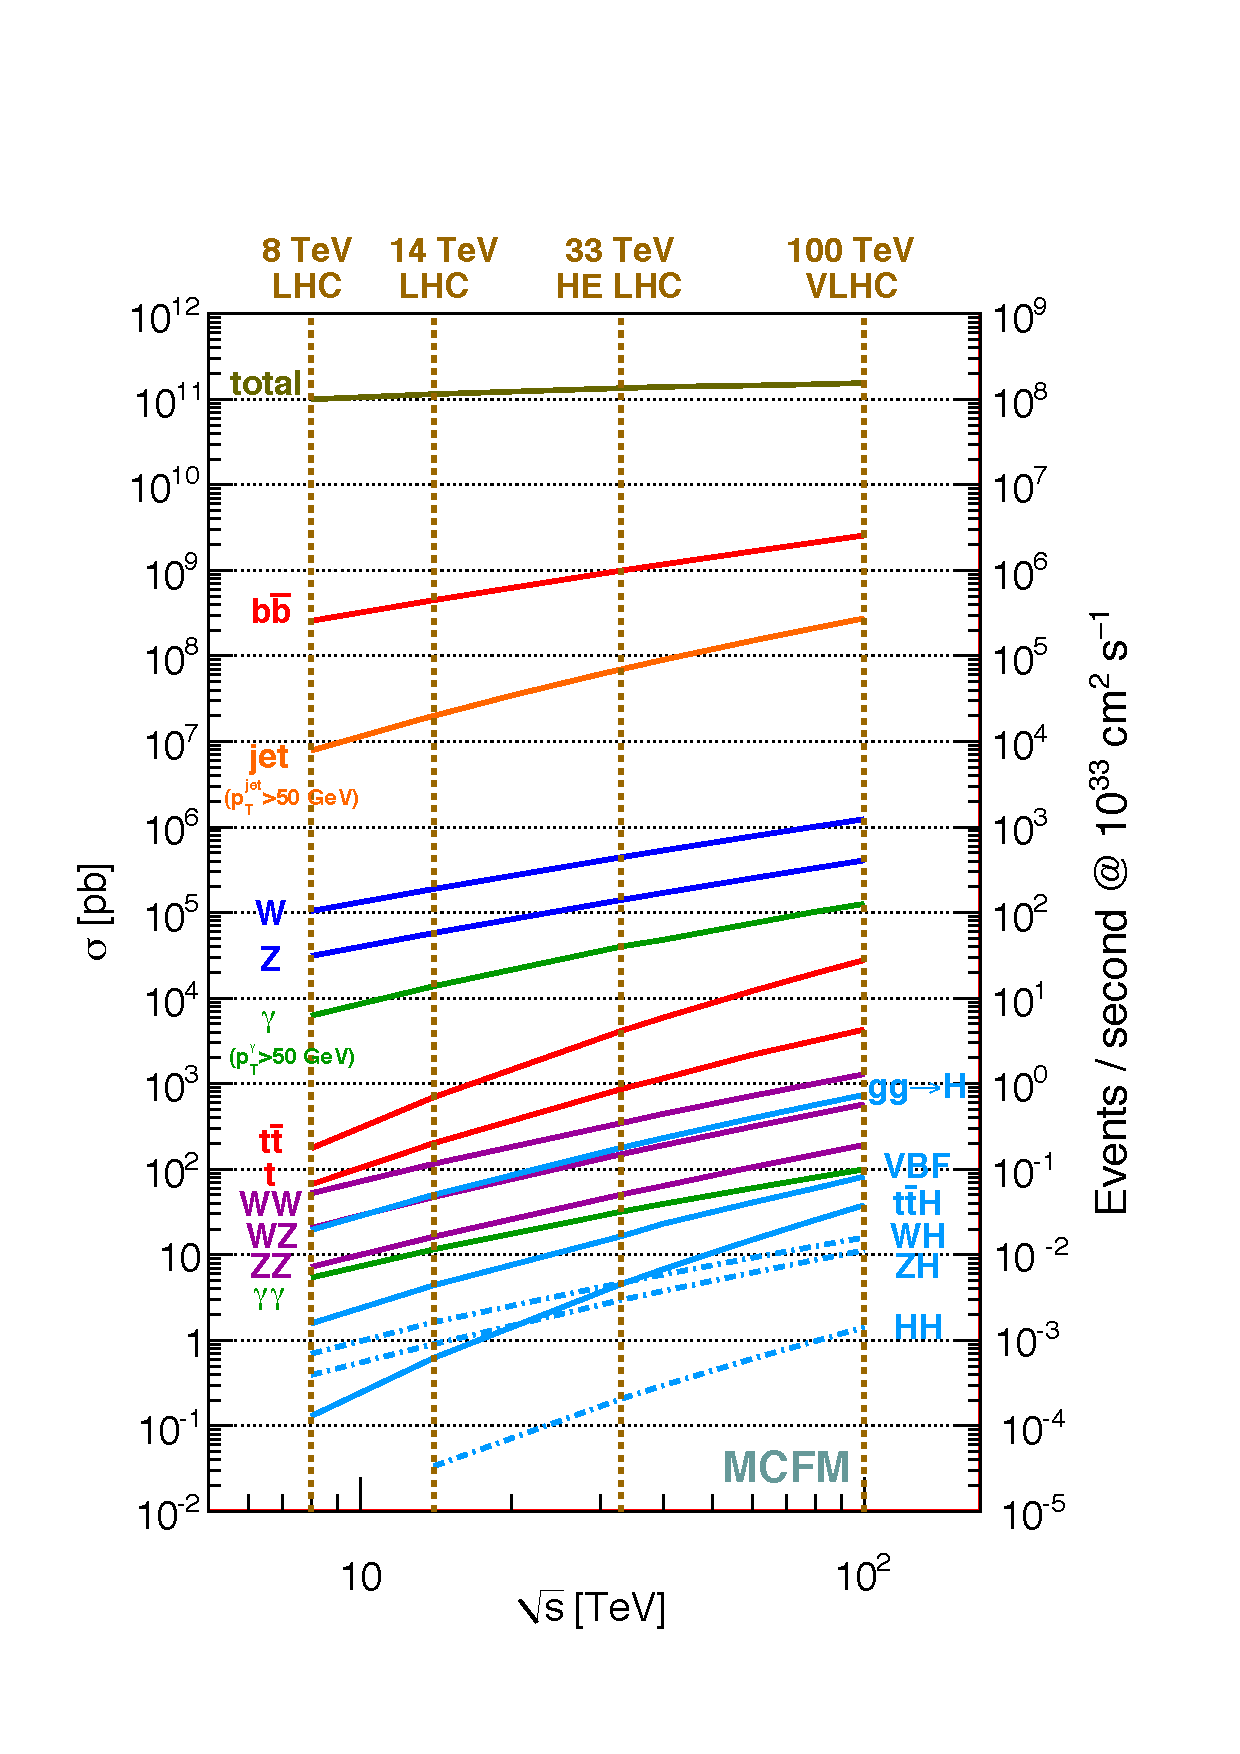
\includegraphics[width=3.5in]{images/mcfm-Edep}
    \caption[Production Cross Sections at the LHC]{The predicted production cross sections of various processes for the range of center-of-mass energies achieved and within reach at the LHC.\cite{MCFM}}
    \label{fig:MCFM}
\end{figure}

Searches based on \VHbb\ must also contend with known Standard Model background processes, such as those measured in Figure \ref{fig:SMxsec},  which mimic its final states. The main irreducible backgrounds come from \bosW\ and \bosZ\ bosons produced in association with jets, or $\bosV+\textrm{jets}$, and the production of top quark-antiquark pairs, or $t\bar{t}$, which have cross sections that are three to four orders of magnitude larger than that of \VHbb. The single top and diboson, or $\bosV\bosV$, processes are also important backgrounds, but with cross sections that are only one to two orders of magnitude larger than that of \VHbb. The Feynman diagrams for examples of these background processes are shown in Figure \ref{fig:VHbkgdiagrams}.

\begin{figure}[htbp]
  \centering
    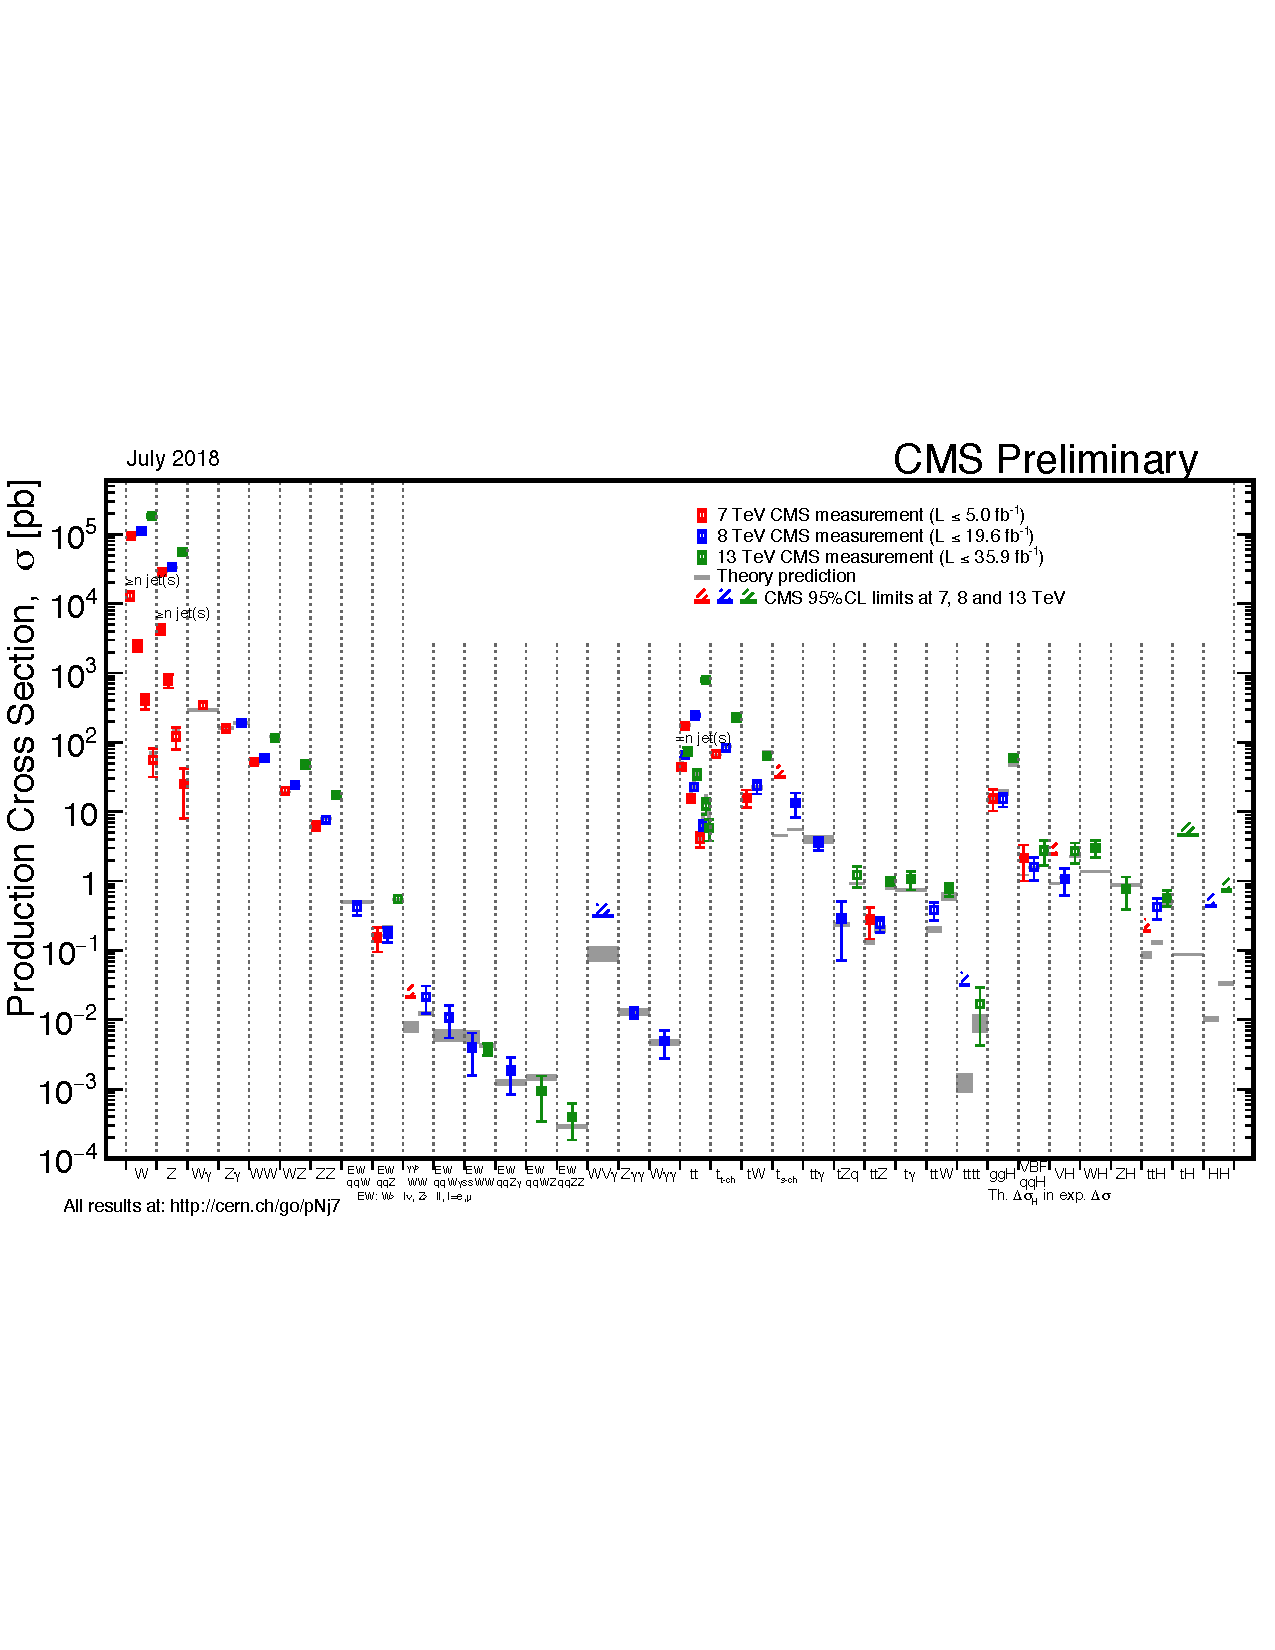
\includegraphics[width=6in]{images/SigmaNew_v0}
    \caption[CMS Measurements of SM Production Cross Sections]{Measurements of the production cross sections of the Standard Model processes by the CMS experiment.\cite{CMSSMXSEC}. The agreement with prediction holds remarkably well across the different center-of-mass energies of collisions at the LHC.}
    \label{fig:SMxsec}
\end{figure}

\begin{figure}[htbp]
  \centering
  \mbox{
    \subfigure [] {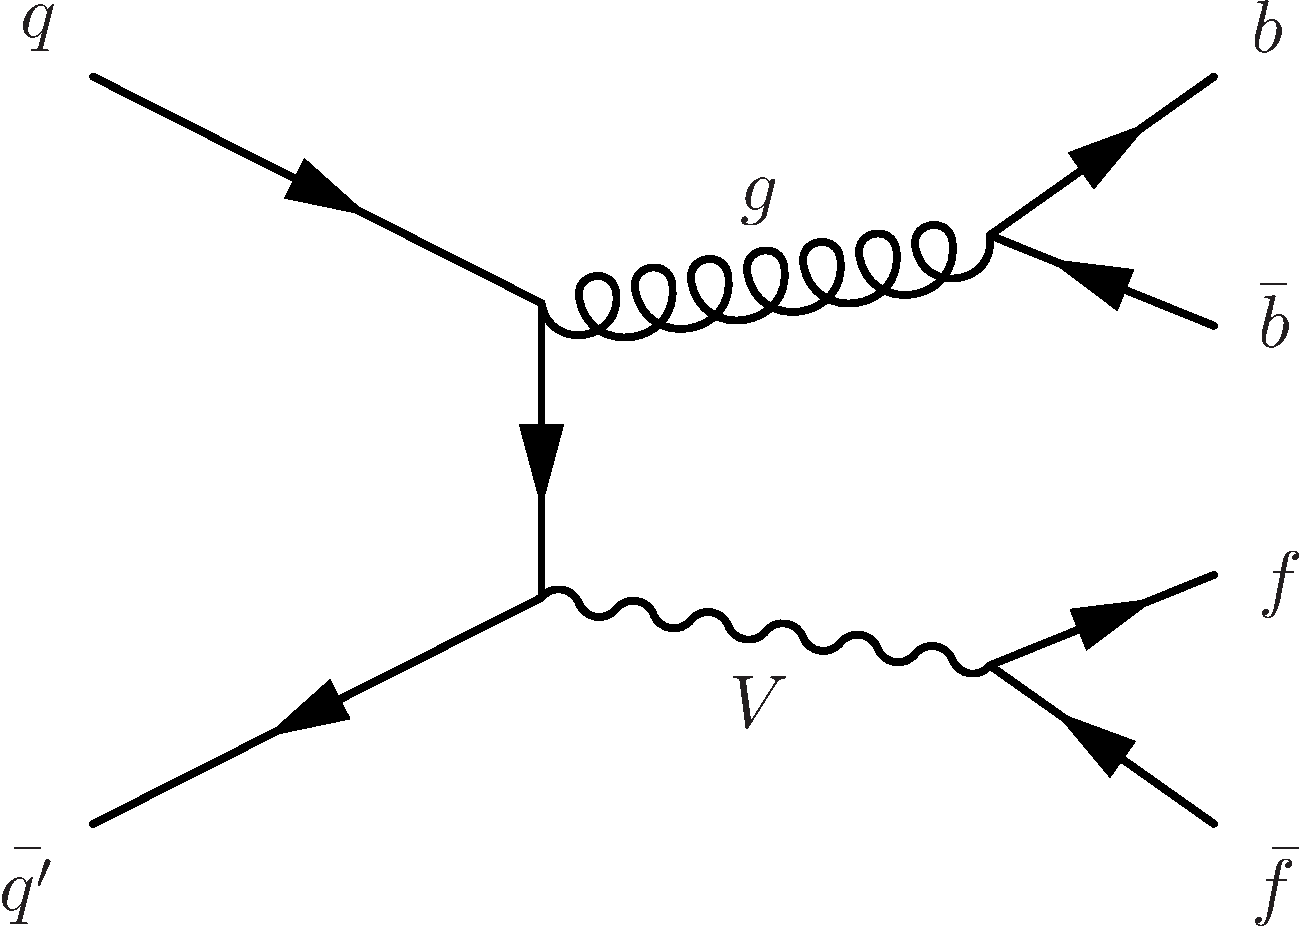
\includegraphics[scale=0.2]{images/background-Vjets}} \qquad
    \subfigure [] {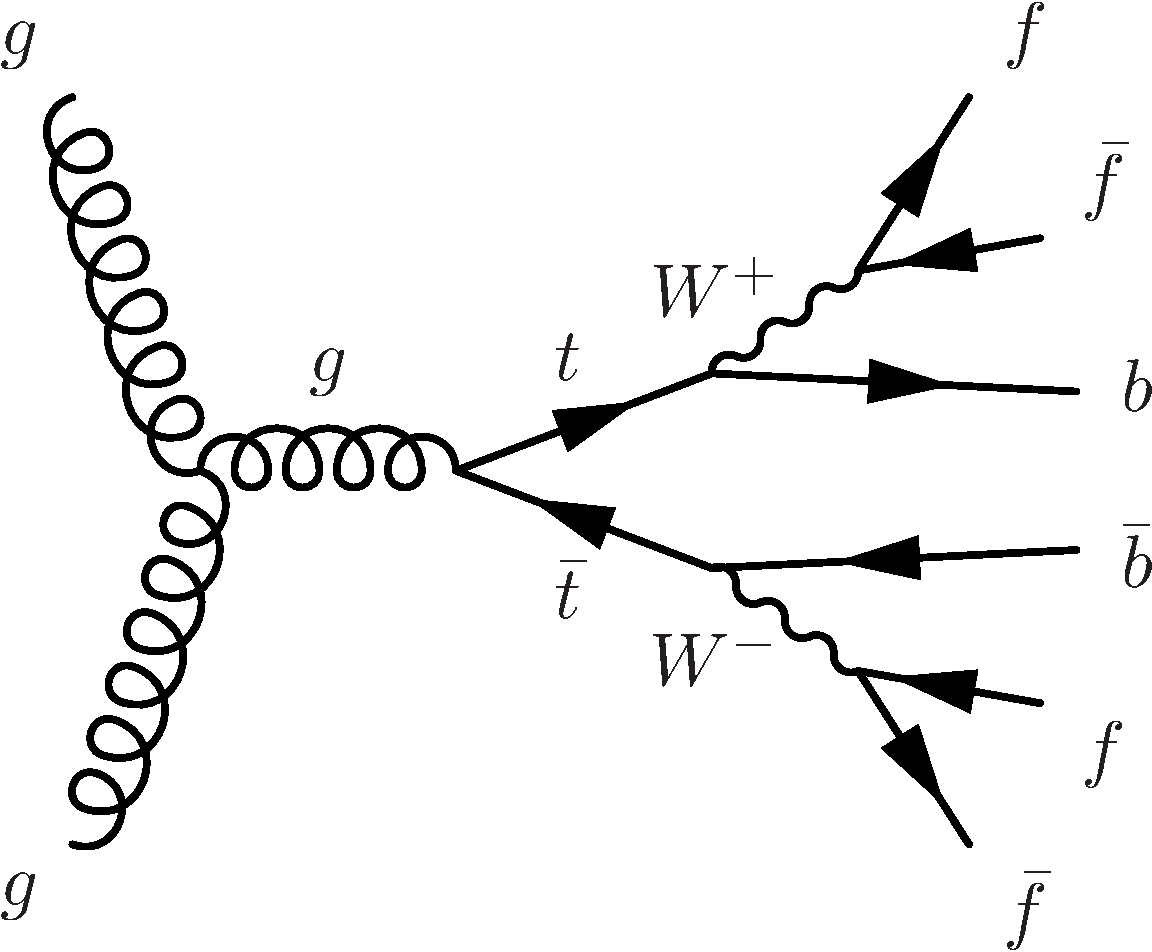
\includegraphics[scale=0.2]{images/background-tt}} \qquad
  }
  \mbox{
    \subfigure [] {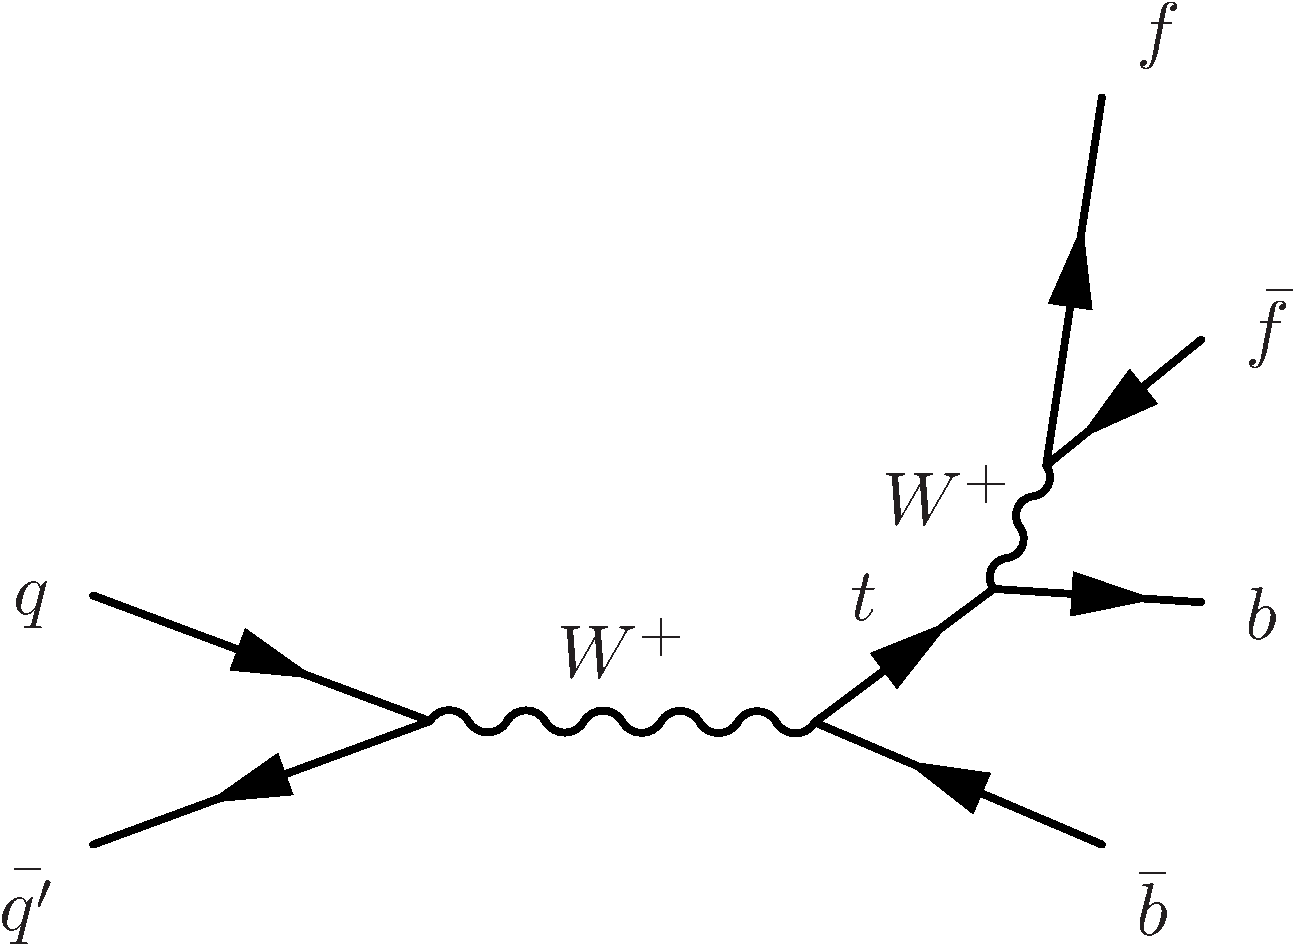
\includegraphics[scale=0.2]{images/background-top}} \qquad
    \subfigure [] {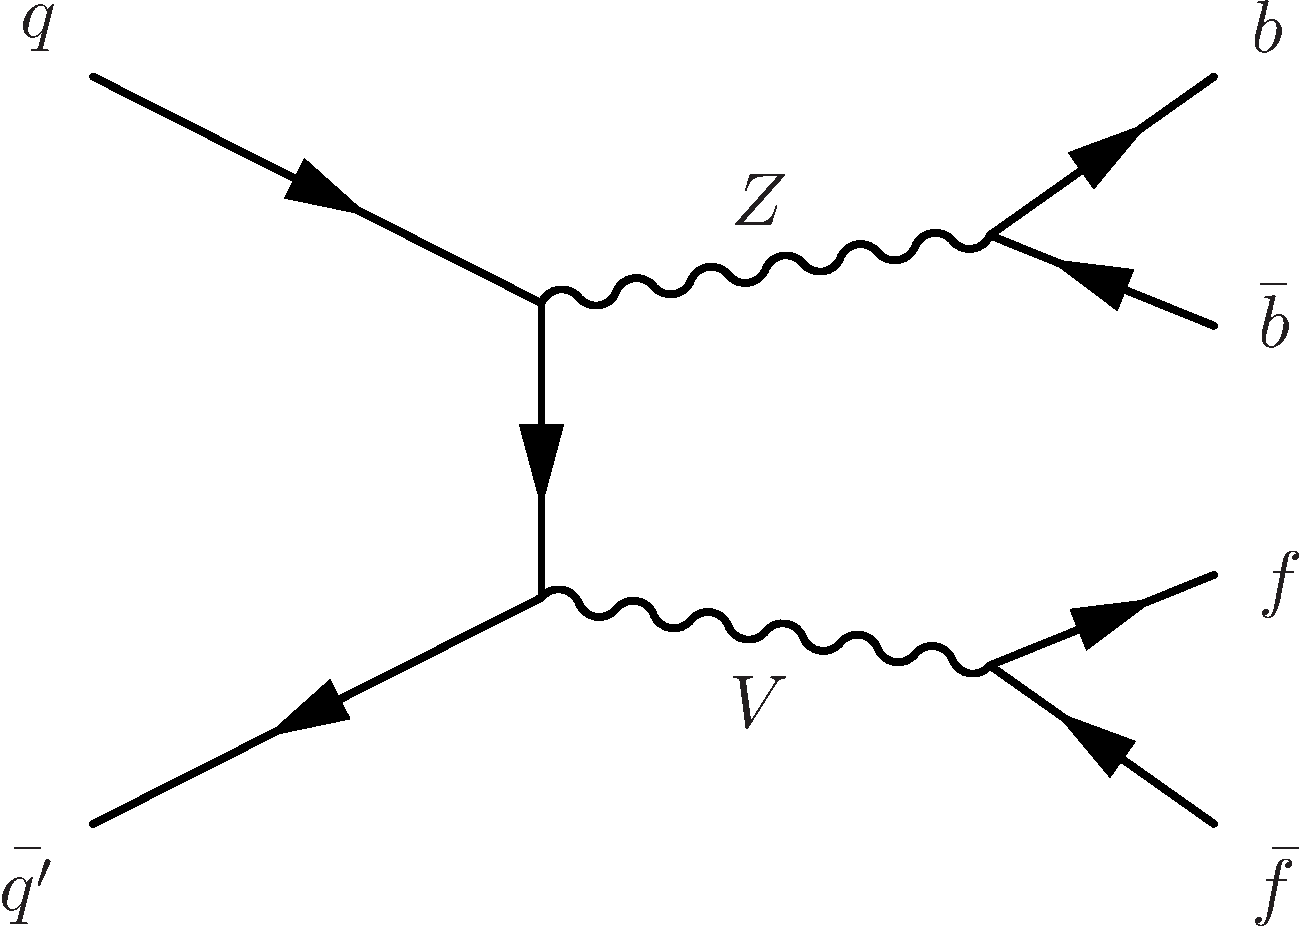
\includegraphics[scale=0.2]{images/background-VV}} \qquad
  }
  \caption[\VHbb\ Background Process Diagrams]{The Feynman diagrams for the Standard Model background processes to \VHbb. A) vector boson production in associated with jets ($\bosV+\textrm{jets}$); B) top quark-antiquark pair production ($t\bar{t}$); C) single top  D) diboson ($\bosV\bosV$).}
  \label{fig:VHbkgdiagrams}
\end{figure}

\subsection{Previous Results}

The first searches for \VHbb\ coincided with the first searches for the Higgs boson and began at the Large Electron-Positron (LEP) collider which operated from 1989 to 2000 at CERN in Geneva, Switzerland. At LEP, a Higgs boson would have been produced primarily through \bosZ\ boson associated production initiated by the annihilation of an electron-positron pair. Although the Higgs boson was not found, the four LEP experiments ALEPH, DELPHI, OPAL, and L3 analyzed the full dataset collected at center-of-mass energies above $\sqrt{s} = 189\ \GeV$\ and established a lower bound of 114.4 \GeV\ for the mass of the Higgs boson at the 95\% confidence level.\cite{LEPResult}

The first searches for \VHbb\ using hadron collisions were done at the Tevatron at Fermi National Accelerator Laboratory (FNAL) in Batavia, Illinois. The Tevatron collided protons and antiprotons at center-of-mass energies up to $\sqrt{s} = 1.96\ \TeV$\ and operated from 1985 until 2011. Although the Higgs boson was not observed, a combined analysis of the full Tevatron datasets collected by the CDF and D0 experiments yielded an observed significance of $2.8\sigma$, just shy of establishing evidence for the \VHbb\ decay.\cite{TevatronResult}

The most recent searches for \VHbb\ have taken place at the Large Hadron Collider (LHC), also located at CERN, using collisions between protons. During Run 1, which lasted from 2010 to 2013, the LHC collided protons at center-of-mass energies of $\sqrt{s} = 7\ \mathrm{and}\ 8\ \TeV$. Analysis of the Run 1 datasets were unable to obtain evidence for \VHbb\, with observed significances of $1.4\sigma$ and $2.5\sigma$ by the ATLAS and CMS experiments, respectively.\cite{ATLASVHbbRun1,CMSVHbbRun1} A combination of these results only brought the observed significance up to $2.6\sigma$.\cite{ATLASandCMSVHbbRun1}

After its upgrades during Long Shutdown 1 (LS1), the LHC resumed operations and Run 2 commenced with the center-of-mass energy of collisions increased to $\sqrt{s} = 13\ \TeV$. Although the increase in energy meant a larger cross section for \VHbb, it also led to relatively larger increases in the cross sections of the Standard Model background processes as demonstrated in Table \ref{tbl:SvsBxsec}, further complicating the search for \VHbb. However, this pessimism was unwarranted, as ATLAS and CMS both established evidence for the \VHbb\ decay by observing significances of $3.6\sigma$ and $3.8\sigma$, respectively, after combining the results of their initial Run 2 and Run 1 analyses.\cite{ATLASVHbbEvidence,CMSVHbbEvidence}

\begin{table}[htbp]
  \caption[Production Cross Sections for the Higgs Boson and SM Background Process at the LHC]{A list of Higgs boson and Standard Model background production cross sections at center-of-mass energies of $\sqrt{s} = 8\ \mathrm{and}\ 13\ \TeV$, along with the relative increase at $\sqrt{s} = 13\ \TeV$.}
  \label{tbl:SvsBxsec}
  \begin{tabularx}{6.5in}{XXXX}
    \hline
    Cross Section                                  & $\sqrt{s} = 8\ \TeV$ & $\sqrt{s} = 13\ \TeV$ & Relative Increase at $\sqrt{s} = 13\ \TeV$ \\
    \hline
    $\sigma\left( pp \rightarrow H \right)$        & 19.4 \pb             & 44.1 \pb              & 2.27                                       \\
    $\sigma\left( pp \rightarrow qqH \right)$      & 1.6 \pb              & 3.8 \pb               & 2.38                                       \\
    $\sigma\left( pp \rightarrow VH \right)$       & 1.23 \pb             & 2.26 \pb              & 1.84                                       \\
    $\sigma\left( pp \rightarrow ttH \right)$      & 133 \fb              & 507 \fb               & 3.81                                       \\
    $\sigma\left( pp \rightarrow t\bar{t} \right)$ & 253 \pb              & 832 \pb               & 3.29                                       \\
    \hline
  \end{tabularx}
\end{table}

Naive projections assuming increased statistics and similar systematic uncertainties suggested that an observation of \VHbb\ may be possible if the experimental sensitivty could be improved by about 20\%. With Run 2 on track to produce more data in 2017 than 2016, such a historic result appeared to be on the horizon. The analysis of the 2017 dataset and the results obtained by the CMS experiment are the subject of this dissertation.

%We don't make the Chapter titles in All Caps Automatically because it is easier for you to type your Chapter Titles in uppercase than for those that need to have mixed case in their titles to find the correct command in the ufthesis.cls file and change it there. \renewcommand*{\thefootnote}{\fnsymbol{footnote}}\footnote{an un-numbered footnote - this is how you tell the readers that this chapter was previously published and then cite the Journal where it was published} We don't recommend that you change much of anything in the class file unless you're absolutely sure of what your are doing.\renewcommand*{\thefootnote}{\arabic{footnote}}\setcounter{footnote}{0}\footnote{and now we're back to normal footnote marking}

%Title case is where all principal words are capitalized except prepositions, articles, and conjunctions.  %\cite{green2008wrinkle}

%\subsection{Subsection Commands Are Also in Title Case}
%The difference, of course, are the second level headings are left-aligned
%
%\subsubsection{Subsubsections are in sentence case}
%The third level subheadings are left-aligned but in sentence case. Only the first letter and any proper nouns are capitalized. %\cite{strickler1998contamination}
%
%\subsubsection{If you divide a section, you must divide it into two, or more, parts}
%
%{\bf Paragraph headings.} There is no official fourth level heading. Do not use the Paragraph heading feature in LaTeX, simply apply the bold characteristic to the first few words of a paragraph followed by a colon or period.

%\subsection{I Need Another Second Level Heading in This Section}
%
%Aliquam mi nisi, tristique at rhoncus quis, consectetur non mi. Phasellus blandit quam ligula, a viverra lacus commodo at. In iaculis nisl vel pretium sollicitudin. In efficitur massa vel elit sollicitudin, vel auctor sapien cursus. Proin feugiat sapien a mi tempus;
%
% $ X-X'=D+D'$
%
% in consequat augue cursus. Nulla sed sagittis purus. Nunc eu consequat orci, eu laoreet enim. Ut euismod tincidunt sem, eget lacinia dui luctus eu. Aliquam mi augue, faucibus id semper vitae, porta ac ligula. Morbi sed ultrices odio. Mauris id luctus ex. Nulla ac libero dictum, interdum turpis lacinia, scelerisque leo. Praesent varius orci ac eros varius pharetra.
%
%\section{Image Handling in XeLaTeX}
%
%One of the biggest reasons for switching from the dvipdfm/dvipdfmx methods of compiling is the improved image handling capabilities. EPS, Bit-mapped, PDF, JPG, and PNG formats work well with the xelatex process.
%
%\subsection{The Traditional EPS Format}
%
%EPS format is the traditional format for LaTeX, but EPS files can be very large and many programs can't create or view these images. There are many programs that are used to interpret data and output the results as an EPS format image. It has been my experience that there are bounding box problems with these figures. On many occasions we have opened the image in Adobe Photoshop and, without making any changes, saved the document as a Photoshop EPS file, re-compiled the document, and the image worked correctly, so if you are having problems with an EPS image not showing in your document correctly, try this fix first.
%
%
%\begin{figure}[htbp]
%  \centering
%    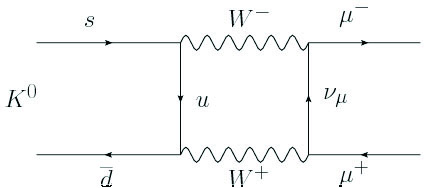
\includegraphics[width=5in]{images/diagram}
%    \caption[EPS format diagram. Note: no filetype is designated by adding an extension.]{EPS format diagram. Note: no filetype is designated by adding an extension. The file type is determined and the correct procedure is automatically chosen by xelatex.}
%\end{figure}
%
%
%Quisque malesuada a leo eget ullamcorper. Curabitur ut aliquam quam. Nam quis quam id mauris aliquam blandit porttitor sit amet quam. Donec ut erat eleifend turpis finibus pulvinar.
%
%\subsection{Bitmapped Images Work As Well}
%
%Bitmapped images are a standard file type on PCs, but these files are also usually very large so compressed images may be a better alternative.
%
%\begin{figure}[htbp]
%  \centering
%    \includegraphics[width=5in]{images/eagle}
%    \caption[BMP format drawing. Note: no filetype is designated by adding an extension.]{BMP format drawing. Note: no filetype is designated by adding an extension. The file type is determined and the correct procedure is automatically chosen by xelatex.}
%\end{figure}
%
%Morbi hendrerit risus nec quam posuere viverra. Donec quis tellus faucibus, molestie arcu sed, congue urna. Duis eget neque ac libero pulvinar porta eget et magna. Donec a magna eu eros suscipit cursus ac vitae nisl. Vivamus ligula purus, congue sed tortor blandit, ultrices egestas nisl.
%
%\subsection{Not to Mention PDF}
%
%It is often very handy to be able to include a pdf file as an image. By using XeLaTeX this is usually just matter of setting the size, or scale properties correctly.
%
%\begin{figure}[htbp]
%  \centering
%    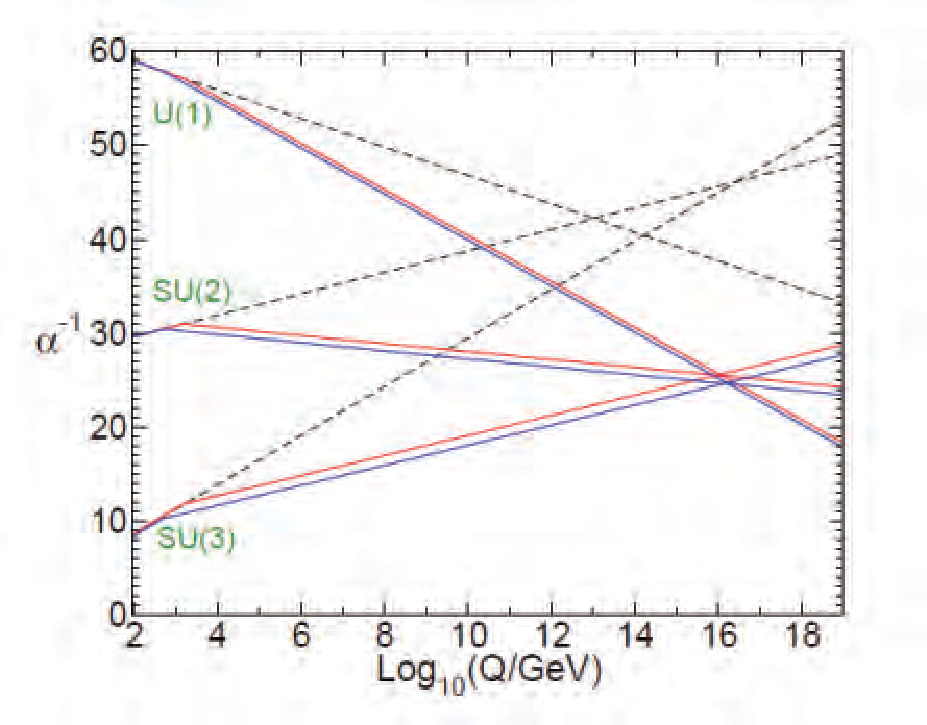
\includegraphics[scale=1.0]{images/graph.pdf}
%    \caption[PDF format graph. Note: no filetype is designated by adding an extension.]{PDF format graph. Note: no filetype is designated by adding an extension. The file type is determined and the correct procedure is automatically chosen by xelatex.}
%\end{figure}
%
%Nulla mattis augue lacus. Nam non lectus dolor. Cras ac quam vel justo elementum vestibulum. Integer vulputate pulvinar lacus sit amet pulvinar.
%
%\subsection{JPG Is Absolutely Necessary}
%
%For photographs, JPG is the most common format. This format is a fraction of the size of Bit-mapped images and can deliver very good quality at a much smaller overhead. Vestibulum eu lectus vel orci dictum vehicula. Proin id maximus dolor. Integer augue ante, pulvinar ac erat vitae, porttitor ullamcorper libero. %\cite{l2012wrinkle}
%
%\begin{figure}[htbp]
%  \centering
%    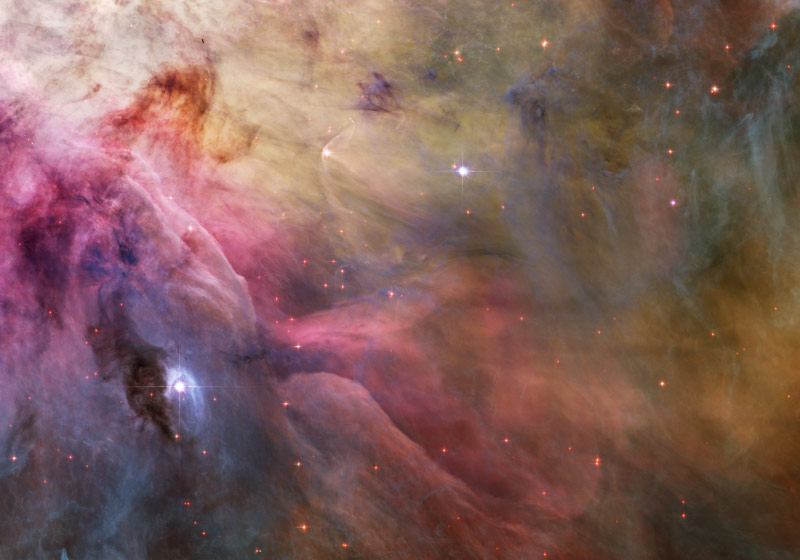
\includegraphics[width=5in]{images/nebula}
%    \caption[JPG format image. Note: no filetype is designated by adding an extension.]{JPG format image. Note: no filetype is designated by adding an extension. The file type is determined and the correct procedure is automatically chosen by xelatex.}
%\end{figure}
%
%Nunc blandit scelerisque velit, ac facilisis dui finibus et. Sed facilisis tortor vel commodo luctus. Donec est felis, malesuada id nibh in, accumsan malesuada lectus. Sed lobortis volutpat felis, vitae aliquet augue congue id. Fusce ut odio tincidunt, condimentum nulla vel, pharetra arcu.
%
%\subsection{PNGs Will Help Make Files Smaller}
%
%PNG files are even smaller than JPGs and are very good when text and images are combined.
%
%\begin{figure}[htbp]
%  \centering
%    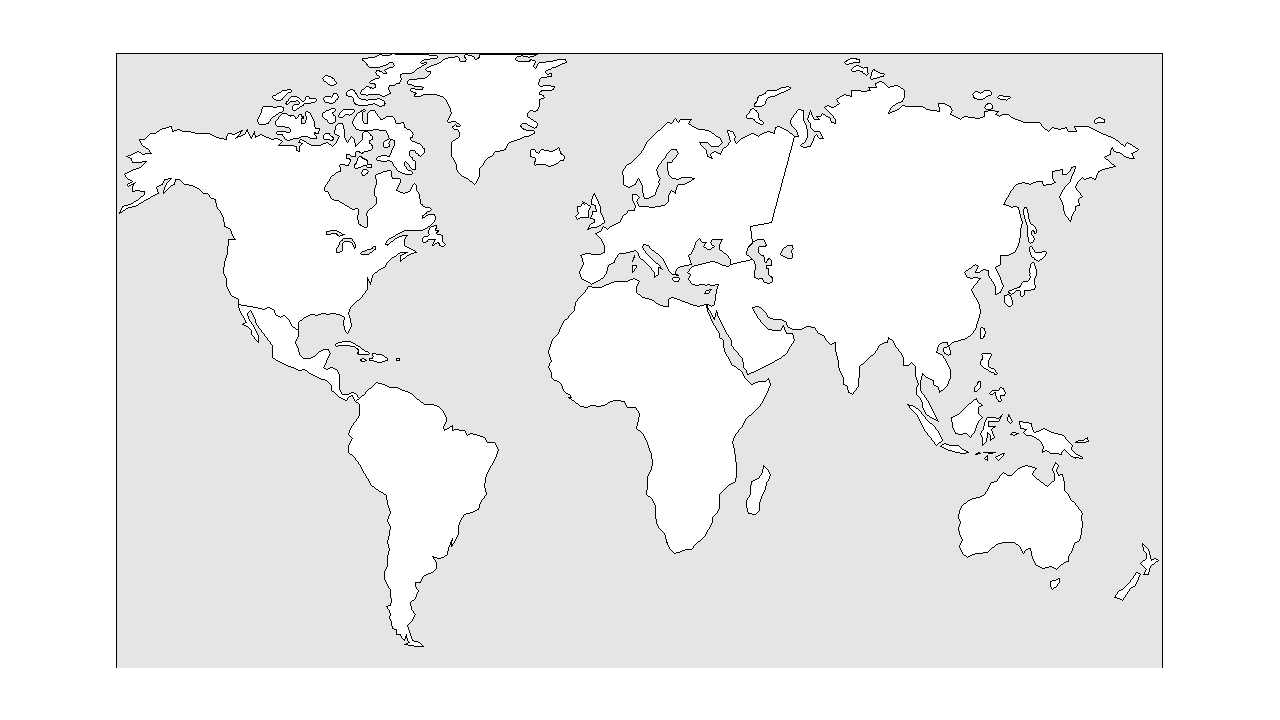
\includegraphics[width=5in]{images/theworld}
%    \caption[PNG format map. Note: no filetype is designated by adding an extension.]{PNG format map. Note: no filetype is designated by adding an extension. The file type is determined and the correct procedure is automatically chosen by xelatex.}
%\end{figure}
%
%
%
%Aenean condimentum libero sed mi porta, tempus ullamcorper lectus venenatis. Aliquam in diam dolor. Maecenas tempus consectetur sem et pulvinar. Aenean aliquam at metus ut hendrerit. Vivamus molestie ac neque eu luctus. Nam convallis maximus quam non lobortis. Fusce sit amet lorem et massa convallis aliquet at sit amet nulla. Suspendisse nec ex elit. Aenean gravida, sapien vitae congue commodo, urna turpis ornare libero, at cursus risus libero in erat. %\cite{Rust94}
%
%\section{GIF, TIF, and Others}
%
%Other file formats have not been successful, with or without file extensions. The tests have not been exhaustive so if you have a different type, give it a try. GIF, and TIF both do NOT work at this time. The next image demonstrates how to use multiple images as a single figure. Notice, there is a single caption for ALL figures and that caption starts with a discription of the ENTIRE figure before breaking off into the subfigure descriptions.
%
%\begin{figure}[htbp]
%     \centering
%   \mbox{
%      \subfigure [] {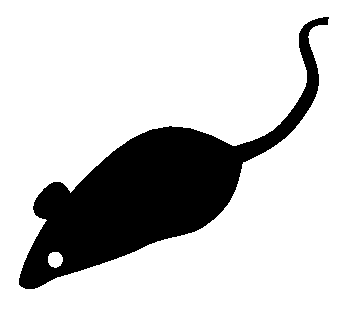
\includegraphics[scale=0.6]{images/mouse}} \qquad
%      \subfigure []{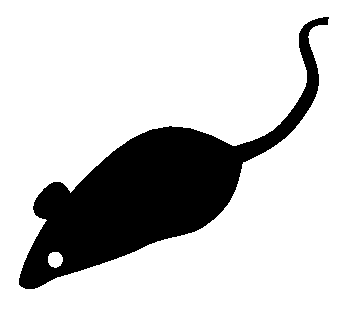
\includegraphics[scale=0.6]{images/mouse}} \qquad
%     }
%    \mbox{
%      \subfigure [] {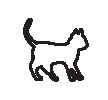
\includegraphics[scale=3]{images/cat}} \qquad
%      \subfigure [] {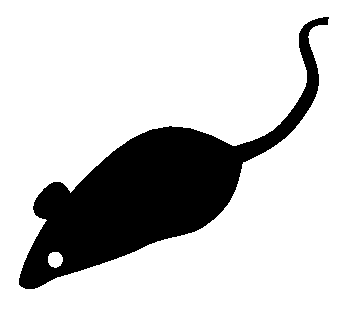
\includegraphics[scale=0.6]{images/mouse}} \qquad
%      }
%    \caption[Tom and Jerry]{Tom and Jerries. This caption demonstrates how the sub-captions are left out of the List of Figures, but included in the figure itself. A) Tom the first; B) Tom the second; C) Jerry; D) Tom the third.}
%    \label{mice}
%  \end{figure}
%
%
%Aliquam mi nisi, tristique at rhoncus quis, consectetur non mi. Phasellus blandit quam ligula, a viverra lacus commodo at. In iaculis nisl vel pretium sollicitudin. In efficitur massa vel elit sollicitudin, vel auctor sapien cursus. Proin feugiat sapien a mi tempus, in consequat augue cursus. Nulla sed sagittis purus. Nunc eu consequat orci, eu laoreet enim. Ut euismod tincidunt sem, eget lacinia dui luctus eu. Aliquam mi augue, faucibus id semper vitae, porta ac ligula. Morbi sed ultrices odio. Mauris id luctus ex. Nulla ac libero dictum, interdum turpis lacinia, scelerisque leo. Praesent varius orci ac eros varius pharetra.
%
%
%
%Nunc blandit scelerisque velit, ac facilisis dui finibus et. Sed facilisis tortor vel commodo luctus. Donec est felis, malesuada id nibh in, accumsan malesuada lectus.
%\begin{itemize} %
%    \item WinEDT: This text editor is recommended for use editing \TeX-files as it has many useful built in macros and is easy to use  %
%    \item This program can be found and downloaded here: \url{http://www.winedt.com/} %
%    \item The GIMP (GNU Image Manipulation Program) %
%    \begin{itemize}%
%        \item A freeware graphics editing program for picture editing and file conversions %\vspace{-12pt}%
%        \item Comparable to Adobe Photoshop %\vspace{-12pt}%
%        \item Can be downloaded here: \url{http://www.gimp.org/}%
%    \end{itemize}
%    \item A good reference of \LaTeX 2\ensuremath{\epsilon} commands%
%    \begin{itemize}
%        \item This should be included on the ETD website here: \url{http://etd.helpdesk.ufl.edu/tex.php}
%    \end{itemize}
%\end{itemize} %
%
%
%Sed lobortis volutpat felis, vitae aliquet augue congue id. Fusce ut odio tincidunt, condimentum nulla vel, pharetra arcu. In ultricies libero diam, nec rutrum magna vehicula nec. Praesent dictum eros sit amet turpis ultricies, eleifend condimentum dui imperdiet. Donec congue urna ante, id rutrum mi commodo a. Vivamus id tincidunt nunc. Morbi id lacus ut augue ultricies convallis. Duis a lectus quis ante pretium scelerisque nec nec nisi. In id porta justo, at euismod diam. Suspendisse vel tempus arcu. Praesent vel cursus nisi, ac rhoncus odio.


\chapter{EXPERIMENTAL APPARATUS} \label{experiment}

It is nature's irony, that the study of subatomic particles requires the largest and most intricate machines known to date in human history. Because the physics of such particles are described by their interactions, high energy physics experiments typically accelerate particles to extreme kinetic energies, collide them against each other or dense targets, and infer the details of their interaction from the resulting final state particles. Such collisions can be \textit{elastic}, where the interacting particles merely exchange energy and remain unchanged, or \textit{inelastic}, where the interaction changes the incoming particles and has a chance of creating new, massive particles because of the time-energy uncertainty relation. Collisions of the latter kind are thus of great interest to experimentalists in the search for new particles and their decays.

Under the consideration of providing as much energy as possible towards the interaction, modern experiments favor colliding beams over fixed-target experiments. By momentum conservation, some of the energy of a fixed-target collision must be converted into the kinetic energies of final state particles, while there is no such constraint for colliding beams. Thus, at high energies, the dependence of the center-of-mass energy $\sqrt{s}$ on the incoming beam energy $E_{\textrm{beam}}$ in the laboratory frame scales as $\sqrt{s} \propto E_{\textrm{beam}}^{1/2}$ for fixed-targets, whereas it scales linearly for colliding beams $\sqrt{s} \propto E_{\textrm{beam}}$. Because the center-of-mass energy of the collision fixes the energy available for the production of new particles, colliding beams hold the advantage.

Modern experiments also favor circular rather than linear particle accelerators. Because the length of a linear accelerator is correlated with its maximum beam energy, the size required to probe the current energy frontier is prohibitively large, and even then particles can only be accelerated once through the machine. Instead, circular colliders can accelerate particles for multiple orbits until they reach the desired energy scale, and this circulation also allows for the same beams to be collided multiple times to achieve a \textit{luminosity}, a measure of particle flux, that is higher than linear accelerators. The problem faced by circular colliders is synchrotron radiation, where charged particles accelerated along a circular trajectory lose energy. Because a particle's energy loss due to synchrotron radiation is inversely proportional to the fourth power of its particle's mass, electron beams experience incredible energy losses compared to proton beams. For this reason, modern experiments prefer the acceleration and collision of hadron beams.

\section{The Large Hadron Collider}

The Large Hadron Collider (LHC) at CERN is the culmination of contemporary high energy experiment sensibilities. The world's largest machine, it is a circular accelerator with a circumference of 27 km, spanning across the Franco-Swiss border, and is housed within an underground tunnel at an average depth of 100 m. An illustration is provided in Figure \ref{fig:LHCoverallview}. It features two parallel evacuated beam pipes in which proton beams circulate in opposite directions. Although the design energy of each proton beam is 7 \TeV, the beams are currently circulating at an energy of 6.5 \TeV\ to give a center-of-mass energy of 13 \TeV\ for the one billion proton collisions it produces per second.

\begin{figure}[htbp]
  \centering
    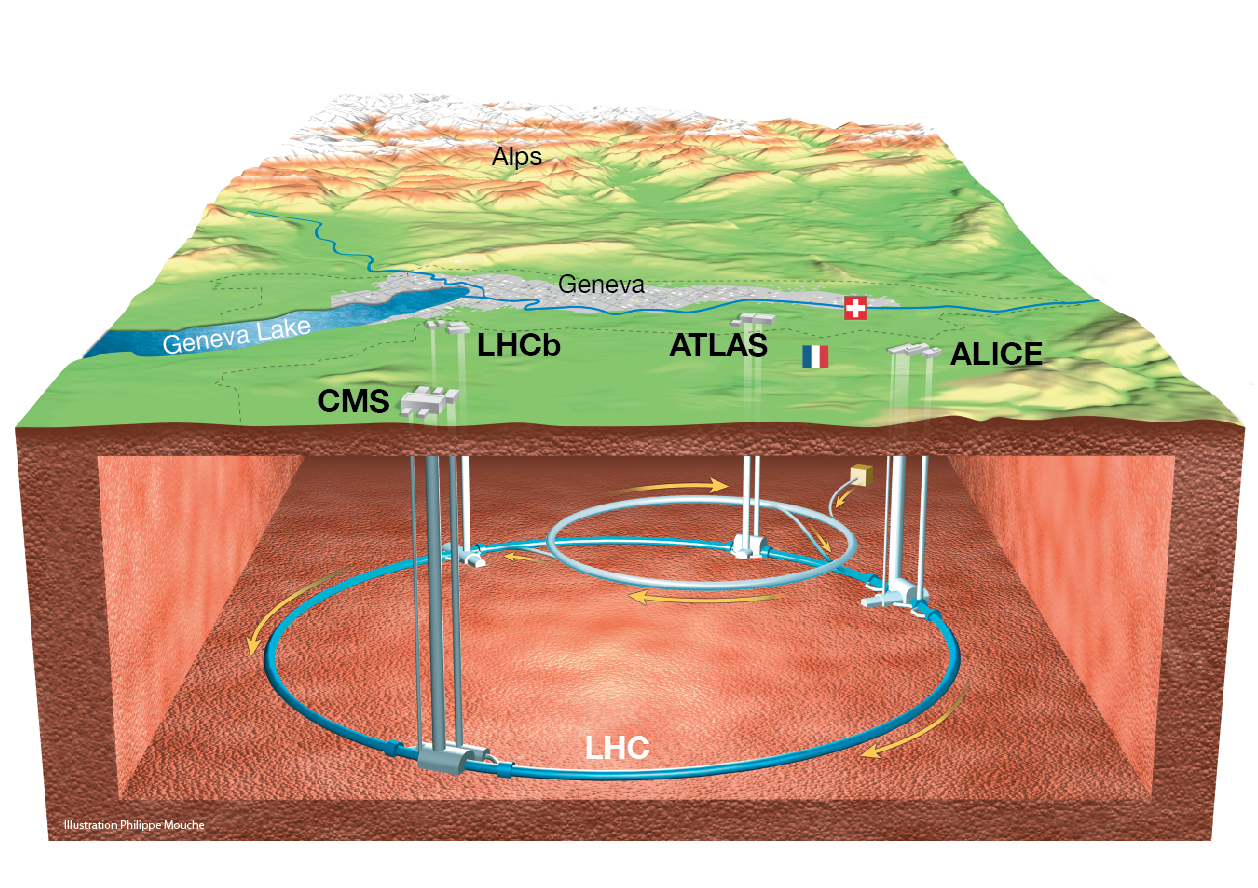
\includegraphics[width=4in]{images/LHC-illustration}
    \caption[Overall View of the LHC]{An overall view of the LHC showing the underground tunnel and its experiments in relation to its geography.\cite{LHCoverallview}}
    \label{fig:LHCoverallview}
\end{figure}

Because the LHC reuses the tunnels of the Large Electron-Positron (LEP) Collider, additional excavation was avoided and it was integrated as the final stage of CERN's accelerator complex, shown in Figure \ref{fig:CERNcomplex}. The source of protons is a canister of hydrogen gas to which a strong electric field is applied to strip the electrons from the hydrogen nuclei. The protons then pass through the linear accelerator LINAC2 and are accelerated to an energy of 50 \MeV. They are then injected into successive circular accelerators: the Proton Synchrotron Booster which accelerates the beams to 1.4 \GeV, the Proton Synchrotron (PS) which accelerates the beams to 25 GeV, the Super Proton Synchrotron (SPS) which further accelerates the beams to 450 \GeV, and finally the LHC itself. The oscillating radio frequency (RF) fields used to accelerate the protons results in beams composed of proton \textit{bunches} as opposed to a continuous stream. The LHC currently circulates up to 2556 bunches per beam, which is not far from its design value of 2808 bunches per beam.

\begin{figure}[htbp]
  \centering
    \includegraphics[width=6.5in]{images/CERNcomplex}
    \caption[The CERN Accelerator Complex]{A complete schematic of the CERN accerlator complex and experiments.\cite{CERNcomplex}}
    \label{fig:CERNcomplex}
\end{figure}

The circular orbit of the proton beams are maintained by the 1,232 bending magnets lining the LHC. The bending magnets are superconducting dipole magnets which generate 8.3 T magnetic fields powerful enough to bend the high energy beams. In order to minimize the oscillation of the bunches around their trajectories and achieve high luminosity, 392 focusing magnets are also placed along the LHC ring. The focusing magnets are superconducting quadrupole magnets with a magnetic field gradient of 223 T/m. They are placed in alternating pairs to account for their nature of focusing along one direction while defocusing the orthogonal direction. Schematics for these two main types of magnets are shown in Figure \ref{fig:lhcmagnets}

\begin{figure}[htbp]
  \centering
  \mbox{
    \subfigure [] {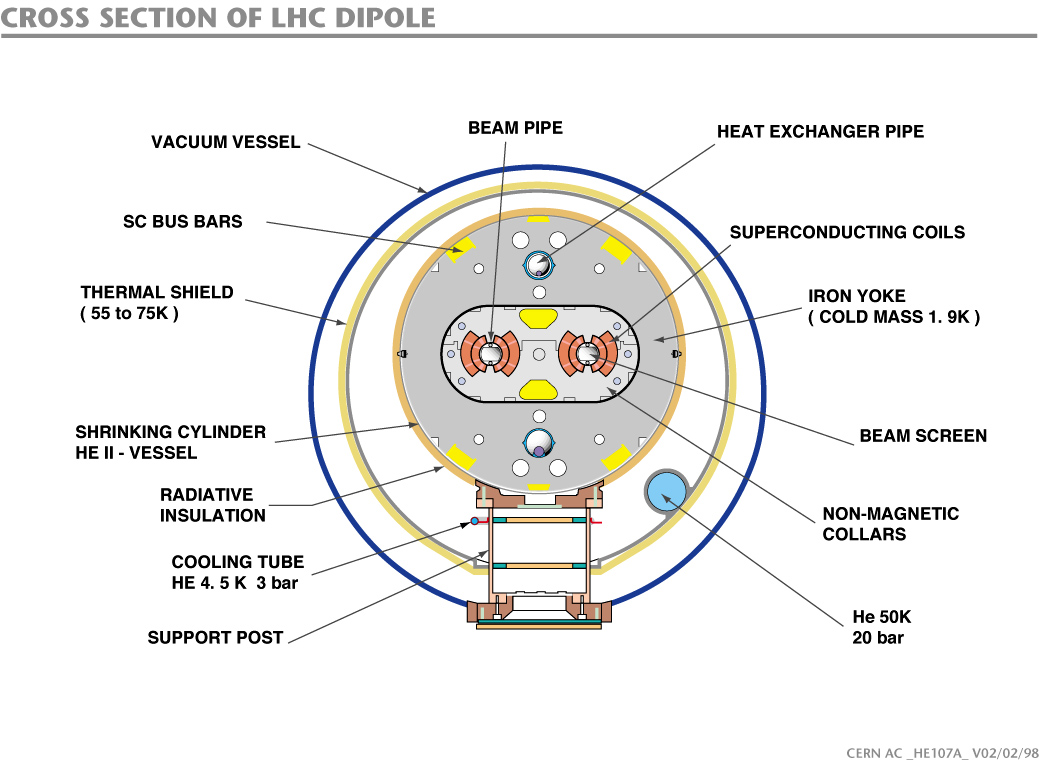
\includegraphics[scale=0.27]{images/lhc-pho-1998-341}} \qquad
    \subfigure [] {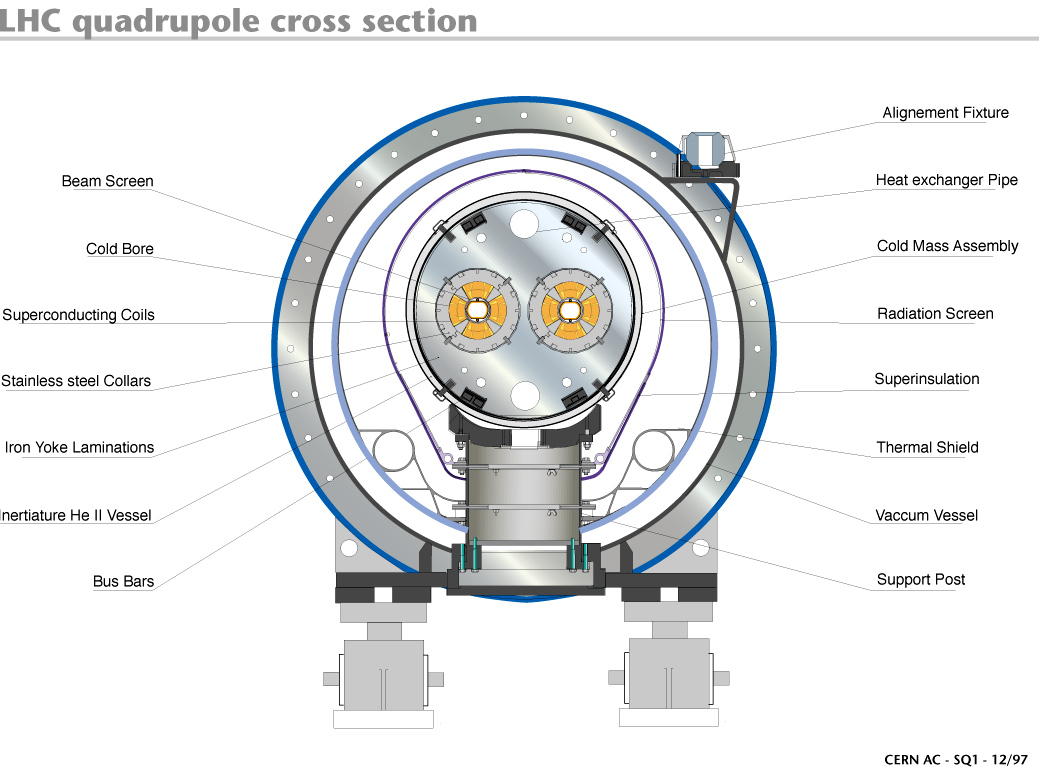
\includegraphics[scale=0.27]{images/lhc-pho-1998-312}} \qquad
  }
  \caption[LHC Dipole and Quadrupole Magnets]{The cross sectional views for the main types of LHC magnets: A) dipole magnet used for bending the beams; B) quadrupole magnet used for focusing the beams.\cite{dipole,quadrupole}}
  \label{fig:lhcmagnets}
\end{figure}

The beams are directed to cross through each other at four sites around the LHC known as interactions points. At these points, fine control of the beam is crucial because it has direct ramifications on the number of possible interactions. The interaction rate of any given process is proportional to its cross section $\sigma$ and the luminosity $\mathcal{L}$ of the collider
\begin{equation}
  \frac{dN}{dt} = \sigma\mathcal{L},
\end{equation}
where $N$ refers to the number of interactions. The cross section, or interaction probability, is fixed by physics while the luminosity is determined by the collider's design, and therefore the highest possible luminosity is desired in order to observe rare interactions such as those that produce Higgs bosons. For equal, bunched beams with a rounded profile, the luminosity can be expressed as
\begin{equation}
  \mathcal{L} = \frac{ N^{2} k_{b} f \gamma }{ 4 \pi \epsilon_{n} \beta^{\ast} } F,
\end{equation}
where the various parameters are determined by the design of the collider:
\begin{itemize}
  \item $N$ is the number of protons per bunch,
  \item $k_{b}$ is the number of bunches,
  \item $f$ is the revolution frequency,
  \item $\gamma$ is the typical Lorentz factor,
  \item $\epsilon_{n}$ is the normalized emittance,
  \item $\beta^{\ast}$ is the value of the beta function at the interaction point,
  \item $F$ is the geometrical reduction factor due to the crossing angle.\cite{lumiequation}
\end{itemize}

The LHC has a 25 ns bunch spacing, or time between bunch crossings at the interaction point, which places a constraint on how large $k_{b}$ and $f$ can be. The spacing cannot be lowered due to operational safety concerns, such as providing kicker magnets enough time to ramp up and divert the bunches toward a beam dump for absorption. The normalized emittance $\epsilon_{n}$ is a measure of the kinematic phase space occupied by the particles in the bunch and can be improved by reducing the size of the bunch and the spread in momentum of its particles. The beta function is a measure of the beam's transverse size and so its value at the interaction point $\beta^{\ast}$ is determined by how well the magnets can focus the beam at the interaction point. The geometrical factor $F$ corrects the amount by which the colliding bunches overlap as they are made to cross at a shallow angle. While a head-on collision would result in the greatest overlap, it also increases the chances of long range electromagnetic interactions between bunches, so there is some interplay in determining the crossing angle.

Although the design luminosity of the LHC is $10^{34}\ \mathrm{cm}^{-2} \mathrm{s}^{-1}$, it has exceeded expectations by achieving a luminosity of twice the designed value. As a measure of particle flux, the luminosity that has been discussed so far is a dynamic quantity and is better called \textit{instantaneous luminosity}. The expected number of interactions $N$ for a given process is thus given by
\begin{equation}
  N = \int \sigma\mathcal{L}dt = \sigma \int \mathcal{L}dt = \sigma \mathcal{L}_{int},
\end{equation}
where $\mathcal{L}_{int}$ is the \textit{integrated luminosity}, and so the total integrated luminosity is quoted in reference to the size of particle physics datasets.

Surrounding the four interaction points of the LHC are its four main experiments: A Large Ion Collider Experiment (ALICE), A Toroidal LHC ApparatuS (ATLAS), the Compact Muon Solenoid (CMS), and the Large Hadron Collider beauty (LHCb). Both ATLAS and CMS are general-purpose detectors designed to search for the Higgs boson and perform precise measurements of its properties, while also exploring the new energy frontier in search of physics beyond the Standard Model. The LHC can also accelerate lead ions, which is used by ALICE to study heavy-ion collisions and the dynamics of quark-gluon plasma. As general-purpose detectors, ATLAS and CMS also study heavy-ion collisions. The LHCb experiment specializes in studying the electroweak and QCD physics of heavy flavor quarks and measuring the properties of B mesons.

\section{The Compact Muon Solenoid}

The Compact Muon Solenoid (CMS), illustrated in Figure \ref{fig:CMScutaway}, is a general-purpose detector capable of detecting more just than muons. The namesake feature is the superconducting solenoid around which the detector is built. Its cylindrical design is impressively compact, with a diameter of 15 m and a length of 28.7 m, and houses layers of subsystems dedicated towards the detection and measurement of different particles.

\begin{figure}[htbp]
  \centering
    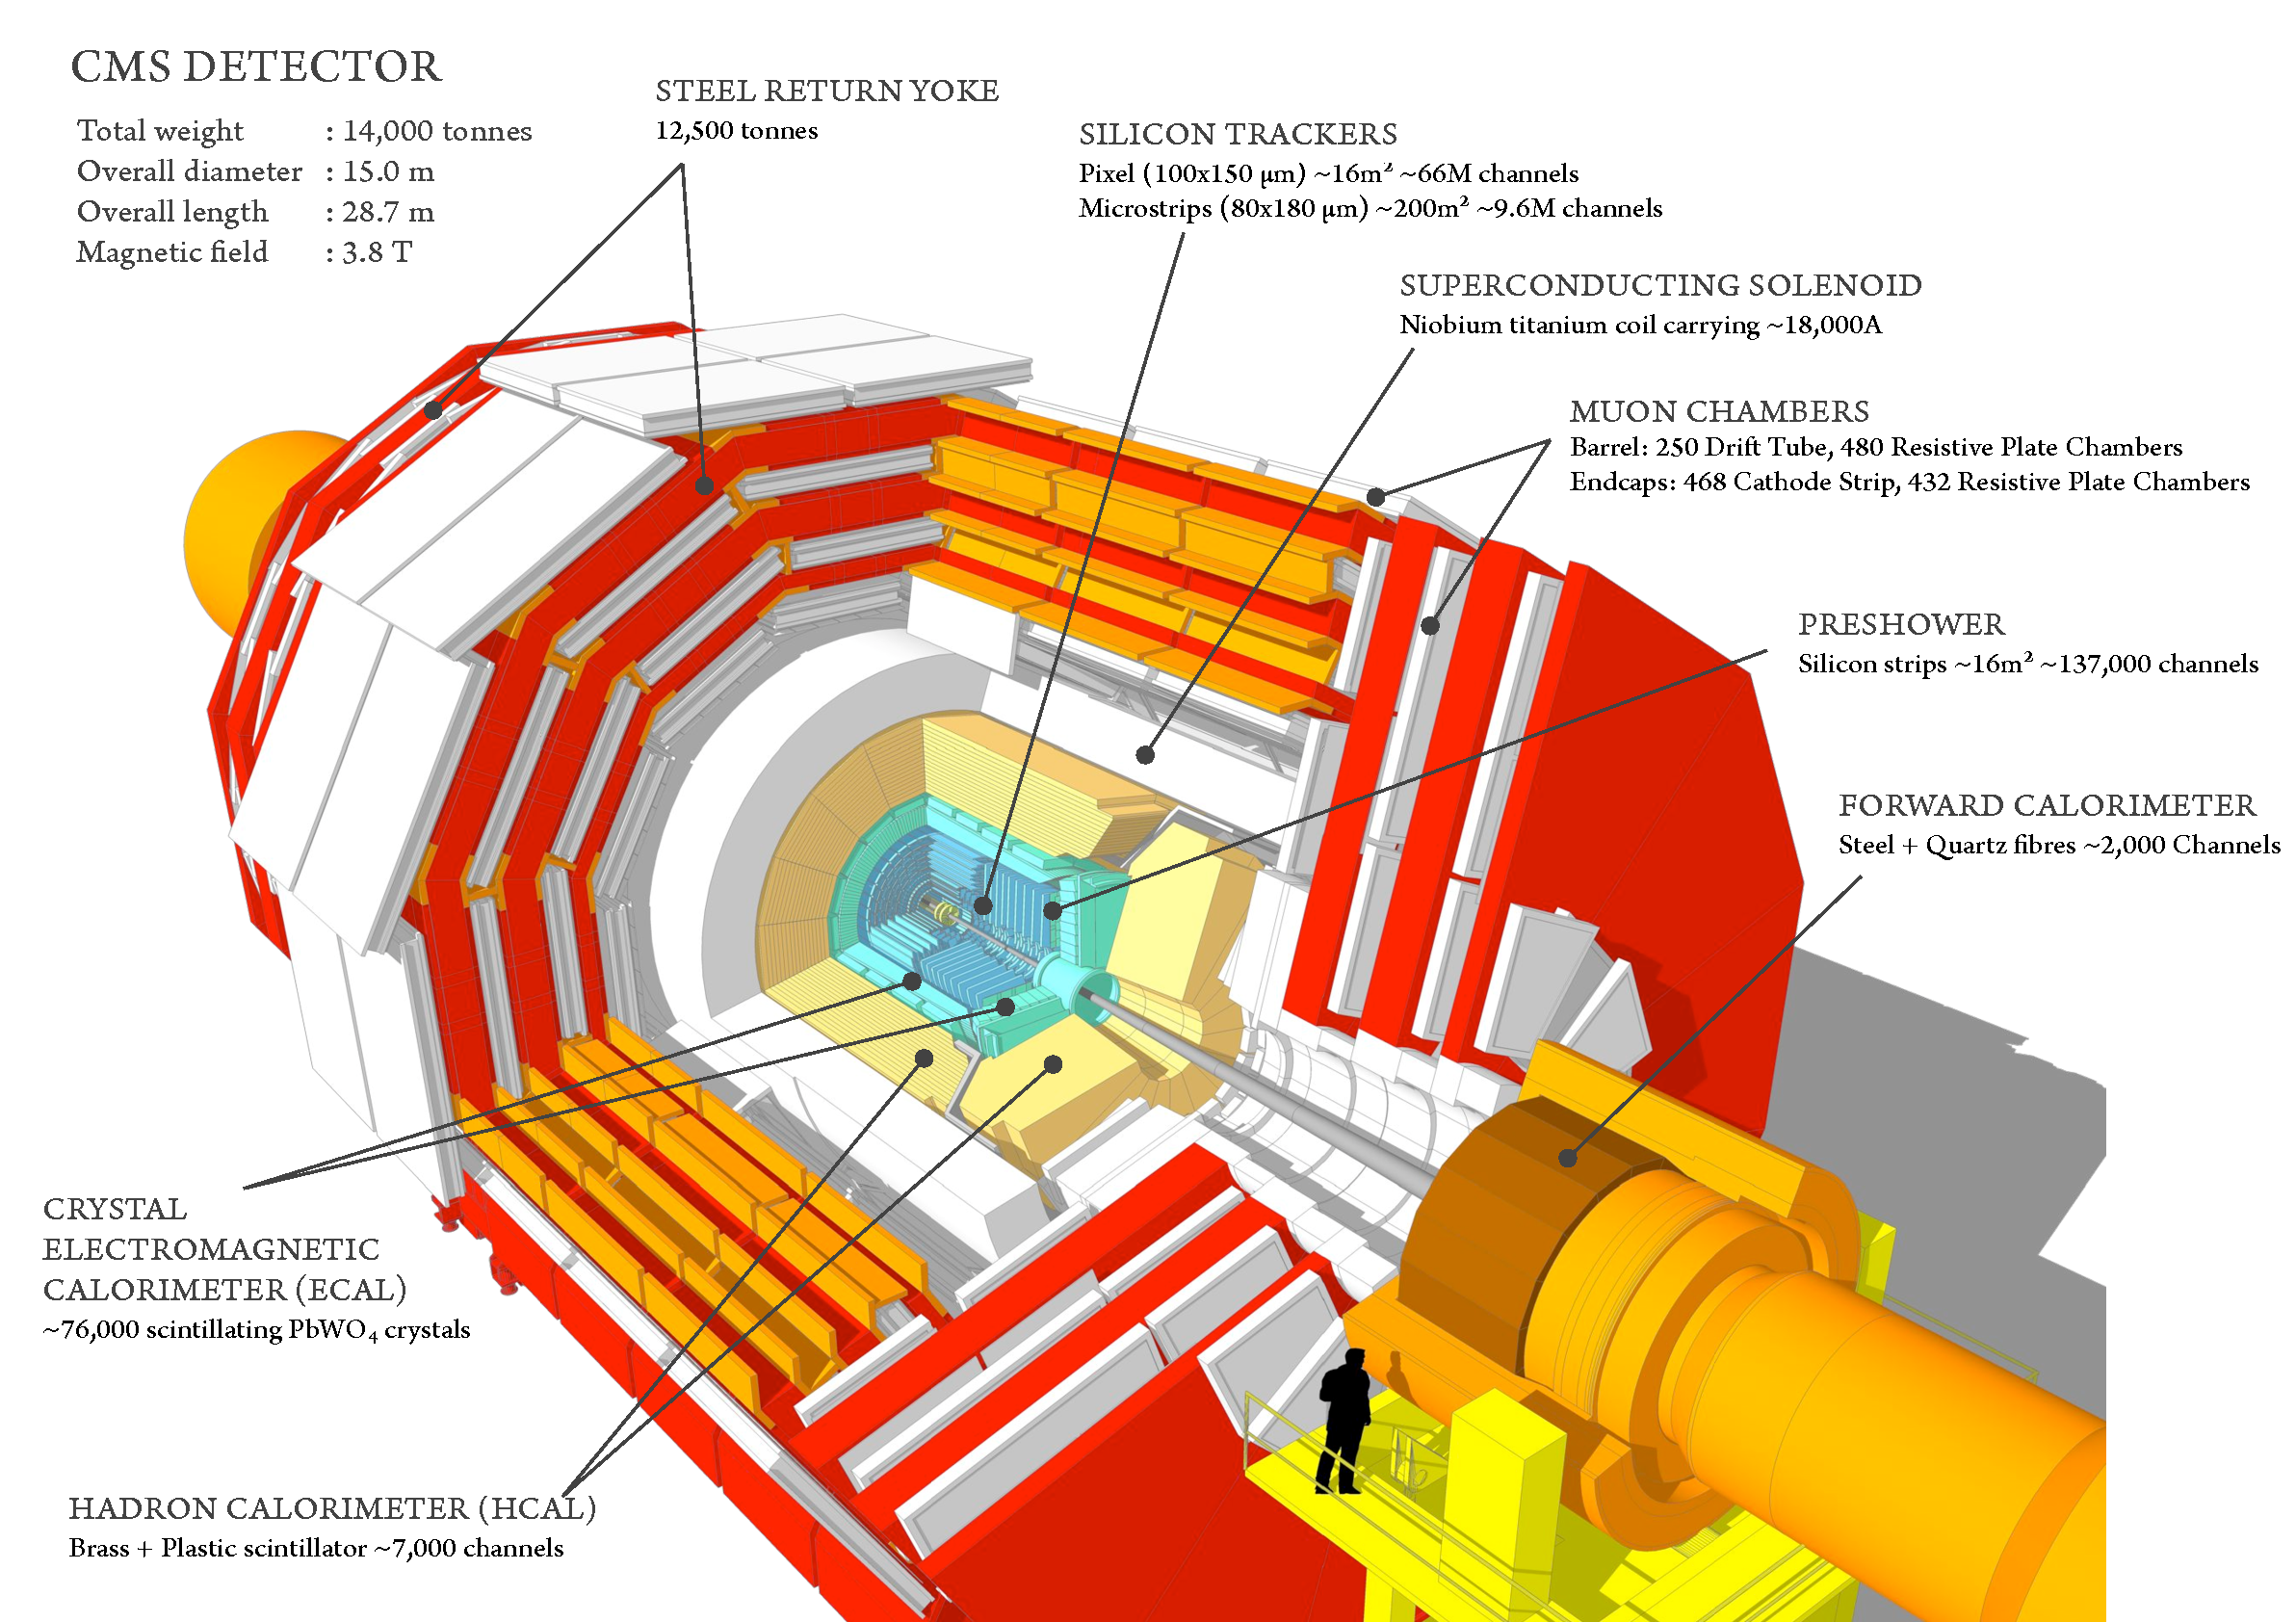
\includegraphics[width=5.5in]{images/cms_120918_03}
    \caption[Cutaway View of the CMS Detector]{A cutaway view of the CMS detector with its main subsystems and components labeled.\cite{CMScutaway}}
    \label{fig:CMScutaway}
\end{figure}

\begin{figure}[htbp]
  \centering
    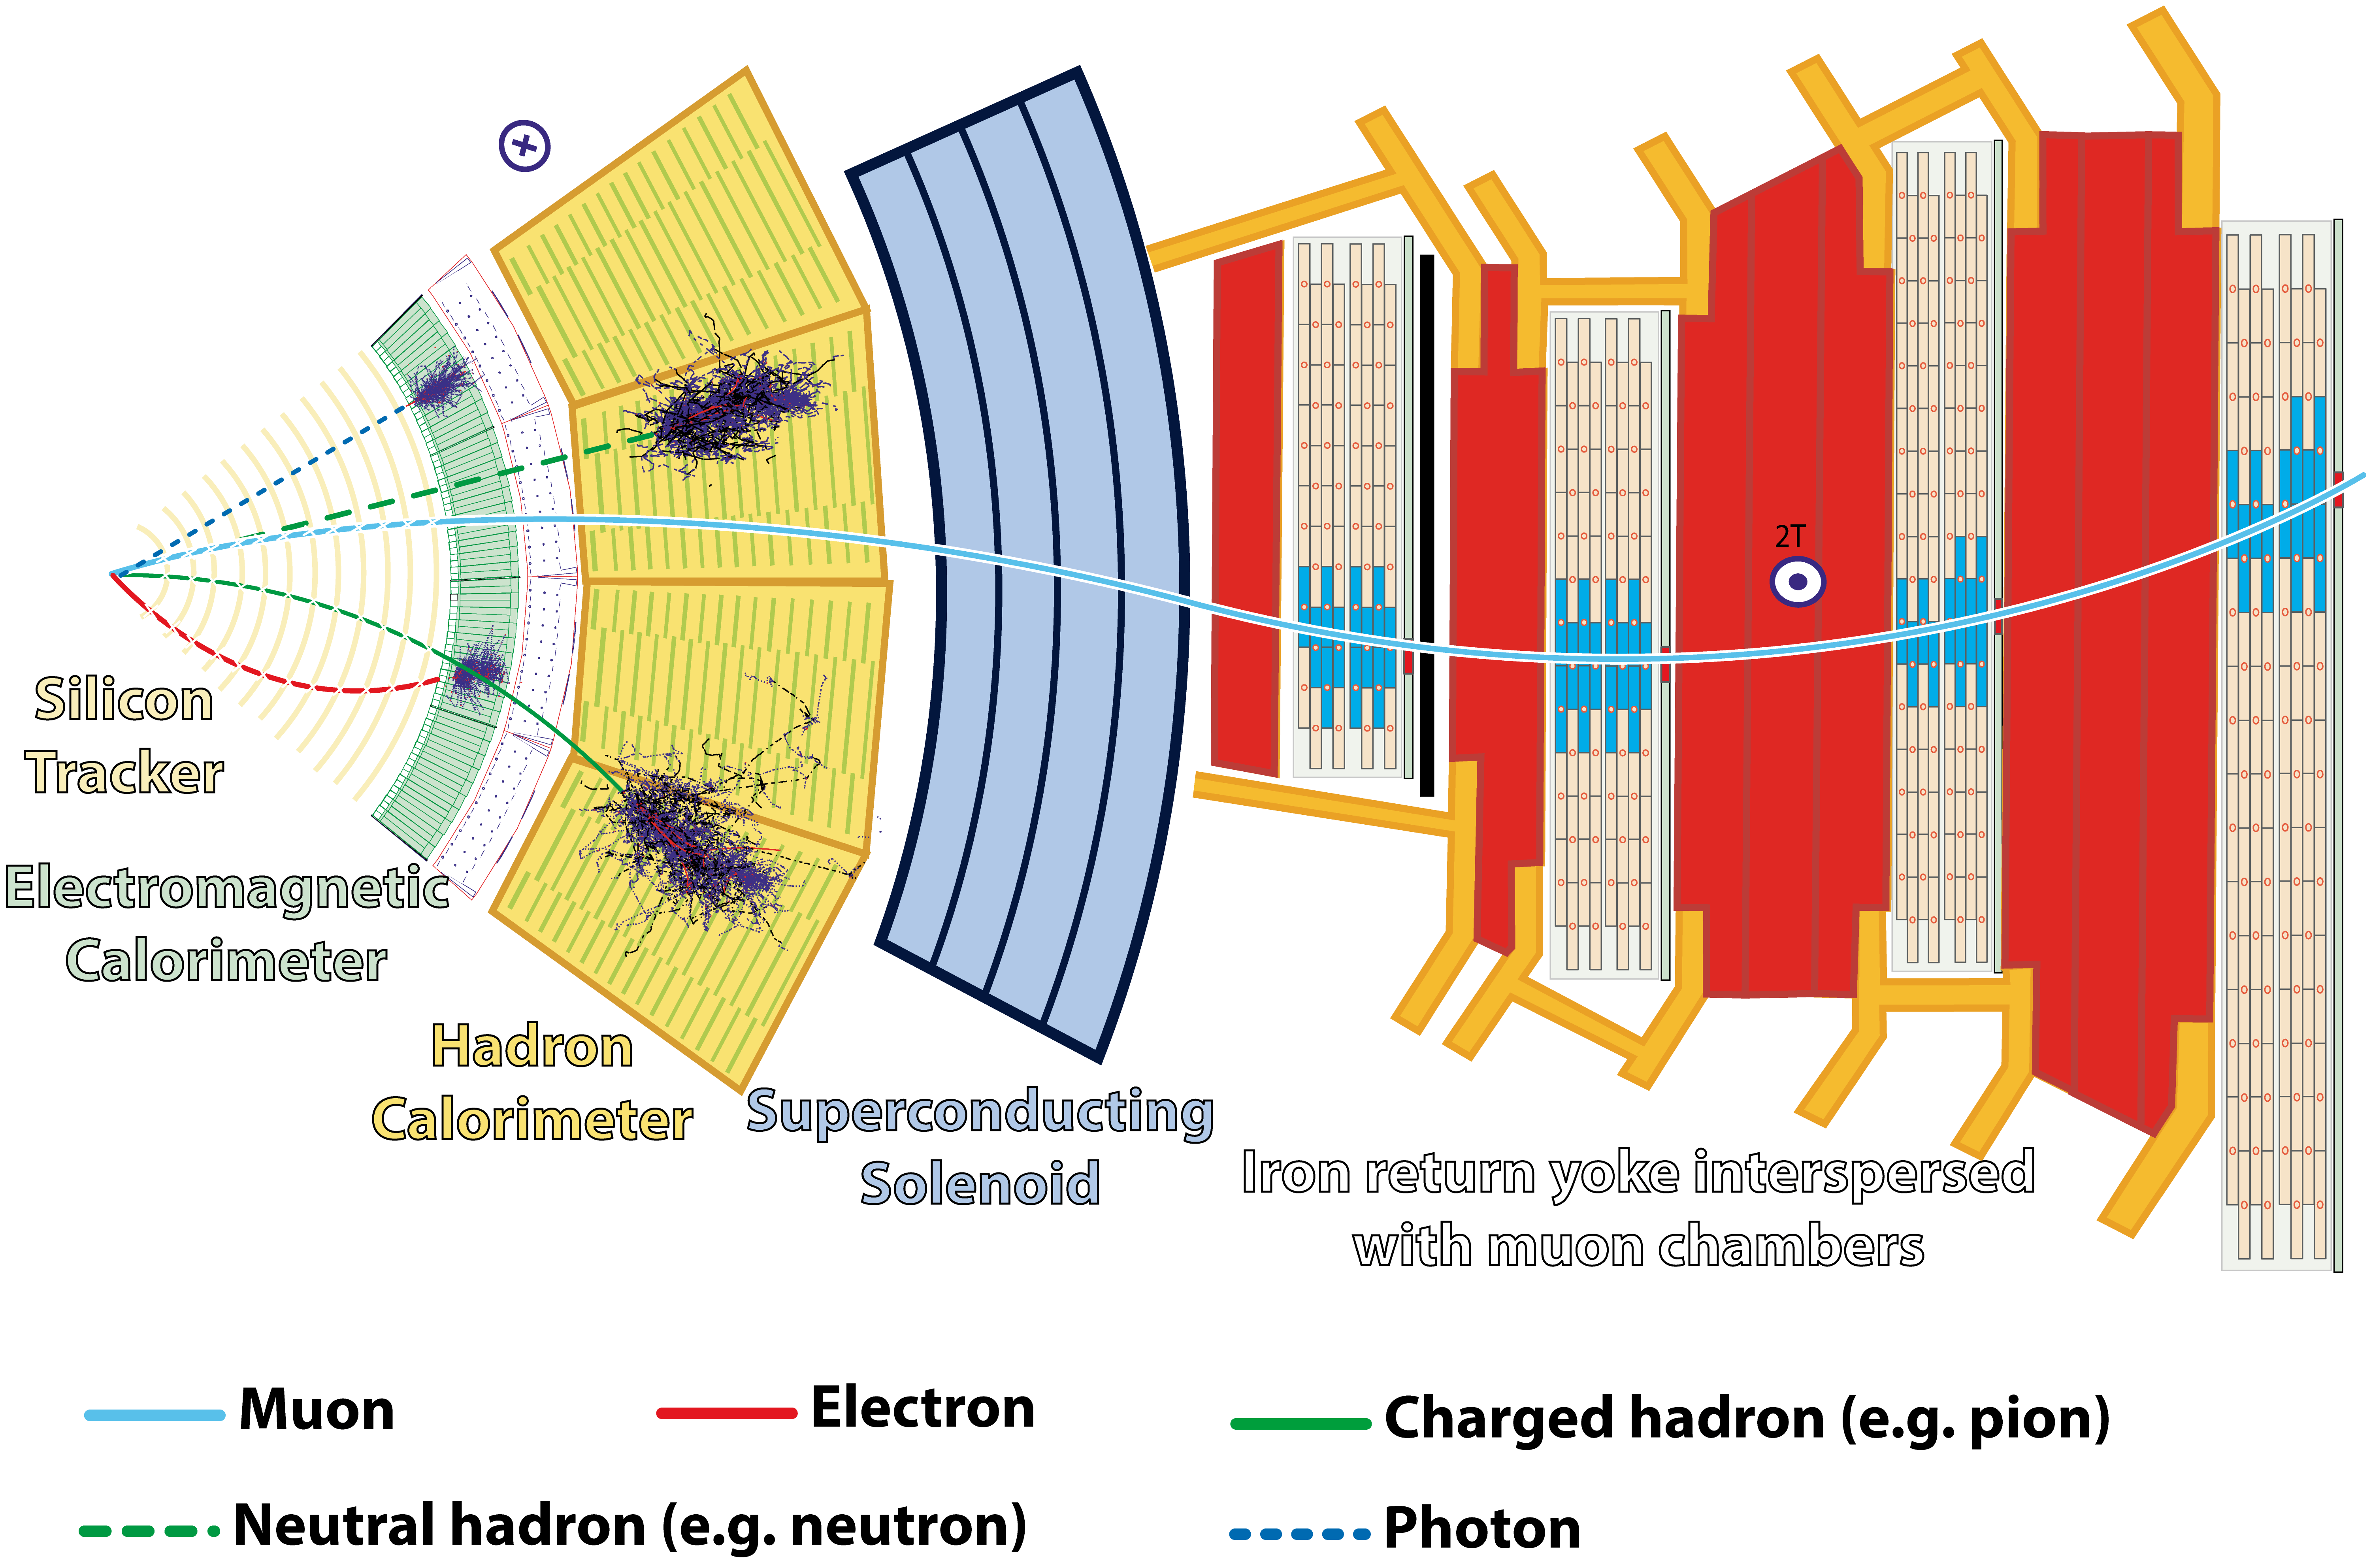
\includegraphics[width=5.5in]{images/CMSslice_whiteBackground}
    \caption[Cross Sectional View of the CMS Detector]{A cross sectional view of the CMS detector highlighting the different subsystems and the particles they are used to detect.\cite{CMSslice}}
    \label{fig:CMSslice}
\end{figure}

\subsection{Superconducting Solenoid}

\subsection{Silicon Tracker}

\subsection{Electromagnetic Calorimeter}

\subsection{Hadronic Calorimeter}

\subsection{The Muon System}

\subsection{Data Acquisition and Triggers}

\subsubsection{Level 1 trigger}

\subsubsection{High level trigger}

\subsection{Upgrades for Run 2}

%Many of the problems in theses and dissertations involve tables. The UF Graduate Counsel is very specific in the Table Requirements.\renewcommand*{\thefootnote}{\fnsymbol{footnote}}\footnote{an un-numbered footnote}\renewcommand*{\thefootnote}{\arabic{footnote}}\setcounter{footnote}{0}There should be no vertical lines in tables and only three horizontal lines. No bold text, etc., see the web site for the complete list of requirements.\footnote{and now we're back to normal footnote marking} One simple improvement can be incorporated by using tabularx instead of the tabular environment. This allows a table to be stretched the full text width easily, which avoids the centered or left aligned issue. \cite{garfinkle1991charged} Table \ref{first} is an examble of the tabularx code. Consectetur adipiscing elit. Fusce eget tempus lectus, non porttitor tellus. Aliquam molestie sed urna quis convallis. Aenean nibh eros, aliquam non eros in, tempus lacinia justo. In magna sapien, blandit a faucibus ac, scelerisque nec purus. 
% 
% \begin{table}[htbp]
%    \caption{A sample Table using tabularx}\label{first}
%    \begin{tabularx}{6.5in}{XXX}
%      \hline
%      First & Second & Third \\
%      \hline
%      12 & 45 & 26 \\
%      17 & 32 & 93 \\
%      text & 51 & can be there too. \\	
%      \epsfig{figure=images/cat.eps, scale=1} & 28 & Figures too - a cat. \\
%      \begin{turn}{0}\epsfig{figure=images/mouse.eps, scale=0.25}\end{turn} & 000 & and a mouse! \\
%      \hline
%    \end{tabularx}
%\end{table}
% 
% 
% Praesent fermentum felis nec massa interdum, vel dapibus mi luctus. Cras id fringilla mauris. Ut molestie eros mi, ut hendrerit nulla tempor et. Pellentesque tortor quam, mattis a scelerisque nec, euismod et odio. Mauris rhoncus metus sit amet risus mattis, eu mattis sem interdum.
%
% \begin{table}[htbp]
%    \caption{A sample Table using standard tablular}\label{first}
%    \begin{tabular}{c c c}
%      \hline
%      First & Second & Third \\
%      \hline
%      12 & 45 & 26 \\
%      17 & 32 & 93 \\
%      text & 51 & can be there too. \\	
%      \epsfig{figure=images/cat.eps, scale=1} & 28 & Figures too - a cat. \\
%      \begin{turn}{0}\epsfig{figure=images/mouse.eps, scale=0.25}\end{turn} & 000 & and a mouse! \\
%      \hline
%    \end{tabular}
%\end{table}
%
%\subsection{Platea Dictumst}
%Donec convallis scelerisque ante, in sollicitudin orci laoreet eu. Nam arcu magna, semper vel lorem eu, venenatis ultrices est. Nam aliquet ut erat ac scelerisque. Maecenas ut molestie mi. Phasellus ipsum magna, sollicitudin eu ipsum quis, imperdiet cursus turpis. Etiam pretium enim a fermentum accumsan. Morbi vel vehicula enim.
%
%
%\subsection{Long (and/or Wide) Tables}
%
%Another problem in LaTeX is the inability to handle long tables. While there are some packages that address this problem none of them quite fit the Editorial Office guidelines. The caption is not repeated but we do need "Table x-y. Continued" on each subsequent page and a repeat of the column headings on each page as well. The following table is the best example of the correct format I can produce. The disadvantage of this method is that much of it is manually set up and changes in the text will cause changes in the table. \citep{Moffatt69} For best results avoid the use of footnotemark and footnotetext commands inside of tables and try to keep your footnotes outside of floats whenever possible.
%
%
%
%\begin{table}
%\caption{Feasible triples for highly variable Grid, MLMMH.} \label{tbl1}
%\begin{tabularx}{6.5 in}{r l X}
%\hline {{Time (s)}} & {{Triple chosen}} & {{Other feasible triples}} \\ \hline
%0 & (1, 11, 13725) & (1, 12, 10980), (1, 13, 8235), (2, 2, 0), (3, 1, 0) \\
%2745 & (1, 12, 10980) & (1, 13, 8235), (2, 2, 0), (2, 3, 0), (3, 1, 0) \\
%5490 & (1, 12, 13725) & (2, 2, 2745), (2, 3, 0), (3, 1, 0) \\
%8235 & (1, 12, 16470) & (1, 13, 13725), (2, 2, 2745), (2, 3, 0), (3, 1, 0) \\
%10980 & (1, 12, 16470) & (1, 13, 13725), (2, 2, 2745), (2, 3, 0), (3, 1, 0) \\
%13725 & (1, 12, 16470) & (1, 13, 13725), (2, 2, 2745), (2, 3, 0), (3, 1, 0) \\
%16470 & (1, 13, 16470) & (2, 2, 2745), (2, 3, 0), (3, 1, 0) \\
%19215 & (1, 12, 16470) & (1, 13, 13725), (2, 2, 2745), (2, 3, 0), (3, 1, 0) \\
%21960 & (1, 12, 16470) & (1, 13, 13725), (2, 2, 2745), (2, 3, 0), (3, 1, 0) \\
%24705 & (1, 12, 16470) & (1, 13, 13725), (2, 2, 2745), (2, 3, 0), (3, 1, 0) \\
%27450 & (1, 12, 16470) & (1, 13, 13725), (2, 2, 2745), (2, 3, 0), (3, 1, 0) \\
%30195 & (2, 2, 2745) & (2, 3, 0), (3, 1, 0) \\
%32940 & (1, 13, 16470) & (2, 2, 2745), (2, 3, 0), (3, 1, 0) \\
%35685 & (1, 13, 13725) & (2, 2, 2745), (2, 3, 0), (3, 1, 0) \\
%38430 & (1, 13, 10980) & (2, 2, 2745), (2, 3, 0), (3, 1, 0) \\
%41175 & (1, 12, 13725) & (1, 13, 10980), (2, 2, 2745), (2, 3, 0), (3, 1, 0) \\
%43920 & (1, 13, 10980) & (2, 2, 2745), (2, 3, 0), (3, 1, 0) \\
%46665 & (2, 2, 2745) & (2, 3, 0), (3, 1, 0) \\
%49410 & (2, 2, 2745) & (2, 3, 0), (3, 1, 0) \\
%52155 & (1, 12, 16470) & (1, 13, 13725), (2, 2, 2745), (2, 3, 0), (3, 1, 0) \\
%54900 & (1, 13, 13725) & (2, 2, 2745), (2, 3, 0), (3, 1, 0) \\
%57645 & (1, 13, 13725) & (2, 2, 2745), (2, 3, 0), (3, 1, 0) \\
%60390 & (1, 12, 13725) & (2, 2, 2745), (2, 3, 0), (3, 1, 0) \\
%63135 & (1, 13, 16470) & (2, 2, 2745), (2, 3, 0), (3, 1, 0) \\
%65880 & (1, 13, 16470) & (2, 2, 2745), (2, 3, 0), (3, 1, 0) \\
%68625 & (2, 2, 2745) & (2, 3, 0), (3, 1, 0) \\
%71370 & (1, 13, 13725) & (2, 2, 2745), (2, 3, 0), (3, 1, 0) \\
%74115 & (1, 12, 13725) & (2, 2, 2745), (2, 3, 0), (3, 1, 0) \\
%76860 & (1, 13, 13725) & (2, 2, 2745), (2, 3, 0), (3, 1, 0) \\
%79605 & (1, 13, 13725) & (2, 2, 2745), (2, 3, 0), (3, 1, 0) \\
%82350 & (1, 12, 13725) & (2, 2, 2745), (2, 3, 0), (3, 1, 0) \\
%85095 & (1, 12, 13725) & (1, 13, 10980), (2, 2, 2745), (2, 3, 0), (3, 1, 0) \\
%87840 & (1, 13, 16470) & (2, 2, 2745), (2, 3, 0), (3, 1, 0) \\
%90585 & (1, 13, 16470) & (2, 2, 2745), (2, 3, 0), (3, 1, 0) \\
%93330 & (1, 13, 13725) & (2, 2, 2745), (2, 3, 0), (3, 1, 0) \\
%96075 & (1, 13, 16470) & (2, 2, 2745), (2, 3, 0), (3, 1, 0) \\
%98820 & (1, 13, 16470) & (2, 2, 2745), (2, 3, 0), (3, 1, 0) \\
%101565 & (1, 13, 13725) & (2, 2, 2745), (2, 3, 0), (3, 1, 0) \\
%104310 & (1, 13, 16470) & (2, 2, 2745), (2, 3, 0), (3, 1, 0) \\
%107055 & (1, 13, 13725) & (2, 2, 2745), (2, 3, 0), (3, 1, 0) \\
%109800 & (1, 13, 13725) & (2, 2, 2745), (2, 3, 0), (3, 1, 0) \\
%112545 & (1, 12, 16470) & (1, 13, 13725), (2, 2, 2745), (2, 3, 0), (3, 1, 0) \\
%\hline
%\end{tabularx}
%\end{table}
%
%\begin{table}[h!t!]
%\begin{tabularx}{6.5 in}{r l X}
%\multicolumn{3}{l}{Table \ref{tbl1}. Continued}\\%
%\hline {{Time (s)}} & {{Triple chosen}} & {{Other feasible triples}} \\ \hline
%115290 & (1, 13, 16470) & (2, 2, 2745), (2, 3, 0), (3, 1, 0) \\
%118035 & (1, 13, 13725) & (2, 2, 2745), (2, 3, 0), (3, 1, 0) \\
%120780 & (1, 13, 16470) & (2, 2, 2745), (2, 3, 0), (3, 1, 0) \\
%123525 & (1, 13, 13725) & (2, 2, 2745), (2, 3, 0), (3, 1, 0) \\
%126270 & (1, 12, 16470) & (1, 13, 13725), (2, 2, 2745), (2, 3, 0), (3, 1, 0) \\
%129015 & (2, 2, 2745) & (2, 3, 0), (3, 1, 0) \\
%131760 & (2, 2, 2745) & (2, 3, 0), (3, 1, 0) \\
%134505 & (1, 13, 16470) & (2, 2, 2745), (2, 3, 0), (3, 1, 0) \\
%137250 & (1, 13, 13725) & (2, 2, 2745), (2, 3, 0), (3, 1, 0) \\
%139995 & (2, 2, 2745) & (2, 3, 0), (3, 1, 0) \\
%142740 & (2, 2, 2745) & (2, 3, 0), (3, 1, 0) \\
%145485 & (1, 12, 16470) & (1, 13, 13725), (2, 2, 2745), (2, 3, 0), (3, 1, 0)\\%
%148230 & (2, 2, 2745) & (2, 3, 0), (3, 1, 0) \\
%150975 & (1, 13, 16470) & (2, 2, 2745), (2, 3, 0), (3, 1, 0) \\
%153720 & (1, 12, 13725) & (2, 2, 2745), (2, 3, 0), (3, 1, 0) \\
%156465 & (1, 13, 13725) & (2, 2, 2745), (2, 3, 0), (3, 1, 0) \\
%159210 & (1, 13, 13725) & (2, 2, 2745), (2, 3, 0), (3, 1, 0) \\
%161955 & (1, 13, 16470) & (2, 2, 2745), (2, 3, 0), (3, 1, 0) \\
%164700 & (1, 13, 13725) & (2, 2, 2745), (2, 3, 0), (3, 1, 0) \\
%\hline
%\end{tabularx}
%\end{table}
%
%\section{Ex id ullamcorper commodo}
%Augue sapien mattis leo, nec accumsan turpis quam at neque. Ut pellentesque velit sed placerat cursus. Integer congue urna non massa dictum, a pellentesque arcu accumsan. Nulla posuere, elit accumsan eleifend elementum, ipsum massa tristique metus, in ornare neque nisl sed odio. Nullam eget elementum nisi. Duis a consectetur erat, sit amet malesuada sapien. Aliquam nec sapien et leo sagittis porttitor at ut lacus. Vivamus vulputate elit vitae libero condimentum dictum. Nulla facilisi. Quisque non nibh et massa ullamcorper iaculis.
%
%Integer laoreet bibendum arcu non pulvinar. Curabitur ac magna nibh. Phasellus sed nisi semper, molestie neque at, tempus lacus. Aenean vitae lacinia est. Phasellus aliquam lacus sit amet placerat molestie. Sed sit amet bibendum lectus, ac ornare ligula. Curabitur porttitor interdum tortor a dignissim. Quisque a placerat nibh. Phasellus lobortis imperdiet augue, non congue est bibendum eu. Vivamus tincidunt quam eu fringilla laoreet.
%
%Maecenas efficitur dolor et ipsum convallis, ut fringilla neque luctus. Donec ac nisl quis leo gravida accumsan sit amet sed tellus. Quisque placerat hendrerit augue sit amet aliquet. Vestibulum laoreet consequat nunc, et egestas nisl auctor et. Duis scelerisque vulputate placerat. Proin tempus ligula ac tempor eleifend. Nullam est odio, commodo quis nisl eu, feugiat efficitur purus.
%
%Duis egestas in mauris vel efficitur. Sed a faucibus sem, non euismod enim. Maecenas nec nulla justo. Suspendisse ut orci ac mi aliquet tincidunt ac eget quam. Quisque ac mi sagittis, dapibus dui a, facilisis neque. Aenean euismod orci sem, non imperdiet ipsum pulvinar ac. Proin eu vestibulum magna, eu ullamcorper nulla. Etiam enim felis, dignissim eget commodo ac, faucibus nec justo. Nulla condimentum velit imperdiet ligula aliquam semper. Nulla facilisi. Ut in lobortis metus, at dictum ipsum. Suspendisse facilisis nec eros eget mollis. Vestibulum eget dolor ac mauris lobortis gravida. Suspendisse consectetur orci in risus pharetra, sed eleifend nisl lacinia. Mauris augue nibh, commodo sed sem at, congue molestie massa. Suspendisse sodales aliquet tellus, a tristique nunc aliquam id.


%\chapter{MATERIALS ANS METHODS} \label{materials}

\section{Consectetur Adipiscing Elit}

 Fusce eget tempus lectus, non porttitor tellus. Aliquam molestie sed urna quis convallis. Aenean nibh eros, aliquam non eros in, tempus lacinia justo. In magna sapien, blandit a faucibus ac, scelerisque nec purus. Praesent fermentum felis nec massa interdum, vel dapibus mi luctus. Cras id fringilla mauris. Ut molestie eros mi, ut hendrerit nulla tempor et. Pellentesque tortor quam, mattis a scelerisque nec, euismod et odio. Mauris rhoncus metus sit amet risus mattis, eu mattis sem interdum.

\subsection{This Is an Isolated Heading}
Either promote this to a section heading, add another subsection heading, or delete this heading.

\section{Augue sapien mattis leo}
Nec accumsan turpis quam at neque. Ut pellentesque velit sed placerat cursus. Integer congue urna non massa dictum, a pellentesque arcu accumsan. Nulla posuere, elit accumsan eleifend elementum, ipsum massa tristique metus, in ornare neque nisl sed odio. Nullam eget elementum nisi. Duis a consectetur erat, sit amet malesuada sapien. Aliquam nec sapien et leo sagittis porttitor at ut lacus. Vivamus vulputate elit vitae libero condimentum dictum. Nulla facilisi. Quisque non nibh et massa ullamcorper iaculis.


%\chapter{RESULTS} \label{results}

\section{Fusce Eget Tempus Lectus, }


\begin{equation}
A^2 + B^2 = C^2
\end{equation}

%\hline
\begin{algorithm}  {Euclid’s algorithm}
%\hline %
\singlespacing

\begin{algorithmic}[1]
%\caption{Euclid’s algorithm}\label{alg:euclid}
\Procedure{Euclid}{$a,b$}\Comment{The g.c.d. of a and b}
\State $r\gets a\bmod b$
\While{$r\not=0$}\Comment{We have the answer if r is 0}
\State $a\gets b$
\State $b\gets r$
\State $r\gets a\bmod b$
\EndWhile\label{euclidendwhile}
\State \textbf{return} $b$\Comment{The gcd is b}
\EndProcedure
%\hline
\end{algorithmic}
\end{algorithm}









\proposition{The Upsilon Function}

(1) If $\beta>0$ and $\alpha\neq0$, then for all $n\geq-1$,

$I_{n}(c;\alpha; \beta; \delta) = - \frac{e^{\alpha c}}{\alpha} \sum_{i=0}^{n}(\frac{\beta}{\alpha})^{n-i} Hh_{i}(\beta c -\delta)$

$$+ (\frac{\beta}{\alpha})^{n+1} \frac{\sqrt{2 \pi}}{\beta} e^{\frac{\alpha \delta}{\beta}+\frac{\alpha^{2}}{2\beta^{2}}} \phi(-\beta c + \delta + \frac{\alpha}{\beta})$$
(2) If $\beta<0$ and $\alpha<0$, then for all $x \geq -1$

$$I_{n}(c;\alpha; \beta; \delta) = - \frac{e^{\alpha c}}{\alpha} \sum_{i=0}^{n}(\frac{\beta}{\alpha})^{n-i} Hh_{i}(\beta c -\delta)$$

$$- (\frac{\beta}{\alpha})^{n+1} \frac{\sqrt{2 \pi}}{\beta} e^{\frac{\alpha \delta}{\beta}+\frac{\alpha^{2}}{2\beta^{2}}} \phi(\beta c - \delta - \frac{\alpha}{\beta})$$

\begin{proof}{Case 1.}

$\beta>0$ and $\alpha\neq0$. Since, for any constant $\alpha$ and $n \geq 0$, $e^{\alpha x} Hh_{n}(\beta x - \delta) \rightarrow 0$ as $x \rightarrow \infty$ thanks to (B4), integration by parts leads to

$$I_{n}=-\frac{1}{\alpha}Hh(\beta c -\delta) e^{\alpha c} + \frac{\beta}{\alpha}\int_{c}^{\infty} e^{\alpha x} Hh_{n-1}(\beta c - \delta)dx$$

In other words, we have a recursion, for $n \geq 0$, $I_{n}=-(e^{\alpha c}{\alpha})Hh_{n}(\beta c - \delta) + (\frac{\beta}{\alpha})I_{n-1}$ with

$$I_{-1}=\sqrt{2 \pi} \int_{c}{\infty}e^{\alpha x}\varphi(-\beta x +\delta)dx$$

$$=\frac{\sqrt{2 \pi}}{\beta} e^{\frac{\alpha \delta}{\beta}+\frac{\alpha^{2}}{2 \beta^{2}}}\phi(-\beta c + \delta +\frac{\alpha}{\beta})$$

Solving it yields, for $n \geq -1$,

$$I_{n}=-\frac{e^{\alpha c}}{\alpha}\sum_{i=0}^{n}(\frac{\beta}{\alpha})^{i}Hh_{n-i}(\beta c+\delta) + (\frac{\beta}{\alpha})^{n+1}I_{-1}$$

$$=-\frac{e^{\alpha c}}{\alpha}\sum_{i=0}^{n}(\frac{\beta}{\alpha})^{n-i} Hh_{i}(\beta c+\delta)$$

$$+ (\frac{\beta}{\alpha})^{n+1}\frac{\sqrt{2 \pi}}{\beta} e^{\frac{\alpha \delta}{\beta}+\frac{\alpha^{2}}{2 \beta^{2}}}\phi(-\beta c + \delta +\frac{\alpha}{\beta})$$

where the sum over an empty set is defined to be zero.
\end{proof}

\begin{proof}{Case2.} $\beta<0$ and $\alpha<0$. In this case, we must also have, for $n \geq 0$ and any constant $\alpha<0, e^{\alpha x}Hh_{n}(\beta x -\delta) \rightarrow 0$ as

$x \rightarrow \infty$, thanks to (B5). Using integration by parts, we again have the same recursion, for $n \geq 0, I_{n}=-(e^{\alpha c}/\alpha)Hh_{n}(\beta c - \delta)+(\beta / \alpha)I_{n-1}$, but with a different initial condition

$$I_{-1}=\sqrt{2 \pi}\int_{c}^{\infty}e^{\alpha x}\varphi(-\beta x + \delta)dx$$

$$=-\frac{\sqrt{2 \pi}}{\beta} exp\{\frac{\alpha \delta}{\beta}+\frac{\alpha^{2}}{2 \beta^{2}}\}\phi(\beta c - \delta -\frac{\alpha}{\beta})$$

Solving it yields (B8), for $n \geq -1$.

\end{proof}

Finally, we sum the double exponential and the normal random variables

Proposition B.3.

Suppose $\{\xi_{1},\xi_{2},...\}$ is a sequence of i.i.d. exponential random variables with rate $\eta>0$, and Z is a normal variable with distribution $N(0,\sigma^{2})$. Then for every $ n \geq 1$, we have: (1) The density functions are given by:

$$f_{Z+\sum_{i=1}^{n}\xi_{i}}(t)=(\sigma\eta)^{n}\frac{e^{(\sigma\eta)^{2}/2}}{\sigma\sqrt{2\pi}}e^{-t\eta}Hh_{n-1}(-\frac{t}{\sigma}+\sigma\eta)$$

$$f_{Z-\sum_{i=1}^{n}\xi_{i}}(t)=(\sigma\eta)^{n}\frac{e^{(\sigma\eta)^{2}/2}}{\sigma\sqrt{2\pi}}e^{-t\eta}Hh_{n-1}(\frac{t}{\sigma}+\sigma\eta)$$
(2) The tail probabilities are given by

$$P(Z+\sum_{i=1}^{n}\xi_{i}\geq x) = (\sigma\eta)^{n}\frac{e^{(\sigma\eta)^{2}/2}}{\sigma\sqrt{2\pi}}e^{-t\eta}I_{n-1}(x;-\eta,-\frac{1}{\sigma},-\sigma\eta)$$

$$P(Z-\sum_{i=1}^{n}\xi_{i}\geq x) = (\sigma\eta)^{n}\frac{e^{(\sigma\eta)^{2}/2}}{\sigma\sqrt{2\pi}}e^{-t\eta}I_{n-1}(x;\eta,\frac{1}{\sigma},-\sigma\eta)$$

Proof. Case 1. The densities of $Z+\sum_{i=1}^{n}\xi_{i}$, and $Z-\sum_{i=1}^{n}\xi_{i}$. We have

$$f_{Z+\sum_{i=1}^{n}\xi_{i}}(t)=\int_{-\infty}^{\infty}f_{\sum_{i=1}^{n}\xi_{i}}(t-x)f_{Z}(x)dx$$

$$=e^{-t\eta}(\eta^{n})\int_{-\infty}{t}\frac{e^{x\eta}(t-x)^{n-1}}{(n-1)!}\frac{1}{\sigma\sqrt{2\pi}}e^{-x^{2}/(2\sigma^{2})}dx$$

$$=e^{-t\eta}(\eta^{n})e^{(\sigma\eta)^{2}/(2)}\int_{-\infty}{t}\frac{(t-x)^{n-1}}{(n-1)!}\frac{1}{\sigma\sqrt{2\pi}}e^{-(x-\sigma^{2}\eta)^{2}/(2\sigma^{2})}dx$$

Letting $y=(x-\sigma^{2}\eta)/\sigma$ yields

$$f_{Z+\sum_{i=1}^{n}\xi_{i}}(t)=e^{-t\eta}(\eta^{n})e^{(\sigma\eta)^{2}/(2)}\sigma^{n-1}$$

$$\times\int_{-\infty}^{t/\sigma-\sigma\eta}\frac{(t/\sigma - y -\sigma\eta)^{n-1}}{(n-1)!}\frac{1}{\sqrt{2\pi}}e^{-y^{2}/2}dy$$

$$=\frac{e^{(\sigma\eta)^{2}/2}}{\sqrt{2\pi}}(\sigma^{n-1}\eta^{n})e^{-t\eta}Hh_{n-1}(-t/\sigma + \sigma\eta)$$

because $(1/(n-1)!)\int_{-\infty}{a}(a-y)^{n-1}e^{-y^{2}/2}dy=Hh_{n-1}(a)$. The derivation of $f_{Z+\sum_{i=1}^{n}\xi_{i}}(t)$ is similar.

Case 2. $P(Z+\sum_{i=1}^{n}\xi_{i}\geq x)$ and $P(Z-\sum_{i=1}^{n}\xi_{i}\geq x)$. From (B9), it is clear that

$$P(Z+\sum_{i=1}^{n}\xi_{i}\geq x)=\frac{(\sigma\eta)^{n}e^{(\sigma\eta)^{2}/2}}{\sigma\sqrt{2\pi}}\int_{x}^{\infty}e^{(-i\eta)}Hh_{n-1}(-\frac{t}{\sigma}+\sigma\eta)dt$$

$$=\frac{(\sigma\eta)^{n}e^{(\sigma\eta)^{2}/2}}{\sigma\sqrt{2\pi}}I_{n-1}(x;-\eta,-\frac{1}{\sigma},-\sigma\eta)dt$$

by (B6). We can compute
$P(Z-\sum_{i=1}^{n}\xi_{i}\geq x)$ similarly.

\theorem{Theorem} With $\pi_{n}:= P(N(t)=n)=e^{-\lambda T}(\lambda T)^{n}/n!$ and $I_{n}$ in Proposition \ref{first}.
, we have

$$P(Z(T)\geq a)=\frac{e^{(\sigma \eta_{1})^{2} T/2}}{\sigma \sqrt{2 \pi T}} \sum_{n=1}^{\infty} \pi_{n} \sum_{k=1}^{n} P_{n,k}(\sigma\sqrt{T}\eta_{1})^{k}\times I_{k-1}(a-\mu T; -\eta_{1},-\frac{1}{\sigma\sqrt{T}},-\sigma\eta_{1}\sqrt{T})$$

$$+\frac{e^{(\sigma\eta_{2})^{2}T/2}}{\sigma\sqrt{2\pi T}}\sum_{n=1}^{\infty}\pi_{n}\sum_{k=1}^{n}Q_{n,k}(\sigma\sqrt{T}\eta_{2})^{k}$$

$$\times I_{k-1}(a-\mu T; \eta_{2},\frac{1}{\sigma\sqrt{T}},-\sigma\eta_{2}\sqrt{T})$$

$$+\pi_{0}\phi(-\frac{a-\mu T}{\sigma\sqrt{T}})$$

Proof by the decomposition (B2)

$$P(Z(T) \geq a)= \sum_{n=0}^{\infty}\pi_{n} P(\mu T +\sigma\sqrt{T} Z + \sum_{j=1}^{n}Y_{j} \geq a)$$

$$=\pi_{0}P(\mu T +\sigma\sqrt{T} Z  \geq a)$$

$$+\sum_{n=1}^{\infty}\pi_{n}\sum_{k=1}^{n}P_{n,k} P(\mu T +\sigma\sqrt{T} Z + \sum_{j=1}^{n}\xi_{j}^{+} \geq a)$$

$$+\sum_{n=1}^{\infty}\pi_{n}\sum_{k=1}^{n}Q_{n,k} P(\mu T +\sigma\sqrt{T} Z - \sum_{j=1}^{n}\xi_{j}^{-} \geq a)$$

The result now follows via (B11) and (B12) for $\eta_{1} > 1$ and $\eta_{2} >0$. 
\chapter{ANALYSIS STRATEGY} \label{strategy}

The first \VHbb\ analysis conducted by the CMS collaboration in 2012\cite{HIG13012} demonstrated that an observation of the \Hbb\ decay was feasible by combining searches for the \ZnnHbb, \WenHbb, \WmnHbb, \ZeeHbb, and \ZmmHbb\ decay channels. The overall strategy that it pioneered has remained largely intact, even through the transition to LHC Run 2. The search for \VHbb\ using the 2016 dataset would establish evidence for the \Hbb\ decay in 2017\cite{CMSVHbbEvidence} with only incremental improvements. The search for \VHbb\ using the 2017 dataset would build on the physics insights and experiences obtained the year prior while bringing to bear additional event reconstruction techniques and deep learning to finally observe the \Hbb\ decay in 2018.\cite{HIG18016} This chapter describes the analysis strategy used by CMS to achieve its state of the art result, with a focus on the \ZnnHbb\ decay channel in particular.\footnote{This chapter includes content adapted from Ref. \cite{CMSVHbbEvidence} and \cite{HIG18016}, as the author's work directly contributed to those publications.}

\section{Data and Simulation}

\subsection{Data}

The datasets used for this analysis were collected by the CMS detector throughout 2017 and produced by proton-proton collisions with a center-of-mass energy $\sqrt{s} = 13\ \TeV$ and a bunch spacing of 25 ns. The \ZnnH\ channel uses the MET dataset, the \WenH\ channel uses the SingleElectron dataset, the \WmnH\ channel uses the SingleMuon dataset, the \ZeeH\ channel uses the DoubleEG dataset, and the \ZmmH\ channel uses the DoubleMuon dataset. All of these primary datasets have an approximate total luminosity of 41.3 \invfb\ when only considering \textit{golden} events, which were certified by data quality monitoring teams to have been collected during periods of normal function for all detector subsystems. The JSON certification file \texttt{Cert\_294927-306462\_13TeV\_EOY2017ReReco\_Collisions17\_JSON\_v1.txt} was used to filter for golden events.

\subsection{Simulation}

Simulated samples for each of the relevant signal and background processes are used to design and validate the analysis strategy in an unbiased manner. These samples are produced using different Monte-Carlo (MC) generators and processed by the \textsc{\small GEANT4}\cite{GEANT4A,GEANT4B,GEANT4C} software which realistically models the detector's response to the passage of particles through its materials. The reconstruction of these MC events was performed using CMS SoftWare (CMSSW) version 94X releases set to match the 2017 data taking conditions.

The signal samples, generated using the \textsc{\small POWHEG} v2\cite{POWHEGA,POWHEGB,POWHEGC} event generator, are listed in Table \ref{tbl:MCsignal}. The quark-induced signal processes are generated to next-to-leading order (NLO) accuracy in QCD using the MiNLO procedure \cite{MINLOA,MINLOB}, while the gluon-induced contributions to the $ZH$ signal processes are generated only to leading order (LO) accuracy in QCD. Their production cross sections and branching fractions are taken to be the state of the art values calculated for a Higgs boson mass of $\massH = 125\ \GeV$ from Ref. \cite{CERNYR4}, and specifically those listed in sections \ref{productionmodes} and \ref{decaymodes}. These production cross sections are further rescaled to next-to-next-to-leading order (NNLO) accuracy in QCD and NLO electroweak accuracy as a function of the transverse momentum of the vector boson \pTV, according to the combined calculations of the \textsc{\small VHNNLO}\cite{VHNNLOA,VHNNLOB,VHNNLOC,VHNNLOD}, \textsc{\small VH@NNLO}\cite{VHATNNLOA,VHATNNLOB}, and \textsc{\small HAWK} v2.0\cite{HAWK} event generators as described in Ref. \cite{CERNYR4}. The event weights used to rescale the samples are specific to each signal process and an example of the weights applied to the $\bosWp(\ell\nu)\Htobb$ channel are shown in Figure \ref{fig:VHNNLOweight}.

\begin{table}[htbp]
  \caption[Signal Samples for \VHbb\ 2017]{The Monte-Carlo samples and their cross sections for the signal processes considered by the 2017 \VHbb\ analysis.}
  \label{tbl:MCsignal}
  \small
  \begin{tabularx}{6.5in}{lX}
    \hline
    Sample                                                        & $\sigma (\pb)$                                   \\
    \hline
    \texttt{WminusH\_HToBB\_WToLNu\_M125\_13TeV\_powheg\_pythia8} & $0.5824 \times 0.533 \times 0.108535$            \\
    \texttt{WplusH\_HToBB\_WToLNu\_M125\_13TeV\_powheg\_pythia8}  & $0.5824 \times 0.840 \times 0.108535$            \\
    \texttt{ZH\_HToBB\_ZToLL\_M125\_13TeV\_powheg\_pythia8}       & $0.5824 \times (0.8839 - 0.1227) \times 0.10974$ \\
    \texttt{ZH\_HToBB\_ZToNuNu\_M125\_13TeV\_powheg\_pythia8}     & $0.5824 \times (0.8839 - 0.1227) \times 0.20103$ \\
    \texttt{ggZH\_HToBB\_ZToLL\_M125\_13TeV\_powheg\_pythia8}     & $0.5824 \times 0.1227 \times 0.10974$            \\
    \texttt{ggZH\_HToBB\_ZToNuNu\_M125\_13TeV\_powheg\_pythia8}   & $0.5824 \times 0.1227 \times 0.20103$            \\
    \hline
  \end{tabularx}
\end{table}

\begin{figure}[htbp]
  \centering
    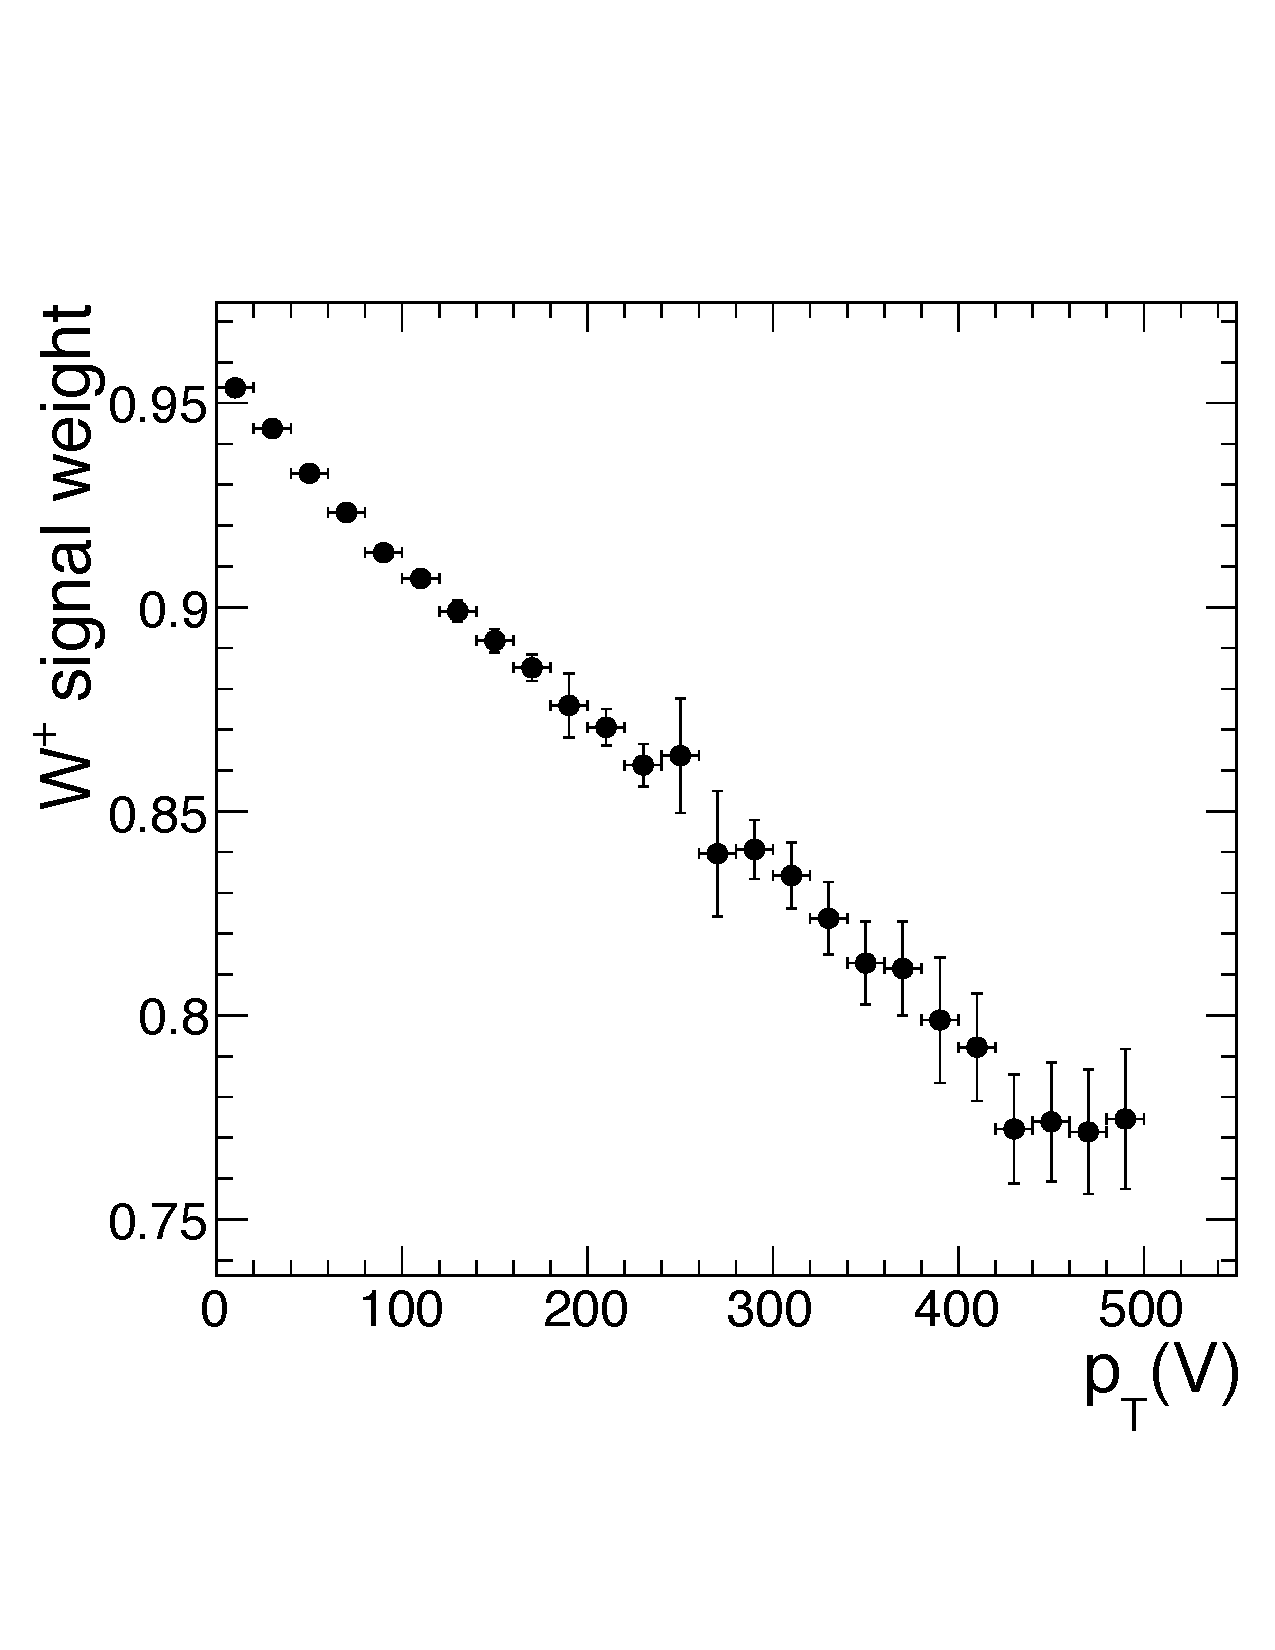
\includegraphics[width=3in]{images/ewk_wplush_correction}
    \caption[2017 Signal MC Rescaling Weights for $\bosWp(\ell\nu)\Htobb$]{The event weights used to rescale the production cross section of the $\bosWp(\ell\nu)\Htobb$ signal Monte-Carlo sample to NNLO QCD and NLO electroweak accuracy.}
    \label{fig:VHNNLOweight}
\end{figure}

The diboson samples listed in Table \ref{tbl:MCdiboson} are generated using the \textsc{\small MadGraph5\_amc@NLO} v2.4.2\cite{AMCNLO} event generator at NLO accuracy with the FxFx\cite{FXFX} merging scheme and up to two additional partons. The exception is the inclusive \bosZ\bosZ\ sample which is only simulated to LO accuracy and generated using \textsc{\small PYTHIA} v8.230\cite{PYTHIA8} event generator. Although the cross section of the \texttt{ZZTo2L2Q} sample has been obtained from an NLO calculation, the other cross sections are taken to be the product of their measured inclusive cross sections\cite{WWxsec,WZxsec,ZZxsec} and the appropriate branching ratio as computed by the Particle Data Group (PDG) in Ref. \cite{PDG2018}.

\begin{table}[htbp]
  \caption[Diboson Samples for \VHbb\ 2017]{The Monte-Carlo samples and their cross sections for the diboson processes considered by the 2017 \VHbb\ analysis.}
  \label{tbl:MCdiboson}
  \begin{tabularx}{6.5in}{lX}
    \hline
    Sample                                                      & $\sigma (\pb)$ \\
    \hline
    \texttt{WWTo1L1Nu2Q\_13TeV\_amcatnloFXFX\_madspin\_pythia8} & 50.86          \\
    \texttt{WZTo1L1Nu2Q\_13TeV\_amcatnloFXFX\_madspin\_pythia8} & 10.88          \\
    \texttt{ZZ\_TuneCP5\_13TeV-pythia8}                         & 14.60          \\
    \texttt{ZZTo2L2Q\_13TeV\_amcatnloFXFX\_madspin\_pythia8}    & 3.69           \\
    \hline
  \end{tabularx}
\end{table}

The \bosV+jets samples are also produced using the \textsc{\small MadGraph5\_amc@NLO} v2.4.2 event generator but at LO accuracy with the MLM matching scheme\cite{MLM}. Besides their inclusive and HT-binned configurations, \qrkb-quark enriched versions with up to four additional partons are also generated to increase the statistical power of these samples in the phase space most relevant for signal events because the \bosV+jets processes are the primary irreducible backgrounds. The samples for \bosW+jets with $\bosW \rightarrow \ell\nu$ are listed in Table \ref{tbl:MCWtoLNu}, while the samples for \bosZ+jets with $\bosZ \rightarrow \ell\bar{\ell}$ are listed in Table \ref{tbl:MCZtoLL} and with $\bosZ \rightarrow \nu\bar{\nu}$ are listed in Table \ref{tbl:MCZtoNuNu}. The cross sections of the \bosV+jets samples are multiplied by \textit{k}-factors of 1.21 and 1.23 for the \bosW+jets and \bosZ+jets samples, respectively, which rescale them to their NNLO cross sections as calculated by the \textsc{\small FEWZ} 3.1\cite{FEWZA,FEWZB,FEWZC} software. The cross sections of the \qrkb-quark enriched samples are further multiplied by a stitching factor which allows them to be used in conjunction with the inclusive and HT-binned versions by appropriately scaling their cross sections.

\begin{table}[htbp]
  \caption[\bosW+jets $(\bosW \rightarrow \ell\bar{\nu})$ Samples for \VHbb\ 2017]{The Monte-Carlo samples and their cross sections for the \bosW+jets $(\bosW \rightarrow \ell\bar{\nu})$ processes considered by the 2017 \VHbb\ analysis. Stitching factors of 1.5 and 1.12 are applied to the \texttt{WBJets} and \texttt{BGenFilter} \qrkb-quark enriched samples, respectively.}
  \label{tbl:MCWtoLNu}
  \small
  \begin{tabularx}{6.5in}{lX}
    \hline
    Sample                                                                 & $\sigma (\pb)$                 \\
    \hline
    \texttt{WJetsToLNu\_TuneCP5\_13TeV-madgraphMLM-pythia8}                & $1.21 \times 52940.0$          \\
    \texttt{WJetsToLNu\_HT-100To200\_TuneCP5\_13TeV-madgraphMLM-pythia8}   & $1.21 \times 1395.0$           \\
    \texttt{WJetsToLNu\_HT-200To400\_TuneCP5\_13TeV-madgraphMLM-pythia8}   & $1.21 \times 407.9$            \\
    \texttt{WJetsToLNu\_HT-400To600\_TuneCP5\_13TeV-madgraphMLM-pythia8}   & $1.21 \times 57.48$            \\
    \texttt{WJetsToLNu\_HT-600To800\_TuneCP5\_13TeV-madgraphMLM-pythia8}   & $1.21 \times 12.87$            \\
    \texttt{WJetsToLNu\_HT-800To1200\_TuneCP5\_13TeV-madgraphMLM-pythia8}  & $1.21 \times 5.366$            \\
    \texttt{WJetsToLNu\_HT-1200To2500\_TuneCP5\_13TeV-madgraphMLM-pythia8} & $1.21 \times 1.074$            \\
    \texttt{WJetsToLNu\_HT-2500ToInf\_TuneCP5\_13TeV-madgraphMLM-pythia8}  & $1.21 \times 0.03216$          \\
    \texttt{WBJetsToLNu\_Wpt-100to200\_TuneCP5\_13TeV-madgraphMLM-pythia8} & $1.21 \times 1.5 \times 7.35$  \\
    \texttt{WBJetsToLNu\_Wpt-200toInf\_TuneCP5\_13TeV-madgraphMLM-pythia8} & $1.21 \times 1.5 \times 1.1$   \\
    \texttt{WJetsToLNu\_BGenFilter\_Wpt-100to200\_TuneCP5\_13TeV}          & $1.21 \times 1.12 \times 26.6$ \\
    \texttt{  -madgraphMLM-pythia8}                                        &                                \\
    \texttt{WJetsToLNu\_BGenFilter\_Wpt-200toInf\_TuneCP5\_13TeV}          & $1.21 \times 1.12 \times 3.9$  \\
    \texttt{  -madgraphMLM-pythia8}                                        &                                \\
    \hline
  \end{tabularx}
\end{table}

\begin{table}[htbp]
  \caption[\bosZ+jets $(\bosZ \rightarrow \ell\bar{\ell})$ Samples for \VHbb\ 2017]{The Monte-Carlo samples and their cross sections for the \bosZ+jets $(\bosZ \rightarrow \ell\bar{\ell})$ processes considered by the 2017 \VHbb\ analysis. Stitching factors of 1.085 and 1.15 are applied to the \texttt{DYBJetsToLL} and \texttt{BGenFilter} \qrkb-quark enriched samples, respectively.}
  \label{tbl:MCZtoLL}
  \small
  \begin{tabularx}{6.5in}{lX}
    \hline
    Sample                                                              & $\sigma (\pb)$                    \\
    \hline
    \texttt{DYJetsToLL\_M-4to50\_HT-100to200\_TuneCP5\_13TeV}           & $1.23 \times 204.0$               \\
    \texttt{  -madgraphMLM-pythia8}                                     &                                   \\
    \texttt{DYJetsToLL\_M-4to50\_HT-200to400\_TuneCP5\_13TeV}           & $1.23 \times 54.4$                \\
    \texttt{  -madgraphMLM-pythia8}                                     &                                   \\
    \texttt{DYJetsToLL\_M-4to50\_HT-400to600\_TuneCP5\_13TeV}           & $1.23 \times 5.70$                \\
    \texttt{  -madgraphMLM-pythia8}                                     &                                   \\
    \texttt{DYJetsToLL\_M-4to50\_HT-600toInf\_TuneCP5\_13TeV}           & $1.23 \times 1.85$                \\
    \texttt{  -madgraphMLM-pythia8}                                     &                                   \\
    \texttt{DYJetsToLL\_M-50\_TuneCP5\_13TeV}                           & $1.23 \times 5343.0$              \\
    \texttt{  -madgraphMLM-pythia8}                                     &                                   \\
    \texttt{DYJetsToLL\_M-50\_HT-100to200\_TuneCP5\_13TeV}              & $1.23 \times 161.1$               \\
    \texttt{  -madgraphMLM-pythia8}                                     &                                   \\
    \texttt{DYJetsToLL\_M-50\_HT-200to400\_TuneCP5\_13TeV}              & $1.23 \times 48.66$               \\
    \texttt{  -madgraphMLM-pythia8}                                     &                                   \\
    \texttt{DYJetsToLL\_M-50\_HT-400to600\_TuneCP5\_13TeV}              & $1.23 \times 6.97$                \\
    \texttt{  -madgraphMLM-pythia8}                                     &                                   \\
    \texttt{DYJetsToLL\_M-50\_HT-600to800\_TuneCP5\_13TeV}              & $1.23 \times 1.743$               \\
    \texttt{  -madgraphMLM-pythia8}                                     &                                   \\
    \texttt{DYJetsToLL\_M-50\_HT-800to1200\_TuneCP5\_13TeV}             & $1.23 \times 0.805$               \\
    \texttt{  -madgraphMLM-pythia8}                                     &                                   \\
    \texttt{DYJetsToLL\_M-50\_HT-1200to2500\_TuneCP5\_13TeV}            & $1.23 \times 0.193$               \\
    \texttt{  -madgraphMLM-pythia8}                                     &                                   \\
    \texttt{DYJetsToLL\_M-50\_HT-2500toInf\_TuneCP5\_13TeV}             & $1.23 \times 0.00347$             \\
    \texttt{  -madgraphMLM-pythia8}                                     &                                   \\
    \texttt{DYBJetsToLL\_M-50\_Zpt-100to200\_TuneCP5\_13TeV}            & $1.23 \times 1.085 \times 4.042$  \\
    \texttt{  -madgraphMLM-pythia8}                                     &                                   \\
    \texttt{DYBJetsToLL\_M-50\_Zpt-200toInf\_TuneCP5\_13TeV}            & $1.23 \times 1.085 \times 0.4286$ \\
    \texttt{  -madgraphMLM-pythia8}                                     &                                   \\
    \texttt{DYJetsToLL\_BGenFilter\_Zpt-100to200\_M-50\_TuneCP5\_13TeV} & $1.23 \times 1.15 \times 3.384$   \\
    \texttt{  -madgraphMLM-pythia8}                                     &                                   \\
    \texttt{DYJetsToLL\_BGenFilter\_Zpt-200toInf\_M-50\_TuneCP5\_13TeV} & $1.23 \times 1.15 \times 0.5327$  \\
    \texttt{  -madgraphMLM-pythia8}                                     &                                   \\
    \hline
  \end{tabularx}
\end{table}

\begin{table}[htbp]
  \caption[\bosZ+jets $(\bosZ \rightarrow \nu\bar{\nu})$ Samples for \VHbb\ 2017]{The Monte-Carlo samples and their cross sections for the \bosZ+jets $(\bosZ \rightarrow \nu\bar{\nu})$ processes considered by the 2017 \VHbb\ analysis. Stitching factors of 1.085 and 1.11 are applied to the \texttt{ZBJetsToNuNu} and \texttt{BGenFilter} \qrkb-quark enriched samples, respectively.}
  \label{tbl:MCZtoNuNu}
  \small
  \begin{tabularx}{6.5in}{lX}
    \hline
    Sample                                                               & $\sigma (\pb)$                            \\
    \hline
    \texttt{ZJetsToNuNu\_HT-100To200\_13TeV-madgraph}                    & $1.23 \times 304.2$                       \\
    \texttt{ZJetsToNuNu\_HT-200To400\_13TeV-madgraph}                    & $1.23 \times 91.92$                       \\
    \texttt{ZJetsToNuNu\_HT-400To600\_13TeV-madgraph}                    & $1.23 \times 13.18$                       \\
    \texttt{ZJetsToNuNu\_HT-600To800\_13TeV-madgraph}                    & $1.23 \times 3.258$                       \\
    \texttt{ZJetsToNuNu\_HT-800To1200\_13TeV-madgraph}                   & $1.23 \times 1.496$                       \\
    \texttt{ZJetsToNuNu\_HT-1200To2500\_13TeV-madgraph}                  & $1.23 \times 0.3419$                      \\
    \texttt{ZJetsToNuNu\_HT-2500ToInf\_13TeV-madgraph}                   & $1.23 \times 0.005112$                    \\
    \texttt{ZBJetsToNuNu\_M-50\_Zpt-100to200\_TuneCP5\_13TeV}            & $1.23 \times 1.085 \times 7.7$            \\
    \texttt{  -madgraphMLM-pythia8}                                      &                                           \\
    \texttt{ZBJetsToNuNu\_M-50\_Zpt-200toInf\_TuneCP5\_13TeV}            & $1.23 \times 1.085 \times 0.8131$         \\
    \texttt{  -madgraphMLM-pythia8}                                      &                                           \\
    \texttt{ZJetsToNuNu\_BGenFilter\_Zpt-100to200\_M-50\_TuneCP5\_13TeV} & $1.23 \times 1.11 \times 3 \times 2.139$  \\
    \texttt{  -madgraphMLM-pythia8}                                      &                                           \\
    \texttt{ZJetsToNuNu\_BGenFilter\_Zpt-200toInf\_M-50\_TuneCP5\_13TeV} & $1.23 \times 1.11 \times 3 \times 0.3287$ \\
    \texttt{  -madgraphMLM-pythia8}                                      &                                           \\
    \hline
  \end{tabularx}
\end{table}

The $\qrkt\bar{\qrkt}$\cite{MCTT} samples listed in Table \ref{tbl:MCttbar} are generated to NLO accuracy using the \textsc{\small POWHEG} v2 event generator and their cross sections are rescaled to NNLO accuracy using the next-to-next-to-leading-logarithm (NNLL) values calculated using the \textsc{\small Top++} v2.0\cite{TOPPP} software. The single top production samples listed in Table \ref{tbl:MCsingletop} are also generated to NLO accuracy, with the t-channel\cite{MCsingletopT} and tW-channel\cite{MCsingletopTW} processes generated using the \textsc{\small POWHEG} v2 event generator and the s-channel\cite{MCsingletopS} process generated using the \textsc{\small MadGraph5\_amc@NLO} v2.4.2 event generator. Their cross sections are also rescaled to their corresponding values obtained from NNLO calculations.\cite{singletopNNLOA,singletopNNLOB} Finally, the QCD or multi-jet samples listed in Table \ref{tbl:MCQCD} are generated to LO accuracy using the \textsc{\small MadGraph5\_amc@NLO} v2.4.2 event generator with the MLM matching scheme. 

\begin{table}[htbp]
  \caption[$\qrkt\bar{\qrkt}$ Samples for \VHbb\ 2017]{The Monte-Carlo samples and their cross sections for the $\qrkt\bar{\qrkt}$ processes considered by the 2017 \VHbb\ analysis.}
  \label{tbl:MCttbar}
  \begin{tabularx}{6.5in}{lX}
    \hline
    Sample                                                          & $\sigma (\pb)$ \\
    \hline
    \texttt{TTTo2L2Nu\_TuneCP5\_PSweights\_13TeV-powheg-pythia8}    & 88.29          \\
    \texttt{TTToSemiLeptonic\_TuneCP5\_13TeV-powheg-pythia8}        & 365.34         \\
    \texttt{TTToHadronic\_TuneCP5\_PSweights\_13TeV-powheg-pythia8} & 377.96         \\
    \hline
  \end{tabularx}
\end{table}

\begin{table}[htbp]
  \caption[Single Top Samples for \VHbb\ 2017]{The Monte-Carlo samples and their cross sections for the single top processes considered by the 2017 \VHbb\ analysis.}
  \label{tbl:MCsingletop}
  \small
  \begin{tabularx}{6.5in}{lX}
    \hline
    Sample                                                                   & $\sigma (\pb)$        \\
    \hline
    \texttt{ST\_s-channel\_4f\_leptonDecays\_TuneCP5\_PSweights\_13TeV}      & $0.325 \times 10.32$  \\
    \texttt{  -amcatnlo-pythia8}                                             &                       \\
    \texttt{ST\_t-channel\_antitop\_4f\_inclusiveDecays\_TuneCP5\_13TeV}     & $0.325 \times 80.95$  \\
    \texttt{  -powhegV2-madspin-pythia8}                                     &                       \\
    \texttt{ST\_t-channel\_top\_4f\_inclusiveDecays\_TuneCP5\_13TeV}         & $0.325 \times 136.02$ \\
    \texttt{  -powhegV2-madspin-pythia8}                                     &                       \\
    \texttt{ST\_tW\_antitop\_5f\_inclusiveDecays\_TuneCP5\_PSweights\_13TeV} & 35.85                 \\
    \texttt{  -powheg-pythia8}                                               &                       \\
    \texttt{ST\_tW\_top\_5f\_inclusiveDecays\_TuneCP5\_PSweights\_13TeV}     & 35.85                 \\
    \texttt{  -powheg-pythia8}                                               &                       \\
    \hline
  \end{tabularx}
\end{table}

\begin{table}[htbp]
  \caption[QCD Samples for \VHbb\ 2017]{The Monte-Carlo samples and their cross sections for the QCD processes considered by the 2017 \VHbb\ analysis.}
  \label{tbl:MCQCD}
  \begin{tabularx}{6.5in}{lX}
    \hline
    Sample                                                         & $\sigma (\pb)$ \\
    \hline
    \texttt{QCD\_HT100to200\_TuneCP5\_13TeV-madgraphMLM-pythia8}   & 27990000       \\
    \texttt{QCD\_HT200to300\_TuneCP5\_13TeV-madgraphMLM-pythia8}   & 1547000        \\
    \texttt{QCD\_HT300to500\_TuneCP5\_13TeV-madgraphMLM-pythia8}   & 322600         \\
    \texttt{QCD\_HT500to700\_TuneCP5\_13TeV-madgraphMLM-pythia8}   & 29980          \\
    \texttt{QCD\_HT700to1000\_TuneCP5\_13TeV-madgraphMLM-pythia8}  & 6334           \\
    \texttt{QCD\_HT1000to1500\_TuneCP5\_13TeV-madgraphMLM-pythia8} & 1088           \\
    \texttt{QCD\_HT1500to2000\_TuneCP5\_13TeV-madgraphMLM-pythia8} & 99.11          \\
    \texttt{QCD\_HT2000toInf\_TuneCP5\_13TeV-madgraphMLM-pythia8}  & 20.23          \\
    \hline
  \end{tabularx}
\end{table}

The set of parton distribution functions, which define the distribution of a hadron's momentum among its partons, used to generate all of the MC samples was chosen to be the NNPDF3.1\cite{NNPDF} set. The parton showering and hadronization was handled by interfacing the matrix element generators with \textsc{\small PYTHIA} v8.230. Finally, additional $pp$ interactions are added to the hard-scattering process to simulate pileup, with a multiplicity distribution matched to the 2017 data taking conditions.

\subsection{Triggers}

Each channel employs a subset of the available triggers to select data events which are consistent with their signal hypothesis. The \ZnnH\ channel uses triggers which place thresholds on the missing tranverse energy (MET), missing transverse hadronic energy (MHT), and tranverse hadronic energy (HT) in an event. The \WenH\ and \WmnH\ channels both use single lepton triggers, while the \ZeeH\ and \ZmmH\ channels both use di-lepton triggers, which place thresholds on the transverse momentum of isolated leptons. The specific triggers used by each channel are detailed in Table \ref{tbl:triggers2017}. Because the triggers are also emulated during simulation, the MC events are also required to satisfy the same triggers as used in data.

\begin{table}[htbp]
  \caption[L1 and HLT Triggers for \VHbb 2017]{The L1 and HLT triggers used by the 2017 \VHbb\ analysis, organized by decay channel.}
  \label{tbl:triggers2017}
  \small
  \begin{tabularx}{6.5in}{Xll}
    \hline
    Channel & L1 Seeds                               & HLT Paths                                                  \\
    \hline
    \ZnnH   & \texttt{(L1\_ETM110 OR L1\_ETMHF120)}  & \texttt{HLT\_PFMET120\_PFMHT120\_IDTight}                  \\
            & \texttt{OR L1\_ETMHF110\_HTT60er}      & \texttt{OR HLT\_PFMET120\_PFMHT120\_IDTight\_PFHT60}       \\
    \WenH   & \texttt{L1\_SingleEG38}                & \texttt{HLT\_Ele32\_WPTight\_Gsf\_L1DoubleEG}              \\
            & \texttt{OR L1\_SingleIsoEG30}          &                                                            \\
            & \texttt{OR L1\_SingleIsoEG28er2p1}     &                                                            \\
            & \texttt{OR L1\_DoubleEG\_25\_12}       &                                                            \\
    \WmnH   & \texttt{L1\_SingleMu22}                & \texttt{HLT\_IsoMu27}                                      \\
    \ZeeH   & \texttt{L1\_SingleEG30}                & \texttt{HLT\_Ele23\_Ele12\_CaloIdL\_TrackIdL\_IsoVL}       \\
            & \texttt{OR L1\_SingleIsoEG22er}        &                                                            \\
            & \texttt{OR L1\_SingleIsoEG24}          &                                                            \\
            & \texttt{OR L1\_DoubleEG\_15\_10}       &                                                            \\
    \ZmmH   & \texttt{L1\_DoubleMu\_12\_5}           & \texttt{HLT\_Mu17\_TrkIsoVVL\_Mu8\_TrkIsoVVL\_DZ\_Mass3p8} \\
    \hline
  \end{tabularx}
\end{table}

The primary trigger for the \ZnnH\ channel is \texttt{\small HLT\_PFMET120\_PFMHT120\_IDTight}, which requires both particle-flow (PF) MET and MHT to be above 120 \GeV. The corresponding triggers at L1 are seeded by ETM with thresholds ranging from 100 \GeV\ to 120 \GeV\, which varies based on the instantaneous luminosity of the LHC in order to maintain reasonable trigger rates. The online PF MET, though similar to the offline version, uses a simplified version of tracking and is evaluted as the transverse momentum (\pT) imbalance of all PF objects reconstructed at the HLT which includes photons, electrons, muons, and corrected jets from neutral and charged hadrons. The online PF MHT considers corrected PF jets with $\pT > 20 \GeV$ and $\left|\eta\right| < 5.2$ which have neutral hadronic fraction $< 0.9$, neutral electromagnetic fraction $< 0.99$, and at least one constituent. The jets contributing to the PF MHT which lie within the tracker acceptance, or $\left|\eta\right| < 2.4$, are also required to have charged hadronic fraction $> 0$, charged electromagnetic fraction $< 0.99$, and charged multiplicity $> 0$.

The secondary trigger for the \ZnnH\ channel, \texttt{\small HLT\_PFMET120\_PFMHT120\_IDTight\_PFHT60}, additionally requires the PF HT to be above 60 \GeV. This additional requirement was verified to pose no significant impact, as there are at least two highly-energetic jets present in the events considered by the analysis. Because the primary trigger was sometimes inactive during run period F, this secondary trigger is used to guarantee full coverage throughout 2017 by taking the logical \texttt{OR} of the two triggers.

The trigger efficiency of the logical \texttt{OR} of the primary and secondary MET triggers is measured using the SingleElectron primary dataset. Because the single-electron triggers are orthogonal to the MET triggers, this dataset provides an unbiased sample with which the trigger efficiency can be measured. In addition to passing the \texttt{OR} of the primary and secondary MET triggers, events are also required to have two jets within the tracker acceptance and the electron is required to have $\left|\Delta\phi(\lepe, \textrm{MET})\right| < 2.5$. This separation in azimuthal angle rejects events which have an electron that is back-to-back with the reconstructed MET in order to avoid bias from the L1 MET. As the triggers are parameterized by both the online PF MET and PF MHT, the efficiency is measured as a function of the minimum of the offline MET and MHT, i.e. $\min(\textrm{MET}, \textrm{MHT})$. The trigger efficiency curve is derived by fitting the data points shown in Figure \ref{fig:triggersdata} with the convolution of a crystal ball function and a step function.

\begin{figure}[htbp]
  \centering
    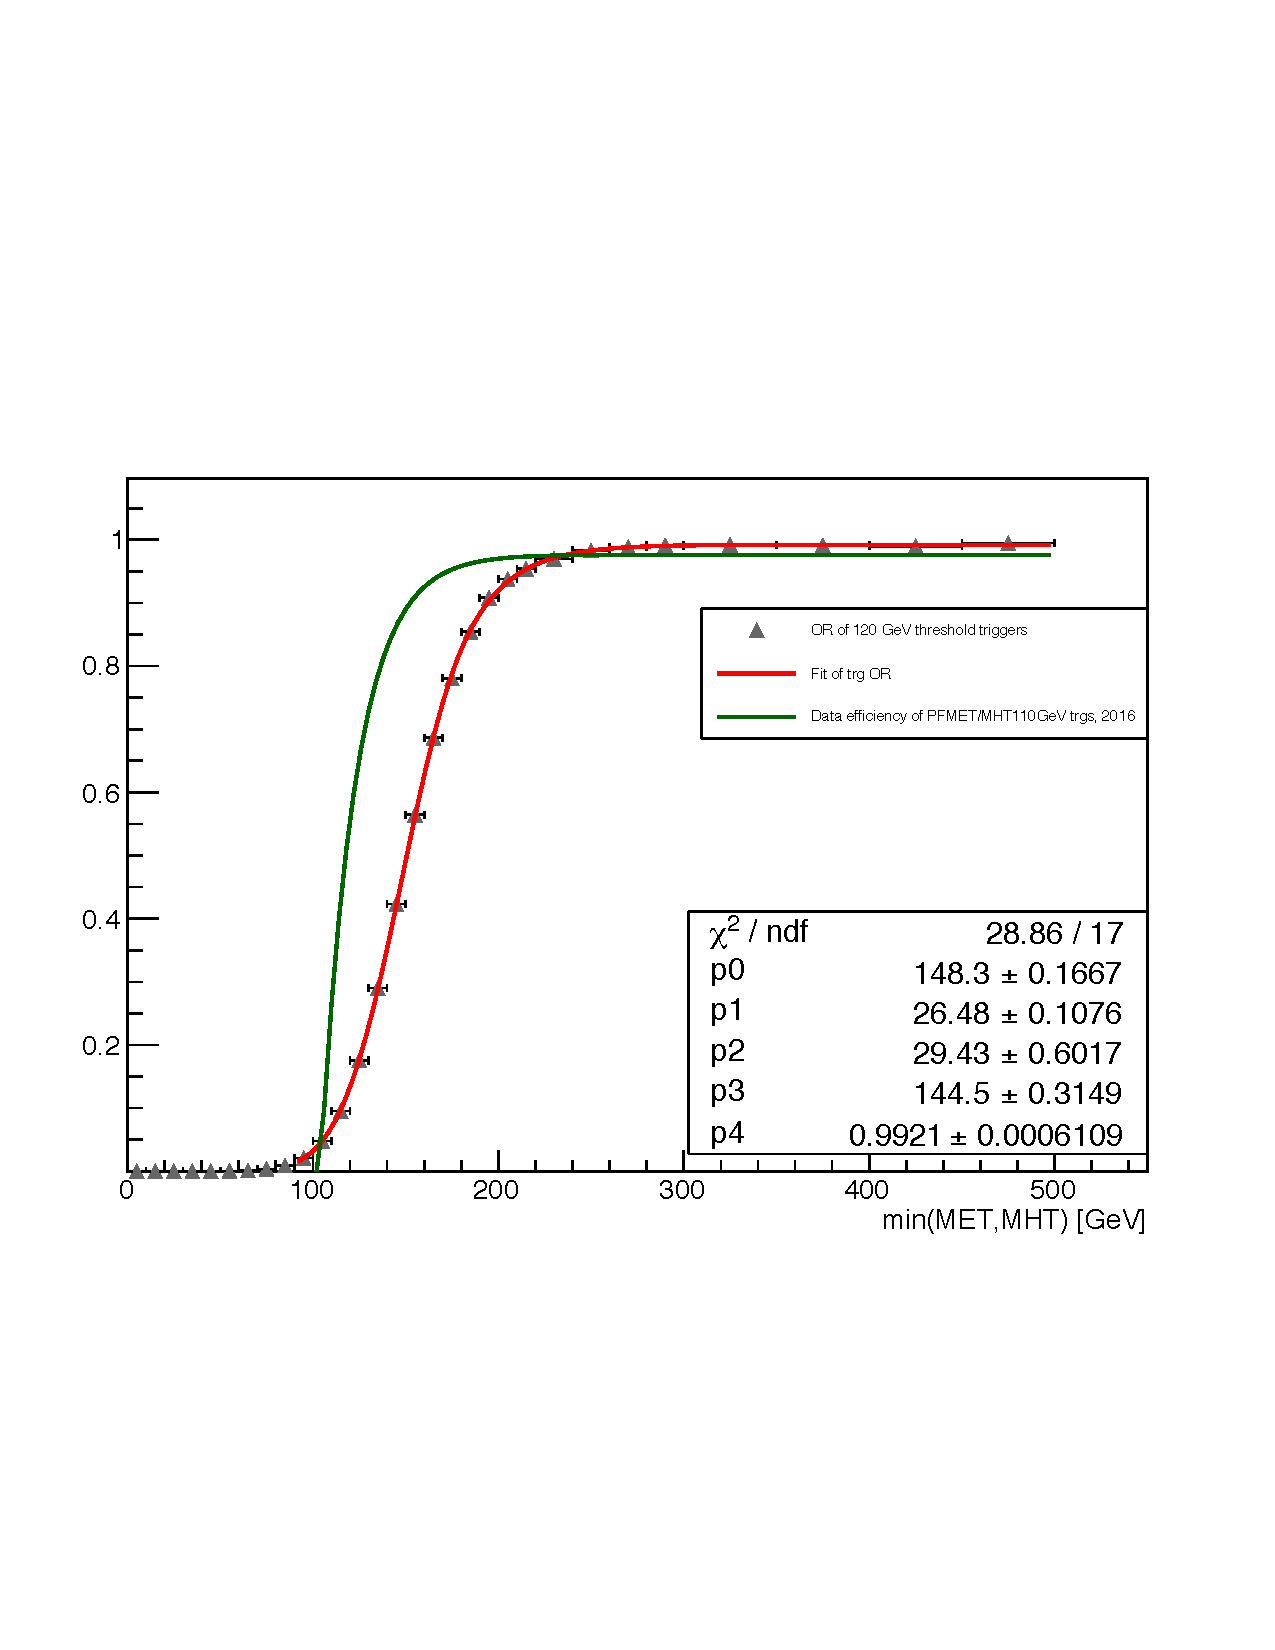
\includegraphics[width=3.75in]{images/2017METTriggersData}
    \caption[Trigger Efficiency for \ZnnHbb\ in 2017 Data]{The trigger efficiency for the \ZnnHbb\ channel as a function of the minimum of the offline MET and MHT measured using the full 2017 SingleElectron primary dataset. The green curve represents the efficiency in 2016 data of the logical \texttt{OR} of analogous triggers used by the 2016 analysis. The red curve represents the efficiency of the logical \texttt{OR} of the triggers used for the 2017 analysis.}
    \label{fig:triggersdata}
\end{figure}

The MET trigger efficiency can also be measured using MC samples to assess the trigger emulation performance. The trigger efficiency curve of the emulated MET triggers is obtained using the same procedure as for data and is shown in Figure \ref{fig:triggersmc}. An efficiency correction is obtained by taking the ratio of the fitted trigger efficiency curve for data to that of simulation and is shown in Figure \ref{fig:triggersunc}. The correction reaches up to 9\% in the ``turn-on'' region of the efficiency curve, but then remains close to unity upon reaching the plateau. The uncertainty of this efficiency correction were determined by the eigenvector decomposition of the covariance matrices of the fitted functions for data and simulation, and those which have non-negligible effects on the shape of the final discriminant or process normalizations are assessed as systematic uncertainties.

\begin{figure}[htbp]
  \centering
    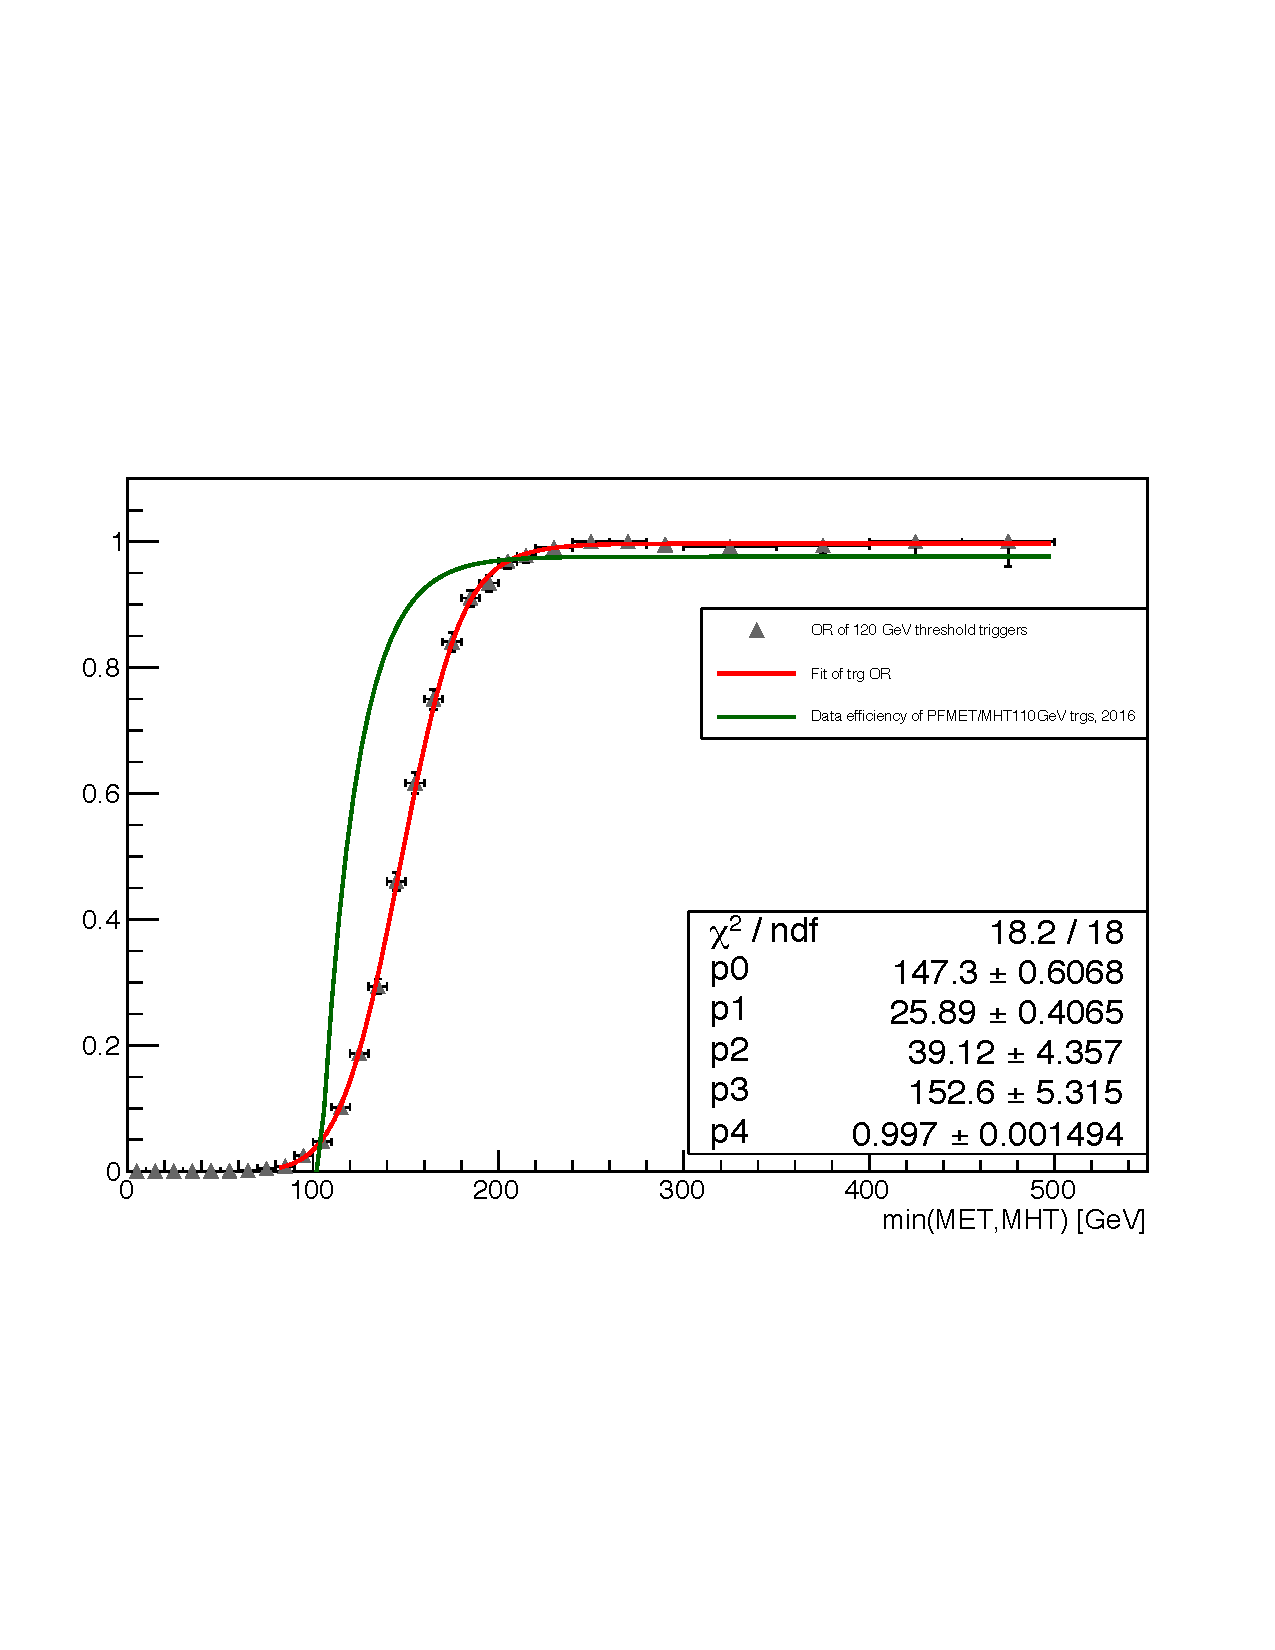
\includegraphics[width=3.75in]{images/2017METTriggersMC}
    \caption[Trigger Efficiency for \ZnnHbb\ in 2017 MC]{The emulated trigger efficiency for the \ZnnHbb\ channel as a function of the minimum of the offline MET and MHT measured using a $\bosW + 3\textrm{-jets}$ Monte-Carlo sample. The green curve represents the efficiency in 2016 data of the logical \texttt{OR} of analogous triggers used by the 2016 analysis. The red curve represents the efficiency of the emulated logical \texttt{OR} of the triggers used for the 2017 analysis.}
    \label{fig:triggersmc}
\end{figure}

\begin{figure}[htbp]
  \centering
  \mbox{
    \subfigure [] {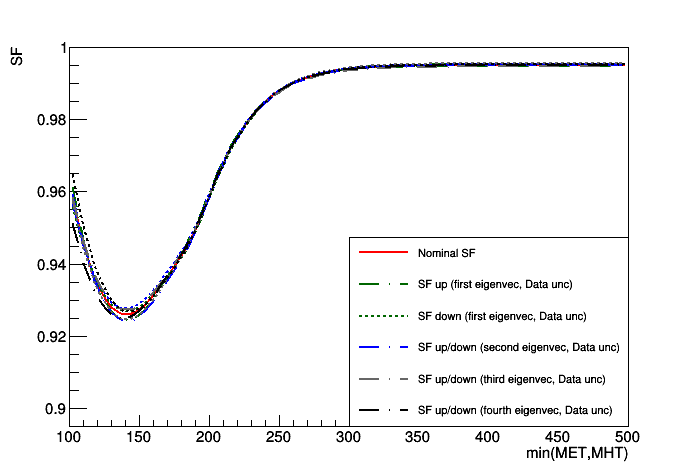
\includegraphics[scale=0.33]{images/metTrigger2017SF_dataunc}} \quad
    \subfigure [] {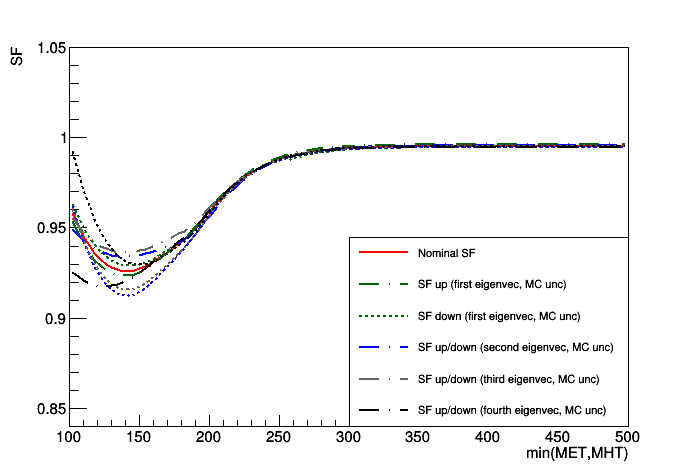
\includegraphics[scale=0.33]{images/metTrigger2017SF_mcunc}} \quad
  }
  \caption[2017 MET Trigger Efficiency Correction for \ZnnHbb]{The MET trigger efficiency correction for the \ZnnHbb\ channel as a function of the minimum of the offline MET and MHT. The red curve represents the nominal correction, while the dotted and dash-dotted curves represent the variations in the correction due to the four leading uncertainties in data (A) and Monte-Carlo (B).}
    \label{fig:triggersunc}
\end{figure}

The trigger efficiencies for the other decays channels are similarly handled. The triggers used by the \WlnH\ channel reach efficiencies of approximately 90\% for electrons and 95\% for muons. The triggers used by the \ZllH\ channel reach efficiencies of approximately 96\% for electrons and 91\% for muons.

\subsection{Residual Monte-Carlo Corrections}

Although the MC samples provide realistic simulations of physics processes, discrepancies between the shapes of kinematic distributions in data and MC remain a concern. The presence of such observed differences is not unexpected, given the fixed-order accuracy of and the assumptions made by the event generators. Residual corrections therefore need to be applied to the MC samples to improve the agreement between data and MC for key distributions.

The first such correction addresses the difference between the \pTV\ spectrum in data and the \bosV+jets MC samples. The \pTV\ distribution is harder for simulation than for data because the simulation does not include higher-order electroweak corrections.\cite{EWKCORR} The \bosV+jets samples are therefore reweighted as a function of the \pTV\ to apply the NLO electroweak correction shown in Figure \ref{fig:vjetsewkweight} which accounts for discrepancies of up to 10\% for \pTV\ near 400 \GeV.

\begin{figure}[htbp]
  \centering
    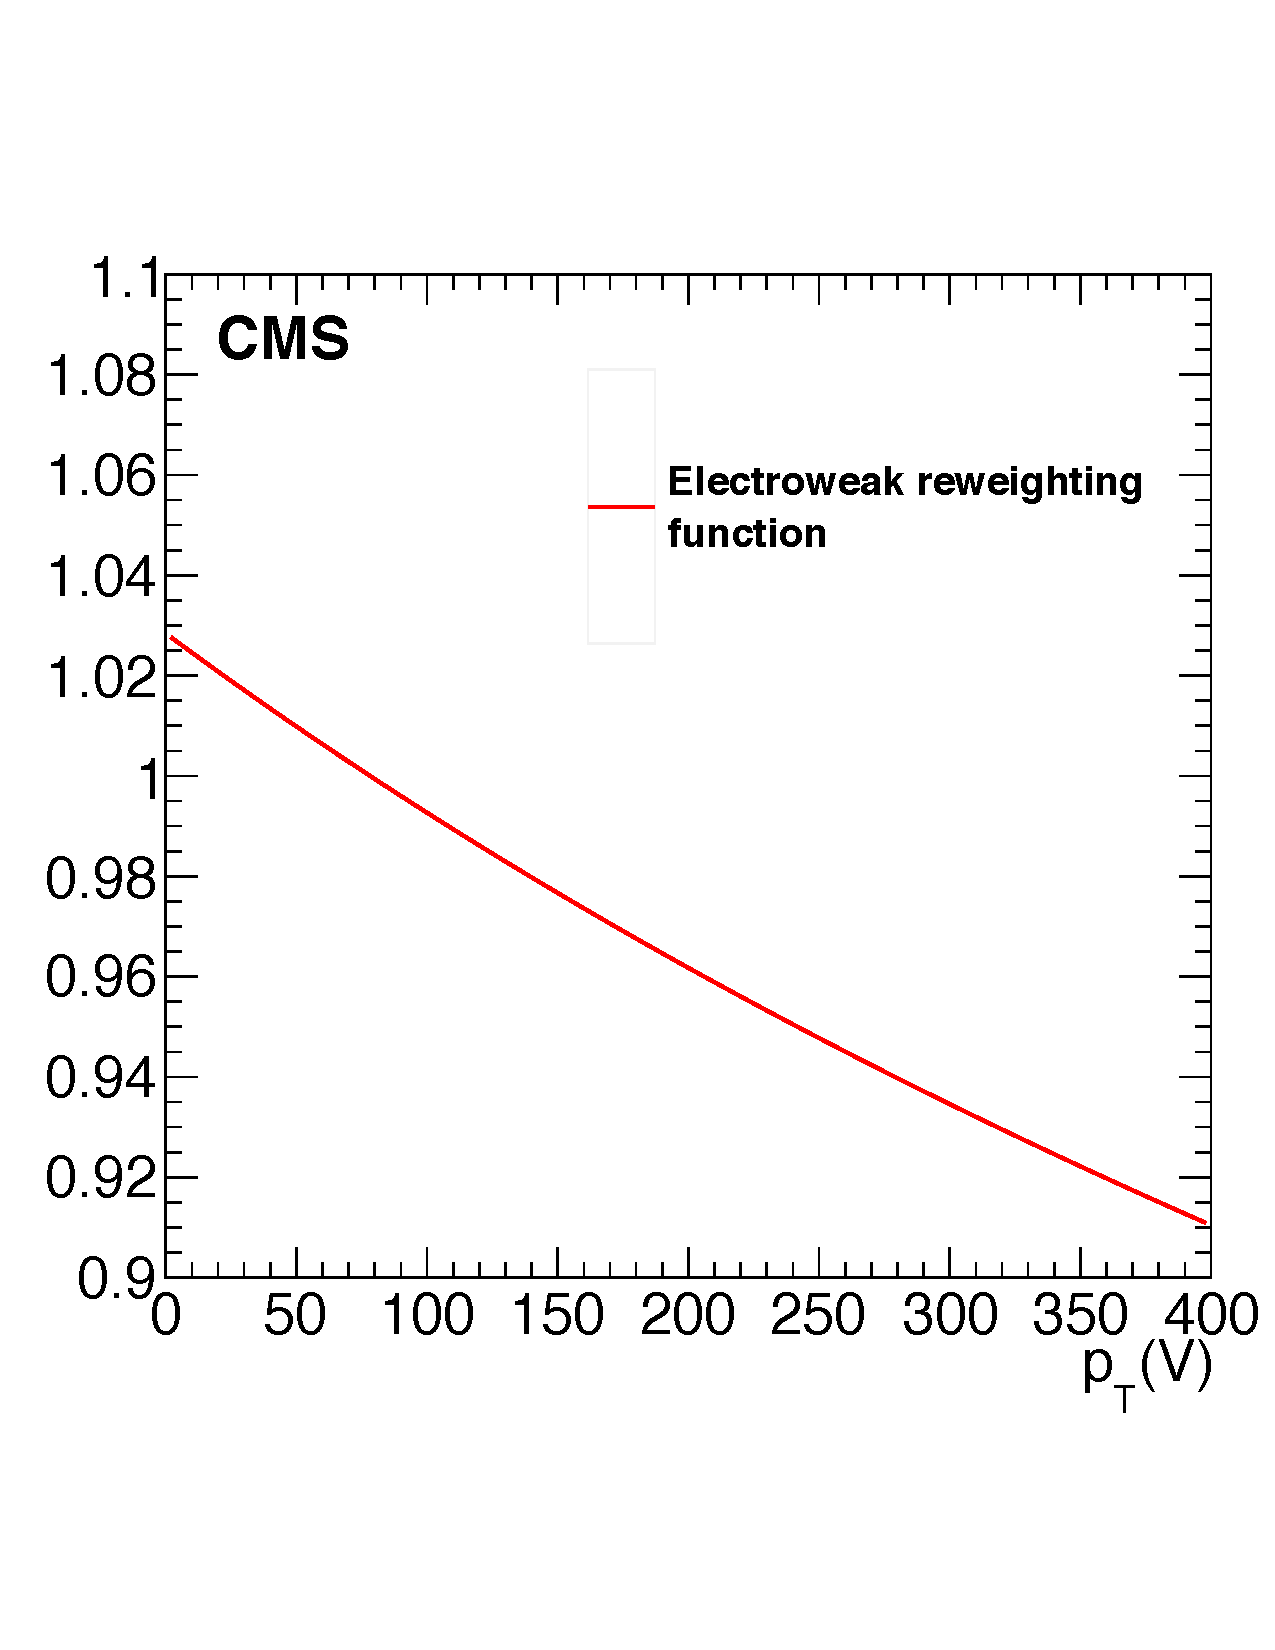
\includegraphics[width=3in]{images/ewk_vjets_correction}
    \caption[2017 \bosV+jets MC Electroweak Correction]{The NLO electroweak correction applied to the \bosV+jets Monte-Carlo samples.}
    \label{fig:vjetsewkweight}
\end{figure}

The second such correction addresses the difference between the \pT\ spectra of the top quarks in data and the $\qrkt\bar{\qrkt}$ MC samples. The \pT\ spectra of top quarks in data are observed to be softer than predicted by the event generators. The $\qrkt\bar{\qrkt}$ samples are therefore reweighted as a function of the top quark \pT\ according to the official recommendation by the CMS experiment.\cite{CMSTTCORR} This correction is only applicable for the \ZnnH\ and \ZllH\ channels, and is superceded by an equivalent reweighting specific to the \WlnH\ channel. 

A third correction addresses the discrepancy between the di-jet invariant mass \mjj\ distribution in data and the LO \bosV+jets MC samples. Although NLO \bosV+jets MC samples are readily available and show good agreement with data for the \mjj\ distribution, they are not used by the analysis because their limited statistical power results in an over 10\% decrease in expected sensitivity with respect to the LO \bosV+jets samples. A differential LO-to-NLO correction based on the separation in $\eta$ between the two \qrkb-quark jets from the Higgs boson decay $\Delta\eta(jj)$ is derived as a ratio of the NLO to LO \bosV+jets samples following the procedure outlined in Ref. \cite{CMSVHbbEvidence}. An example of this ratio is shown in Figure \ref{fig:NLOtoLOratio}. These reweighting functions improve the agreement between data and the LO \bosV+jets samples for the \mjj\ and \pTV\ distributions while demonstrating a negligible effect on the remaining distributions. The full reweighting is assessed as a systematic uncertainty.

\begin{figure}[htbp]
  \centering
    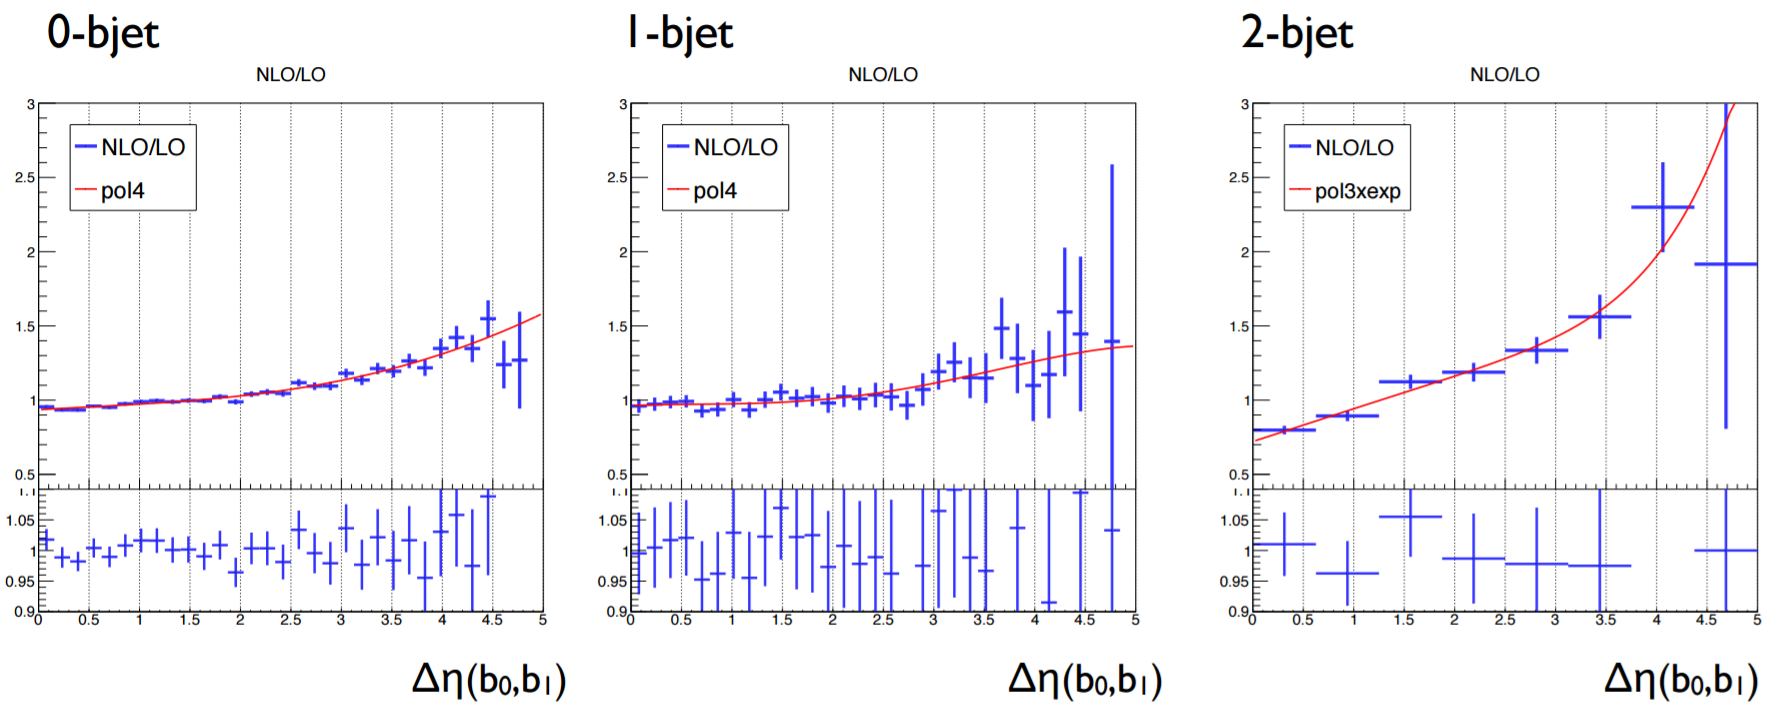
\includegraphics[width=6in]{images/NLOtoLO}
    \caption[NLO to LO Ratio of $\Delta\eta(jj)$ for \bosZ+jets $(\bosZ \rightarrow \ell\bar{\ell})$ Samples]{The ratio of $\Delta\eta(jj)$ between the NLO to LO \bosZ+jets $(\bosZ \rightarrow \ell\bar{\ell})$ Monte-Carlo samples divided into categories based on the number of true \qrkb-jets present.}
    \label{fig:NLOtoLOratio}
\end{figure}

A final correction addresses the downward trend in the data to MC ratio for the \pTV\ distribution that is observed in the control regions of the \WlnH\ channel. A simultaneous fit of the \pTV\ distribution to data in the control regions of the \WlnH\ channel are used to derive independent linear reweighting functions for the $\qrkt\bar{\qrkt}$, \bosW with light-flavored jets (\Wlight), and combination of \bosW with \qrkb-jets (\Wbb) and single top processes. The relative compositions of the background processes were fixed during the fit and the reweighting preserves the overall normalization. The uncertainties on the fitted slopes of the linear reweighting functions are taken to be the systematic uncertainties of this \pTV\ correction. An uncertainty of 13\% is assessed for the $\qrkt\bar{\qrkt}$ reweighting, while a 6\% uncertainty is asseseed for both the \Wlight and \Wbb + single top reweightings. These uncertainties sufficiently cover any perceived discrepancies after all corrections have been applied.

\section{Physics Objects}

\subsection{Vector Boson Candidate}

\subsection{Higgs Boson Candidate}

\section{Event Selection}

\subsection{Signal Regions}

\subsection{Background Control Regions}

\section{Binned Multivariate Shape Analysis}

\subsection{Input Features}

\subsection{Model Training}

\subsection{Model Selection}

\subsection{Binned Shape Analysis}

\section{Systematic Uncertainties}

%\section{Non Porttitor Tellus}
%
%Aliquam molestie sed urna quis convallis. Aenean nibh eros, aliquam non eros in, tempus lacinia justo. In magna sapien, blandit a faucibus ac, scelerisque nec purus. Praesent fermentum felis nec massa interdum, vel dapibus mi luctus. Cras id fringilla mauris. Ut molestie eros mi, ut hendrerit nulla tempor et. Pellentesque tortor quam, mattis a scelerisque nec, euismod et odio. Mauris rhoncus metus sit amet risus mattis, eu mattis sem interdum.
%
%\subsection{Nam Arcu Magna}
%Semper vel lorem eu, venenatis ultrices est. Nam aliquet ut erat ac scelerisque. Maecenas ut molestie mi. Phasellus ipsum magna, sollicitudin eu ipsum quis, imperdiet cursus turpis. Etiam pretium enim a fermentum accumsan. Morbi vel vehicula enim.
%
%\subsubsection{Ut pellentesque velit sede}
% Placerat cursus. Integer congue urna non massa dictum, a pellentesque arcu accumsan. Nulla posuere, elit accumsan eleifend elementum, ipsum massa tristique metus, in ornare neque nisl sed odio. Nullam eget elementum nisi. Duis a consectetur erat, sit amet malesuada sapien. Aliquam nec sapien et leo sagittis porttitor at ut lacus. Vivamus vulputate elit vitae libero condimentum dictum. Nulla facilisi. Quisque non nibh et massa ullamcorper iaculis.
%

%\chapter{RESULTS} \label{results}

The principle results reported by this analysis are the discovery significance and an estimate of the signal strength $\mu$ of the \VHbb\ decay. The discovery significance is the statistical significance of any observed excess of events in data over the expected SM background. The signal strength is defined as the measured production cross section times the \Htobb\ branching fraction divided by the expected SM value or $\sigma / \sigma_{\textrm{SM}}$. The statistical analysis was performed using the \textsc{combine}\cite{HIGGSCOMBINE} software package developed by the CMS collaboration which provides a command line interface for the statistical tools implemented in \textsc{RooFit}\cite{ROOFIT} and \textsc{RooStats}\cite{ROOSTATS}.

\section{Statistical Treatment}

The discovery significance is computed using the profile likelihood asymptotic approximation.\cite{STATS1,FITRES2,FITRES3,FITRES4} In this approach, the significance is calculated from a profile likelihood ratio where the signal strength is set to zero in the numerator and is allowed to float freely in the denominator. The test statistic defined by the profile likelihood ratio is thus
\begin{equation}
  q_{0} = -2 \ln \frac{\mathcal{L}\left( \textrm{data} | b, \hat{\theta}_{0} \right)}{\mathcal{L}\left( \textrm{data} | \hat{\mu} \times s + b, \hat{\theta} \right)}\ \mathrm{for}\ \hat{\mu} > 0,
  \label{eq:proflikeapprox}
\end{equation}
where $\textrm{data}$ comes from either the observed dataset when calculating the observed significance or a generated toy dataset when calculating the expected significance, $s$ and $b$ are respectively the expected number and distribution of signal and background events, $\hat{\theta}_{0}$ is the estimated value of the nuisance parameter that maximizes the likelihood of the numerator, and $\hat{\mu}$ and $\hat{\theta}$ are the estimated values of the signal strength and nuisance parameter that maximizes the likelihood of the denominator. The value of $\hat{\mu}$ is restricted to be positive to remain physically meaningful. Assuming that the number of events is large, the distribution of this test statistic may be determined asymptotically using Wilke's theorem.

The local $p$-value is defined as the probability of obtaining a value of $q_{0}$ greater than or equal to the value of $q_{0}$ observed in data under the background-only hypothesis such that
\begin{equation}
  p_{0} = P\left( q_{0} \geq q_{0}^{\textrm{data}} | b \right).
  \label{eq:localpvalue}
\end{equation}
The value of $p_{0}$ is therefore a measure of the probability that an upward fluctuation of the background is responsible for an observed excess of events in the absence of signal. Each value of $p_{0}$ corresponds to a unique level of significance $z$ that is computed from the right-sided tail of a standard normal distribution
\begin{equation}
  p_{0} = \frac{1}{\sqrt{2\pi}} \int_{z}^{+\infty} e^{-\frac{1}{2} x^{2}} dx.
  \label{eq:zscore}
\end{equation}
This discovery significance is typically quoted in terms of the number of standard deviations $\sigma$, with a threshold of $3\sigma$ ($z = 3$) required to establish evidence for a decay and a threshold of $5\sigma$ ($z = 5$) required to establish an observation of a decay.

In the presence of an excess of events, the best fit value of the estimated signal strength $\hat{\mu}$ is determined by a simultaneous binned maximum likelihood fit over the signal and control regions of all decay channels during which the signal strength $\hat{\mu}$ is allowed to vary freely and the nuisance parameters $\hat{\theta}$ vary within their uncertainties. For the \VHbb\ analysis, the signal extraction fit is performed using the DNN-based multivariate discriminants in the signal regions and the distributions of the subleading DeepCSV score of the two \qrkb-jets \btagmin\ in the control regions. The signal extraction fit for the \VZbb\ cross-check analysis proceeds in the same manner, with the only differences being a wider dijet invariant mass window in the signal region and a DNN classifier trained to identify diboson events as signal. For the dijet invariant mass cross-check analysis, the fit is performed using the dijet invariant mass distributions of the four distinct categories in the signal region of each decay channel while the control regions and their distributions remain the same as in the \VHbb\ analysis.

\section{\VZbb\ Analysis}

The data to MC scale factors obtained by the maximum likelihood fit are shown in Table \ref{tbl:SFVZbb}. The post-fit multivariate discriminant distributions of each channel are shown individually in Figure \ref{fig:SRVZbb} and combined in Figure \ref{fig:SBVZbb}. The expected post-fit significance of the excess over the background prediction is $5.0\sigma$, while the observed significance is $5.2\sigma$. The best fit signal strength is $\mu = 1.05_{-0.21}^{+0.22}$ for all channels combined and the signal strengths of the individual channels, shown in Figure \ref{fig:MuVZbb}, are compatible with a $p$-value of 64\%. These results are in good agreement with past measurements of the \VZbb\ process and the observation of this known Standard Model process serves as an important validation of the analysis strategy.

\begin{table}[htbp]
  \caption[\VZbb\ Analysis Scale Factors]{The data to Monte-Carlo scale factors obtained by the simultaneous maximum likelihood fit over all \VZbb\ channels. The errors include both statistical and systematic uncertainties.}
  \label{tbl:SFVZbb}
  \begin{tabularx}{6.5in}{lXXll}
    \hline
    Process       & \ZnnH           & \WlnH           & \ZllH, Low \pT(\bosV) & \ZllH, High \pT(\bosV) \\
    \hline
    \Wlight       & $1.04 \pm 0.01$ & $1.04 \pm 0.01$ & -                     & -                      \\
    \Wb           & $2.02 \pm 0.09$ & $2.02 \pm 0.09$ & -                     & -                      \\
    \Wbb          & $2.02 \pm 0.13$ & $2.02 \pm 0.13$ & -                     & -                      \\
    \Zlight       & $0.86 \pm 0.05$ & -               & $0.88 \pm 0.01$       & $0.80 \pm 0.01$        \\
    \Zb           & $1.07 \pm 0.14$ & -               & $0.89 \pm 0.05$       & $1.13 \pm 0.08$        \\
    \Zbb          & $1.20 \pm 0.07$ & -               & $0.84 \pm 0.03$       & $0.95 \pm 0.05$        \\
    \qrkt\qrktbar & $0.97 \pm 0.02$ & $0.93 \pm 0.01$ & $0.88 \pm 0.01$       & $0.90 \pm 0.02$        \\
    \hline
  \end{tabularx}
\end{table}

\begin{figure}[htbp]
  \centering
  \mbox{
    \subfigure [] {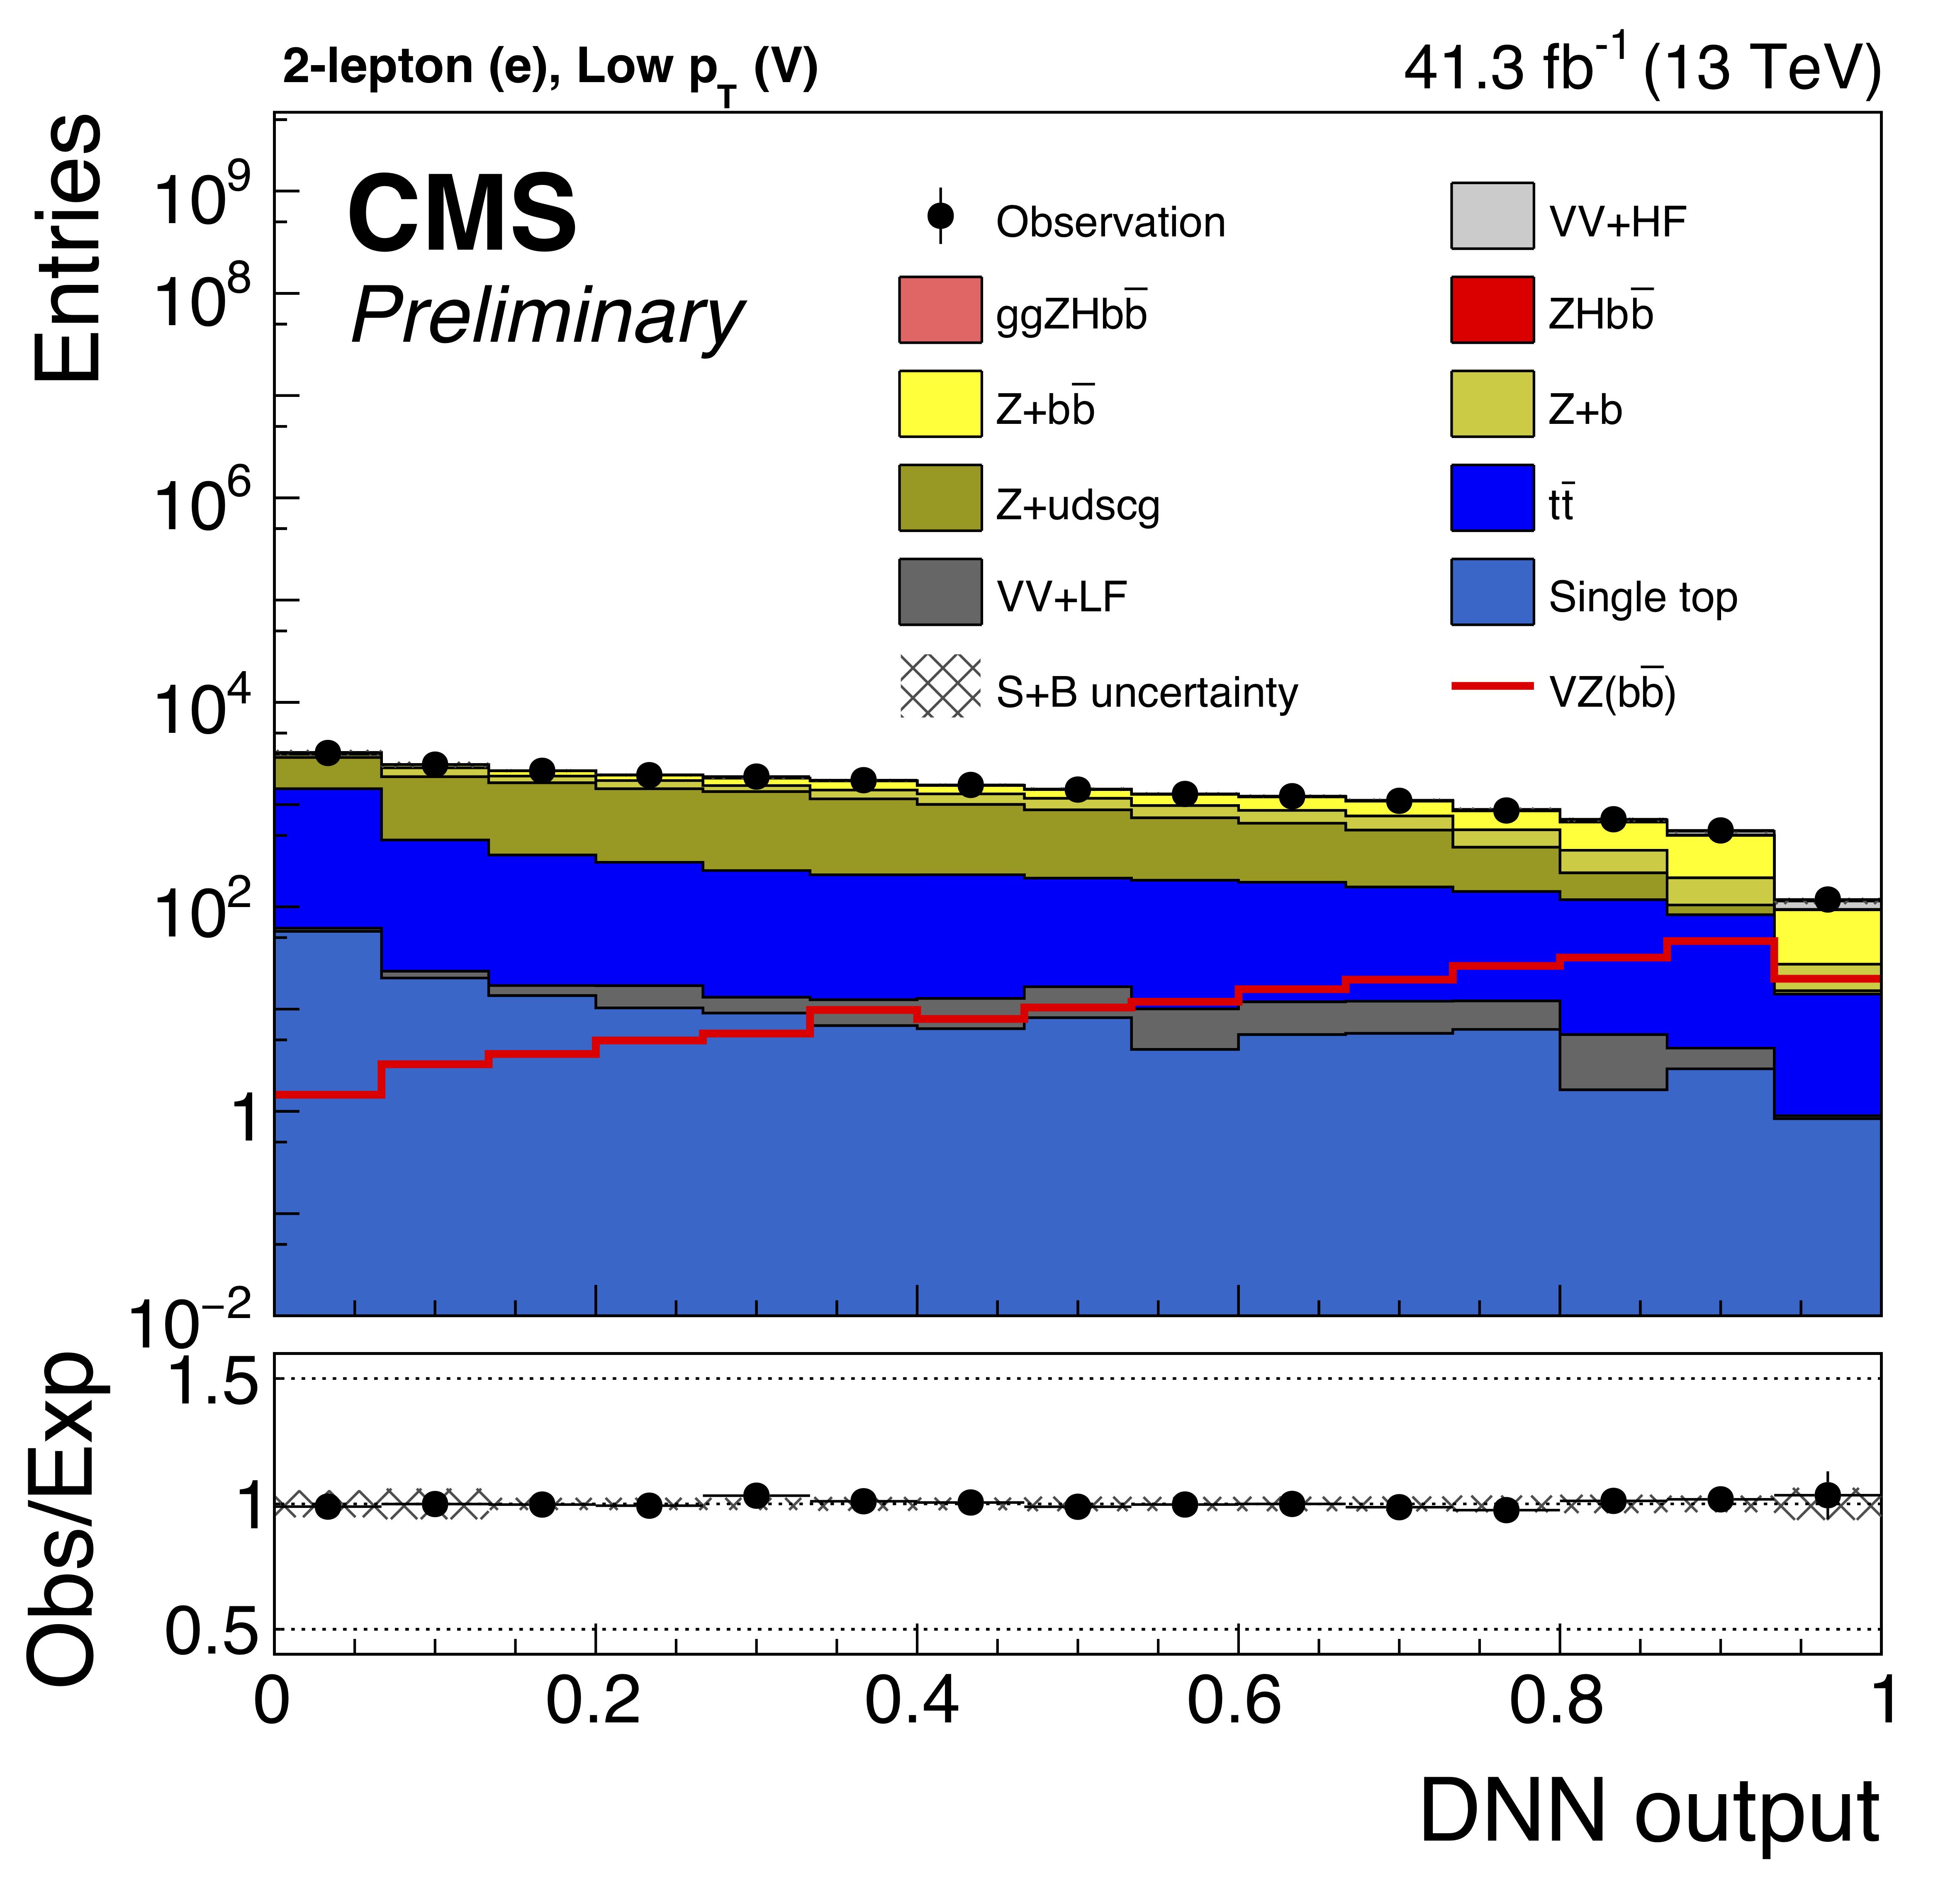
\includegraphics[width=0.285\linewidth]{images/SR_VZbb/vhbb_Zee_2_13TeV2017_shapes_postfit_logy}} \qquad
    \subfigure [] {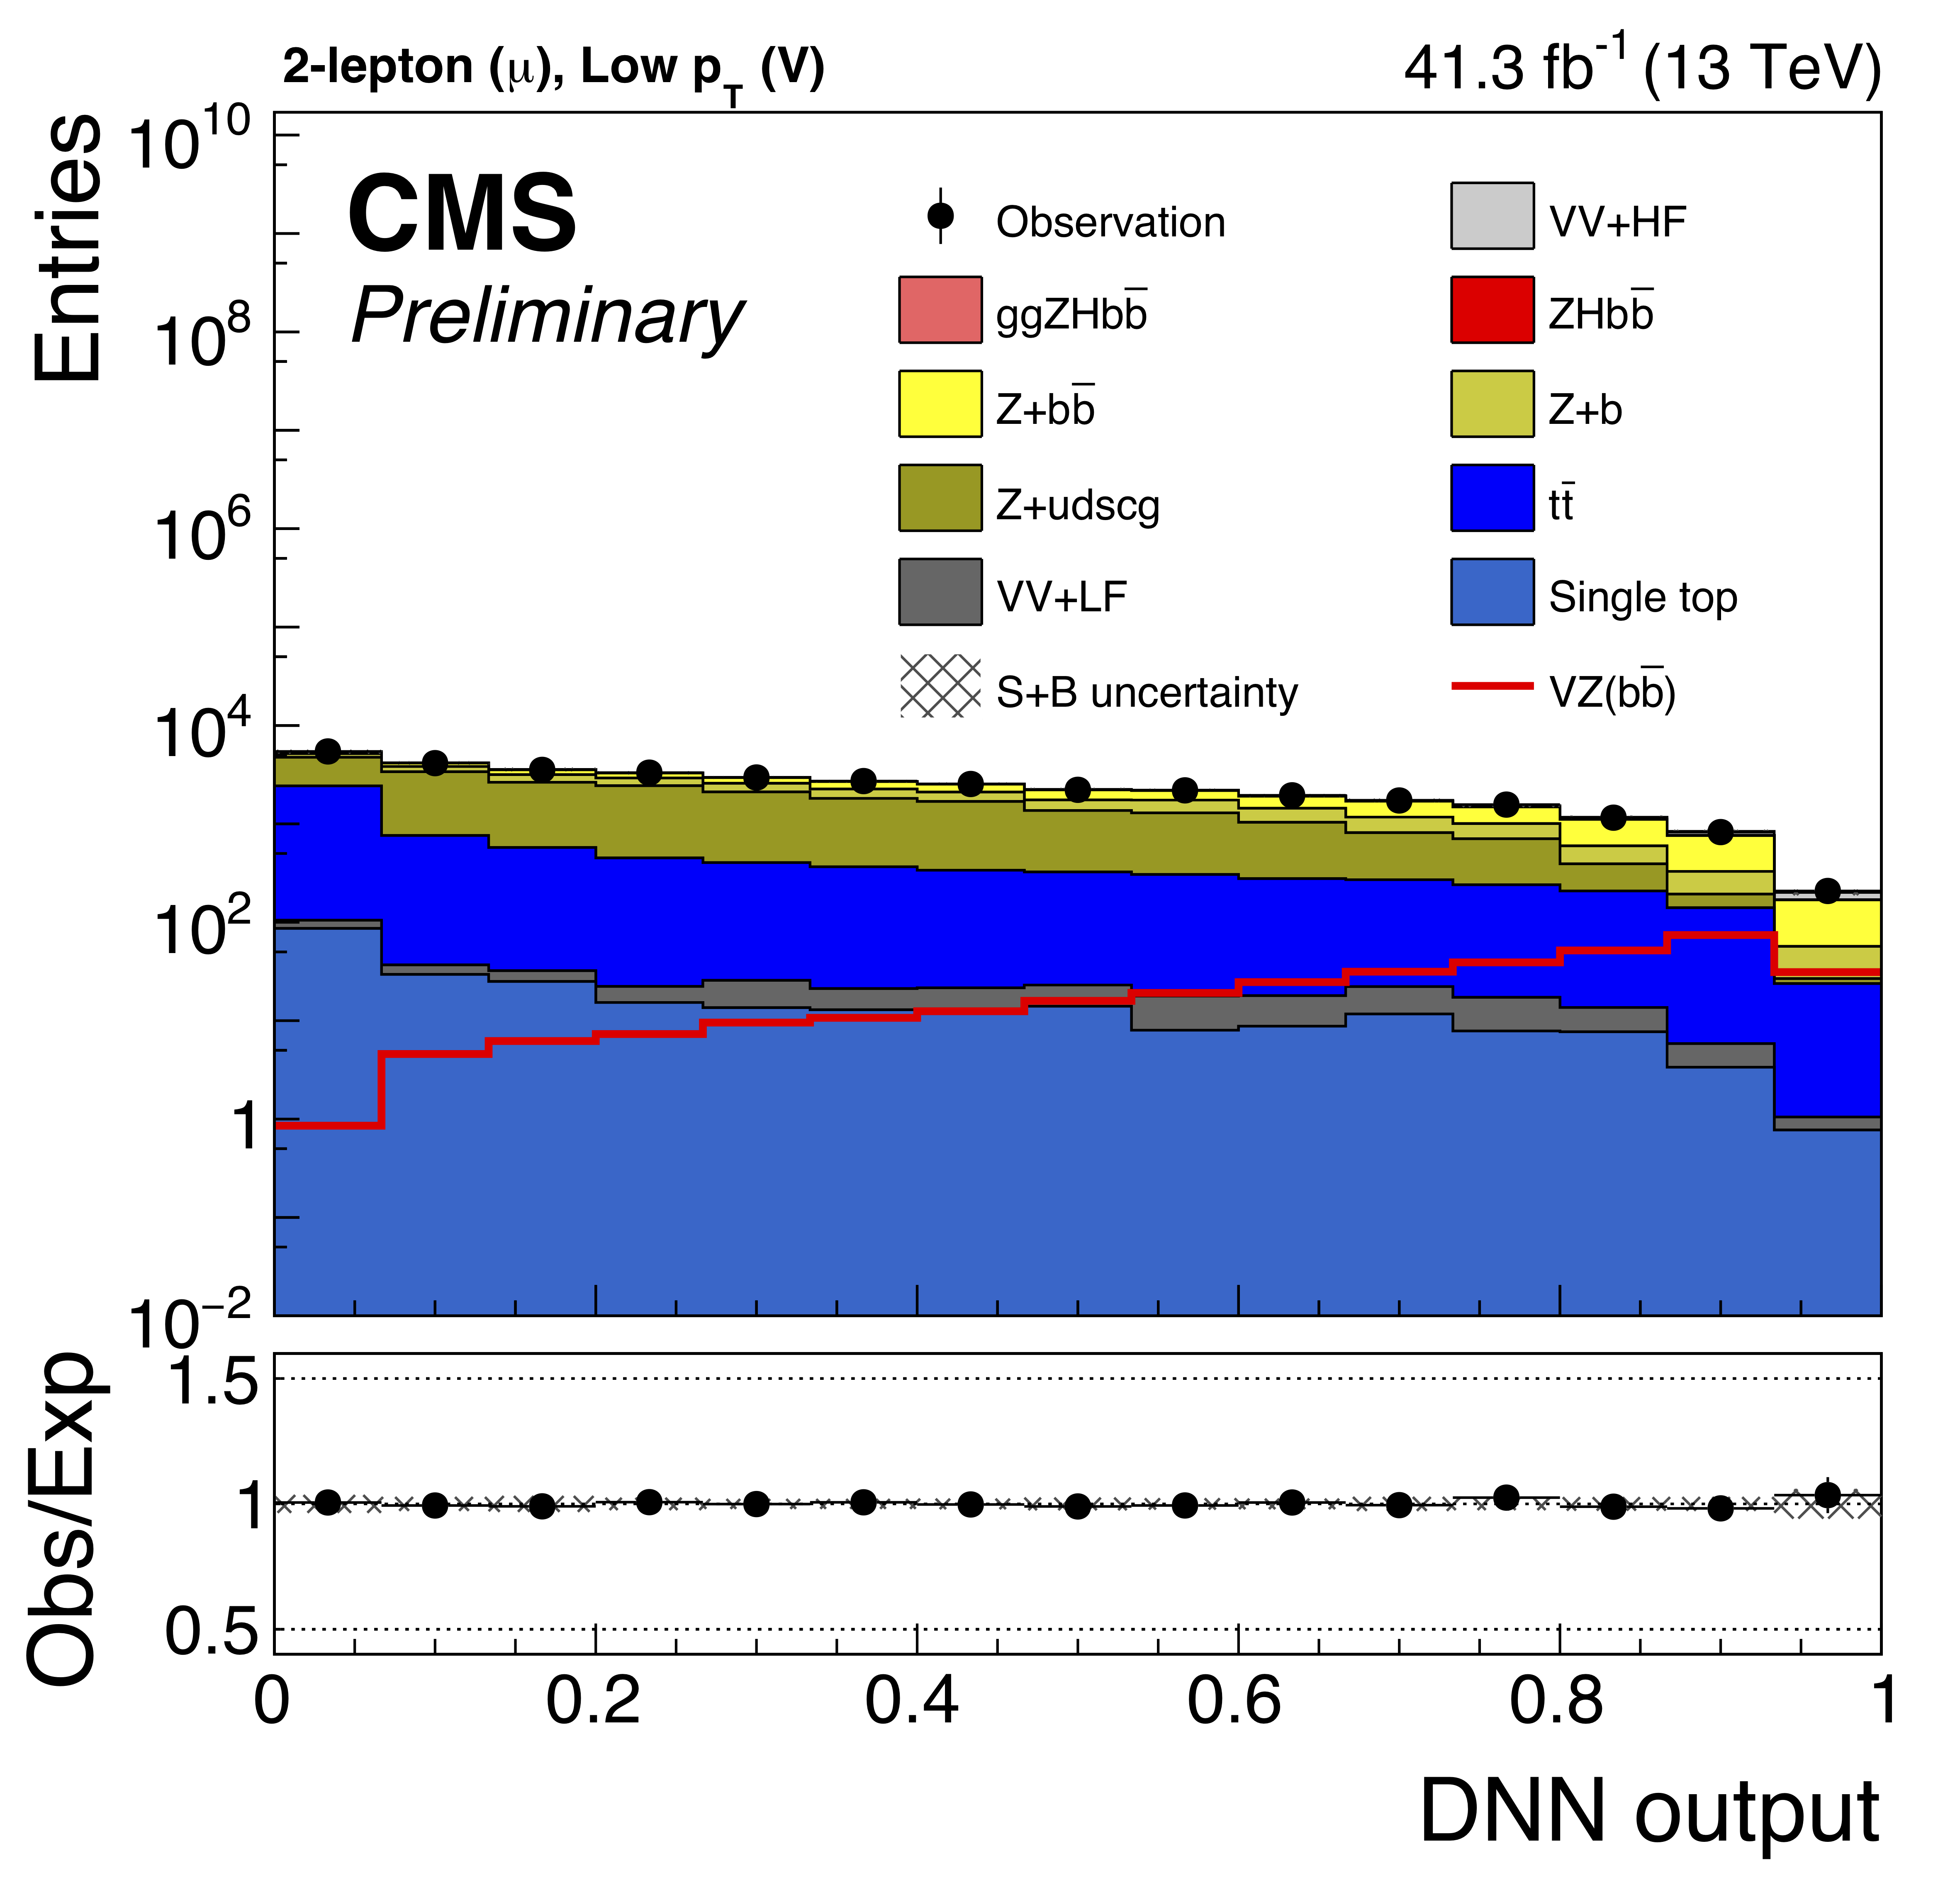
\includegraphics[width=0.285\linewidth]{images/SR_VZbb/vhbb_Zmm_2_13TeV2017_shapes_postfit_logy}} \qquad
  }
  \mbox{
    \subfigure [] {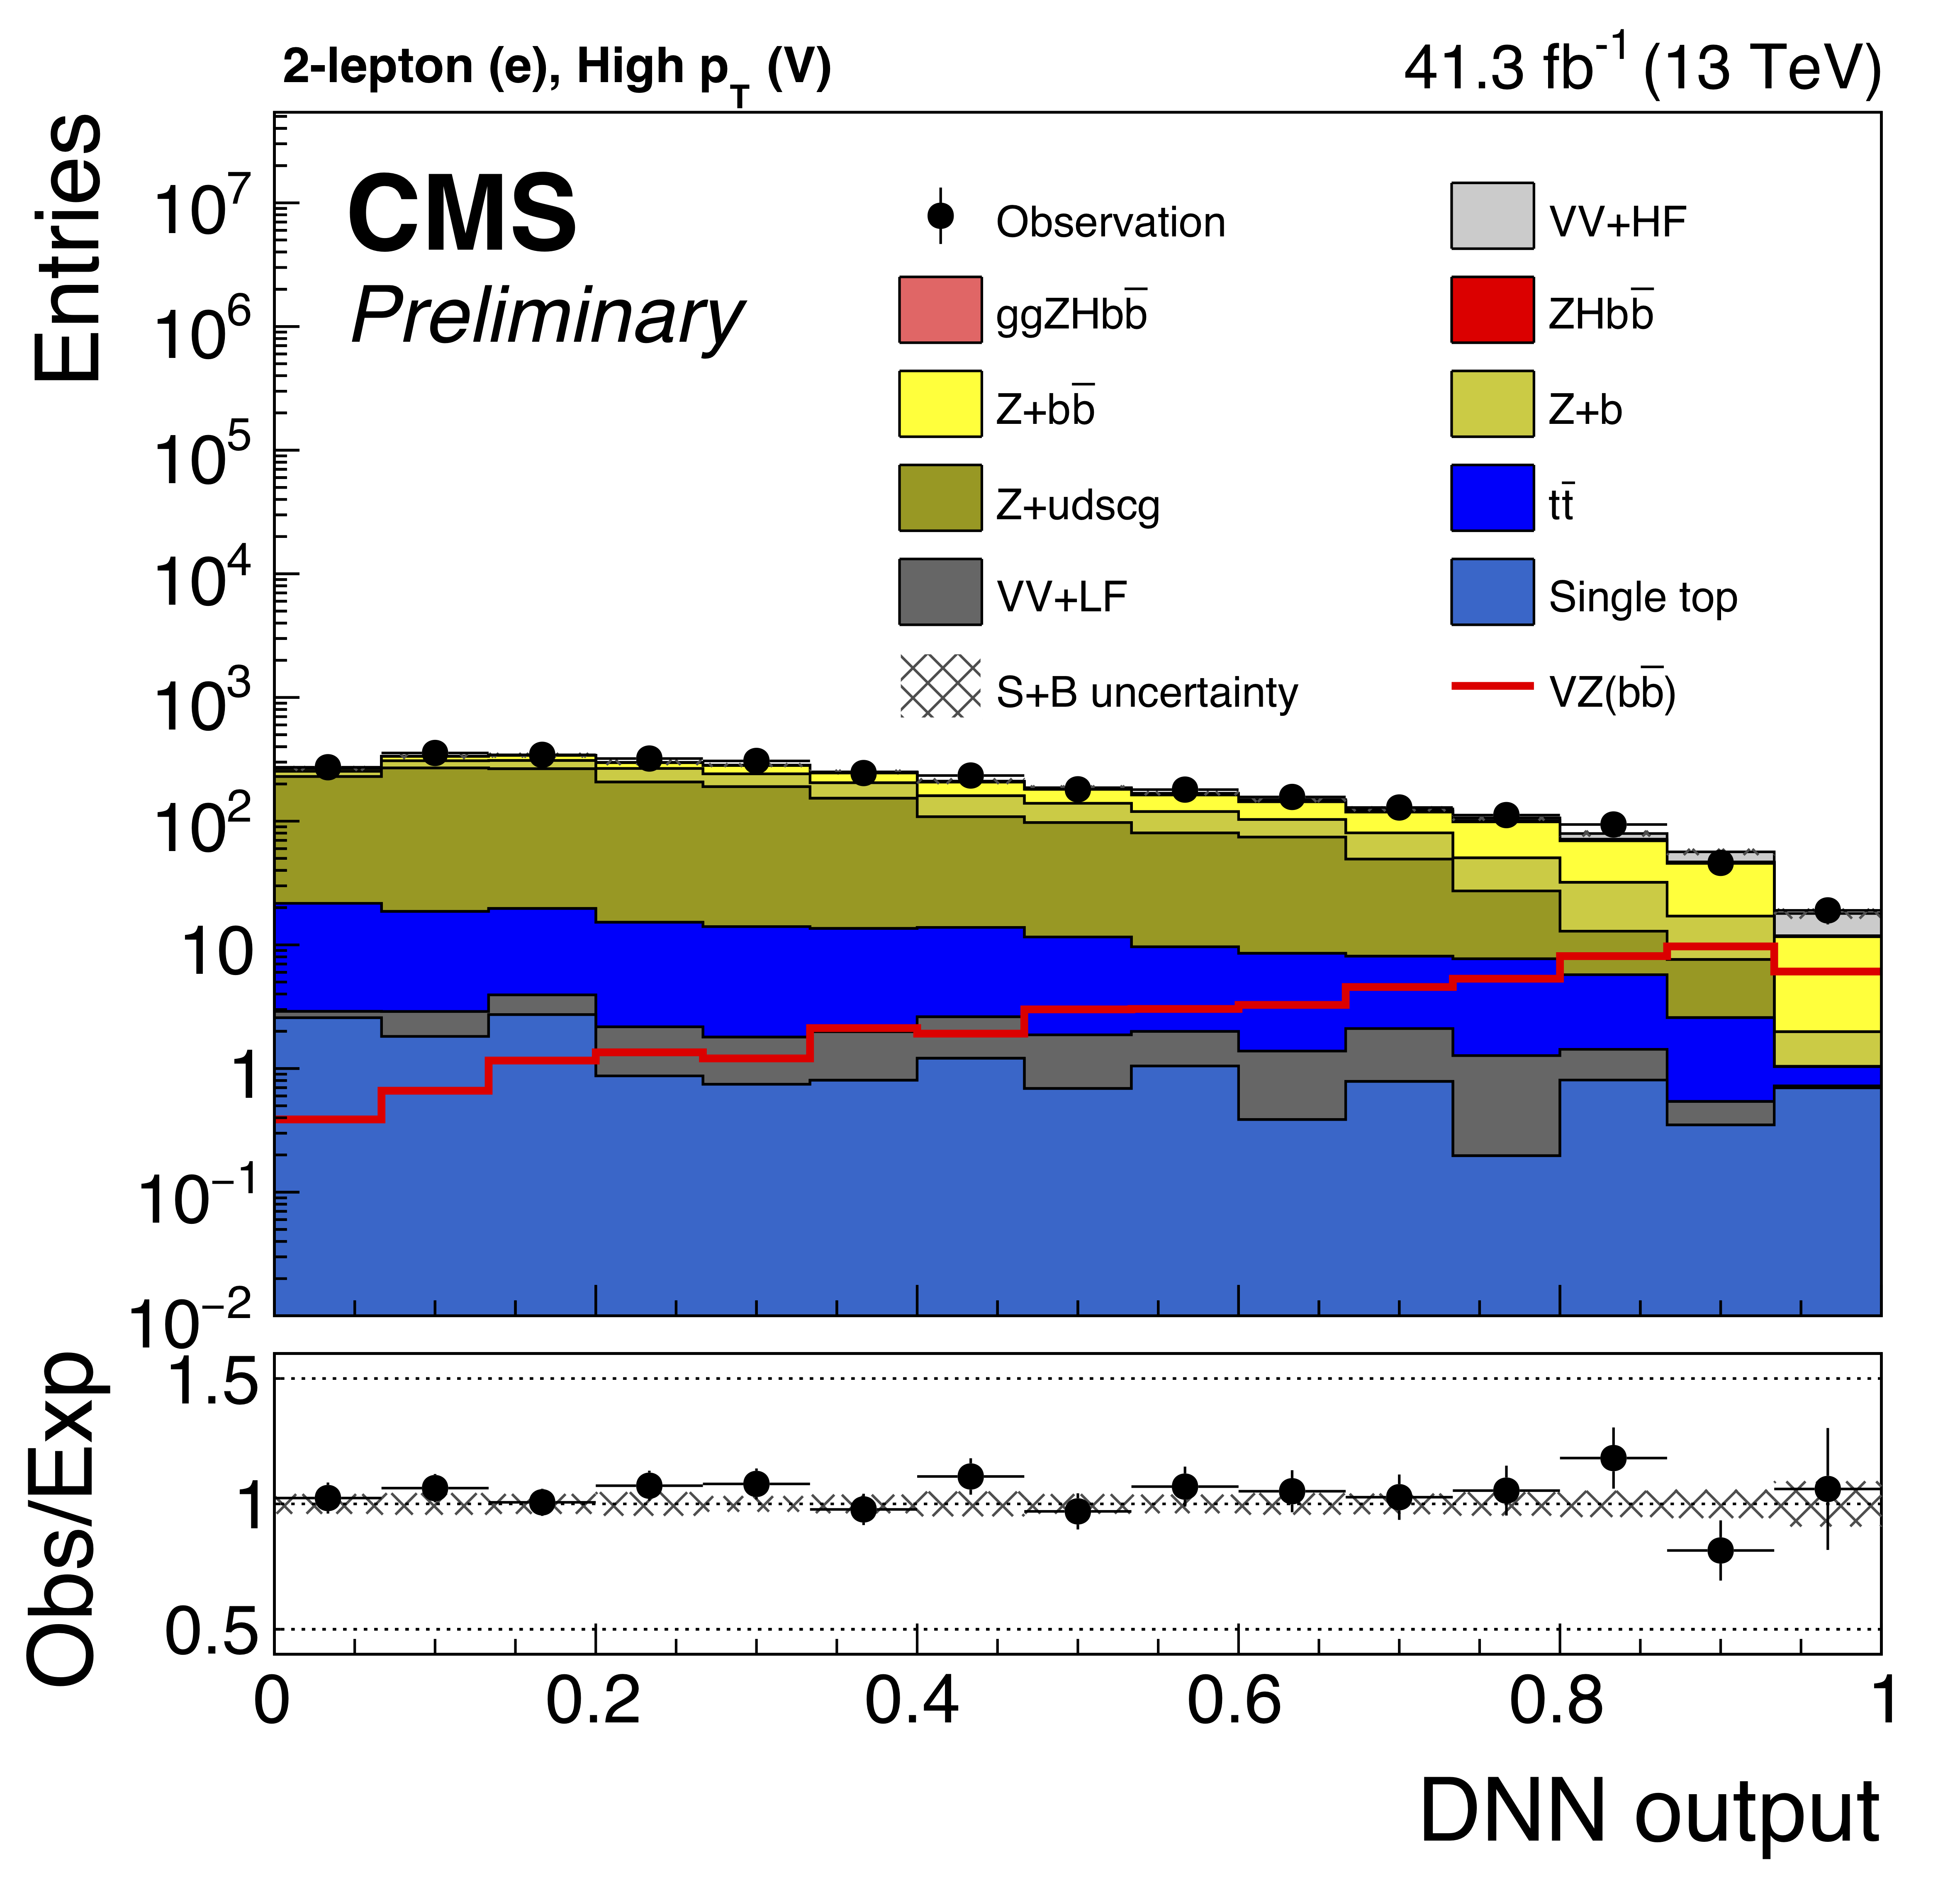
\includegraphics[width=0.285\linewidth]{images/SR_VZbb/vhbb_Zee_1_13TeV2017_shapes_postfit_logy}} \qquad
    \subfigure [] {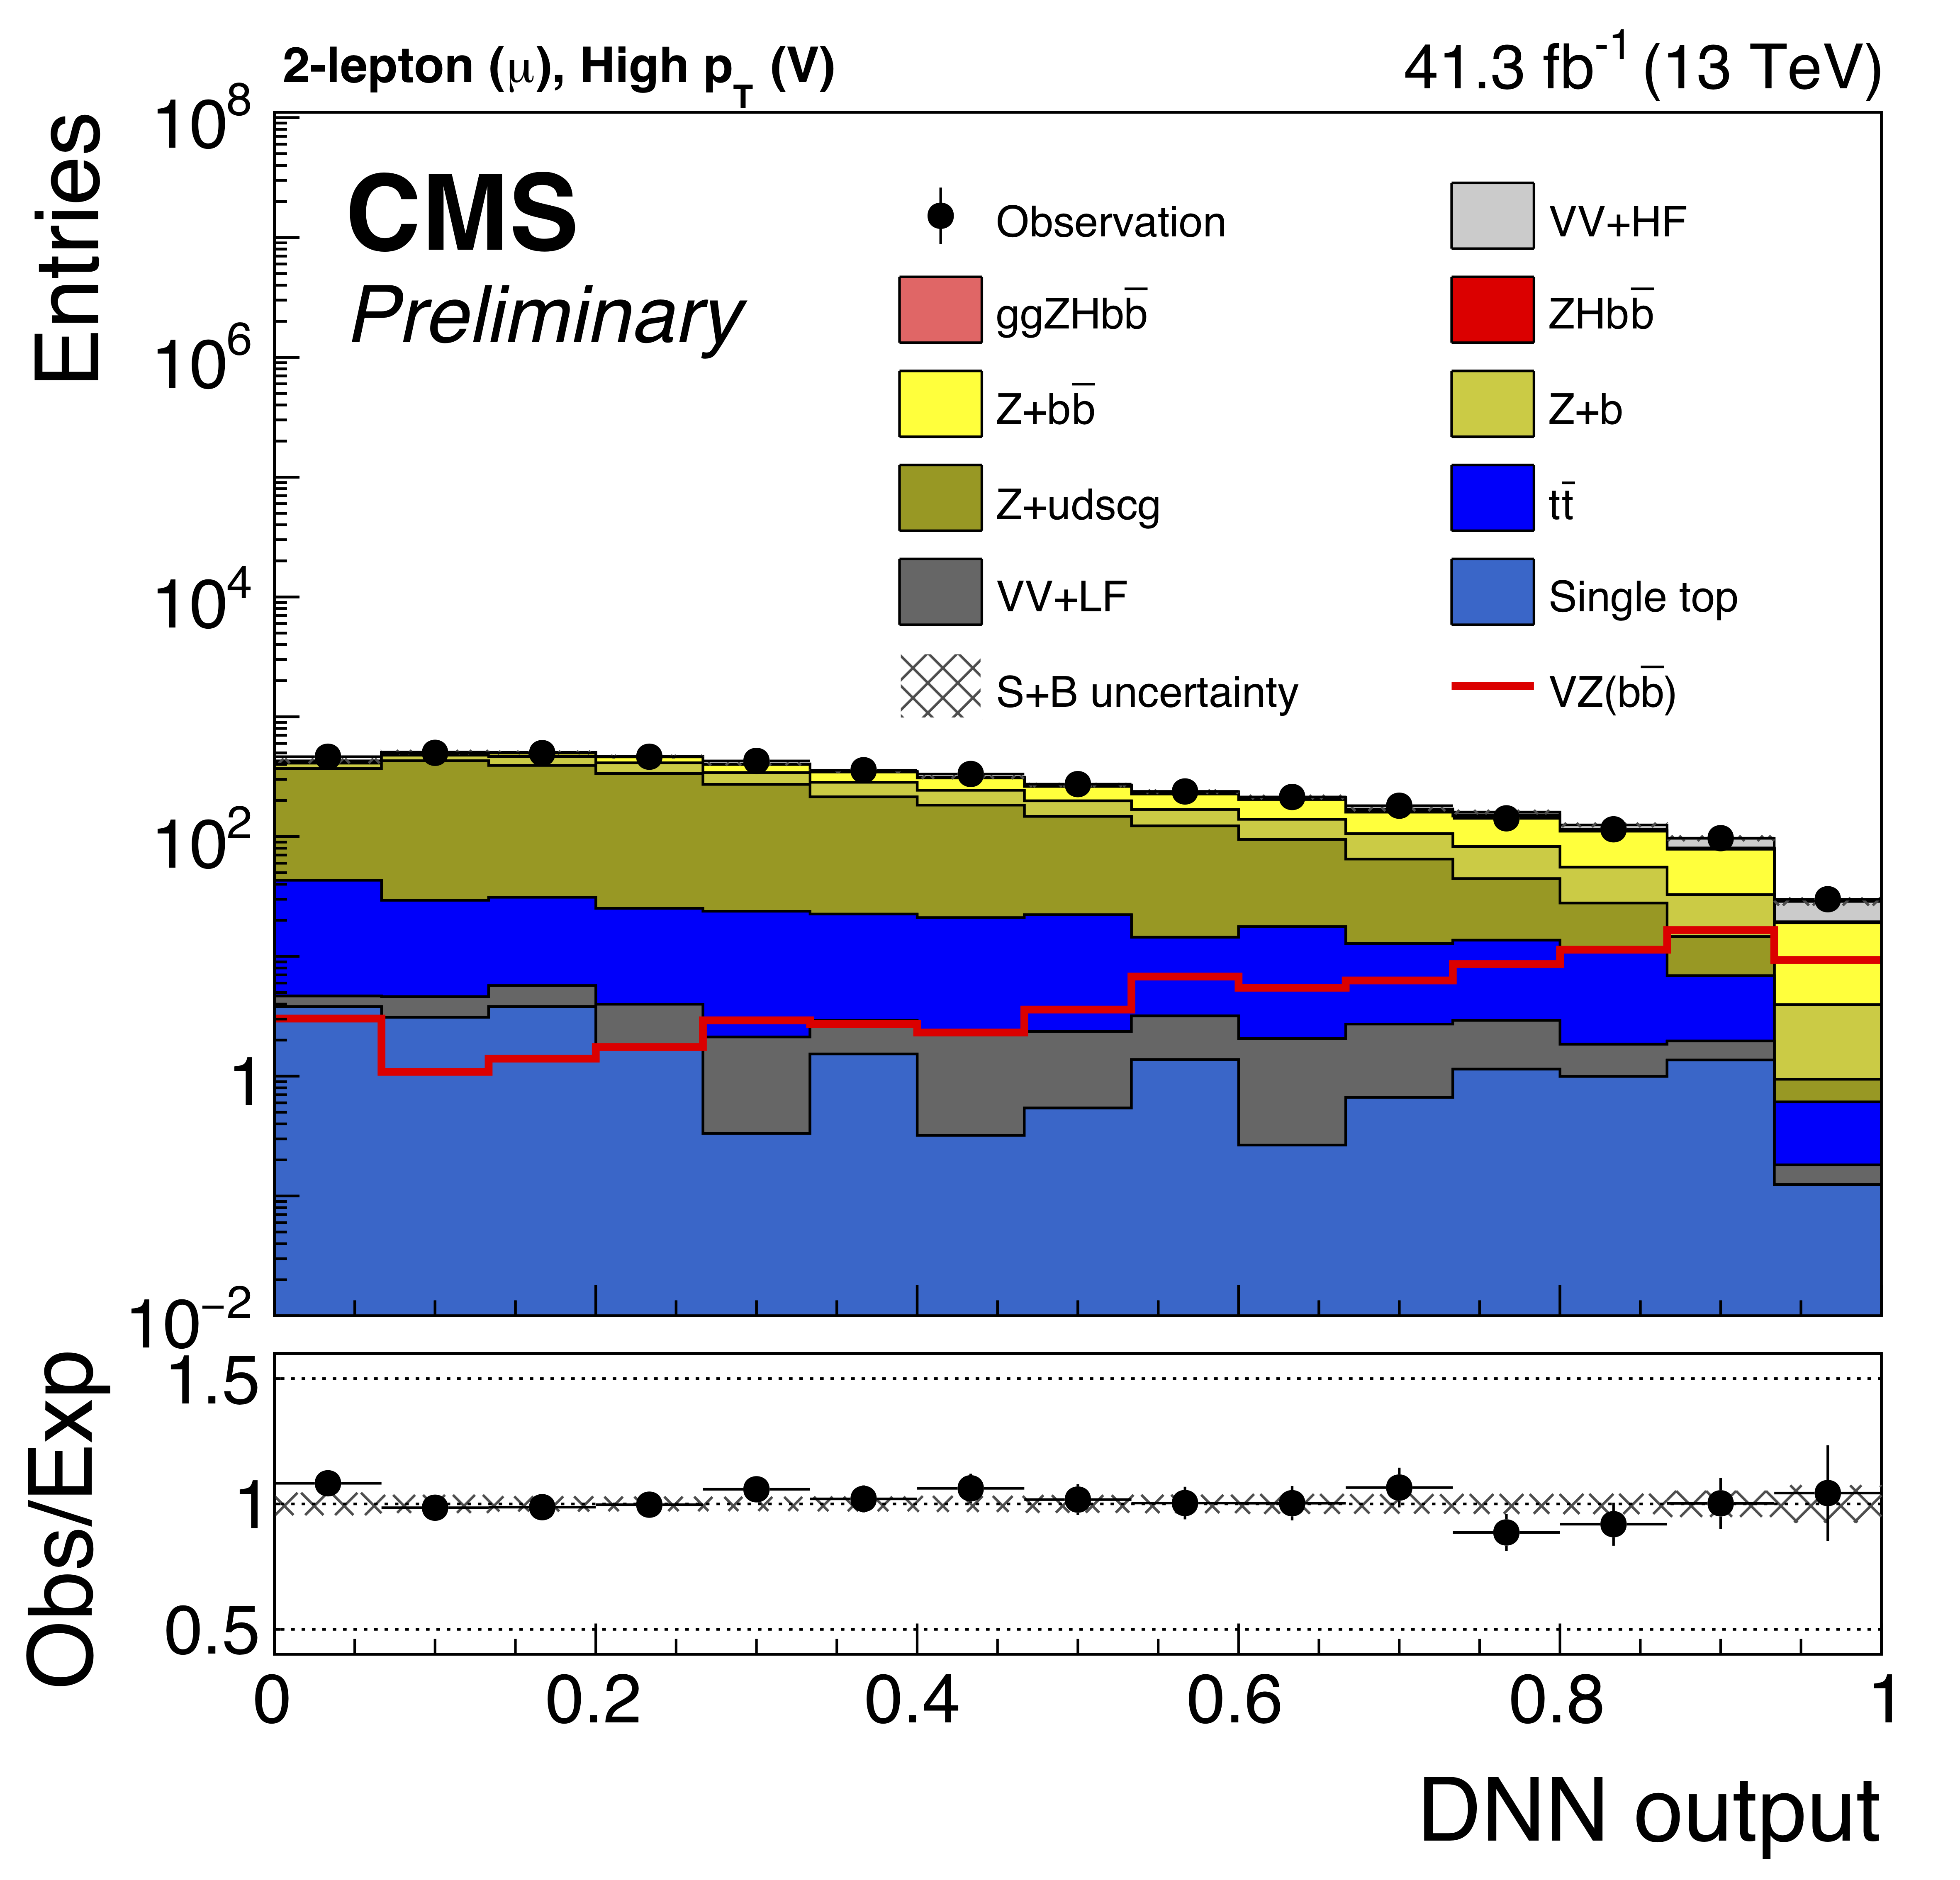
\includegraphics[width=0.285\linewidth]{images/SR_VZbb/vhbb_Zmm_1_13TeV2017_shapes_postfit_logy}} \qquad
  }
  \mbox{
    \subfigure [] {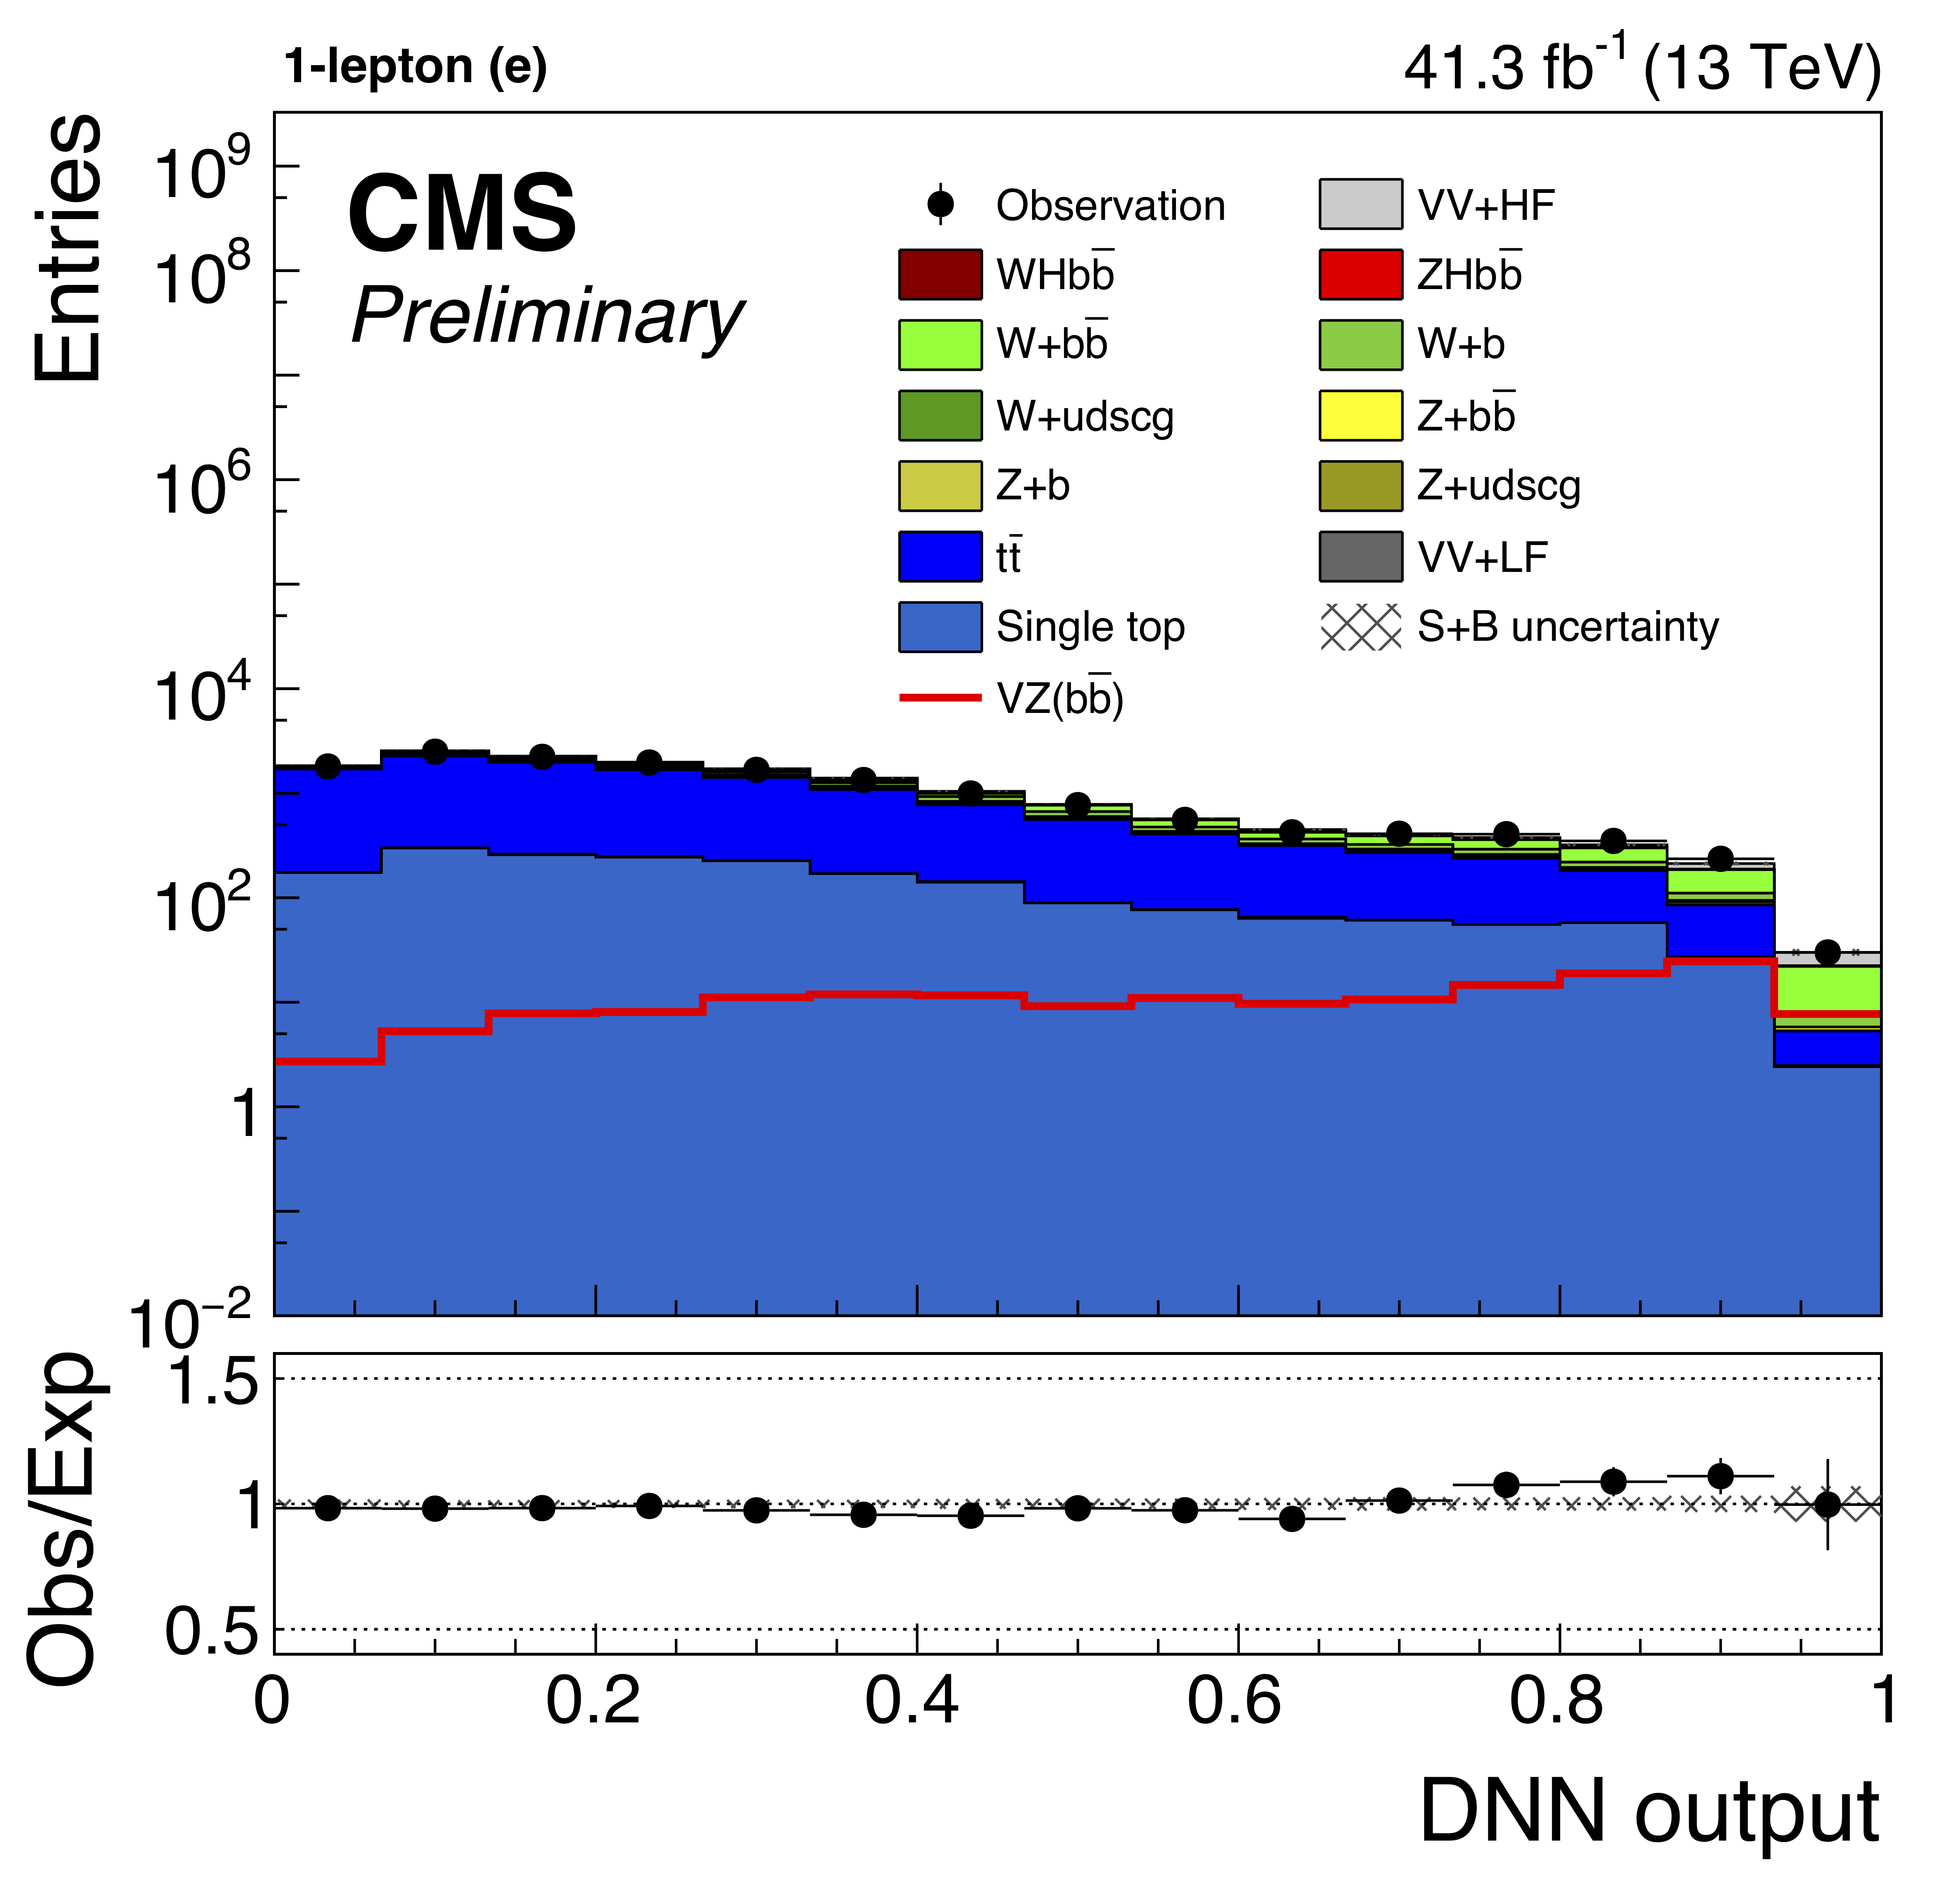
\includegraphics[width=0.285\linewidth]{images/SR_VZbb/vhbb_Wen_1_13TeV2017_shapes_postfit_logy}} \qquad
    \subfigure [] {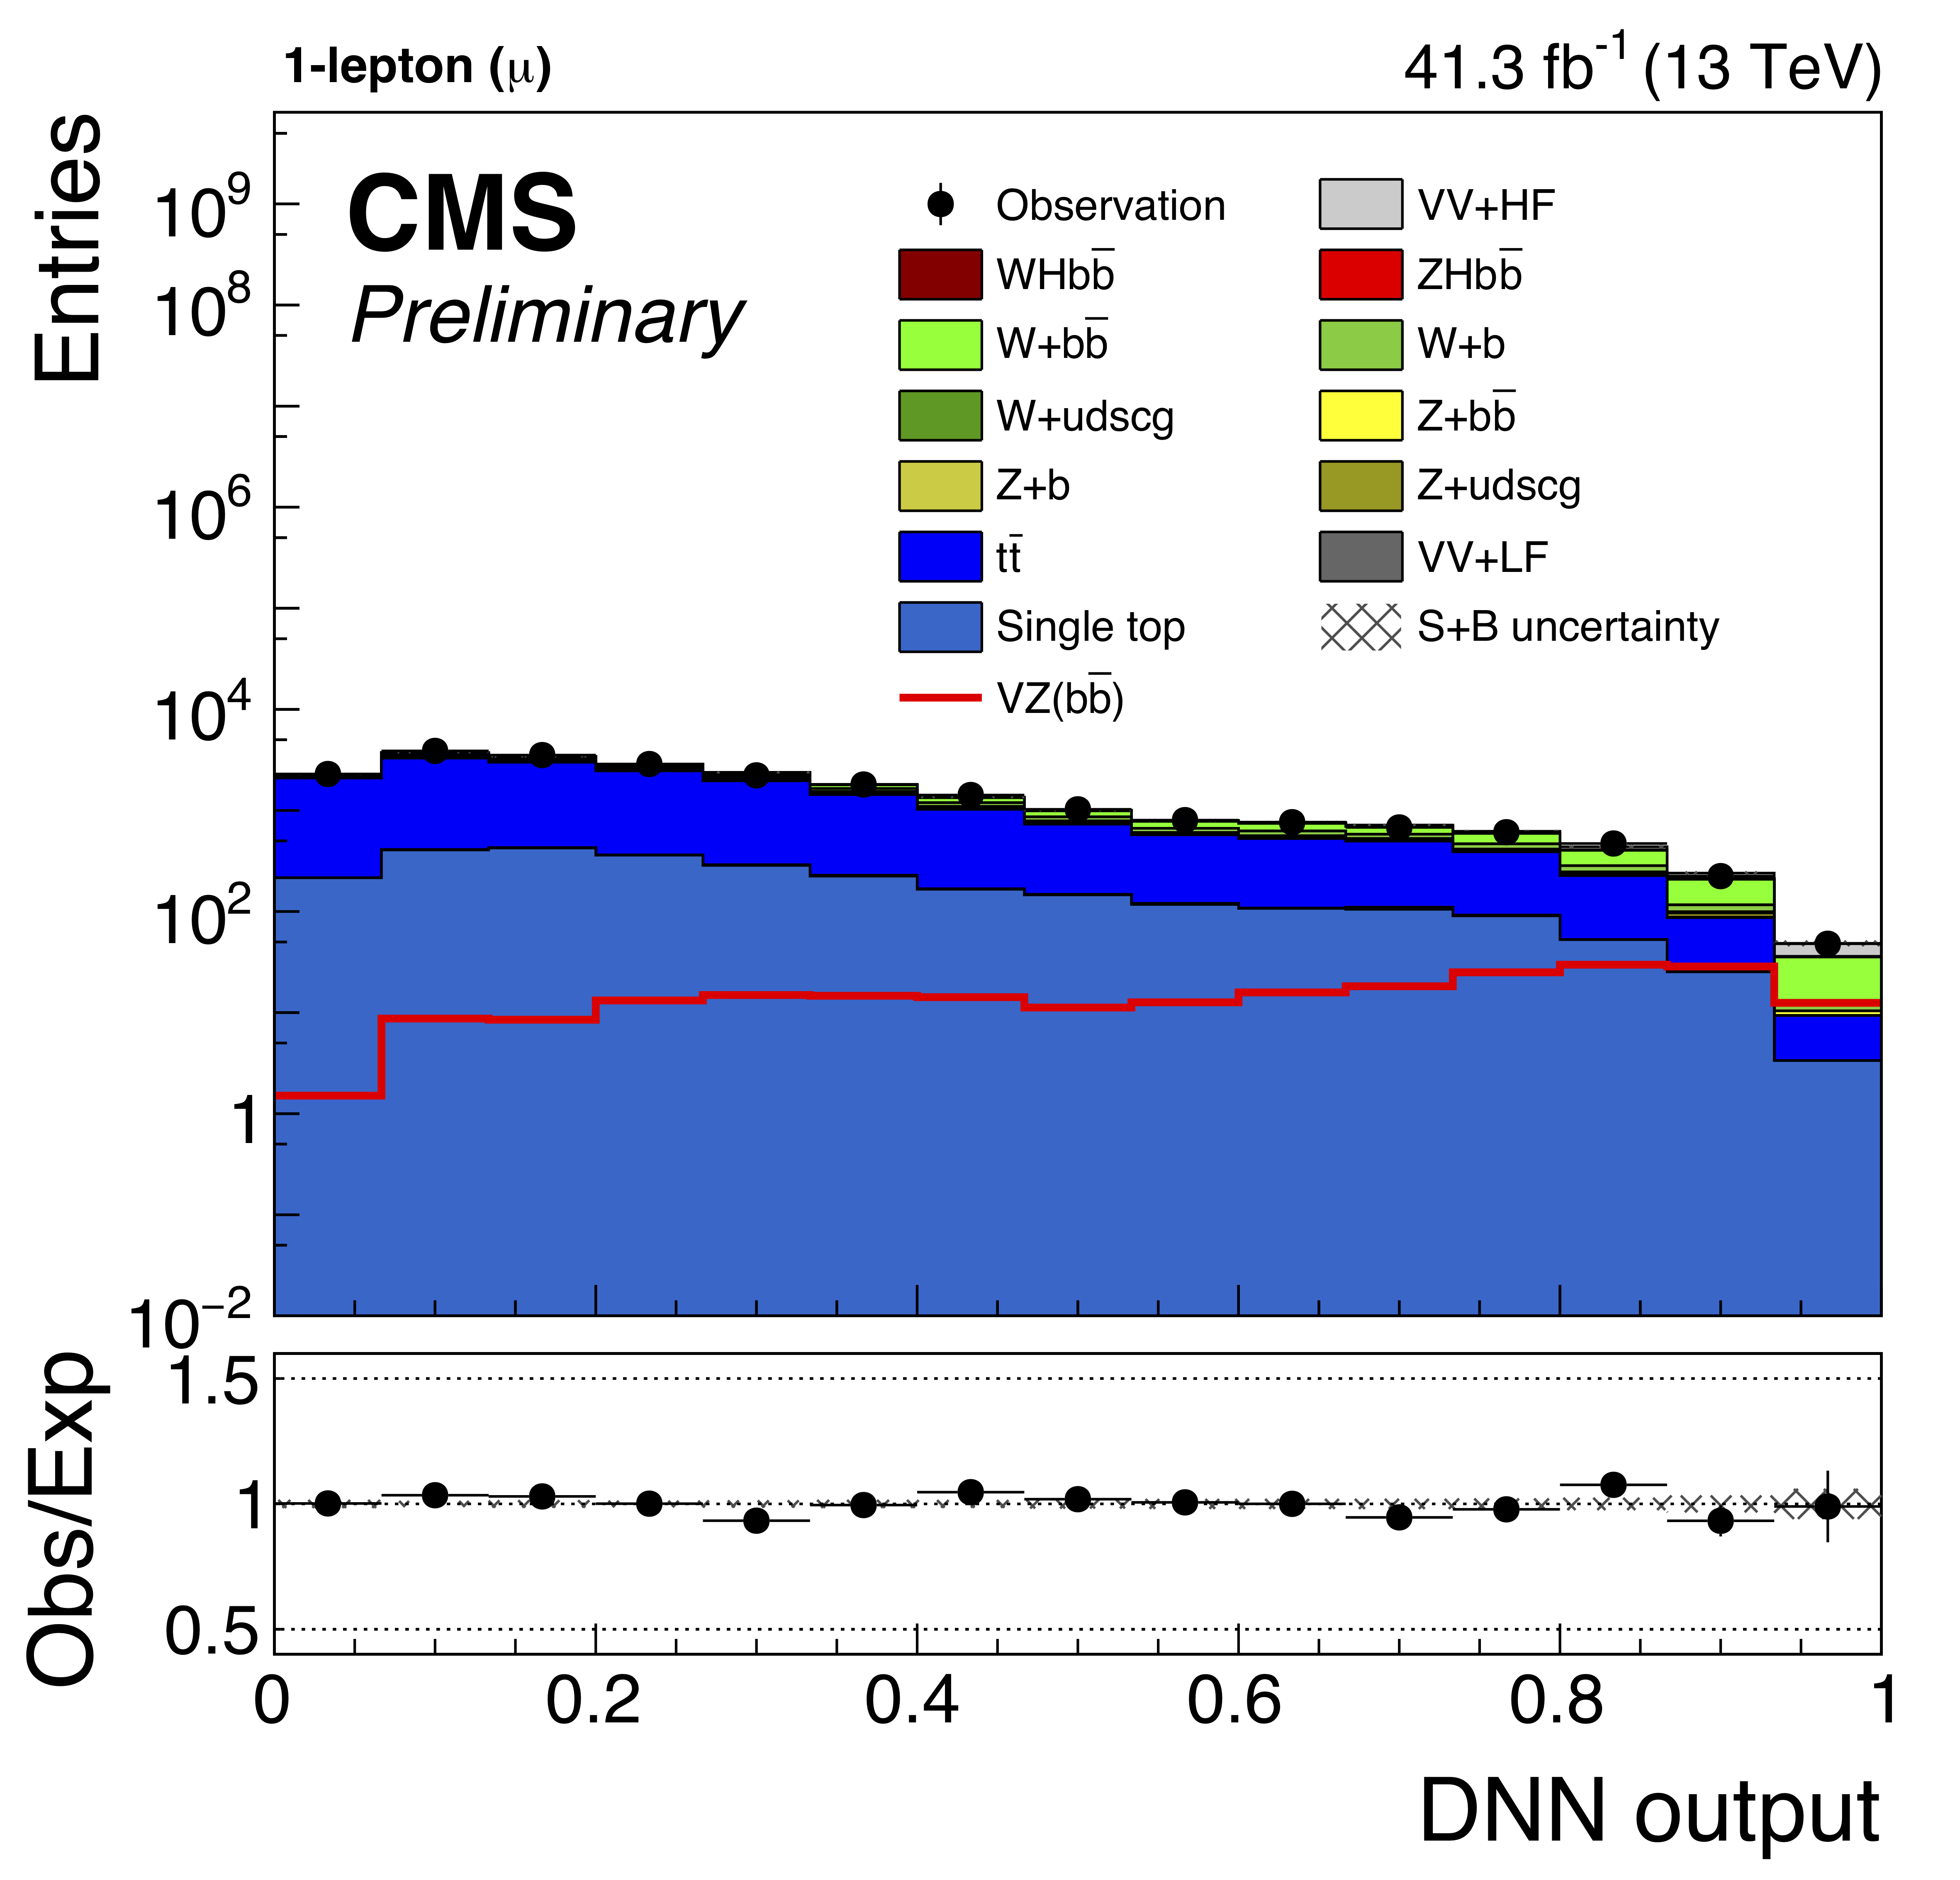
\includegraphics[width=0.285\linewidth]{images/SR_VZbb/vhbb_Wmn_1_13TeV2017_shapes_postfit_logy}} \qquad
  }
  \mbox{
    \subfigure [] {\includegraphics[width=0.285\linewidth]{images/SR_VZbb/vhbb_Znn_1_13TeV2017_shapes_postfit_logy}}
  }
  \caption[\VZbb\ Signal Region Distributions]{The post-fit \VZbb\ multivariate discriminant distributions of the A) low \pT(\bosV) \ZeeH; B) low \pT(\bosV) \ZmmH; C) high \pT(\bosV) \ZeeH; D) high \pT(\bosV) \ZmmH; E) \WenH; F) \WmnH; and G) \ZnnH\ channels.}
  \label{fig:SRVZbb}
\end{figure}

\begin{figure}[htbp]
  \centering
    \includegraphics[width=3.5in]{images/CMS-HIG-18-016_Figure-aux_009}
    \caption[\VZbb\ Combined Signal Region Distribution]{The post-fit multivariate discriminant distributions of signal, background, and data event yields combined for all \VZbb\ channels and sorted into bins of similar signal-to-background ratio. The \VZbb\ signal contribution (red) has been stacked above the sum of all background yields (gray). The bottom panel shows the data to background ratio (black points) and the sum of signal and background contributions divided by the background yield (red line).}
    \label{fig:SBVZbb}
\end{figure}

\begin{figure}[htbp]
  \centering
    \includegraphics[width=3.5in]{images/MuVZbb}
    \caption[\VZbb\ Analysis Signal Strengths]{The best fit signal strengths and their uncertainties for each of the channels of the \VZbb\ cross-check analysis.}
    \label{fig:MuVZbb}
\end{figure}

\section{Dijet Invariant Mass Analysis}

The optimal massless DNN score values that divide the signal regions of each of the decay channels into four separate mass categories are listed in Table \ref{tbl:MjjVHbb}. The data to MC scale factors obtained by the maximum likelihood fit are shown in Table \ref{tbl:SFMjj}. The expected post-fit significance of the excess over the background prediction is $2.19\sigma$, while the observed significance is $1.33\sigma$. The best fit signal strength is $\mu = 0.59_{-0.45}^{+0.45}$ for all channels combined. By combining the dijet invariant mass distributions of all channels with weight $S/(S+B)$, where $S$ is the post-fit \VHbb signal yield and $B$ is the post-fit total background yield specific to each channel, and then subtracting the contributions of all background processes except for \VZbb, the capability of resolving the \VHbb\ mass peak against the \VZbb\ mass peak without a multivariate analysis is shown in Figure \ref{fig:WeightedMjj}.

\begin{table}[htbp]
  \caption[Dijet Invariant Mass Analysis Categories]{The massless DNN scores which define the boundaries of the four dijet invariant mass categories of each \VHbb\ channel.}
  \label{tbl:MjjVHbb}
  \begin{tabularx}{6.5in}{XX}
    \hline
    Channel                & Mass Category Boundaries          \\
    \hline
    \ZnnH                  & [0.00, 0.558, 0.768, 0.838, 1.00] \\
    \WlnH                  & [0.00, 0.550, 0.856, 0.941, 1.00] \\
    \ZllH, Low \pT(\bosV)  & [0.00, 0.662, 0.875, 0.927, 1.00] \\
    \ZllH, High \pT(\bosV) & [0.00, 0.486, 0.836, 0.899, 1.00] \\
    \hline
  \end{tabularx}
\end{table}

\begin{table}[htbp]
  \caption[Dijet Invariant Mass Analysis Scale Factors]{The data to Monte-Carlo scale factors obtained by the simultaneous maximum likelihood fit over all \VHbb\ channels for the dijet invariant mass analysis. The errors include both statistical and systematic uncertainties.}
  \label{tbl:SFMjj}
  \begin{tabularx}{6.5in}{lXXll}
    \hline
    Process       & \ZnnH           & \WlnH           & \ZllH, Low \pT(\bosV) & \ZllH, High \pT(\bosV) \\
    \hline
    \Wlight       & $1.02 \pm 0.07$ & $1.02 \pm 0.07$ & -                     & -                      \\
    \Wb           & $1.82 \pm 0.14$ & $1.82 \pm 0.14$ & -                     & -                      \\
    \Wbb          & $2.05 \pm 0.22$ & $2.05 \pm 0.22$ & -                     & -                      \\
    \Zlight       & $0.95 \pm 0.08$ & -               & $0.88 \pm 0.06$       & $0.81 \pm 0.05$        \\
    \Zb           & $1.16 \pm 0.16$ & -               & $0.99 \pm 0.13$       & $1.12 \pm 0.11$        \\
    \Zbb          & $1.00 \pm 0.08$ & -               & $0.72 \pm 0.06$       & $0.82 \pm 0.07$        \\
    \qrkt\qrktbar & $0.97 \pm 0.08$ & $0.90 \pm 0.07$ & $0.89 \pm 0.07$       & $0.88 \pm 0.07$        \\
    \hline
  \end{tabularx}
\end{table}

\begin{figure}[htbp]
  \centering
    \includegraphics[width=3.5in]{images/only2017_shapesMjj1617_postfit}
    \caption[Combined Dijet Invariant Mass Distribution]{The dijet invariant mass distribution for events weighted by $S/(S+B)$ in all channels combined. The data (black) and the fitted \VHbb\ signal (red) and \VZbb\ background (gray) distributions are shown with all other fitted backgrounds subtracted. The vertical error bars represent the $1\sigma$ statistical uncertainty on the data before background subtraction, while the blue error band represents the $1\sigma$ total uncertainty on the signal and all background processes.}
    \label{fig:WeightedMjj}
\end{figure}

\section{\VHbb\ Analysis}

The data to MC scale factors obtained by the maximum likelihood fit are shown in Table \ref{tbl:SFVHbb} and show good agreement with those obtained by the \VZbb\ cross-check analysis. The post-fit multivariate discriminant distributions of each channel are shown individually in Figure \ref{fig:SRVHbb} and combined in Figure \ref{fig:SBVHbb}. The expected post-fit significance of the excess over the background prediction is $3.1\sigma$, while the observed significance is $3.3\sigma$. The best fit signal strength is $\mu = 1.08_{-0.33}^{+0.35}$ for all channels combined and the signal strengths of the individual channels, shown in Figure \ref{fig:MuVHbb}, are compatible with a $p$-value of 96\%. These results reestablish evidence for the \VHbb\ decay. The contributions of the major uncertainty sources are listed in Table \ref{tbl:UncVHbb} and decomposed into four groups: theory, size of simulated samples, experimental, and statistical. For each major source of uncertainty, the largest individual subcomponents are also listed.

\begin{table}[htbp]
  \caption[\VHbb\ Analysis Scale Factors]{The data to Monte-Carlo scale factors obtained by the simultaneous maximum likelihood fit over all \VHbb\ channels. The errors include both statistical and systematic uncertainties.}
  \label{tbl:SFVHbb}
  \begin{tabularx}{6.5in}{lXXll}
    \hline
    Process       & \ZnnH           & \WlnH           & \ZllH, Low \pT(\bosV) & \ZllH, High \pT(\bosV) \\
    \hline
    \Wlight       & $1.04 \pm 0.07$ & $1.04 \pm 0.07$ & -                     & -                      \\
    \Wb           & $2.09 \pm 0.16$ & $2.09 \pm 0.16$ & -                     & -                      \\
    \Wbb          & $1.74 \pm 0.21$ & $1.74 \pm 0.21$ & -                     & -                      \\
    \Zlight       & $0.95 \pm 0.09$ & -               & $0.89 \pm 0.06$       & $0.81 \pm 0.05$        \\
    \Zb           & $1.02 \pm 0.17$ & -               & $0.94 \pm 0.12$       & $1.17 \pm 0.10$        \\
    \Zbb          & $1.20 \pm 0.11$ & -               & $0.81 \pm 0.07$       & $0.88 \pm 0.08$        \\
    \qrkt\qrktbar & $0.99 \pm 0.07$ & $0.93 \pm 0.07$ & $0.89 \pm 0.07$       & $0.91 \pm 0.07$        \\
    \hline
  \end{tabularx}
\end{table}

\begin{figure}[htbp]
  \centering
  \mbox{
    \subfigure [] {\includegraphics[width=0.285\linewidth]{images/SR_VHbb/CMS-HIG-18-016_Figure-aux_007-d}} \qquad
    \subfigure [] {\includegraphics[width=0.285\linewidth]{images/SR_VHbb/CMS-HIG-18-016_Figure-aux_007-c}} \qquad
  }
  \mbox{
    \subfigure [] {\includegraphics[width=0.285\linewidth]{images/SR_VHbb/CMS-HIG-18-016_Figure-aux_007-b}} \qquad
    \subfigure [] {\includegraphics[width=0.285\linewidth]{images/SR_VHbb/CMS-HIG-18-016_Figure-aux_007-a}} \qquad
  }
  \mbox{
    \subfigure [] {\includegraphics[width=0.285\linewidth]{images/SR_VHbb/CMS-HIG-18-016_Figure-aux_007-f}} \qquad
    \subfigure [] {\includegraphics[width=0.285\linewidth]{images/SR_VHbb/CMS-HIG-18-016_Figure-aux_007-e}} \qquad
  }
  \mbox{
    \subfigure [] {\includegraphics[width=0.285\linewidth]{images/SR_VHbb/CMS-HIG-18-016_Figure-aux_007-g}}
  }
  \caption[\VHbb\ Signal Region Distributions]{The post-fit \VHbb\ multivariate discriminant distributions of the A) low \pT(\bosV) \ZeeH; B) low \pT(\bosV) \ZmmH; C) high \pT(\bosV) \ZeeH; D) high \pT(\bosV) \ZmmH; E) \WenH; F) \WmnH; and G) \ZnnH\ channels.}
  \label{fig:SRVHbb}
\end{figure}

\begin{figure}[htbp]
  \centering
    \includegraphics[width=3.5in]{images/CMS-HIG-18-016_Figure-aux_008-a}
    \caption[\VHbb\ Combined Signal Region Distribution]{The post-fit multivariate discriminant distributions of signal, background, and data event yields combined for all \VHbb\ channels and sorted into bins of similar signal-to-background ratio. The \VHbb\ signal contribution (red) has been stacked above the sum of all background yields (gray). The bottom panel shows the data to background ratio (black points) and the sum of signal and background contributions divided by the background yield (red line).}
    \label{fig:SBVHbb}
\end{figure}

\begin{figure}[htbp]
  \centering
    \includegraphics[width=3.5in]{images/MuVHbb}
    \caption[\VHbb\ Analysis Signal Strengths]{The best fit signal strengths and their uncertainties for each of the channels of the \VHbb\ analysis.}
    \label{fig:MuVHbb}
\end{figure}

\begin{table}[htbp]
  \caption[\VHbb\ Main Uncertainty Sources]{The contributions of the main uncertainty sources in the measurement of the \VHbb\ signal strength. Due to correlations between the nuisance parameters of different sources in the maximum likelihood fit, the sum in quadrature of each source is not necessarily the total uncertainty of each major component.}
  \label{tbl:UncVHbb}
  \begin{tabularx}{6.5in}{Xcc}
    \hline
    Uncertainty Source                        & \multicolumn{2}{c}{$\Delta\mu$} \\
    \hline
    Theory                                    & $+0.11$        & $-0.09$        \\
    - Signal theory                           & $+0.07$        & $-0.04$        \\
    - Background theory                       & $+0.08$        & $-0.08$        \\
    Size of simulated samples                 & $+0.12$        & $-0.12$        \\
    Experimental                              & $+0.16$        & $-0.15$        \\
    - Luminosity                              & $+0.03$        & $-0.03$        \\
    - Lepton efficiency                       & $+0.02$        & $-0.01$        \\
    - Jet energy scale and resolution         & $+0.05$        & $-0.05$        \\
    - \qrkb-Tagging efficiency                & $+0.09$        & $-0.08$        \\
    - Other experimental uncertainties        & $+0.10$        & $-0.09$        \\
    Statistical                               & $+0.26$        & $-0.26$        \\
    - Background control region normalization & $+0.12$        & $-0.12$        \\
    Total                                     & $+0.35$        & $-0.33$        \\
    \hline
  \end{tabularx}
\end{table}

\section{Combinations with Past CMS Results}

A combination of the 2017 \VHbb\ analysis results with those of the 2016 \VHbb\ analysis published in Ref. \cite{CMSVHbbEvidence} increases the expected and observed significance to $4.16\sigma$ and $4.36\sigma$, respectively, with a best fit signal strength of $\mu = 1.06_{-0.26}^{+0.25}$. A further combination of these analyses with the Run 1 analysis published in Ref. \cite{CMSVHbbRun1} further increases the expected and observed significance to $4.88\sigma$ and $4.82\sigma$, respectively, with a best fit signal strength of $\mu = 1.01_{-0.23}^{+0.22}$. The results of this combination fall short of establishing an observation of the \VHbb\ decay.

A global fit is performed that combines all available CMS analyses of different \Htobb\ production processes, including this analysis of \VHbb, gluon fusion\cite{ggHbb}, vector boson fusion\cite{VBF}, and \qrkt\qrktbar\ associated production\cite{CMSttH1,CMSttH2,CMSttH3}. Because the results of these analyses span multiple datasets collected at 7, 8, and 13 \TeV\ and different detector operating conditions, most systematic uncertainty sources are treated as uncorrelated. For analyses using the same collision energies, the jet energy scale uncertainties are treated as correlated between those processes. The theoretical uncertainties are correlated between all processes and datasets. This grand combination achieves an expected and observed significance of $5.5\sigma$ and $5.6\sigma$, respectively. The best fit signal strength is $\mu = 1.04 \pm 0.20$, and the signal strengths of the different \Htobb\ production modes are shown in Figure \ref{fig:MuHbb}. This marks the first observation of the \Htobb\ decay at the CMS experiment and the measured signal strength indicates agreement with the Standard Model expectation.

\begin{figure}[htbp]
  \centering
    \includegraphics[width=3.5in]{images/CMS-HIG-18-016_Figure_003}
    \caption[\Hbb\ Combination Signal Strengths]{The best fit signal strengths and their uncertainties for each of the analyses of the different \Htobb\ production modes that participated in the grand combination.}
    \label{fig:MuHbb}
\end{figure}
  %These chapters are not included in the template
%\chapter{CONCLUSIONS} \label{conclusions}

A search for the Standard Model Higgs boson produced in association with a weak vector boson and decaying into a bottom-antibottom quark pair (\bb) has been presented for the \VHbb\ decay channels \ZnnHbb, \WenHbb, \WmnHbb, \ZeeHbb, and \ZmmHbb. The search is performed with a dataset corresponding to an integrated luminosity of 41.3 \invfb\ at a center-of-mass energy of $\sqrt{s} = 13\ \TeV$ recorded by the CMS experiment at the LHC during Run 2 in 2017. An excess of events in data over the expected background is observed with a significance of 3.3 standard deviations, as compared to an expected significance of 3.1 standard deviations under the Standard Model prediction for a Higgs boson of mass \massH\ = 125.09 \GeV decaying to bottom quarks. The corresponding signal strength of this excess relative to the Standard Model Higgs boson is measured to be $\mu = 1.08_{-0.33}^{+0.35}$, which suggests compatibility with the Standard Model.

A grand combination of this result is performed with previous measurements made by the CMS collaboration of the associated vector boson, gluon fusion, vector boson fusion, and associated top quark production modes for \Htobb. This combination achieves an observed significance of 5.6 standard deviations, with an expected significance of 5.5 standard deviations, and measures an overall signal strength of $\mu = 1.04 \pm 0.20$ for the \Htobb\ decay. This constitutes the observation of the \Htobb\ decay by the CMS collaboration, with no clear indication of physics beyond the Standard Model.

Although the \Htobb\ decay has been observed, the continued study of this decay offers an opportunity to check for anomalous Higgs' Yukawa couplings and, given it has the largest branching fraction of all Higgs' decays, to improve the constraints placed on the total decay width of the Higgs boson. The focus of future analyses will then prioritize improving the precision of the measurement of the \VHbb\ production cross section and the \Htobb\ branching fraction. By refining the strategy adopted for the dijet invariant mass analysis, where a multivariate classifier is evaluated in such a way that its output is decorrelated from the fitted distribution, the effects of shape systematics could be reduced as the dijet invariant mass distributions of the background processes are typically flat. Similar techniques that warrant further investigation include a method of rescaling the input features to decorrelate a multivariate classifier from specific variables that has been successfully used by the \Htomm\ analysis\cite{HTOMUMU} and an adversarial training method that has been proposed to decorrelate jet tagging algorithms from the jet mass\cite{ADVTRAIN}.

Future analyses of the \VHbb\ decay into Run 3 and beyond face increased luminosities which may cause the dijet invariant mass resolution and \qrkb-tagging performance to degrade due to increased pileup. More robust methods of pileup removal such as the pileup per particle identification (PUPPI)\cite{PUPPI} algorithm may be required under these harsher conditions. Future analyses performed at higher center-of-mass energies may also benefit from a dedicated jet substructure\cite{JETSUB} analysis, given that the bottom quarks from the Higgs decay become highly collimated at very high boosts. While typical jet algorithms may be unable to resolve the merged \qrkb-jets, jet substructure techniques such as those used by the search for \Htobb\ using the gluon fusion production mode\cite{ggHbb} are capable of identifying jet constituents and their flavor. Novel applications of machine learning in the field of high energy physics towards jet flavor tagging, such as the DeepJet\cite{DEEPJET} algorithm, and discovery significance optimization\cite{OPTSIG} may improve the sensitivity of the analysis.


%-----------------------------------------------------------------------%

% Use the appropriate file depending upon the number of appendices you have


% The Editorial Office Requirements for the Table of Contents cause a significant problem
%in Latex if there is only one Appendix. The Appendix is no longer labeled "A" in the TOC
%but has the word "APPENDIX" placed in front of the title of the Appendix. This can be done
%without issue IF nothing needs to be numbered by LaTeX in the Appendix. Unfortunately, most of the time
%something needs to be numbered in that single Appendix. For this reason we have included the IFTHENELSE switch
%found in this document and at the beginning of AppendixA. We assume that if you have any appendices, that you have more than one. However, you DO only have one appendix DO NOT USE THIS FILE!!!!!!!!!!!!!!!!!!!!!!!
%
% OneSingleAppendix.tex has all the settings needed to adjust for a single appendix
% you will have a major problem with your TOC if you use this file with a single appendix!!!!!

%
% Comment (or delete) all of the \input{AppendixB} commands except those you are using.
%Then open the AppendixA.tex file and continue there.

%you can add/substract individual appendices through by using the /include{appendix'X'}
% and creating/deleting the appropriate files
\appendix %
%\clearpage%

\addtocontents{toc}{\protect\addvspace{10pt}\noindent{APPENDIX} \protect\hfill\par}{}
\setcounter{equation}{0}

% % % % % % % If you have a single appendix, you should be using OneSingleAppendix.tex
% % % % % % % NOT this file

\chapter{EVENT DISPLAYS}

Collision events recorded by the CMS detector can be visualized as event displays using the Fireworks application developed by the CMS collaboration.\cite{Fireworks} Event displays are used to visually summarize particle interactions with the detector's subsystems by rendering reconstructed objects of interest such as particle tracks and jets over a 3D model of the detector. Figures \ref{fig:evt_disp_Znn} through \ref{fig:evt_disp_Zmm} each show multiple different perspectives of an event display for a candidate signal region event from each decay channel. The candidate events were chosen based on their high DNN scores, which indicate that the DNN of their corresponding decay channel classified them as a signal event with high confidence. Although the event metadata are provided on the event displays, other event-level quantities of interest are shown in Table \ref{tbl:event_display}.

\begin{table}[htbp]
  \caption[Event Display Candidate Information]{Information for the candidate signal region events visualized by the event display. The values of the kinematic quantities are reported in units of \GeV\ and the \btag\ algorithm is DeepCSV.}
  \label{tbl:event_display}
  \begin{tabularx}{6.5in}{XXXrrXXXX}
    \hline
    Channel & \mjj   & \pTjj  & \pTjmax & \pTjmin & \btagmax & \btagmin & \pTV   & DNN score \\
    \hline
    \Znn    & 121.56 & 319.43 & 195.99  & 129.81  & 0.999    & 0.993    & 319.10 & 0.975     \\
    \Wen    & 126.49 & 259.66 & 179.31  & 87.31   & 0.999    & 0.995    & 295.75 & 0.989     \\
    \Wmn    & 117.69 & 250.55 & 177.33  & 85.28   & 0.996    & 0.995    & 259.80 & 0.993     \\
    \Zee    & 114.14 & 286.17 & 216.54  & 97.82   & 0.990    & 0.957    & 311.33 & 1.00      \\
    \Zmm    & 111.39 & 100.12 & 78.66   & 69.53   & 0.984    & 0.975    & 466.83 & 1.00      \\
    \hline
  \end{tabularx}
\end{table}

For each figure, the perspective of the largest subfigure is a projection of the event display onto the \textit{xz}-plane, unless otherwise specified. The perspective of both of the smaller subfigures is a projection of the event display onto the \textit{xy}-plane, with the subfigure on the right zoomed in on the interaction point. This level of zoom is necessary to show the secondary vertices and their associated tracks, shown in black, and to appreciate that those tracks do not extrapolate well to any of the primary vertices, shown in yellow.

\begin{figure}[htbp]
  \centering
  \mbox{
    \subfigure [] {\includegraphics[width=\linewidth]{images/Znn_PerspXOZ_w}}
  }
  \mbox{
    \subfigure [] {\includegraphics[width=0.5\linewidth]{images/Znn_rhophi_w}}
    \subfigure [] {\includegraphics[width=0.5\linewidth]{images/ZnnSV_rhophi_w}}
  }
  \caption[Event Display for \ZnnHbb\ Candidate]{The event display for a candidate \ZnnHbb\ event A) from a 3D perspective view; B) projected onto the \textit{xy}-plane; and C) projected onto the \textit{xy}-plane and zoomed in on the interaction point. The purple arrow represents the missing transverse momentum from the invisible leptonic decay of the \bosZ\ boson while the two yellow cones with their blue and red calorimeter towers represent the two \qrkb-jets from the decay of the Higgs boson. The secondary vertices of the \qrkb-jets and their associated tracks (black) are visible in C.}
  \label{fig:evt_disp_Znn}
\end{figure}

\begin{figure}[htbp]
  \centering
  \mbox{
    \subfigure [] {\includegraphics[width=\linewidth]{images/Wen_rhoz_w}}
  }
  \mbox{
    \subfigure [] {\includegraphics[width=0.5\linewidth]{images/Wen_rhophi_w}}
    \subfigure [] {\includegraphics[width=0.5\linewidth]{images/WenSV_rhophi_w}}
  }
  \caption[Event Display for \WenHbb\ Candidate]{The event display for a candidate \WenHbb\ event A) projected onto the \textit{xz}-plane; B) projected onto the \textit{xy}-plane; and C) projected onto the \textit{xy}-plane and zoomed in on the interaction point. The cyan track leading to a red calorimeter tower and the purple arrow represent the electron and the missing transverse momentum from the leptonic decay of the \bosW\ boson, respectively, while the two yellow cones with their blue and red calorimeter towers represent the two \qrkb-jets from the decay of the Higgs boson. The secondary vertices of the \qrkb-jets and their associated tracks (black) are visible in C. The red track associated with one of the \qrkb-jets is likely a muon resulting from a semi-leptonic decay of the \qrkb-hadron.}
  \label{fig:evt_disp_Wen}
\end{figure}

\begin{figure}[htbp]
  \centering
  \mbox{
    \subfigure [] {\includegraphics[width=\linewidth]{images/Wmn_rhoz_w}}
  }
  \mbox{
    \subfigure [] {\includegraphics[width=0.5\linewidth]{images/Wmn_rhophi_w}}
    \subfigure [] {\includegraphics[width=0.5\linewidth]{images/WmnSV_rhophi_w}}
  }
  \caption[Event Display for \WmnHbb\ Candidate]{The event display for a candidate \WmnHbb\ event A) projected onto the \textit{xz}-plane; B) projected onto the \textit{xy}-plane; and C) projected onto the \textit{xy}-plane and zoomed onto the interaction point. The red track and the purple arrow represent the muon and the missing transverse momentum from the leptonic decay of the \bosW\ boson, respectively, while the two yellow cones with their blue and red calorimeter towers represent the two \qrkb-jets from the decay of the Higgs boson. The secondary vertices of the \qrkb-jets and their associated tracks (black) are visible in C.}
  \label{fig:evt_disp_Wmn}
\end{figure}

\begin{figure}[htbp]
  \centering
  \mbox{
    \subfigure [] {\includegraphics[width=\linewidth]{images/Zee_rhoz_w}}
  }
  \mbox{
    \subfigure [] {\includegraphics[width=0.5\linewidth]{images/Zee_rhophi_w}}
    \subfigure [] {\includegraphics[width=0.5\linewidth]{images/ZeeSV_rhophi_w}}
  }
  \caption[Event Display for \ZeeHbb\ Candidate]{The event display for a candidate \ZeeHbb\ event A) projected onto the \textit{xz}-plane; B) projected onto the \textit{xy}-plane; and C) projected onto the \textit{xy}-plane and zoomed onto the interaction point. The cyan tracks leading to red calorimeter towers represent the electrons from the leptonic decay of the \bosZ\ boson, while the two yellow cones with their blue and red calorimeter towers represent the two \qrkb-jets from the decay of the Higgs boson. The secondary vertices of the \qrkb-jets and their associated tracks (black) are visible in C. The low missing transverse momentum close in azimuthal angle to one of the \qrkb-jets is suggestive of jet energy mismeasurement. This may be related to the blue calorimeter tower without obvious associated tracks, which may have resulted from the decay of a neutral hadron.}
  \label{fig:evt_disp_Zee}
\end{figure}

\begin{figure}[htbp]
  \centering
  \mbox{
    \subfigure [] {\includegraphics[width=\linewidth]{images/Zmm_rhoz_w}}
  }
  \mbox{
    \subfigure [] {\includegraphics[width=0.5\linewidth]{images/Zmm_rhophi_w}}
    \subfigure [] {\includegraphics[width=0.5\linewidth]{images/ZmmSV_rhophi_w}}
  }
  \caption[Event Display for \ZmmHbb\ Candidate]{The event display for a candidate \ZmmHbb\ event A) projected onto the \textit{xz}-plane; B) projected onto the \textit{xy}-plane; and C) projected onto the \textit{xy}-plane and zoomed onto the interaction point. The red tracks represent the muons from the leptonic decay of the \bosZ\ boson, while the two yellow cones with their blue and red calorimeter towers located opposite to the red tracks represent the two \qrkb-jets from the decay of the Higgs boson. The secondary vertices of the \qrkb-jets and their associated tracks (black) are visible in C. The two other yellow cones could represent jets caused by initial or final state radiation, neither of which were \qrkb-tagged.}
  \label{fig:evt_disp_Zmm}
\end{figure}

 %
%\chapter{AN EXAMPLE OF A HALF TITLE PAGE}%
\label{appendixB}

\clearpage %remove this command if your appendix doesn't start with a landscaped page!!!!!
\thispagestyle{plain}
\begin{landscape}
\begin{figure}

  \begin{center}
    \includegraphics[width=6in]{images/LaTeX2e_logo.eps}
    \caption{\LaTeX 2\ensuremath{\epsilon.} logo}\label{biglogo}
  \end{center}
\end{figure}
\end{landscape}


This is how a section should look if the first page is a landscape page.
Lorem ipsum dolor sit amet, consectetuer adipiscing elit. Ut sit
amet nulla. Integer mauris turpis, dapibus ac, auctor non, vehicula
sit amet, magna. Suspendisse eu tellus. Etiam porta. Donec magna.
Donec ut dui. In hac habitasse platea dictumst. Nullam suscipit, mi
at adipiscing commodo, lorem erat scelerisque erat, non pulvinar leo
mi eu metus. Phasellus id felis. Sed quam purus, molestie quis,
ultrices nec, dictum at, magna. Proin viverra viverra ante.

Maecenas sagittis magna quis ligula. Duis vestibulum mi a felis.
Aenean accumsan mattis massa. Nullam lacus sem, consectetuer non,
condimentum sit amet, pharetra ac, odio. Morbi nisi magna, tincidunt
sed, placerat nec, tincidunt id, lectus. Donec ac dui non mauris
vulputate aliquam. Nullam scelerisque congue pede. Integer ipsum.
Vestibulum auctor. Suspendisse eget leo id libero cursus dictum. Sed
malesuada. Aliquam imperdiet. Donec dui metus, porta eu, aliquet
vel, vulputate vitae, lacus.

Nulla quis purus id turpis luctus feugiat. Fusce feugiat. Proin
felis. Morbi elit est, fermentum in, tincidunt vitae, convallis vel,
orci. Vestibulum justo. Suspendisse non nisl. Pellentesque pretium
adipiscing elit. Phasellus fermentum consequat augue. Sed pede nisl,
fermentum vel, vulputate id, sollicitudin sed, ligula. Cras
suscipit, quam et euismod sagittis, nisl felis gravida felis, quis
pulvinar purus est vel pede. Suspendisse mattis est ac nunc.
Curabitur rutrum, turpis sit amet commodo tempus, metus lorem
commodo lectus, eget fringilla justo nisi et purus. Ut quam sapien,
vehicula quis, rhoncus non, sagittis nec, risus.

Donec eget augue ac lacus adipiscing porta. Maecenas pede. Vivamus
molestie. Duis condimentum ligula auctor pede. Nullam ullamcorper
rhoncus erat. Ut ornare interdum urna. Suspendisse potenti.
Curabitur mattis mauris nec risus. Aenean iaculis turpis eu tortor.
Donec nec ante non mauris pellentesque fringilla.

Phasellus vitae dui id orci sodales cursus. Curabitur sed nulla quis
mauris tincidunt iaculis. Vivamus semper semper orci. Phasellus
suscipit ante vitae leo. Sed arcu ipsum, condimentum id, luctus in,
sodales eu, magna. In dictum, arcu quis pharetra vestibulum, ante
enim placerat lacus, vitae placerat est leo vitae elit. Pellentesque
bibendum enim vulputate eros. Nunc laoreet. Pellentesque habitant
morbi tristique senectus et netus et malesuada fames ac turpis
egestas. Praesent purus odio, euismod sit amet, aliquam a, volutpat
in, augue. Phasellus id massa. Suspendisse suscipit ligula pharetra
dolor. Pellentesque vel pede.

Aliquam pharetra est sit amet magna. Aliquam varius. Donec eu lectus
et nisl iaculis porttitor. Morbi mattis, mauris sed luctus
hendrerit, nulla velit molestie dolor, ac volutpat urna augue vel
quam. Maecenas pellentesque libero et massa. Integer vestibulum,
lacus at mattis euismod, nisl arcu commodo lectus, ut euismod dolor
ligula sit amet libero. Nam in ligula sit amet ante eleifend
aliquet. Phasellus feugiat erat at nulla. Proin in lectus. Proin
laoreet leo laoreet leo congue lacinia. Quisque non diam sit amet
enim ultrices commodo. Praesent fermentum lectus sed ligula. Integer
pulvinar accumsan pede. Quisque molestie ligula eget odio.
Vestibulum ante ipsum primis in faucibus orci luctus et ultrices
posuere cubilia Curae;
 %
%\chapter{DERIVATION OF THE $\Upsilon$ FUNCTION}%
\label{appendixC}

%\clearpage %remove this command if your appendix doesn't start with a landscaped page!!!!!
%\thispagestyle{plain}
%\begin{landscape}
%\begin{figure}

 % \begin{center}
  %  \includegraphics[width=6in]{LaTeX2e_logo.eps}
   % \caption{\LaTeX 2\ensuremath{\epsilon.} logo}\label{biglogo}
  %\end{center}
%\end{figure}
%\end{landscape}

%%%%%%%%%%%%%%%%%%%%%%%%%%%%%%%%%%%%%%%%%%%%%%%%%%%%%%%%%%%%%%%%%%%%%%%%%%%%%%%%%%%%%%%%%%%%%%%%%%


%ADD LABEL

%%%%%%%%%%%%%%%%%%%%%%%%%%%%%%%%%%%%%%%%%%%%%%%%%%%%%%%%%%%%%%%%%%%%%%%%%%%%%%%%%%%%%%%%%%%%%%%%%%

\proposition{The Upsilon Function}

(1) If $\beta>0$ and $\alpha\neq0$, then for all $n\geq-1$,

$$I_{n}(c;\alpha; \beta; \delta) = - \frac{e^{\alpha c}}{\alpha} \sum_{i=0}^{n}(\frac{\beta}{\alpha})^{n-i} Hh_{i}(\beta c -\delta)$$

$$+ (\frac{\beta}{\alpha})^{n+1} \frac{\sqrt{2 \pi}}{\beta} e^{\frac{\alpha \delta}{\beta}+\frac{\alpha^{2}}{2\beta^{2}}} \phi(-\beta c + \delta + \frac{\alpha}{\beta})$$
(2) If $\beta<0$ and $\alpha<0$, then for all $x \geq -1$

$$I_{n}(c;\alpha; \beta; \delta) = - \frac{e^{\alpha c}}{\alpha} \sum_{i=0}^{n}(\frac{\beta}{\alpha})^{n-i} Hh_{i}(\beta c -\delta)$$

$$- (\frac{\beta}{\alpha})^{n+1} \frac{\sqrt{2 \pi}}{\beta} e^{\frac{\alpha \delta}{\beta}+\frac{\alpha^{2}}{2\beta^{2}}} \phi(\beta c - \delta - \frac{\alpha}{\beta})$$

\begin{proof}{Case 1.}

$\beta>0$ and $\alpha\neq0$. Since, for any constant $\alpha$ and $n \geq 0$, $e^{\alpha x} Hh_{n}(\beta x - \delta) \rightarrow 0$ as $x \rightarrow \infty$ thanks to (B4), integration by parts leads to

$$I_{n}=-\frac{1}{\alpha}Hh(\beta c -\delta) e^{\alpha c} + \frac{\beta}{\alpha}\int_{c}^{\infty} e^{\alpha x} Hh_{n-1}(\beta c - \delta)dx$$

In other words, we have a recursion, for $n \geq 0$, $I_{n}=-(e^{\alpha c}{\alpha})Hh_{n}(\beta c - \delta) + (\frac{\beta}{\alpha})I_{n-1}$ with

$$I_{-1}=\sqrt{2 \pi} \int_{c}{\infty}e^{\alpha x}\varphi(-\beta x +\delta)dx$$

$$=\frac{\sqrt{2 \pi}}{\beta} e^{\frac{\alpha \delta}{\beta}+\frac{\alpha^{2}}{2 \beta^{2}}}\phi(-\beta c + \delta +\frac{\alpha}{\beta})$$

Solving it yields, for $n \geq -1$,

$$I_{n}=-\frac{e^{\alpha c}}{\alpha}\sum_{i=0}^{n}(\frac{\beta}{\alpha})^{i}Hh_{n-i}(\beta c+\delta) + (\frac{\beta}{\alpha})^{n+1}I_{-1}$$

$$=-\frac{e^{\alpha c}}{\alpha}\sum_{i=0}^{n}(\frac{\beta}{\alpha})^{n-i} Hh_{i}(\beta c+\delta)$$

$$+ (\frac{\beta}{\alpha})^{n+1}\frac{\sqrt{2 \pi}}{\beta} e^{\frac{\alpha \delta}{\beta}+\frac{\alpha^{2}}{2 \beta^{2}}}\phi(-\beta c + \delta +\frac{\alpha}{\beta})$$

where the sum over an empty set is defined to be zero.
\end{proof}

Case2. $\beta<0$ and $\alpha<0$. In this case, we must also have, for $n \geq 0$ and any constant $\alpha<0, e^{\alpha x}Hh_{n}(\beta x -\delta) \rightarrow 0$ as

$x \rightarrow \infty$, thanks to (B5). Using integration by parts, we again have the same recursion, for $n \geq 0, I_{n}=-(e^{\alpha c}/\alpha)Hh_{n}(\beta c - \delta)+(\beta / \alpha)I_{n-1}$, but with a different initial condition

$$I_{-1}=\sqrt{2 \pi}\int_{c}^{\infty}e^{\alpha x}\varphi(-\beta x + \delta)dx$$

$$=-\frac{\sqrt{2 \pi}}{\beta} exp\{\frac{\alpha \delta}{\beta}+\frac{\alpha^{2}}{2 \beta^{2}}\}\phi(\beta c - \delta -\frac{\alpha}{\beta})$$

Solving it yields (B8), for $n \geq -1$.

Finally, we sum the double exponential and the normal random variables

Proposition B.3.

Suppose $\{\xi_{1},\xi_{2},...\}$ is a sequence of i.i.d. exponential random variables with rate $\eta>0$, and Z is a normal variable with distribution $N(0,\sigma^{2})$. Then for every $ n \geq 1$, we have: (1) The density functions are given by:

$$f_{Z+\sum_{i=1}^{n}\xi_{i}}(t)=(\sigma\eta)^{n}\frac{e^{(\sigma\eta)^{2}/2}}{\sigma\sqrt{2\pi}}e^{-t\eta}Hh_{n-1}(-\frac{t}{\sigma}+\sigma\eta)$$

$$f_{Z-\sum_{i=1}^{n}\xi_{i}}(t)=(\sigma\eta)^{n}\frac{e^{(\sigma\eta)^{2}/2}}{\sigma\sqrt{2\pi}}e^{-t\eta}Hh_{n-1}(\frac{t}{\sigma}+\sigma\eta)$$
(2) The tail probabilities are given by

$$P(Z+\sum_{i=1}^{n}\xi_{i}\geq x) = (\sigma\eta)^{n}\frac{e^{(\sigma\eta)^{2}/2}}{\sigma\sqrt{2\pi}}e^{-t\eta}I_{n-1}(x;-\eta,-\frac{1}{\sigma},-\sigma\eta)$$

$$P(Z-\sum_{i=1}^{n}\xi_{i}\geq x) = (\sigma\eta)^{n}\frac{e^{(\sigma\eta)^{2}/2}}{\sigma\sqrt{2\pi}}e^{-t\eta}I_{n-1}(x;\eta,\frac{1}{\sigma},-\sigma\eta)$$

Proof. Case 1. The densities of $Z+\sum_{i=1}^{n}\xi_{i}$, and $Z-\sum_{i=1}^{n}\xi_{i}$. We have

$$f_{Z+\sum_{i=1}^{n}\xi_{i}}(t)=\int_{-\infty}^{\infty}f_{\sum_{i=1}^{n}\xi_{i}}(t-x)f_{Z}(x)dx$$

$$=e^{-t\eta}(\eta^{n})\int_{-\infty}{t}\frac{e^{x\eta}(t-x)^{n-1}}{(n-1)!}\frac{1}{\sigma\sqrt{2\pi}}e^{-x^{2}/(2\sigma^{2})}dx$$

$$=e^{-t\eta}(\eta^{n})e^{(\sigma\eta)^{2}/(2)}\int_{-\infty}{t}\frac{(t-x)^{n-1}}{(n-1)!}\frac{1}{\sigma\sqrt{2\pi}}e^{-(x-\sigma^{2}\eta)^{2}/(2\sigma^{2})}dx$$

Letting $y=(x-\sigma^{2}\eta)/\sigma$ yields

$$f_{Z+\sum_{i=1}^{n}\xi_{i}}(t)=e^{-t\eta}(\eta^{n})e^{(\sigma\eta)^{2}/(2)}\sigma^{n-1}$$

$$\times\int_{-\infty}^{t/\sigma-\sigma\eta}\frac{(t/\sigma - y -\sigma\eta)^{n-1}}{(n-1)!}\frac{1}{\sqrt{2\pi}}e^{-y^{2}/2}dy$$

$$=\frac{e^{(\sigma\eta)^{2}/2}}{\sqrt{2\pi}}(\sigma^{n-1}\eta^{n})e^{-t\eta}Hh_{n-1}(-t/\sigma + \sigma\eta)$$

because $(1/(n-1)!)\int_{-\infty}{a}(a-y)^{n-1}e^{-y^{2}/2}dy=Hh_{n-1}(a)$. The derivation of $f_{Z+\sum_{i=1}^{n}\xi_{i}}(t)$ is similar.

Case 2. $P(Z+\sum_{i=1}^{n}\xi_{i}\geq x)$ and $P(Z-\sum_{i=1}^{n}\xi_{i}\geq x)$. From (B9), it is clear that

$$P(Z+\sum_{i=1}^{n}\xi_{i}\geq x)=\frac{(\sigma\eta)^{n}e^{(\sigma\eta)^{2}/2}}{\sigma\sqrt{2\pi}}\int_{x}^{\infty}e^{(-i\eta)}Hh_{n-1}(-\frac{t}{\sigma}+\sigma\eta)dt$$

$$=\frac{(\sigma\eta)^{n}e^{(\sigma\eta)^{2}/2}}{\sigma\sqrt{2\pi}}I_{n-1}(x;-\eta,-\frac{1}{\sigma},-\sigma\eta)dt$$

by (B6). We can compute
$P(Z-\sum_{i=1}^{n}\xi_{i}\geq x)$ similarly.

\theorem{Theorem} With $\pi_{n}:= P(N(t)=n)=e^{-\lambda T}(\lambda T)^{n}/n!$ and $I_{n}$ in Proposition \ref{first}.
, we have

$$P(Z(T)\geq a)=\frac{e^{(\sigma \eta_{1})^{2} T/2}}{\sigma \sqrt{2 \pi T}} \sum_{n=1}^{\infty} \pi_{n} \sum_{k=1}^{n} P_{n,k}(\sigma\sqrt{T}\eta_{1})^{k}\times I_{k-1}(a-\mu T; -\eta_{1},-\frac{1}{\sigma\sqrt{T}},-\sigma\eta_{1}\sqrt{T})$$

$$+\frac{e^{(\sigma\eta_{2})^{2}T/2}}{\sigma\sqrt{2\pi T}}\sum_{n=1}^{\infty}\pi_{n}\sum_{k=1}^{n}Q_{n,k}(\sigma\sqrt{T}\eta_{2})^{k}$$

$$\times I_{k-1}(a-\mu T; \eta_{2},\frac{1}{\sigma\sqrt{T}},-\sigma\eta_{2}\sqrt{T})$$

$$+\pi_{0}\phi(-\frac{a-\mu T}{\sigma\sqrt{T}})$$

Proof by the decomposition (B2)

$$P(Z(T) \geq a)= \sum_{n=0}^{\infty}\pi_{n} P(\mu T +\sigma\sqrt{T} Z + \sum_{j=1}^{n}Y_{j} \geq a)$$

$$=\pi_{0}P(\mu T +\sigma\sqrt{T} Z  \geq a)$$

$$+\sum_{n=1}^{\infty}\pi_{n}\sum_{k=1}^{n}P_{n,k} P(\mu T +\sigma\sqrt{T} Z + \sum_{j=1}^{n}\xi_{j}^{+} \geq a)$$

$$+\sum_{n=1}^{\infty}\pi_{n}\sum_{k=1}^{n}Q_{n,k} P(\mu T +\sigma\sqrt{T} Z - \sum_{j=1}^{n}\xi_{j}^{-} \geq a)$$

The result now follows via (B11) and (B12) for $\eta_{1} > 1$ and $\eta_{2} >0$.


 %
%\chapter{DERIVATION OF THE $\Upsilon$ FUNCTION}%
\label{appendixB}

%\clearpage %remove this command if your appendix doesn't start with a landscaped page!!!!!
%\thispagestyle{plain}
%\begin{landscape}
%\begin{figure}

% \begin{center}
  %  \includegraphics[width=6in]{LaTeX2e_logo.eps}
   % \caption{\LaTeX 2\ensuremath{\epsilon.} logo}\label{biglogo}
  %\end{center}
%\end{figure}
%\end{landscape}

%%%%%%%%%%%%%%%%%%%%%%%%%%%%%%%%%%%%%%%%%%%%%%%%%%%%%%%%%%%%%%%%%%%%%%%%%%%%%%%%%%%%%%%%%%%%%%%%%%

%ADD LABEL

%%%%%%%%%%%%%%%%%%%%%%%%%%%%%%%%%%%%%%%%%%%%%%%%%%%%%%%%%%%%%%%%%%%%%%%%%%%%%%%%%%%%%%%%%%%%%%%%%%

We first decompose the sum of the double exponential random variables.

The memoryless property of exponential random variables yields $(\xi^{+}-\xi^{-}|\xi^{+}>\xi^{-})=^{d}\xi^{+}$ and $(\xi^{+}-\xi^{-}|\xi^{+}<\xi^{-})=^{d}-\xi^{-}$, thus leading to the conclusion that

\begin{equation*}
\xi^{+}-\xi^{-} =\left\{
\begin{array}{rl}
\xi^{+} & \text{with probability $\eta_{2}/(\eta_{1}+\eta_{2})$ }\\
-\xi^{-} & \text{with probability $\eta_{1}/(\eta_{1}+\eta_{2})$ }
\end{array}\right\}.
\end{equation*}

because the probabilities of the events $\xi^{+}>\xi^{-}$ and $\xi^{+}<\xi^{-}$ are $\eta_{2}/(\eta_{1}+\eta_{2})$ and $\eta_{1}/(\eta_{1}+\eta_{2})$, respectively. The following proposition extends (B.1.)

Proposition B.1. For every $n\geq1$, we have the following decomposition

\begin{equation*}
\sum_{i=1}^{n}Y_{i}=^{d}\left\{
\begin{array}{rl}
\sum_{i=1}^{k}\xi_{i}^{+} & \text{with probability $P_{n,k},k=1,2,...,n$ }\\
-\sum_{i=1}^{k}\xi_{i}^{-} & \text{with probability $Q_{n,k},k=1,2,...,n$ }
\end{array}\right\}.
\end{equation*}

where $P_{n,k}$ and $Q_{n,k}$ are given by

$$P_{n,k}=\sum_{i=k}^{n-1}\binom {n-k-1} {i-k}\binom {n} {i}(\frac{\eta_{1}}{\eta_{1}+\eta_{2}})^{i-k}(\frac{\eta_{2}}{\eta_{1}+\eta_{2}})^{n-i}p^{i}q^{n-i}$$

$$1\leq k\leq n-1$$

$$Q_{n,k}=\sum_{i=k}^{n-1}\binom {n-k-1} {i-k}\binom {n} {i}(\frac{\eta_{1}}{\eta_{1}+\eta_{2}})^{n-i}(\frac{\eta_{2}}{\eta_{1}+\eta_{2}})^{i-k}p^{n-i}q^{i}$$

$$1\leq k\leq n-1, P_{n,n}=p^{n},Q_{n,n}=q^{n}$$

and $\binom{0}{0}$ is defined to be one. Hence $\xi_{i}^{+}$ and $\xi_{i}^{-}$ are i.i.d. exponential random variables with rates $\eta_{1}$ and $\eta_{2}$, respectively.

As a key step in deriving closed-form solutions for call and put options, this proposition indicates that the sum of the i.i.d. double exponential random variable can be written, in distribution, as a randomly mixed gamma random variable. To prove Proposition B.1, the following lemma is needed.

Lemma B.1.

$$\sum_{i=1}^{n}\xi_{i}^{+}-\sum_{i=1}^{n}\xi_{i}^{-}$$

\begin{equation*}
=^{d}\left\{
\begin{array}{rl}
\sum_{i=1}^{k}\xi_{i} & \text{with probability $\binom {n-k+m-1} {m-1}(\frac{\eta_{1}}{\eta_{1}+\eta_{2}})^{n-k}(\frac{\eta_{2}}{\eta_{1}+\eta_{2}})^{m}, k=1,...,n$ }\\
-\sum_{i=1}^{l}\xi_{i} & \text{with probability $\binom {n-l+m-1} {n-1}(\frac{\eta_{1}}{\eta_{1}+\eta_{2}})^{n}(\frac{\eta_{2}}{\eta_{1}+\eta_{2}})^{m-l}, l=1,...,m$ }
\end{array}\right\}.
\end{equation*}

We prove it by introducing the random variables $A(n,m) = \sum_{i=1}^{n}\xi_{i}-sum_{j=1}^{m}\tilde{\xi}_{j}$ Then

\begin{equation*}
A(n,m) =^{d}\left\{
\begin{array}{rl}
A(n-1,m-1)+\xi^{+} & \text{with probability $\eta_{2}/(\eta_{1}+\eta_{2})$ }\\
A(n-1,m-1)-\xi^{-} & \text{with probability $\eta_{1}/(\eta_{1}+\eta_{2})$ }
\end{array}\right\}.
\end{equation*}

\begin{equation*}
 =^{d}\left\{
\begin{array}{rl}
A(n,m-1) & \text{with probability $\eta_{2}/(\eta_{1}+\eta_{2})$ }\\
A(n-1,m) & \text{with probability $\eta_{1}/(\eta_{1}+\eta_{2})$ }
\end{array}\right\}.
\end{equation*}

via B.1.. Now suppose horizontal axis that are representing the number of $\{\zeta_{i}^{+}\}$ and vertical axis representing the number of $\{\zeta_{i}^{-}\}$. Suppose we have a random walk on the integer lattice points. Starting from any point $(n,m),n,m \geq 1$, the random walk goes either one step to the left with probability $\eta_{1}/(\eta_{1}+\eta_{2})$ or one step down with probability $\eta_{2}/(\eta_{1}+\eta_{2})$, and the random walks stops once it reaches the horizontal or vertical axis. For any path from (n,m) to (k,0) , $1 \geq k \geq n$, it must reach (k,1) first before it makes a final move to (k,0). Furthermore, all the paths going from (n,m) to (k,1) must have exactly n-k lefts and m-1 downs, whence the total number of such paths is $\binom {n-k+m-1}{m-1}$. Similarly the total number of paths from (n,m) to (0,l) , $1 \geq l \geq m$, is $\binom {n-l+m-1}{n-1}$. Thus

\begin{equation*}
A(n,m)=^{d}\left\{
\begin{array}{rl}
\sum_{i=1}^{k}\xi_{i} & \text{with probability $\binom {n-k+m-1} {m-1}(\frac{\eta_{1}}{\eta_{1}+\eta_{2}})^{n-k}(\frac{\eta_{2}}{\eta_{1}+\eta_{2}})^{m}, k=1,...,n$ }\\
-\sum_{i=1}^{l}\xi_{i} & \text{with probability $\binom {n-l+m-1} {n-1}(\frac{\eta_{1}}{\eta_{1}+\eta_{2}})^{n}(\frac{\eta_{2}}{\eta_{1}+\eta_{2}})^{m-l}, l=1,...,m$ }
\end{array}\right\}.
\end{equation*}

and the lemma is proven.

Now, let's prove the proposition B.1. By the same analogy used in Lemma B.1 to compute probability $P_{n,m},1\geq k \geq n$, the probability weight assigned to $\sum_{i=1}^{k}\xi_{i}^{+}$ when we decompose $\sum_{i=1}^{k}Y_{i}$, it is equivalent to consider the probability of the random walk ever reach (k,0) starting from the point (i,n-i) being $\binom {n}{i}p^{i}q^{n-i}$. Note that the point (k,0) can only be reached from point (i,n-i) such that $k \geq i \geq n-1$, because the random walk can only go left or down, and stops once it reaches the horizontal axis. Therefore, for $1 \geq k \geq n-1$, (B3) leads to

$$P_{n,k}=\sum_{i=k}{n-1}P(going from (i,n-i) to (k,0)). P(starting from (i,n-i))$$

$$=\sum_{i=k}^{n-1}\binom {i+(n-i)-k-1} {(n-i)-1}\binom {n} {i}(\frac{\eta_{1}}{\eta_{1}+\eta_{2}})^{i-k}(\frac{\eta_{2}}{\eta_{1}+\eta_{2}})^{n-i}p^{i}q^{n-i}$$

$$=\sum_{i=k}^{n-1}\binom {n-k-1} {n-i-1}\binom {n} {i}(\frac{\eta_{1}}{\eta_{1}+\eta_{2}})^{i-k}(\frac{\eta_{2}}{\eta_{1}+\eta_{2}})^{n-i}p^{i}q^{n-i}$$

$$=\sum_{i=k}^{n-1}\binom {n-k-1} {i-k}\binom {n} {i}(\frac{\eta_{1}}{\eta_{1}+\eta_{2}})^{i-k}(\frac{\eta_{2}}{\eta_{1}+\eta_{2}})^{n-i}p^{i}q^{n-i}$$

Of course $P_{n,n}=p^{n}$. Similarly, we can compute $Q_{n,k}$:

$$Q_{n,k}=\sum_{i=k}{n-1}P(going from (n-i,i) to (0,k)). P(starting from (n-i,i))$$

$$=\sum_{i=k}^{n-1}\binom {i+(n-i)-k-1} {(n-i)-1}\binom {n} {n-i}(\frac{\eta_{1}}{\eta_{1}+\eta_{2}})^{n-i}(\frac{\eta_{2}}{\eta_{1}+\eta_{2}})^{i-k}p^{n-i}q^{i}$$

$$=\sum_{i=k}^{n-1}\binom {n-k-1} {i-k}\binom {n} {i}(\frac{\eta_{1}}{\eta_{1}+\eta_{2}})^{n-i}(\frac{\eta_{2}}{\eta_{1}+\eta_{2}})^{i-k}p^{n-i}q^{i}$$

with $Q_{n,n}=q^{n}$. Incidentally, we have also got $\sum{k=1}{n}(P_{n,k}+Q_{n,k})=1$

B.2. Let's develop now the results on Hh functions.
First of all, note that $Hh_{n}(x)\rightarrow 0$, as $x \rightarrow \infty$, for $n \geq -1$; and $Hh_{n}(x) \rightarrow \infty$, as $x \rightarrow -\infty$, for $n \geq -1$; and $Hh_{0}(x)=\sqrt{2\pi} \phi(-x) \rightarrow \sqrt{2\pi}$, as $x \rightarrow -\infty$. Also, for every $n \geq -1$, as $x \rightarrow \infty$,

$$lim Hh_{n}(x)/\{\frac{1}{x^{n+1}}e^{-\frac{x^{2}}{2}}\}=1$$

and as $x \rightarrow \infty$

$$Hh_{n}(x)=O(|x|^{n})$$

Here (B4) is clearly true for $n=-1$, while for $n \geq 0$ note that as $x\rightarrow _\infty$,

$$Hh_{n}(x)=\frac{1}{n!}\int_{x}{\infty}(t-x)^{n}e^{-\frac{t^{2}}{2}}dt$$

$$\leq \frac{2^{n}}{n!}\int_{-\infty}^{\infty}|t|^{n}e^{-t^{2}}{2}dt+\frac{2^{n}}{n!}\int{-\infty}{\infty}|x|^{n}e^{-t^{2}}{2}dt=O(|x|^{n})$$

For option pricing it is important to evaluate the integral $I_{n}(c;\alpha;\beta;\delta)$,

$$I_{n}(c;\alpha;\beta;\delta)=\int_{c}{\infty}e^{\alpha x}Hh_{n}(\beta x-\delta)dx, n\geq 0$$

for arbitrary constants $\alpha, c$ and $\beta$.
 %
%\input{tex/appendixE} % %These files aren't included in the template
%\input{tex/appendixF} %
%\chapter{DERIVATION OF THE $\Upsilon$ FUNCTION}%
\label{appendixC}

%\clearpage %remove this command if your appendix doesn't start with a landscaped page!!!!!
%\thispagestyle{plain}
%\begin{landscape}
%\begin{figure}

 % \begin{center}
  %  \includegraphics[width=6in]{LaTeX2e_logo.eps}
   % \caption{\LaTeX 2\ensuremath{\epsilon.} logo}\label{biglogo}
  %\end{center}
%\end{figure}
%\end{landscape}

%%%%%%%%%%%%%%%%%%%%%%%%%%%%%%%%%%%%%%%%%%%%%%%%%%%%%%%%%%%%%%%%%%%%%%%%%%%%%%%%%%%%%%%%%%%%%%%%%%


%ADD LABEL

%%%%%%%%%%%%%%%%%%%%%%%%%%%%%%%%%%%%%%%%%%%%%%%%%%%%%%%%%%%%%%%%%%%%%%%%%%%%%%%%%%%%%%%%%%%%%%%%%%

\proposition{The Upsilon Function}

(1) If $\beta>0$ and $\alpha\neq0$, then for all $n\geq-1$,

$$I_{n}(c;\alpha; \beta; \delta) = - \frac{e^{\alpha c}}{\alpha} \sum_{i=0}^{n}(\frac{\beta}{\alpha})^{n-i} Hh_{i}(\beta c -\delta)$$

$$+ (\frac{\beta}{\alpha})^{n+1} \frac{\sqrt{2 \pi}}{\beta} e^{\frac{\alpha \delta}{\beta}+\frac{\alpha^{2}}{2\beta^{2}}} \phi(-\beta c + \delta + \frac{\alpha}{\beta})$$
(2) If $\beta<0$ and $\alpha<0$, then for all $x \geq -1$

$$I_{n}(c;\alpha; \beta; \delta) = - \frac{e^{\alpha c}}{\alpha} \sum_{i=0}^{n}(\frac{\beta}{\alpha})^{n-i} Hh_{i}(\beta c -\delta)$$

$$- (\frac{\beta}{\alpha})^{n+1} \frac{\sqrt{2 \pi}}{\beta} e^{\frac{\alpha \delta}{\beta}+\frac{\alpha^{2}}{2\beta^{2}}} \phi(\beta c - \delta - \frac{\alpha}{\beta})$$

\begin{proof}{Case 1.}

$\beta>0$ and $\alpha\neq0$. Since, for any constant $\alpha$ and $n \geq 0$, $e^{\alpha x} Hh_{n}(\beta x - \delta) \rightarrow 0$ as $x \rightarrow \infty$ thanks to (B4), integration by parts leads to

$$I_{n}=-\frac{1}{\alpha}Hh(\beta c -\delta) e^{\alpha c} + \frac{\beta}{\alpha}\int_{c}^{\infty} e^{\alpha x} Hh_{n-1}(\beta c - \delta)dx$$

In other words, we have a recursion, for $n \geq 0$, $I_{n}=-(e^{\alpha c}{\alpha})Hh_{n}(\beta c - \delta) + (\frac{\beta}{\alpha})I_{n-1}$ with

$$I_{-1}=\sqrt{2 \pi} \int_{c}{\infty}e^{\alpha x}\varphi(-\beta x +\delta)dx$$

$$=\frac{\sqrt{2 \pi}}{\beta} e^{\frac{\alpha \delta}{\beta}+\frac{\alpha^{2}}{2 \beta^{2}}}\phi(-\beta c + \delta +\frac{\alpha}{\beta})$$

Solving it yields, for $n \geq -1$,

$$I_{n}=-\frac{e^{\alpha c}}{\alpha}\sum_{i=0}^{n}(\frac{\beta}{\alpha})^{i}Hh_{n-i}(\beta c+\delta) + (\frac{\beta}{\alpha})^{n+1}I_{-1}$$

$$=-\frac{e^{\alpha c}}{\alpha}\sum_{i=0}^{n}(\frac{\beta}{\alpha})^{n-i} Hh_{i}(\beta c+\delta)$$

$$+ (\frac{\beta}{\alpha})^{n+1}\frac{\sqrt{2 \pi}}{\beta} e^{\frac{\alpha \delta}{\beta}+\frac{\alpha^{2}}{2 \beta^{2}}}\phi(-\beta c + \delta +\frac{\alpha}{\beta})$$

where the sum over an empty set is defined to be zero.
\end{proof}

Case2. $\beta<0$ and $\alpha<0$. In this case, we must also have, for $n \geq 0$ and any constant $\alpha<0, e^{\alpha x}Hh_{n}(\beta x -\delta) \rightarrow 0$ as

$x \rightarrow \infty$, thanks to (B5). Using integration by parts, we again have the same recursion, for $n \geq 0, I_{n}=-(e^{\alpha c}/\alpha)Hh_{n}(\beta c - \delta)+(\beta / \alpha)I_{n-1}$, but with a different initial condition

$$I_{-1}=\sqrt{2 \pi}\int_{c}^{\infty}e^{\alpha x}\varphi(-\beta x + \delta)dx$$

$$=-\frac{\sqrt{2 \pi}}{\beta} exp\{\frac{\alpha \delta}{\beta}+\frac{\alpha^{2}}{2 \beta^{2}}\}\phi(\beta c - \delta -\frac{\alpha}{\beta})$$

Solving it yields (B8), for $n \geq -1$.

Finally, we sum the double exponential and the normal random variables

Proposition B.3.

Suppose $\{\xi_{1},\xi_{2},...\}$ is a sequence of i.i.d. exponential random variables with rate $\eta>0$, and Z is a normal variable with distribution $N(0,\sigma^{2})$. Then for every $ n \geq 1$, we have: (1) The density functions are given by:

$$f_{Z+\sum_{i=1}^{n}\xi_{i}}(t)=(\sigma\eta)^{n}\frac{e^{(\sigma\eta)^{2}/2}}{\sigma\sqrt{2\pi}}e^{-t\eta}Hh_{n-1}(-\frac{t}{\sigma}+\sigma\eta)$$

$$f_{Z-\sum_{i=1}^{n}\xi_{i}}(t)=(\sigma\eta)^{n}\frac{e^{(\sigma\eta)^{2}/2}}{\sigma\sqrt{2\pi}}e^{-t\eta}Hh_{n-1}(\frac{t}{\sigma}+\sigma\eta)$$
(2) The tail probabilities are given by

$$P(Z+\sum_{i=1}^{n}\xi_{i}\geq x) = (\sigma\eta)^{n}\frac{e^{(\sigma\eta)^{2}/2}}{\sigma\sqrt{2\pi}}e^{-t\eta}I_{n-1}(x;-\eta,-\frac{1}{\sigma},-\sigma\eta)$$

$$P(Z-\sum_{i=1}^{n}\xi_{i}\geq x) = (\sigma\eta)^{n}\frac{e^{(\sigma\eta)^{2}/2}}{\sigma\sqrt{2\pi}}e^{-t\eta}I_{n-1}(x;\eta,\frac{1}{\sigma},-\sigma\eta)$$

Proof. Case 1. The densities of $Z+\sum_{i=1}^{n}\xi_{i}$, and $Z-\sum_{i=1}^{n}\xi_{i}$. We have

$$f_{Z+\sum_{i=1}^{n}\xi_{i}}(t)=\int_{-\infty}^{\infty}f_{\sum_{i=1}^{n}\xi_{i}}(t-x)f_{Z}(x)dx$$

$$=e^{-t\eta}(\eta^{n})\int_{-\infty}{t}\frac{e^{x\eta}(t-x)^{n-1}}{(n-1)!}\frac{1}{\sigma\sqrt{2\pi}}e^{-x^{2}/(2\sigma^{2})}dx$$

$$=e^{-t\eta}(\eta^{n})e^{(\sigma\eta)^{2}/(2)}\int_{-\infty}{t}\frac{(t-x)^{n-1}}{(n-1)!}\frac{1}{\sigma\sqrt{2\pi}}e^{-(x-\sigma^{2}\eta)^{2}/(2\sigma^{2})}dx$$

Letting $y=(x-\sigma^{2}\eta)/\sigma$ yields

$$f_{Z+\sum_{i=1}^{n}\xi_{i}}(t)=e^{-t\eta}(\eta^{n})e^{(\sigma\eta)^{2}/(2)}\sigma^{n-1}$$

$$\times\int_{-\infty}^{t/\sigma-\sigma\eta}\frac{(t/\sigma - y -\sigma\eta)^{n-1}}{(n-1)!}\frac{1}{\sqrt{2\pi}}e^{-y^{2}/2}dy$$

$$=\frac{e^{(\sigma\eta)^{2}/2}}{\sqrt{2\pi}}(\sigma^{n-1}\eta^{n})e^{-t\eta}Hh_{n-1}(-t/\sigma + \sigma\eta)$$

because $(1/(n-1)!)\int_{-\infty}{a}(a-y)^{n-1}e^{-y^{2}/2}dy=Hh_{n-1}(a)$. The derivation of $f_{Z+\sum_{i=1}^{n}\xi_{i}}(t)$ is similar.

Case 2. $P(Z+\sum_{i=1}^{n}\xi_{i}\geq x)$ and $P(Z-\sum_{i=1}^{n}\xi_{i}\geq x)$. From (B9), it is clear that

$$P(Z+\sum_{i=1}^{n}\xi_{i}\geq x)=\frac{(\sigma\eta)^{n}e^{(\sigma\eta)^{2}/2}}{\sigma\sqrt{2\pi}}\int_{x}^{\infty}e^{(-i\eta)}Hh_{n-1}(-\frac{t}{\sigma}+\sigma\eta)dt$$

$$=\frac{(\sigma\eta)^{n}e^{(\sigma\eta)^{2}/2}}{\sigma\sqrt{2\pi}}I_{n-1}(x;-\eta,-\frac{1}{\sigma},-\sigma\eta)dt$$

by (B6). We can compute
$P(Z-\sum_{i=1}^{n}\xi_{i}\geq x)$ similarly.

\theorem{Theorem} With $\pi_{n}:= P(N(t)=n)=e^{-\lambda T}(\lambda T)^{n}/n!$ and $I_{n}$ in Proposition \ref{first}.
, we have

$$P(Z(T)\geq a)=\frac{e^{(\sigma \eta_{1})^{2} T/2}}{\sigma \sqrt{2 \pi T}} \sum_{n=1}^{\infty} \pi_{n} \sum_{k=1}^{n} P_{n,k}(\sigma\sqrt{T}\eta_{1})^{k}\times I_{k-1}(a-\mu T; -\eta_{1},-\frac{1}{\sigma\sqrt{T}},-\sigma\eta_{1}\sqrt{T})$$

$$+\frac{e^{(\sigma\eta_{2})^{2}T/2}}{\sigma\sqrt{2\pi T}}\sum_{n=1}^{\infty}\pi_{n}\sum_{k=1}^{n}Q_{n,k}(\sigma\sqrt{T}\eta_{2})^{k}$$

$$\times I_{k-1}(a-\mu T; \eta_{2},\frac{1}{\sigma\sqrt{T}},-\sigma\eta_{2}\sqrt{T})$$

$$+\pi_{0}\phi(-\frac{a-\mu T}{\sigma\sqrt{T}})$$

Proof by the decomposition (B2)

$$P(Z(T) \geq a)= \sum_{n=0}^{\infty}\pi_{n} P(\mu T +\sigma\sqrt{T} Z + \sum_{j=1}^{n}Y_{j} \geq a)$$

$$=\pi_{0}P(\mu T +\sigma\sqrt{T} Z  \geq a)$$

$$+\sum_{n=1}^{\infty}\pi_{n}\sum_{k=1}^{n}P_{n,k} P(\mu T +\sigma\sqrt{T} Z + \sum_{j=1}^{n}\xi_{j}^{+} \geq a)$$

$$+\sum_{n=1}^{\infty}\pi_{n}\sum_{k=1}^{n}Q_{n,k} P(\mu T +\sigma\sqrt{T} Z - \sum_{j=1}^{n}\xi_{j}^{-} \geq a)$$

The result now follows via (B11) and (B12) for $\eta_{1} > 1$ and $\eta_{2} >0$.



%\chapter{DERIVATION OF THE $\Upsilon$ FUNCTION}%
\label{appendixB}

%\clearpage %remove this command if your appendix doesn't start with a landscaped page!!!!!
%\thispagestyle{plain}
%\begin{landscape}
%\begin{figure}

% \begin{center}
  %  \includegraphics[width=6in]{LaTeX2e_logo.eps}
   % \caption{\LaTeX 2\ensuremath{\epsilon.} logo}\label{biglogo}
  %\end{center}
%\end{figure}
%\end{landscape}

%%%%%%%%%%%%%%%%%%%%%%%%%%%%%%%%%%%%%%%%%%%%%%%%%%%%%%%%%%%%%%%%%%%%%%%%%%%%%%%%%%%%%%%%%%%%%%%%%%

%ADD LABEL

%%%%%%%%%%%%%%%%%%%%%%%%%%%%%%%%%%%%%%%%%%%%%%%%%%%%%%%%%%%%%%%%%%%%%%%%%%%%%%%%%%%%%%%%%%%%%%%%%%

We first decompose the sum of the double exponential random variables.

The memoryless property of exponential random variables yields $(\xi^{+}-\xi^{-}|\xi^{+}>\xi^{-})=^{d}\xi^{+}$ and $(\xi^{+}-\xi^{-}|\xi^{+}<\xi^{-})=^{d}-\xi^{-}$, thus leading to the conclusion that

\begin{equation*}
\xi^{+}-\xi^{-} =\left\{
\begin{array}{rl}
\xi^{+} & \text{with probability $\eta_{2}/(\eta_{1}+\eta_{2})$ }\\
-\xi^{-} & \text{with probability $\eta_{1}/(\eta_{1}+\eta_{2})$ }
\end{array}\right\}.
\end{equation*}

because the probabilities of the events $\xi^{+}>\xi^{-}$ and $\xi^{+}<\xi^{-}$ are $\eta_{2}/(\eta_{1}+\eta_{2})$ and $\eta_{1}/(\eta_{1}+\eta_{2})$, respectively. The following proposition extends (B.1.)

Proposition B.1. For every $n\geq1$, we have the following decomposition

\begin{equation*}
\sum_{i=1}^{n}Y_{i}=^{d}\left\{
\begin{array}{rl}
\sum_{i=1}^{k}\xi_{i}^{+} & \text{with probability $P_{n,k},k=1,2,...,n$ }\\
-\sum_{i=1}^{k}\xi_{i}^{-} & \text{with probability $Q_{n,k},k=1,2,...,n$ }
\end{array}\right\}.
\end{equation*}

where $P_{n,k}$ and $Q_{n,k}$ are given by

$$P_{n,k}=\sum_{i=k}^{n-1}\binom {n-k-1} {i-k}\binom {n} {i}(\frac{\eta_{1}}{\eta_{1}+\eta_{2}})^{i-k}(\frac{\eta_{2}}{\eta_{1}+\eta_{2}})^{n-i}p^{i}q^{n-i}$$

$$1\leq k\leq n-1$$

$$Q_{n,k}=\sum_{i=k}^{n-1}\binom {n-k-1} {i-k}\binom {n} {i}(\frac{\eta_{1}}{\eta_{1}+\eta_{2}})^{n-i}(\frac{\eta_{2}}{\eta_{1}+\eta_{2}})^{i-k}p^{n-i}q^{i}$$

$$1\leq k\leq n-1, P_{n,n}=p^{n},Q_{n,n}=q^{n}$$

and $\binom{0}{0}$ is defined to be one. Hence $\xi_{i}^{+}$ and $\xi_{i}^{-}$ are i.i.d. exponential random variables with rates $\eta_{1}$ and $\eta_{2}$, respectively.

As a key step in deriving closed-form solutions for call and put options, this proposition indicates that the sum of the i.i.d. double exponential random variable can be written, in distribution, as a randomly mixed gamma random variable. To prove Proposition B.1, the following lemma is needed.

Lemma B.1.

$$\sum_{i=1}^{n}\xi_{i}^{+}-\sum_{i=1}^{n}\xi_{i}^{-}$$

\begin{equation*}
=^{d}\left\{
\begin{array}{rl}
\sum_{i=1}^{k}\xi_{i} & \text{with probability $\binom {n-k+m-1} {m-1}(\frac{\eta_{1}}{\eta_{1}+\eta_{2}})^{n-k}(\frac{\eta_{2}}{\eta_{1}+\eta_{2}})^{m}, k=1,...,n$ }\\
-\sum_{i=1}^{l}\xi_{i} & \text{with probability $\binom {n-l+m-1} {n-1}(\frac{\eta_{1}}{\eta_{1}+\eta_{2}})^{n}(\frac{\eta_{2}}{\eta_{1}+\eta_{2}})^{m-l}, l=1,...,m$ }
\end{array}\right\}.
\end{equation*}

We prove it by introducing the random variables $A(n,m) = \sum_{i=1}^{n}\xi_{i}-sum_{j=1}^{m}\tilde{\xi}_{j}$ Then

\begin{equation*}
A(n,m) =^{d}\left\{
\begin{array}{rl}
A(n-1,m-1)+\xi^{+} & \text{with probability $\eta_{2}/(\eta_{1}+\eta_{2})$ }\\
A(n-1,m-1)-\xi^{-} & \text{with probability $\eta_{1}/(\eta_{1}+\eta_{2})$ }
\end{array}\right\}.
\end{equation*}

\begin{equation*}
 =^{d}\left\{
\begin{array}{rl}
A(n,m-1) & \text{with probability $\eta_{2}/(\eta_{1}+\eta_{2})$ }\\
A(n-1,m) & \text{with probability $\eta_{1}/(\eta_{1}+\eta_{2})$ }
\end{array}\right\}.
\end{equation*}

via B.1.. Now suppose horizontal axis that are representing the number of $\{\zeta_{i}^{+}\}$ and vertical axis representing the number of $\{\zeta_{i}^{-}\}$. Suppose we have a random walk on the integer lattice points. Starting from any point $(n,m),n,m \geq 1$, the random walk goes either one step to the left with probability $\eta_{1}/(\eta_{1}+\eta_{2})$ or one step down with probability $\eta_{2}/(\eta_{1}+\eta_{2})$, and the random walks stops once it reaches the horizontal or vertical axis. For any path from (n,m) to (k,0) , $1 \geq k \geq n$, it must reach (k,1) first before it makes a final move to (k,0). Furthermore, all the paths going from (n,m) to (k,1) must have exactly n-k lefts and m-1 downs, whence the total number of such paths is $\binom {n-k+m-1}{m-1}$. Similarly the total number of paths from (n,m) to (0,l) , $1 \geq l \geq m$, is $\binom {n-l+m-1}{n-1}$. Thus

\begin{equation*}
A(n,m)=^{d}\left\{
\begin{array}{rl}
\sum_{i=1}^{k}\xi_{i} & \text{with probability $\binom {n-k+m-1} {m-1}(\frac{\eta_{1}}{\eta_{1}+\eta_{2}})^{n-k}(\frac{\eta_{2}}{\eta_{1}+\eta_{2}})^{m}, k=1,...,n$ }\\
-\sum_{i=1}^{l}\xi_{i} & \text{with probability $\binom {n-l+m-1} {n-1}(\frac{\eta_{1}}{\eta_{1}+\eta_{2}})^{n}(\frac{\eta_{2}}{\eta_{1}+\eta_{2}})^{m-l}, l=1,...,m$ }
\end{array}\right\}.
\end{equation*}

and the lemma is proven.

Now, let's prove the proposition B.1. By the same analogy used in Lemma B.1 to compute probability $P_{n,m},1\geq k \geq n$, the probability weight assigned to $\sum_{i=1}^{k}\xi_{i}^{+}$ when we decompose $\sum_{i=1}^{k}Y_{i}$, it is equivalent to consider the probability of the random walk ever reach (k,0) starting from the point (i,n-i) being $\binom {n}{i}p^{i}q^{n-i}$. Note that the point (k,0) can only be reached from point (i,n-i) such that $k \geq i \geq n-1$, because the random walk can only go left or down, and stops once it reaches the horizontal axis. Therefore, for $1 \geq k \geq n-1$, (B3) leads to

$$P_{n,k}=\sum_{i=k}{n-1}P(going from (i,n-i) to (k,0)). P(starting from (i,n-i))$$

$$=\sum_{i=k}^{n-1}\binom {i+(n-i)-k-1} {(n-i)-1}\binom {n} {i}(\frac{\eta_{1}}{\eta_{1}+\eta_{2}})^{i-k}(\frac{\eta_{2}}{\eta_{1}+\eta_{2}})^{n-i}p^{i}q^{n-i}$$

$$=\sum_{i=k}^{n-1}\binom {n-k-1} {n-i-1}\binom {n} {i}(\frac{\eta_{1}}{\eta_{1}+\eta_{2}})^{i-k}(\frac{\eta_{2}}{\eta_{1}+\eta_{2}})^{n-i}p^{i}q^{n-i}$$

$$=\sum_{i=k}^{n-1}\binom {n-k-1} {i-k}\binom {n} {i}(\frac{\eta_{1}}{\eta_{1}+\eta_{2}})^{i-k}(\frac{\eta_{2}}{\eta_{1}+\eta_{2}})^{n-i}p^{i}q^{n-i}$$

Of course $P_{n,n}=p^{n}$. Similarly, we can compute $Q_{n,k}$:

$$Q_{n,k}=\sum_{i=k}{n-1}P(going from (n-i,i) to (0,k)). P(starting from (n-i,i))$$

$$=\sum_{i=k}^{n-1}\binom {i+(n-i)-k-1} {(n-i)-1}\binom {n} {n-i}(\frac{\eta_{1}}{\eta_{1}+\eta_{2}})^{n-i}(\frac{\eta_{2}}{\eta_{1}+\eta_{2}})^{i-k}p^{n-i}q^{i}$$

$$=\sum_{i=k}^{n-1}\binom {n-k-1} {i-k}\binom {n} {i}(\frac{\eta_{1}}{\eta_{1}+\eta_{2}})^{n-i}(\frac{\eta_{2}}{\eta_{1}+\eta_{2}})^{i-k}p^{n-i}q^{i}$$

with $Q_{n,n}=q^{n}$. Incidentally, we have also got $\sum{k=1}{n}(P_{n,k}+Q_{n,k})=1$

B.2. Let's develop now the results on Hh functions.
First of all, note that $Hh_{n}(x)\rightarrow 0$, as $x \rightarrow \infty$, for $n \geq -1$; and $Hh_{n}(x) \rightarrow \infty$, as $x \rightarrow -\infty$, for $n \geq -1$; and $Hh_{0}(x)=\sqrt{2\pi} \phi(-x) \rightarrow \sqrt{2\pi}$, as $x \rightarrow -\infty$. Also, for every $n \geq -1$, as $x \rightarrow \infty$,

$$lim Hh_{n}(x)/\{\frac{1}{x^{n+1}}e^{-\frac{x^{2}}{2}}\}=1$$

and as $x \rightarrow \infty$

$$Hh_{n}(x)=O(|x|^{n})$$

Here (B4) is clearly true for $n=-1$, while for $n \geq 0$ note that as $x\rightarrow _\infty$,

$$Hh_{n}(x)=\frac{1}{n!}\int_{x}{\infty}(t-x)^{n}e^{-\frac{t^{2}}{2}}dt$$

$$\leq \frac{2^{n}}{n!}\int_{-\infty}^{\infty}|t|^{n}e^{-t^{2}}{2}dt+\frac{2^{n}}{n!}\int{-\infty}{\infty}|x|^{n}e^{-t^{2}}{2}dt=O(|x|^{n})$$

For option pricing it is important to evaluate the integral $I_{n}(c;\alpha;\beta;\delta)$,

$$I_{n}(c;\alpha;\beta;\delta)=\int_{c}{\infty}e^{\alpha x}Hh_{n}(\beta x-\delta)dx, n\geq 0$$

for arbitrary constants $\alpha, c$ and $\beta$.

%\input{appendix/appendixE}
 %Use this file if you have two or more appendices

%% The Editorial Office Requirements for the Table of Contents cause a significant problem
% in Latex if there is only one Appendix. The Appendix is no longer labeled "A" in the TOC
% but has the word "APPENDIX" placed in front of the title of the Appendix. This can be done
% without issue IF nothing needs to be numbered by LaTeX in the Appendix. Unfortunately, most of the time
% something needs to be numbered in that single Appendix. For this reason we have included
% this document which makes the changes needed to set up the format changes needed for a single appendix.

% There is no need to use the AppendixA.tex file just enter the appendix text after the chapter
% setup is completed


\appendix %

\chapter*{APPENDIX \\ THIS IS THE FIRST APPENDIX} %puts the chapter title at the beginning of the
% appendix without changing the chapter number

\addcontentsline{toc}{chapter}{APPENDIX: THIS IS THE FIRST APPENDIX} %puts the appendix title
% in the TOC correctly

\chaptermark{Appendix}
\markboth{Appendix}{Appendix}
\setcounter{chapter}{1} %These commands set the chapter counter properly and the appendix text
\setcounter{equation}{0}  % is ready to go.

And the appendix text goes here. Lorem ipsum dolor sit amet, consectetuer
adipiscing elit. Maecenas eget magna. Aenean et lorem. Ut dignissim neque
at nisi. In hac habitasse platea dictumst. In porta ornare eros. Nunc eu ante.
In non est vehicula tellus cursus suscipit. Proin sed libero. Sed risus
enim, eleifend in, pellentesque ac, nonummy quis, nulla. Phasellus
imperdiet libero nec massa. Ut sapien libero, adipiscing eu,
volutpat porttitor, ultricies eget, nisi. Sed odio. Suspendisse
potenti. Duis dolor augue, viverra id, porta in, dignissim id, nisl.
Vivamus blandit cursus eros. Maecenas sit amet urna sit amet orci
nonummy pharetra.

Praesent cursus nibh et mauris. In aliquam felis sit amet ligula.
Nulla faucibus nisl eget nisl. Aliquam tincidunt. Mauris eget elit
sed massa luctus posuere. Pellentesque suscipit. In odio urna,
semper ut, convallis ut, porta et, nibh. Nulla sodales metus nec
velit posuere gravida. Cras tristique. Etiam urna risus, accumsan
ut, placerat sed, iaculis id, est.

Nullam mi. Pellentesque habitant morbi tristique senectus et netus
et malesuada fames ac turpis egestas. Duis vitae metus in massa
hendrerit rhoncus. Fusce tortor justo, laoreet eu, facilisis at,
gravida et, felis. Donec imperdiet mollis erat. Integer tempus nulla
ac lorem. Fusce porttitor. Aenean quis arcu. Morbi consectetuer, leo
eu mollis elementum, urna massa malesuada risus, euismod tempor
lorem elit ut mauris. Cras elit orci, facilisis ac, mattis iaculis,
cursus ac, augue. Donec eget nisl. Pellentesque fermentum sodales
nibh. Vivamus non risus. Donec est libero, tincidunt sit amet,
pretium vitae, blandit sed, tellus. Nunc diam risus, interdum sed,
laoreet quis, varius ac, turpis. In et purus eget nibh vehicula
rhoncus. Aenean et neque. Praesent nisl nisi, tempus quis, nonummy
ac, auctor a, neque. Suspendisse et metus. Suspendisse non metus eu
mauris auctor sagittis.
 %Use this file if you have one and only one appendix

%------------------------------------------%

% Make List of References (BibTeX implemented using the Natbib package)
% un-comment your preferred bibliography style and replace the
% bibliography file "sample" with the name of your .bib file
% REMEMBER!!! If you want un-numbered references comment the Natbib package with
% The numbered options in the packages.tex file and un-comment the package with the authoryear option
% See the included pdfs of the various styles to see the differences.
% The citation style differences are from the \citet{key} and \citep{key} commands
% More options are available; see the Natbib documentation for details

\bibliography{bib/References}
% You can have more than one library of references - put the .bib file
% in the bib folder and call it here
%------------------------------------------%

% Bio Sketch is required and should be in third person, past tense%
% Just type your bio in between the brackets
\biography{%
This section is where your biographical sketch is typed in the
\url{bio.tex} file. It should be in third person, past tense. Do not put 
personal details such as your birthday in the file. Again, to make a full paragraph 
you must write at least three sentences.}


%------------------------------------------%

\end{document}

%-------------------------------------------------------------------------------------------------------%
